\section{Methodology}
\subsection{Overview}
This project consists of three main units: a discharge flow control unit, a discharge handling  unit, and a software and control unit. 
\subsection{Discharge flow control unit}
This unit consist of two main sub-units:
\begin{enumerate}
    \item \textbf{Flow control sub-unit} -
    This sub-unit controls the dispensing of the discharge from the discharge pipe in steps.
    \item \textbf{Flow diversion sub-unit} -
    This sub-unit diverts the discharge from the main discharge pipe either to the discharge collection tank or to the main reservoir.
\end{enumerate}
\par
\subsubsection{Flow control  sub-unit}
The current state-of-art of this unit is as shown in Figure \ref{fig:current_discharge_control_unit}. 
\begin{figure}[H]
    \centering
    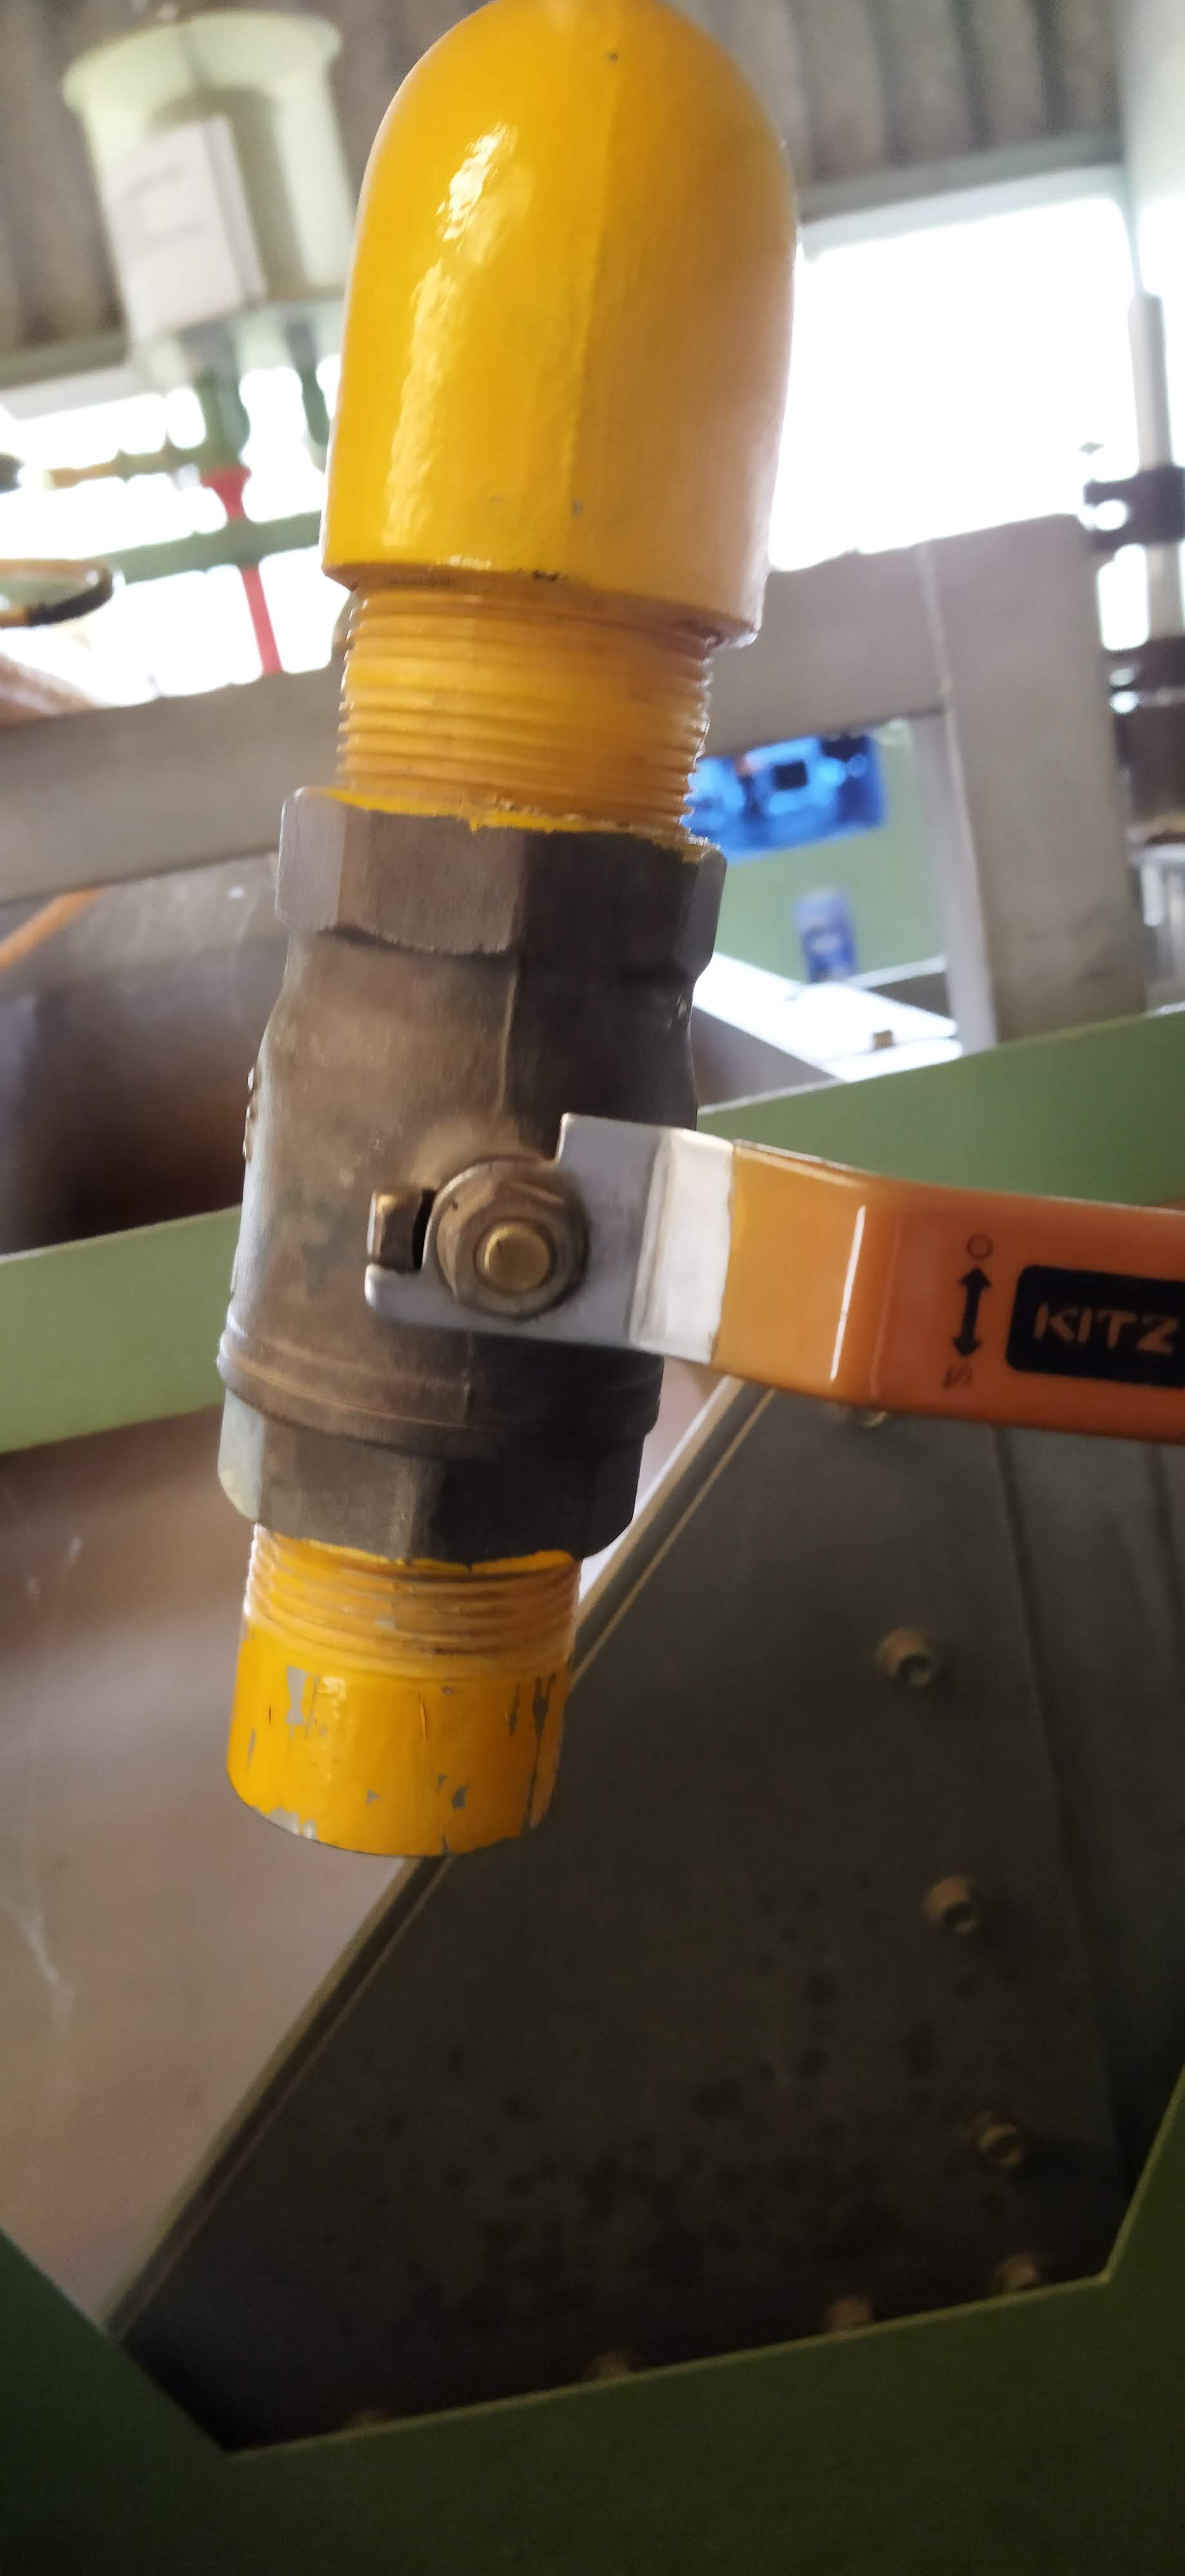
\includegraphics[height=0.25\textheight,keepaspectratio]{Figures/ballValve.jpg}
    \caption{Current discharge control unit}
    \label{fig:current_discharge_control_unit}
\end{figure}
\par
The $1 \frac{3}{4} inch $ ball valve on the main discharge pipe is opened in steps by hand using the lever. The size of a step is determined by intuition.
\par
\textbf{Design}\\
To ensure minimum modification of the existing machine, the automation of this unit utilized the existing ball valve. The opening and closing of the valve is automated using a motorized system that can open the valve in precise steps.
\par
\textbf{Motor}
\par
The selection and the sizing of the motor for this application was based on the following considerations:

\begin{enumerate}
    \item The torque required to open and close the ball valve.
    \item The steps size or the number of steps the system can open the valve.
\end{enumerate}
\par
Based on these two considerations, the following two applications were feasible.
\begin{enumerate}
    \item \textbf{Stepper Motor}\\
    This motor operates by accurately synchronizing position with the pulse signal output from the controller to the driver thus achieving highly accurate positioning and speed control. Stepper motors feature high torque and low vibration at low speeds ideally below 1500rpm, ideal for applications requiring quick fixed positioning in a short distance \cite{wargula2017investigations}. Furthermore, stepper motor rotates with a fixed step angle typically 1.8 degrees for a 2-phase. However, to achieve this requires the use of a micro-step driver.
    \par
    Besides having full control of rotation and speed, the simple structure of stepper motors is achieved without using electrical components, such as an encoder within the motor. For this reason, stepper motors are very robust and have high reliability with very few failures. As for stopping accuracy, ±0.05° (without cumulative pitch errors) is very accurate\cite{wargula2017investigations}. Because the positioning of stepper motors is performed by open-loop control, and operated by the magnetized stator and magnetic rotor with small teeth, stepper motors have a higher follow-up mechanism toward commands than the servo motors. Also, no hunting occurs when stopping it.
    
    \textbf{Design with stepper motor}
    \begin{enumerate}
    \item \textbf{Motor selection}\\
    From the stepper motors available in the market, Nema 17 Stepper motor shown in figure \ref{fig:Nema17 Steppper motor} was the best choice for the job since it can produce a $1.8^0$ step out of the box without a microstep driver. With the help of a microstep driver, it can produce as small as $1^0$ step.
    \begin{figure}[H]
        \centering
        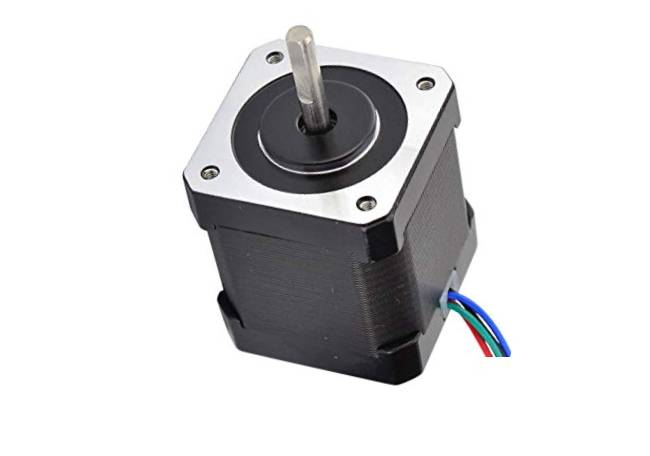
\includegraphics[width=.3\textwidth, height=.2\textheight]{Figures/Nema17Stepper.jpg}
        \caption[Nema 17 Stepper motor]{Nema 17 Stepper motor \cite{nema17}}
        \label{fig:Nema17 Steppper motor}
    \end{figure}
    \par
    Its technical specifications are as shown in the table below:
    \begin{table}[H]
\centering
\begin{tabular}{|l|l|}
\hline
\textbf{Property} & \textbf{Value} \\ \hline
Rated Voltage & 12V DC \\ \hline
Current & 1.2A at 4V \\ \hline
Step Angle & 1.8 deg \\ \hline
No. of Phases & 4 \\ \hline
Motor Length & 1.54 inches \\ \hline
4-wire, 8 inch lead &  \\ \hline
steps per revolution & 200 \\ \hline
Operating Temperature & -10 to 40 °C \\ \hline
Unipolar Holding Torque & 22.2 oz-in \\ \hline
Maximum torque & 4.8 Kg.cm \\ \hline
\end{tabular}
\caption[Nema 17 Stepper Motor Technical specification]{Nema 17 Stepper Motor Technical specification \cite{nema17}}
\end{table}
    \begin{figure}[H]
        \centering
        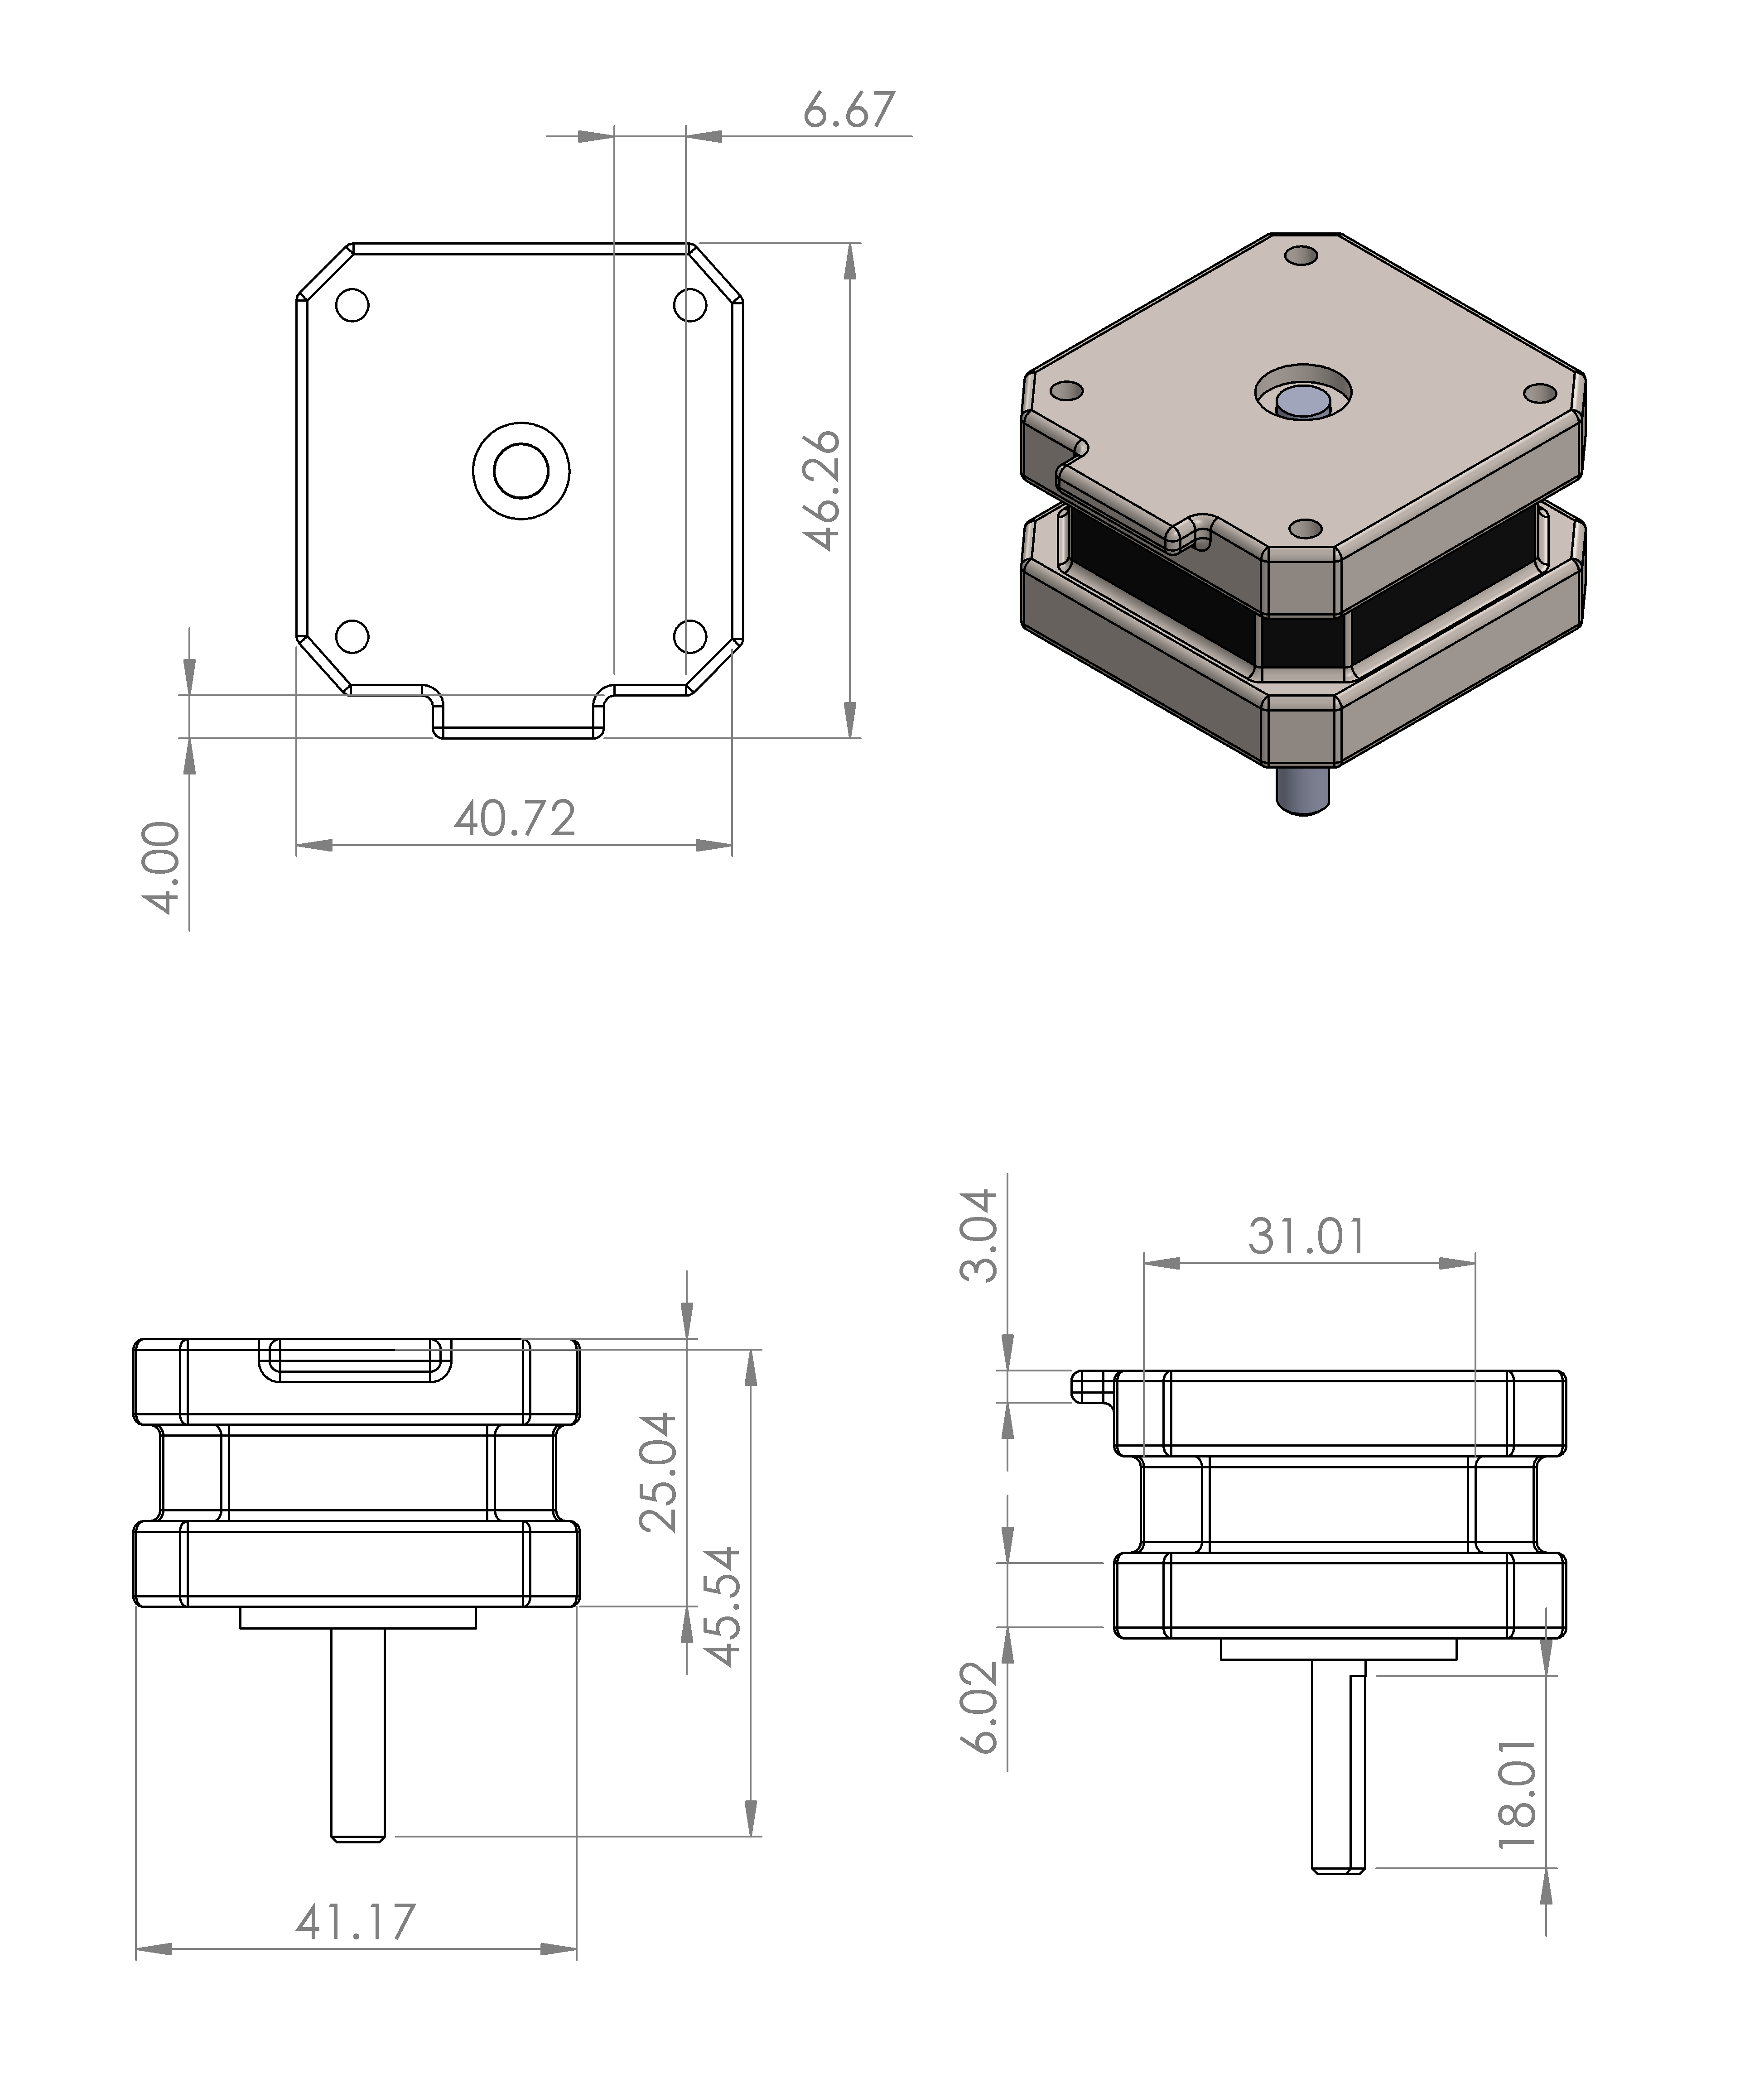
\includegraphics[height=.48\textheight]{Figures/Nema17StepperMotor.png}
        \caption{Nema 17 Stepper Motor Drawing}
        \label{fig:Nema17Drawing}
    \end{figure}
    Figure \ref{fig:Nema17Drawing} shows the actual dimensions of a nema 17 stepper motor. 
    \par
    \item \textbf{Ball valve - motor interface}
    \par
    An interface is required to connect the motor rotor to the ball valve. There were two option for this application:
    \begin{itemize}
        \item An interface that could fit the rotor on one end and with claw-like fingers on the other end to turn the existing ball valve's lever.
        \item An interface that could fit the rotor on one end and with the other end, similar to the lever, that could be used in place of the lever.
    \end{itemize}
    \par
    The second option was chosen since the first choice will introduce a lag in a turn action since the point of action on the lever is displaced from the line of rotation of the rotor.
    \begin{figure}[H]
        \centering
        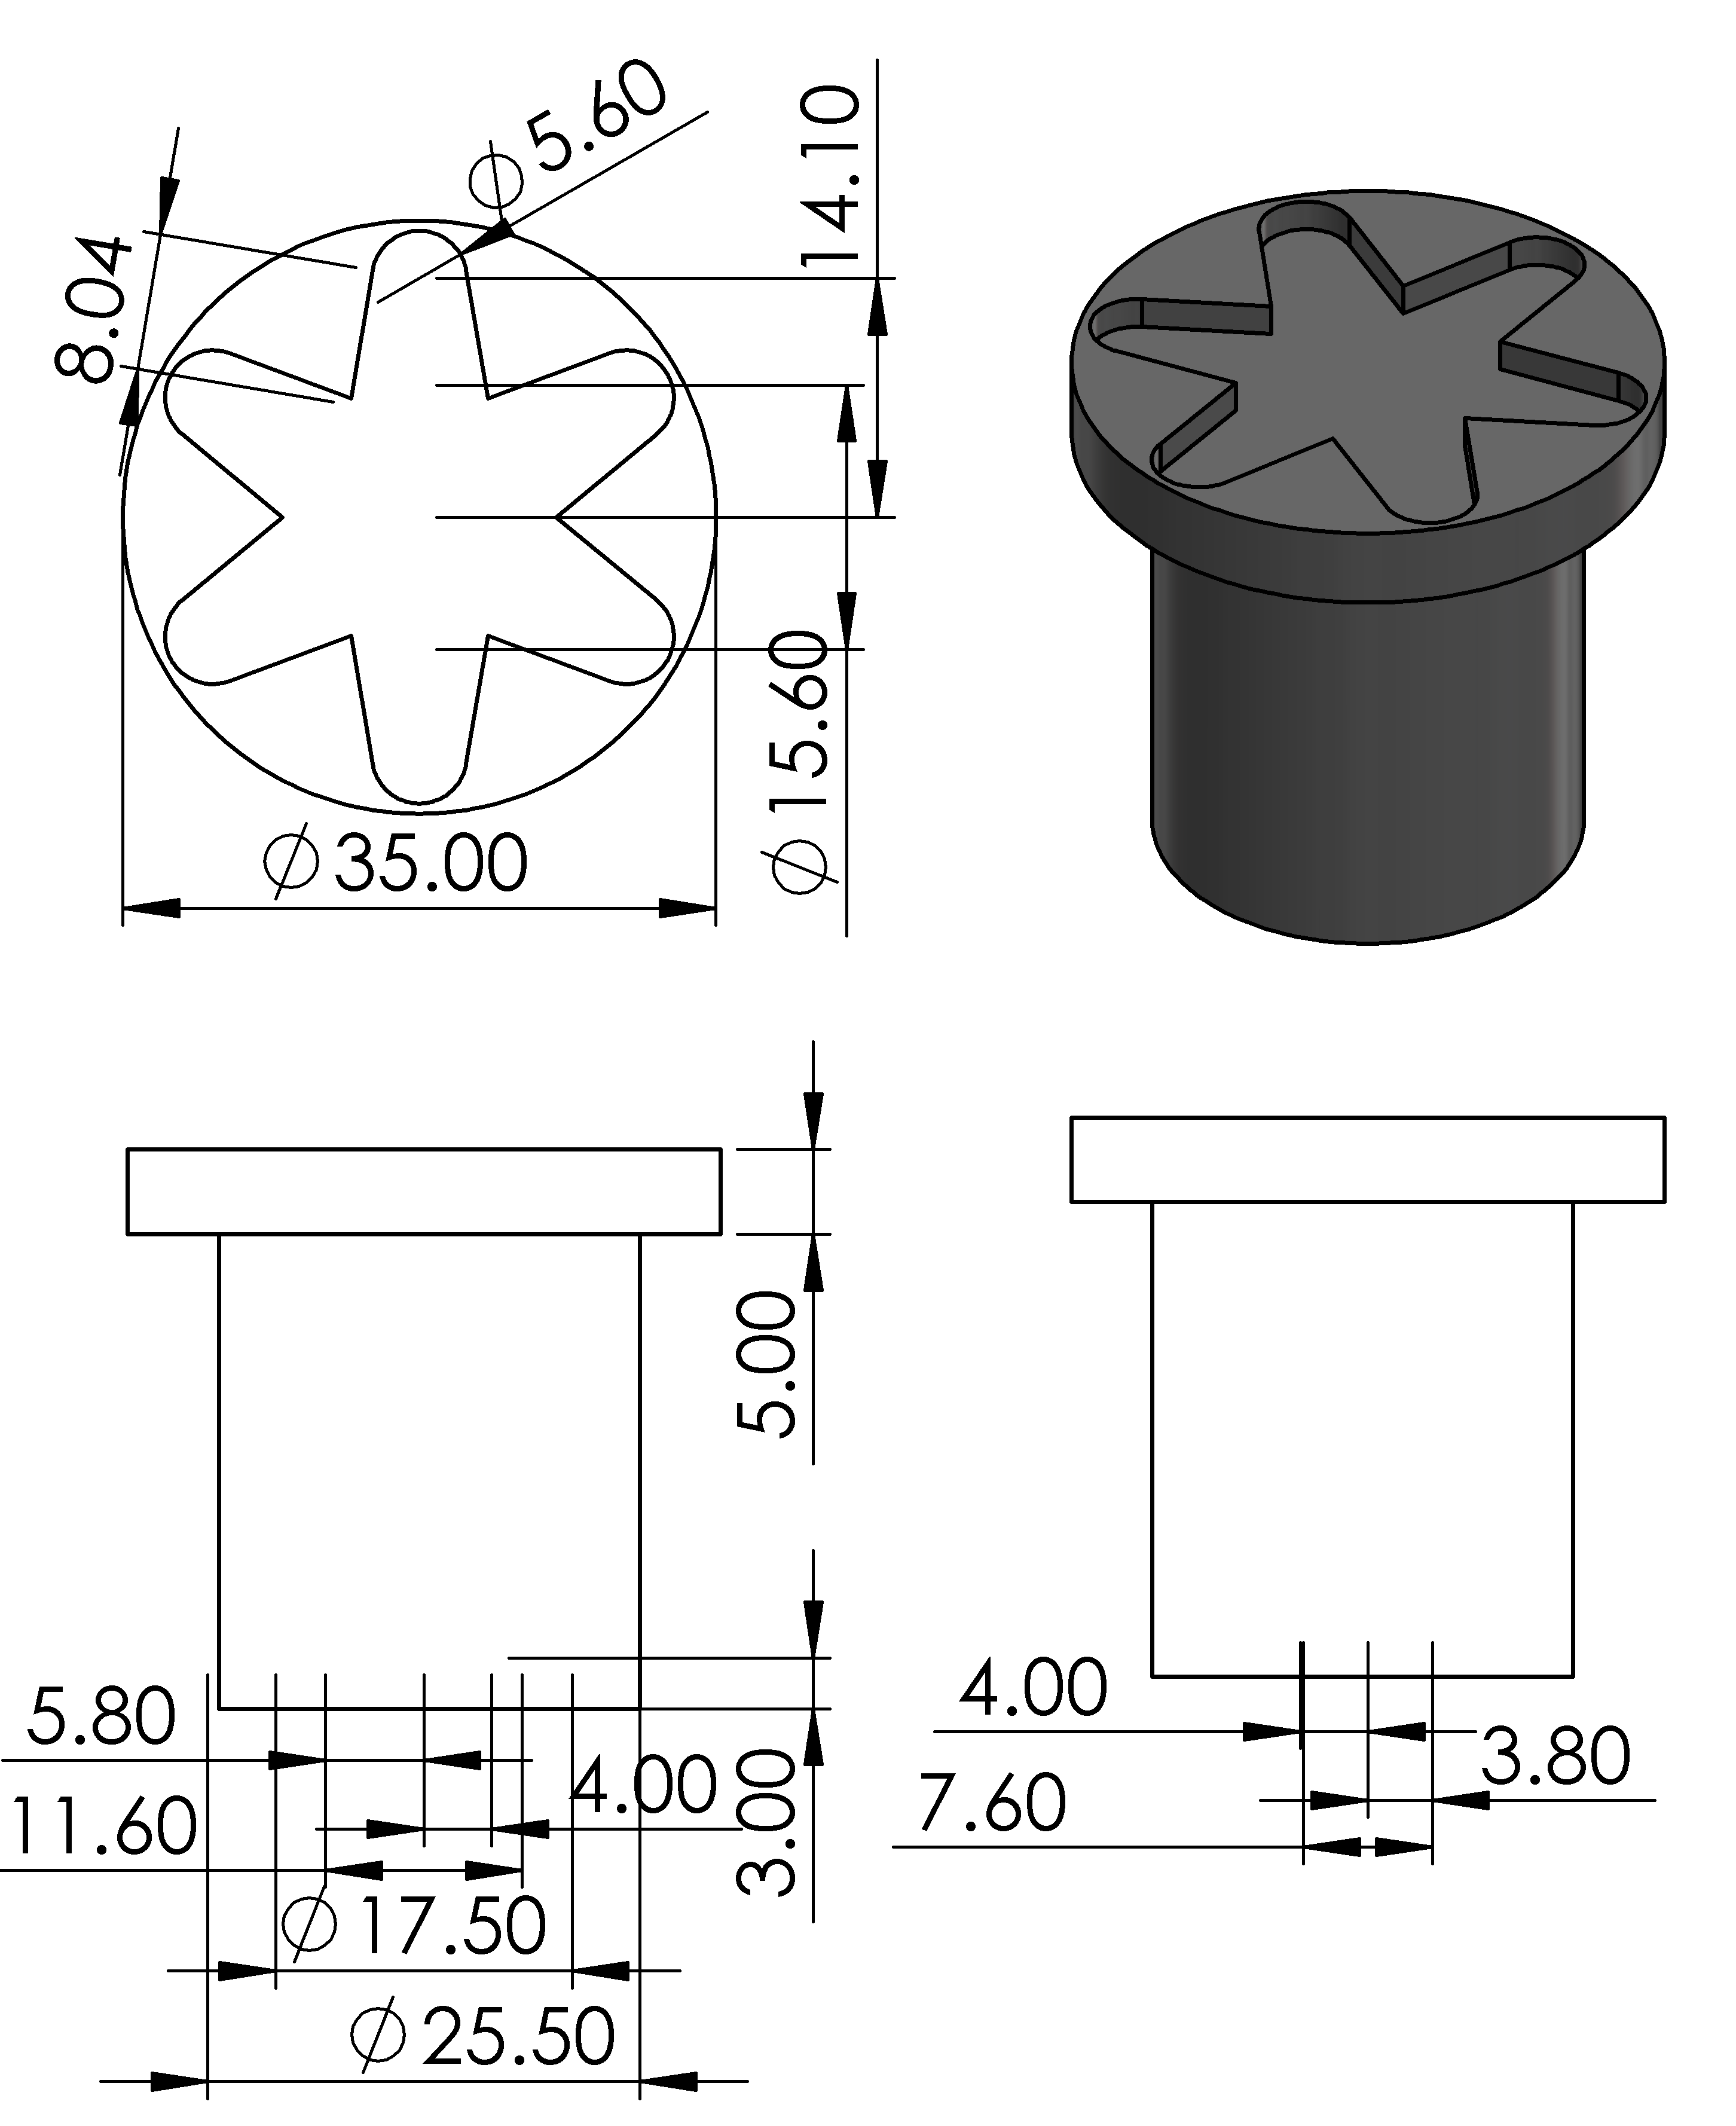
\includegraphics[height=0.5\textheight]{Figures/Interface.PNG}
        \caption{Interface}
        \label{fig:Interface}
    \end{figure}
    Figure \ref{fig:Interface} shows the interface design. Dimensions of the interface, such as the width of its base, were measured and transferred from the existing lever.
    \par
    \item \textbf{Motor cage}
    \par
    In order to support the motor on the ball valve, a motor cage was designed to fit the motor as shown in Figure \ref{fig:motor_cage_stepper}.
    
    \begin{figure}[H]
        \centering
        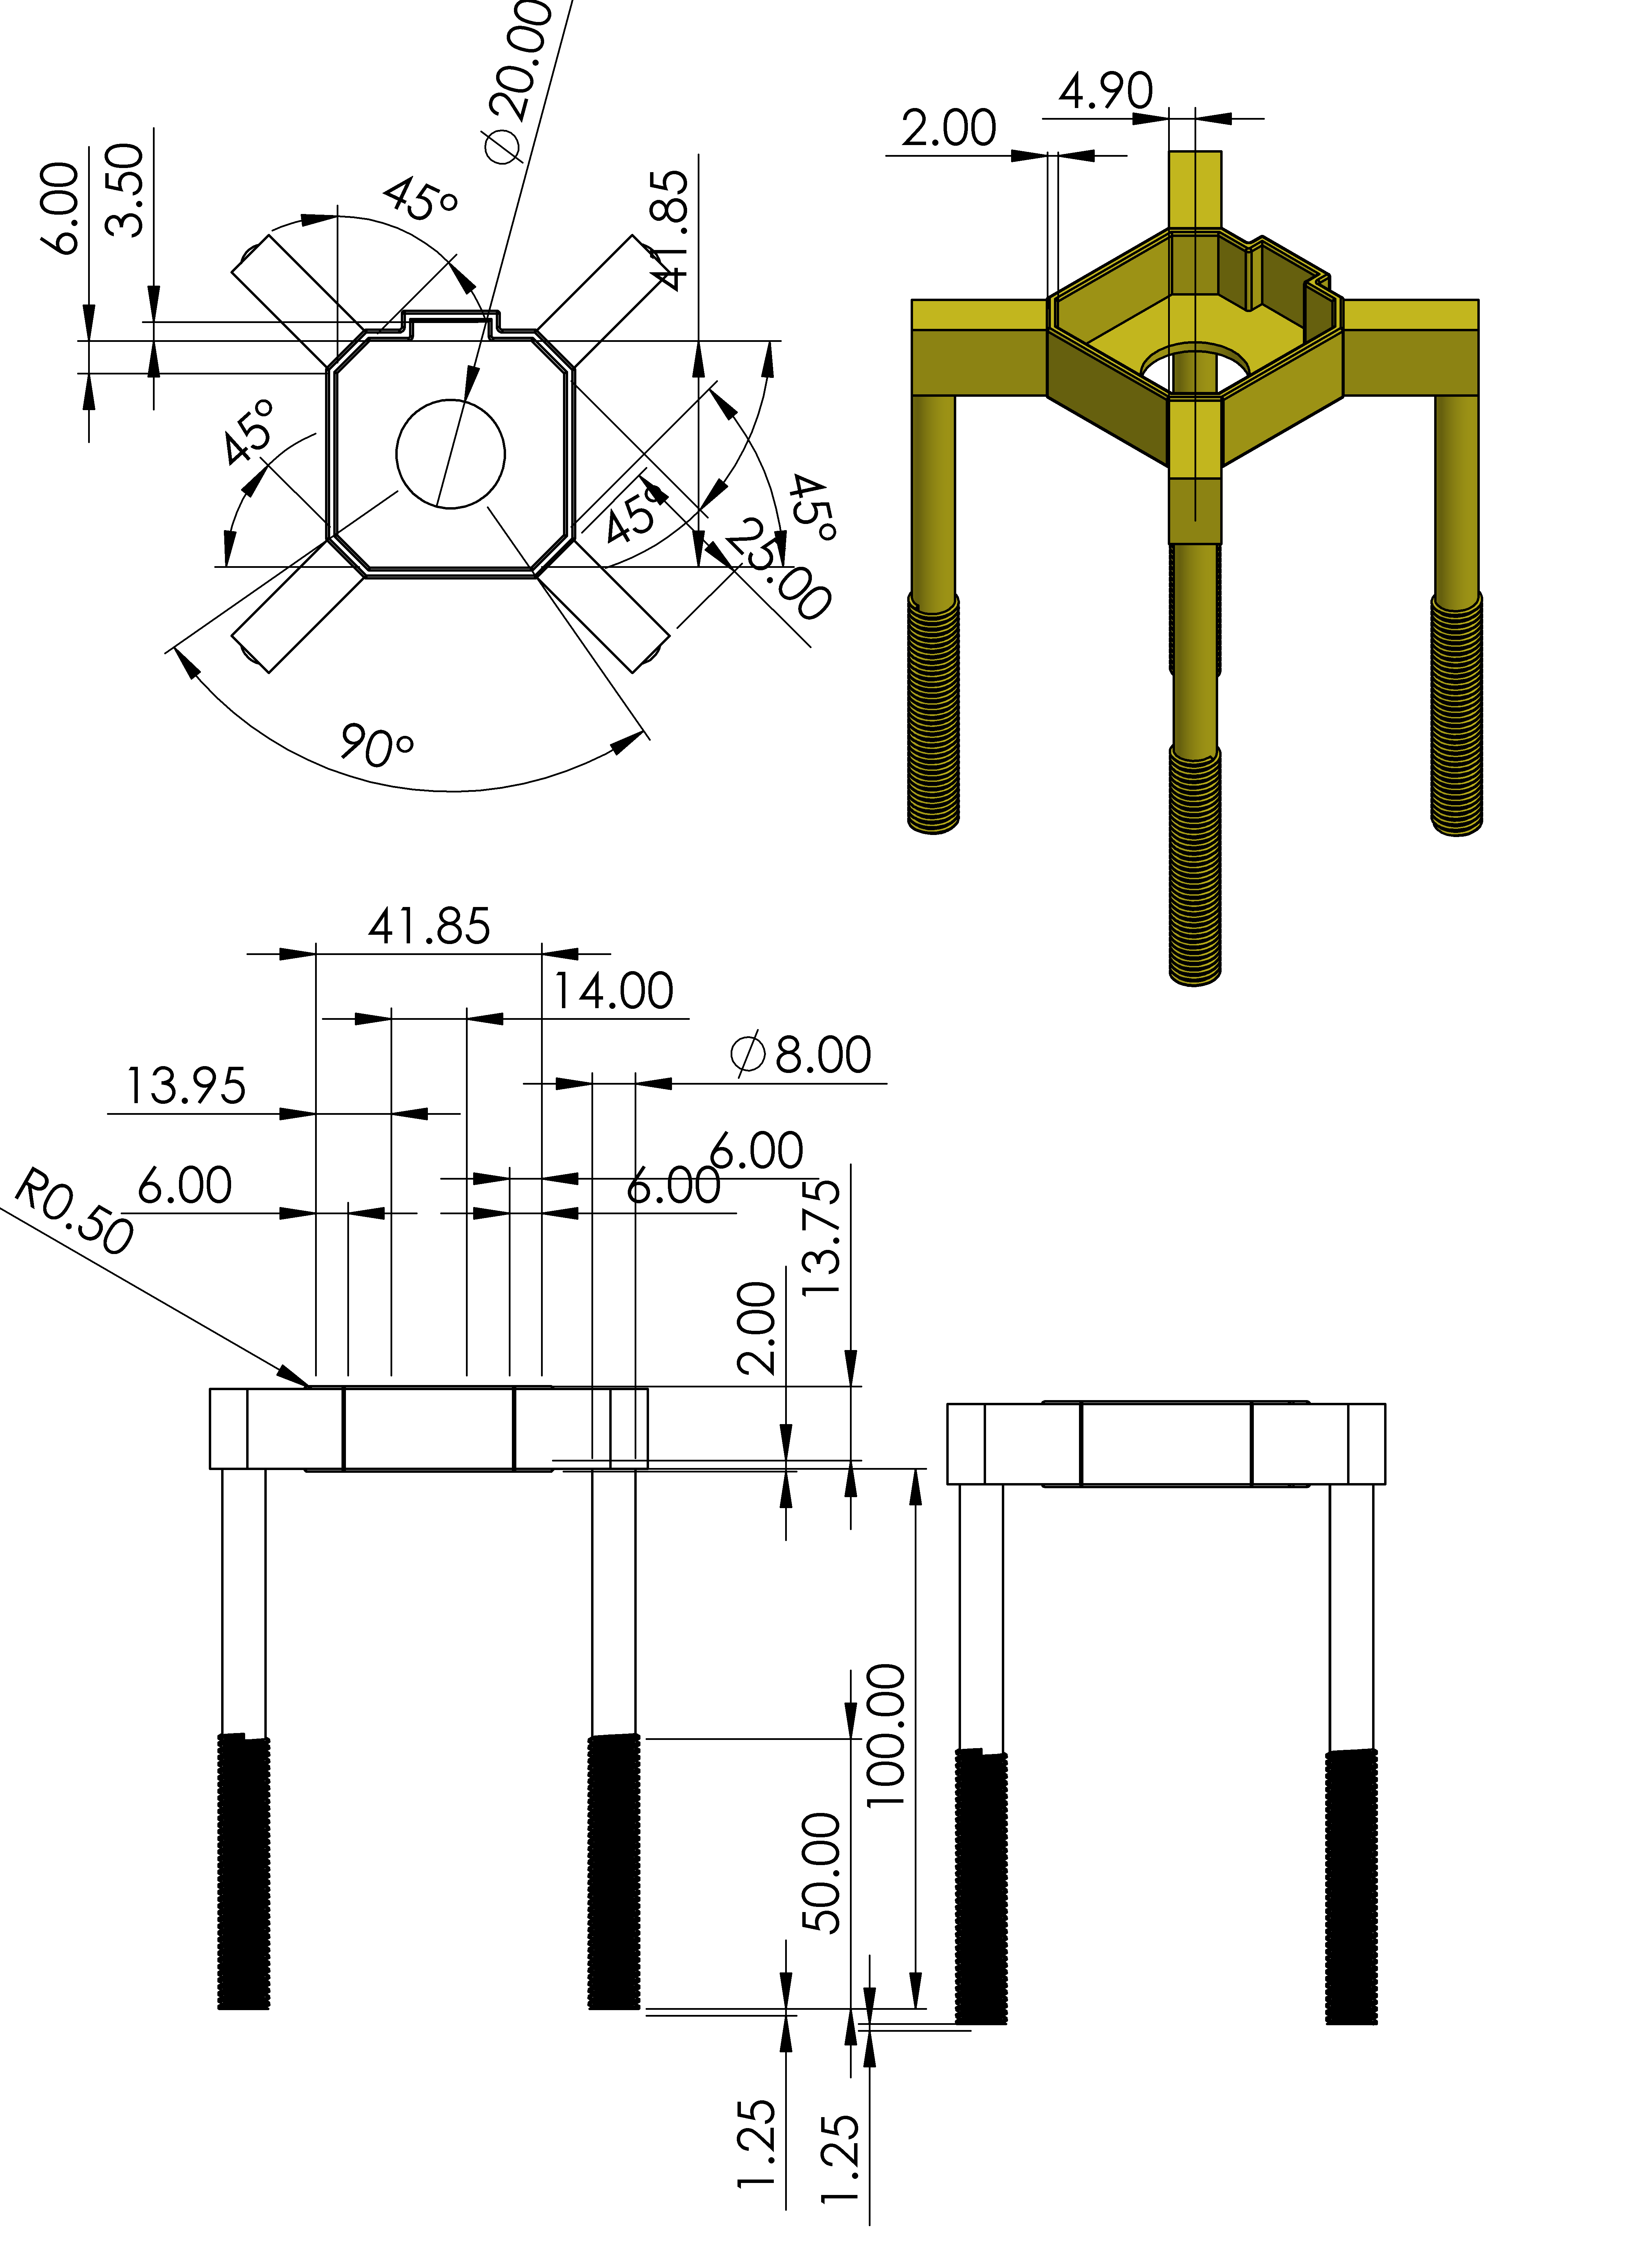
\includegraphics[height=.75\textheight]{Figures/MotorCage.PNG}
        \caption{Motor Cage}
        \label{fig:motor_cage_stepper}
    \end{figure}
    
    The dimensions of the motor cage in figure \ref{fig:motor_cage_stepper} were determined from that of the stepper motor, the motor-ball valve interface, and that of the existing ball valve socket shown in figure \ref{fig:ball_valve_socket}.
    
    \begin{figure}[H]
        \centering
        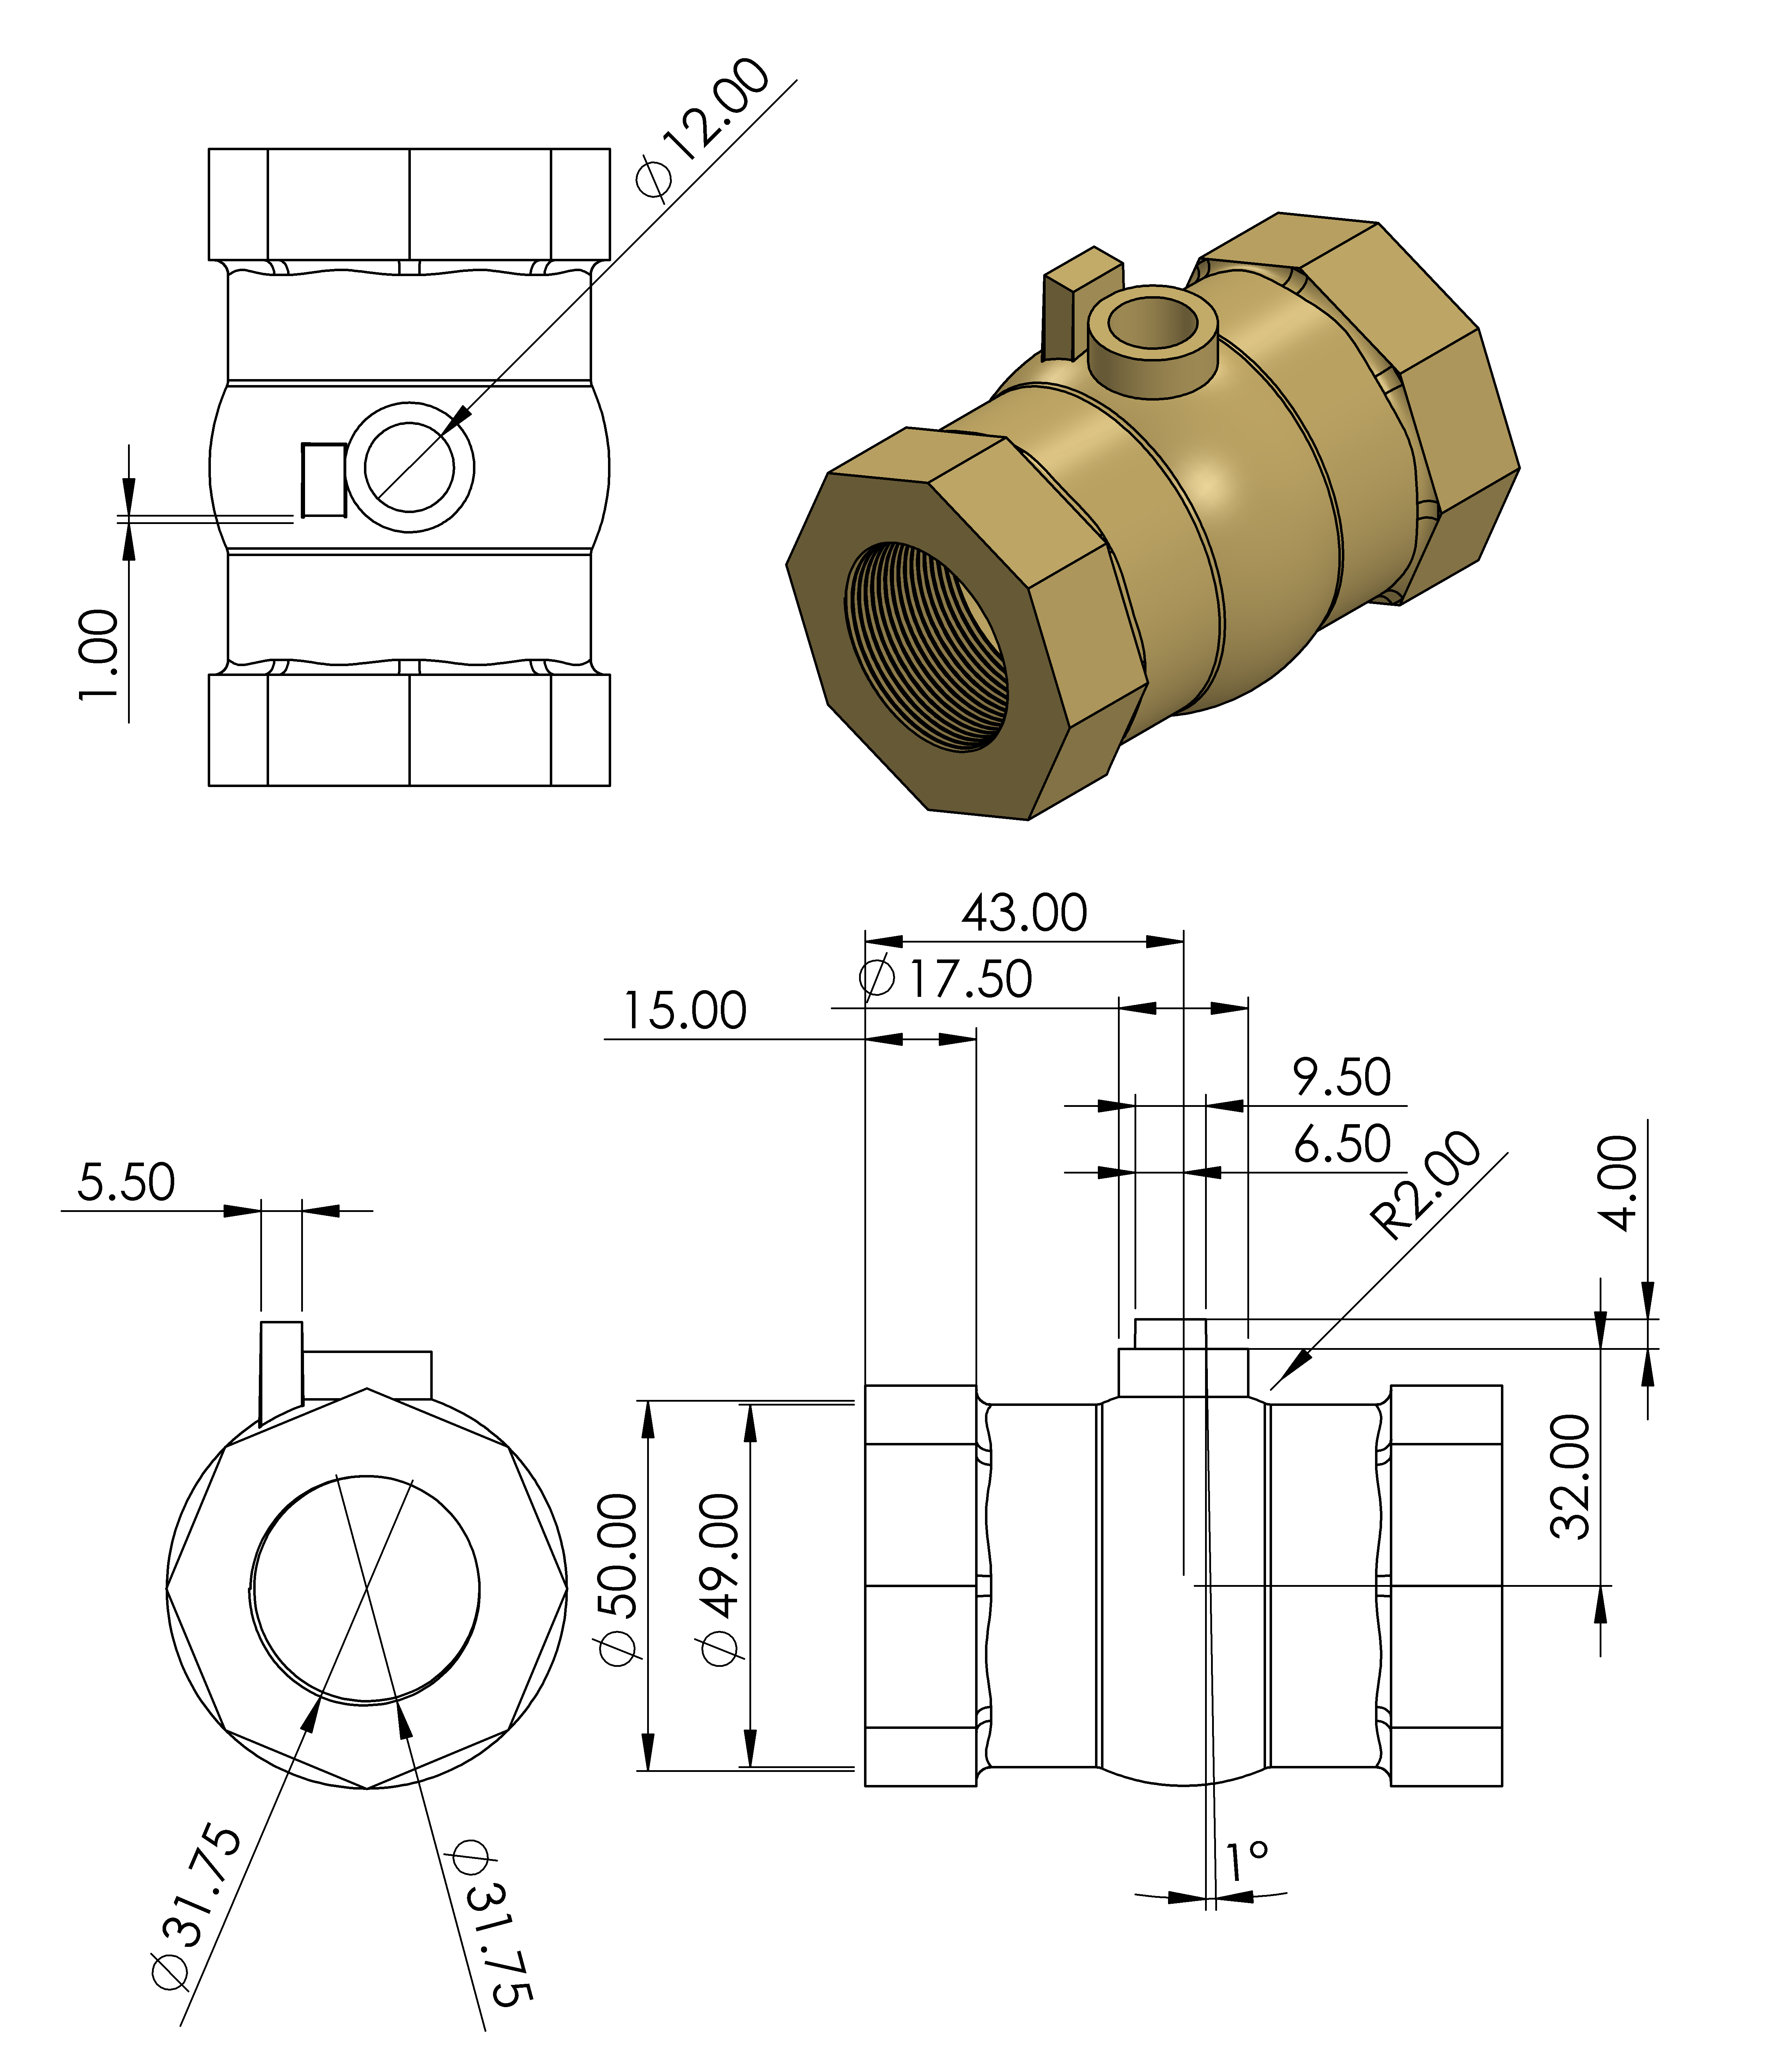
\includegraphics[height=.8\textheight]{Figures/socket.PNG}
        \caption{Ball valve socket}
        \label{fig:ball_valve_socket}
    \end{figure}
    \item \textbf{Straps}
    \par
    The motor cage with the stepper motor mounted is mounted on the main discharge pipe using straps, one of which is shown in figure \ref{fig:mounting_straps_stepper}.
    
    \begin{figure}[H]
        \centering
        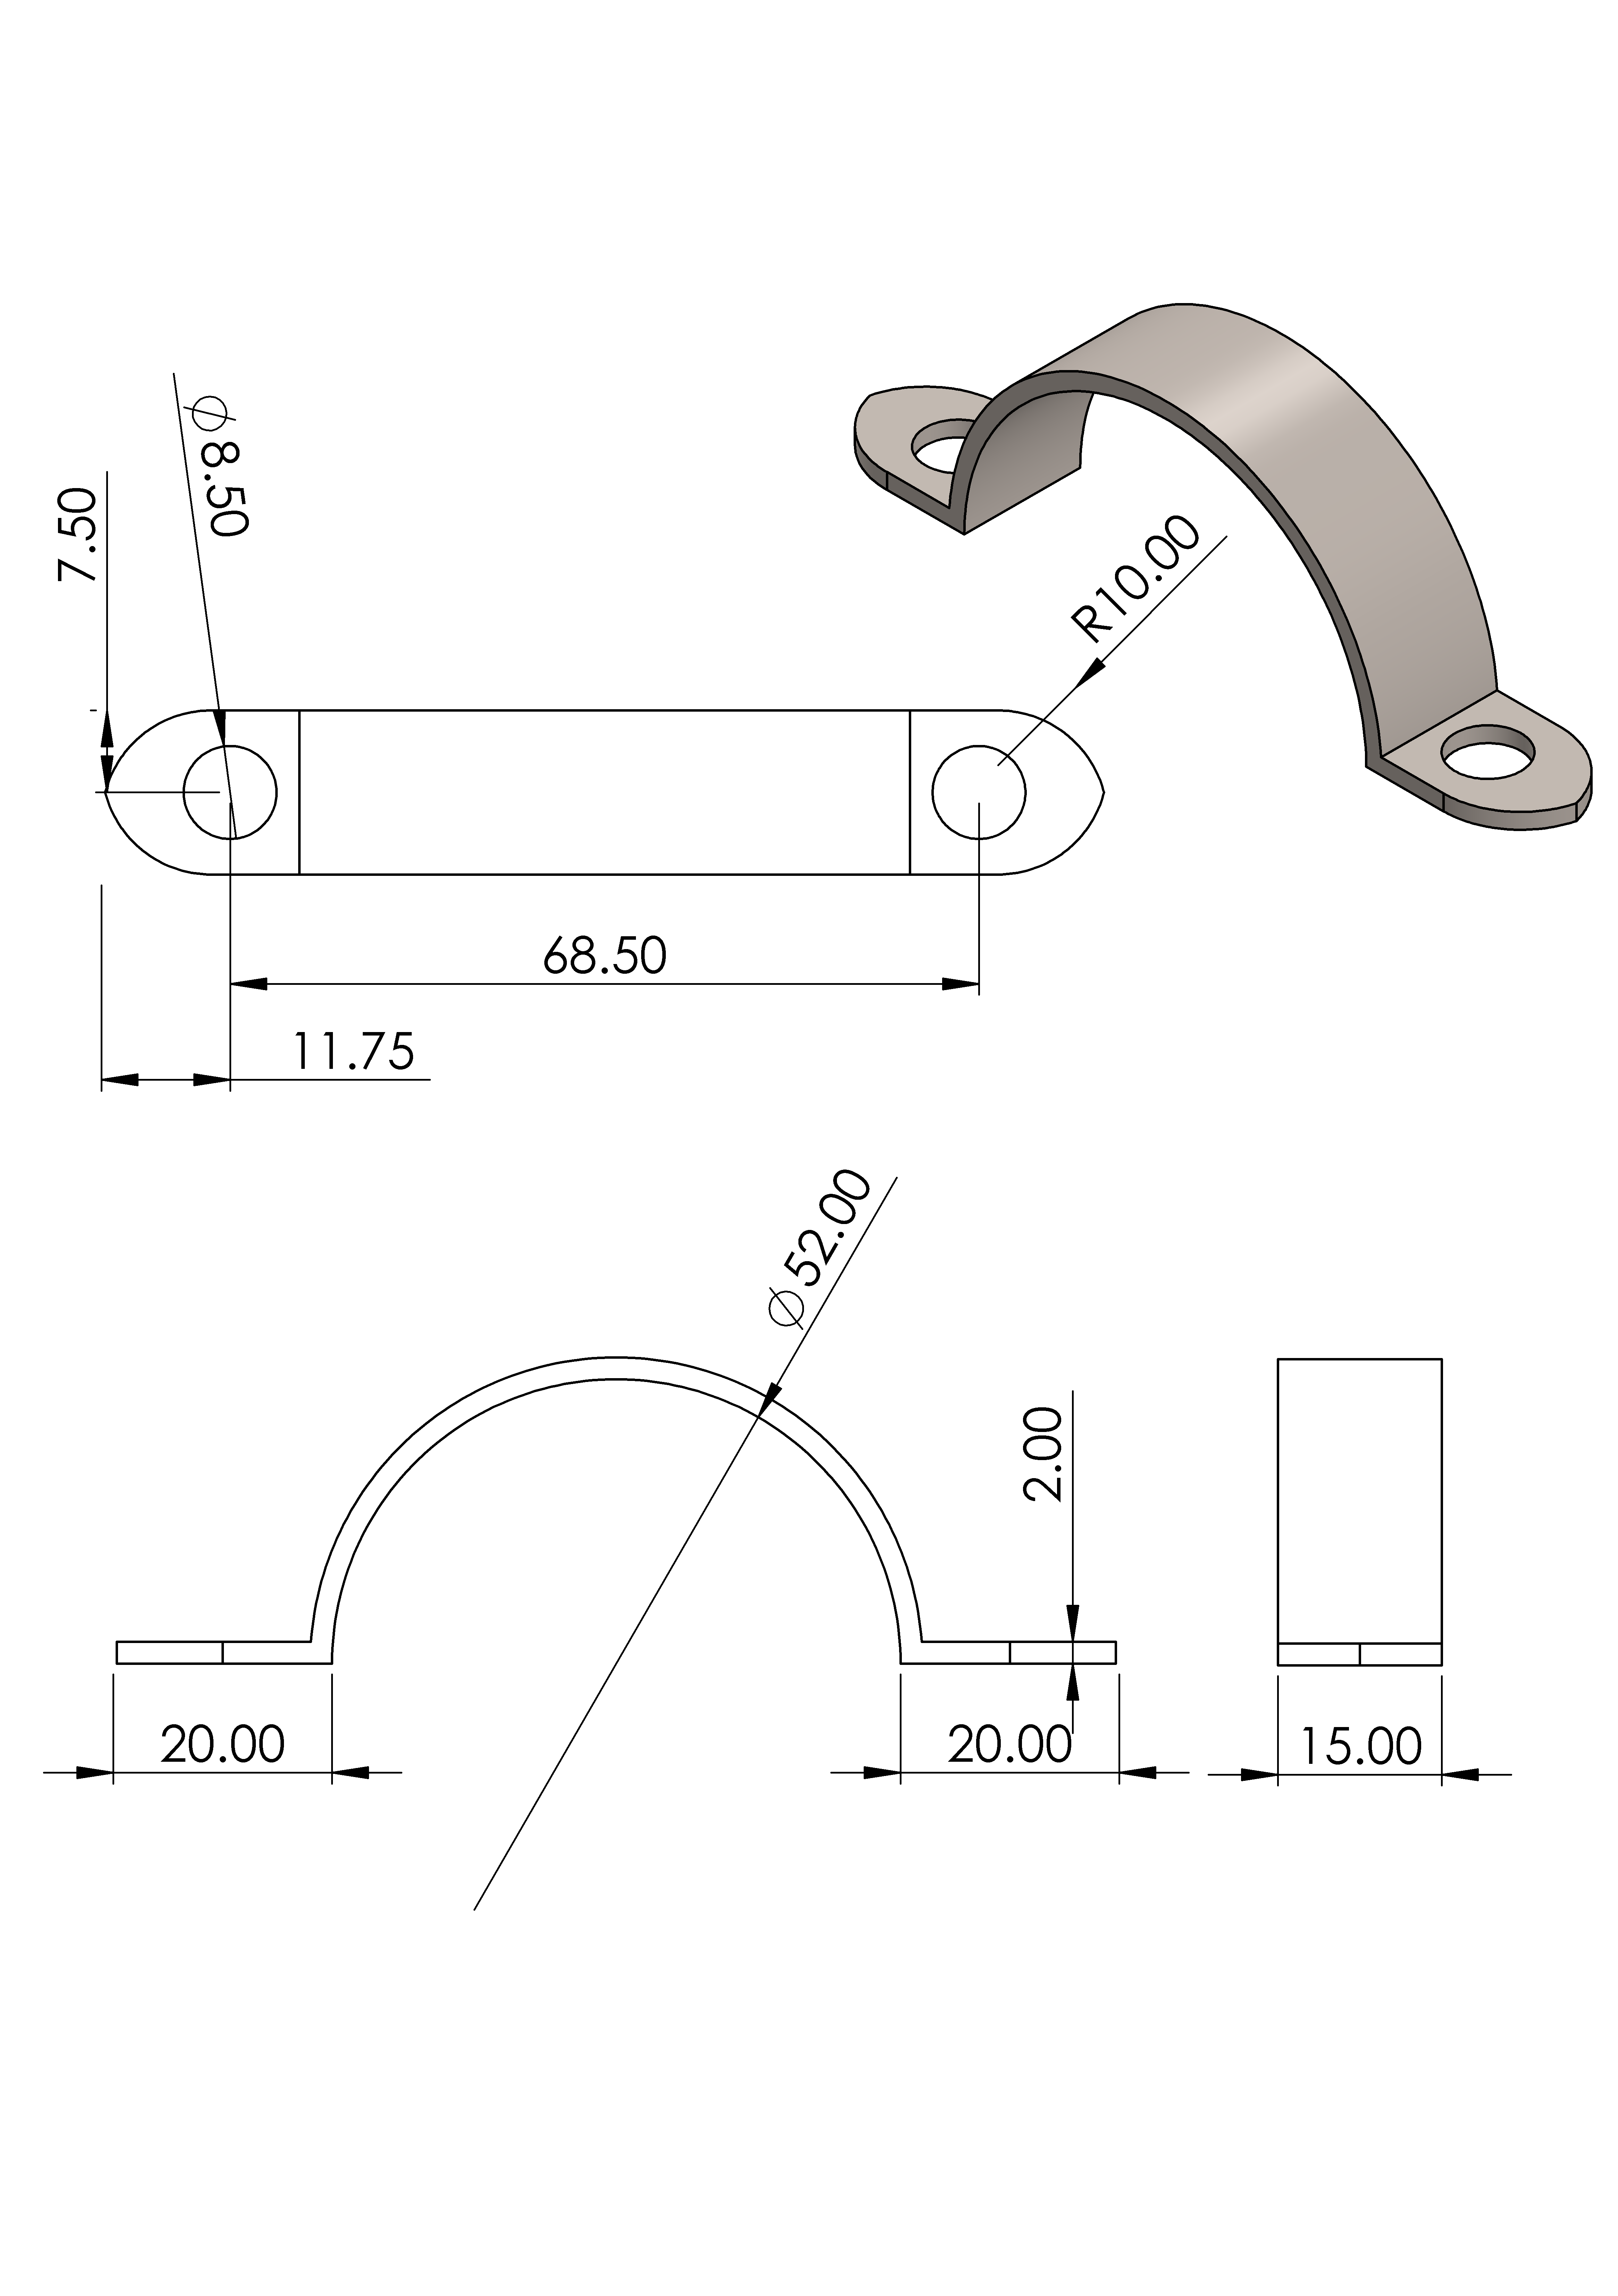
\includegraphics[height=.6\textheight]{Figures/strap.PNG}
        \caption{Mounting straps}
        \label{fig:mounting_straps_stepper}
    \end{figure}
    
    \item \textbf{Assembly of discharge flow control using stepper}
    \par
    The assembly of the discharge control unit is as shown in figure \ref{fig:stepper_actuated_ball_valve}. Nuts are used to fasten the whole structure on the main discharge pipe.
    
    \begin{figure}[H]
        \centering
        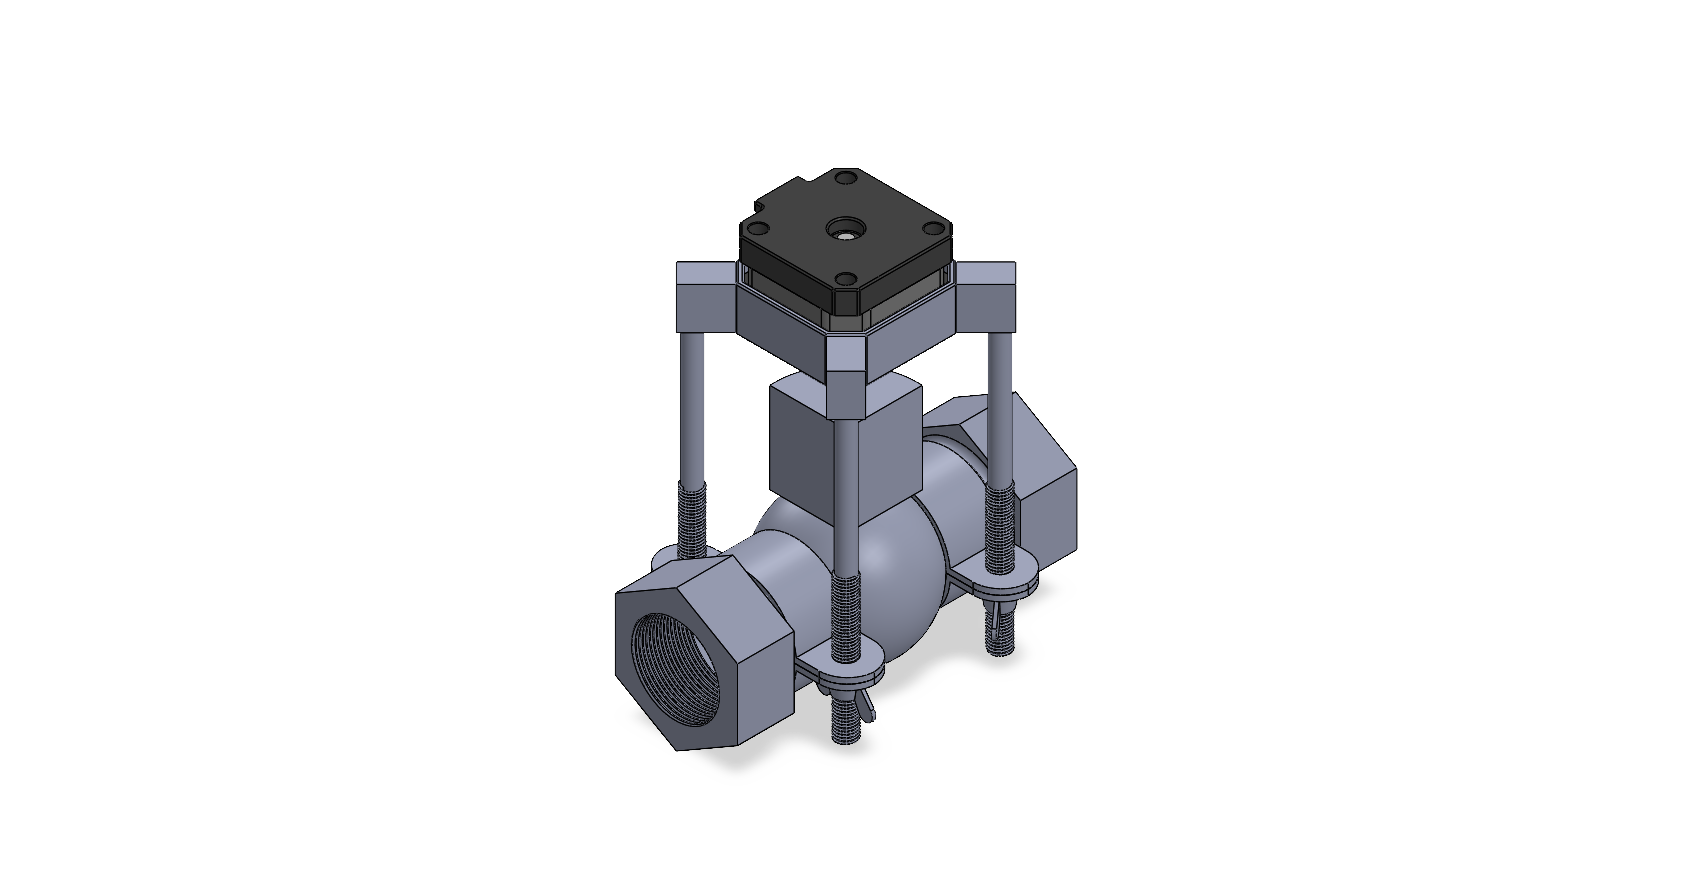
\includegraphics{Figures/ActuatedBallValve.PNG}
        \caption{Stepper Actuated ball valve}
        \label{fig:stepper_actuated_ball_valve}
    \end{figure}
    
    \item \textbf{Finite element analysis of the assembly}
    \par
    The assembly was stress tested by applying a torque on the motor cage to determine if it could hold at the maximum torque of the motor. To do this, each part of this assembly was be assigned a material. Polyactic acid (PLA) was selected as the common material for all of the parts in the assembly. This is majorly due to the following reasons:
    \begin{itemize}
        \item The maximum weight of the part to be supported by the structure is the stepper motor's weight, 450 grams. This can be supported by a 3D printed plastic support. A lighter material such as fiber glass or carbon fiber could be used but they are costlier than the set project's budget.
        \item The parts are complex for fabrication on the currently existing machinery in the university.
    \end{itemize}
    \par
    \item \textbf{Results}
    \par
    As shown in figure \ref{fig:SimulationResults}, the structure holds for the maximum torque of a Nema 17 stepper motor, $4.9 kg.cm$ or $0.4707192 Nm$.
    \begin{figure}[H]
        \centering
        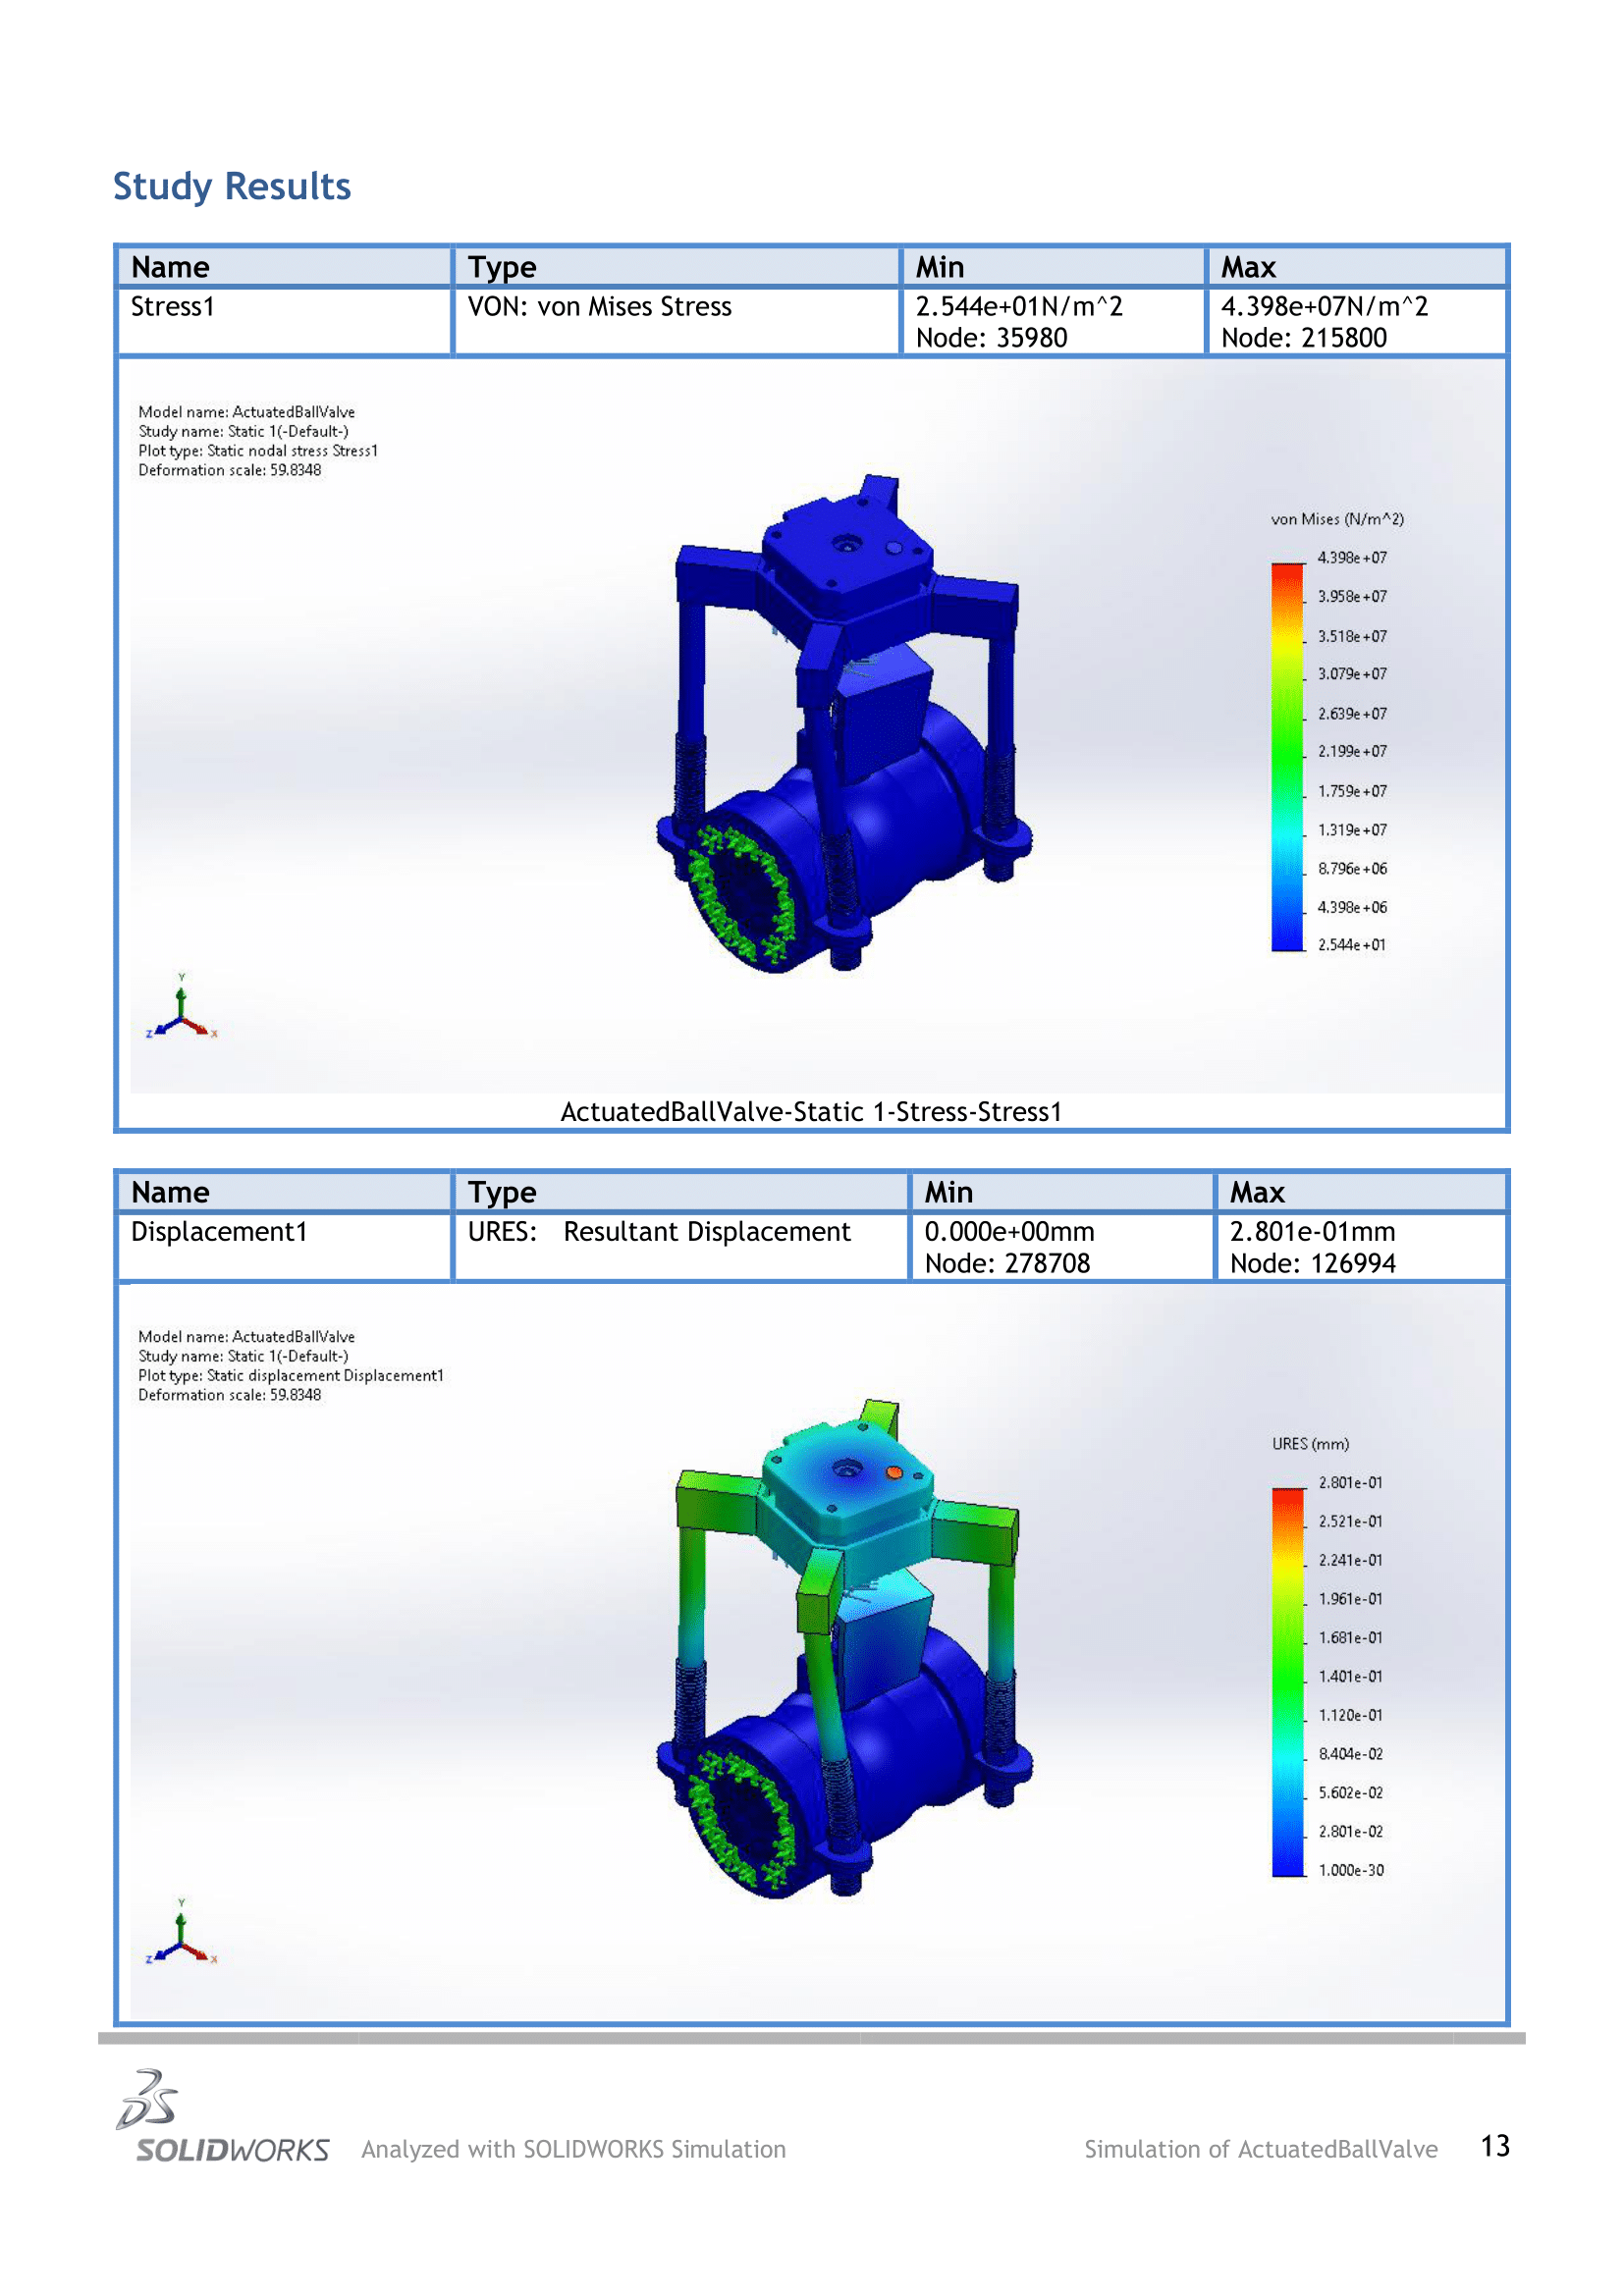
\includegraphics[width=\textwidth]{Figures/ActuatedBallValve-Static-1-1-1.png}
        \caption{Simulation results}
        \label{fig:SimulationResults}
    \end{figure}
    
     
    \end{enumerate}
    
    
    \item \textbf{Servo Motor}\\
    Servo motors run significantly faster than stepper motors, with speeds greater than 1500 rpm \cite{halicioglu2016mechanisms}. This enables servomotors to be used with gearboxes to deliver much higher torque at useful speeds. They also deliver more consistent torque across the speed range of the motor. Unlike stepper motors, they do not have holding torque. Closed-loop operation enables the controller/drive to command that the load remain at a specific position, however, and the motor will make continual adjustments to hold it there. Thus, servomotors can produce de facto holding torque\cite{halicioglu2016mechanisms}. The Servo motor rotates with a fixed step angle as low as 1 degree with or without the use of a driver. Furthermore, when powered, servomotors tend to move their shaft position to zero, a phenomenon known as hunting.
    \par
    \textbf{Design with servo motor}
    \begin{enumerate}
    \par
    \item \textbf{Motor selection}
    \par
    An MG996R Servo motor shown in figure \ref{fig:servo_motor_assembly} was the best choice among many servo motors found in the market. It is the motor that provided the torque required to turn the ball valve at an optimum price for the project's budget. 
    \par
    The motor specification as shown in table \ref{tab:MG996R_servo_specs}.
    \begin{table}[H]
    \centering
    \begin{tabular}{|l|l|}
    \hline
    \textbf{Property} & \textbf{Value} \\ \hline
    Operating Voltage & +5V \\ \hline
    Current & 2.5A (6V) \\ \hline
    Stall Torque & 9.4 kg/cm (at 4.8V) \\ \hline
    Maximum Stall Torque & 11 kg/cm (6V) \\ \hline
    Operating speed & 0.17 s/60° \\ \hline
    Gear Type & Metal \\ \hline
    Rotation & 0°-180° \\ \hline
    Weight of motor & 55gm \\ \hline
    \end{tabular}
    \caption[MG996R Servo motor specifications]{MG996R Servo motor specifications \cite{mg996r}}
    \label{tab:MG996R_servo_specs}
    \end{table}
    \begin{figure}[H]
        \centering
        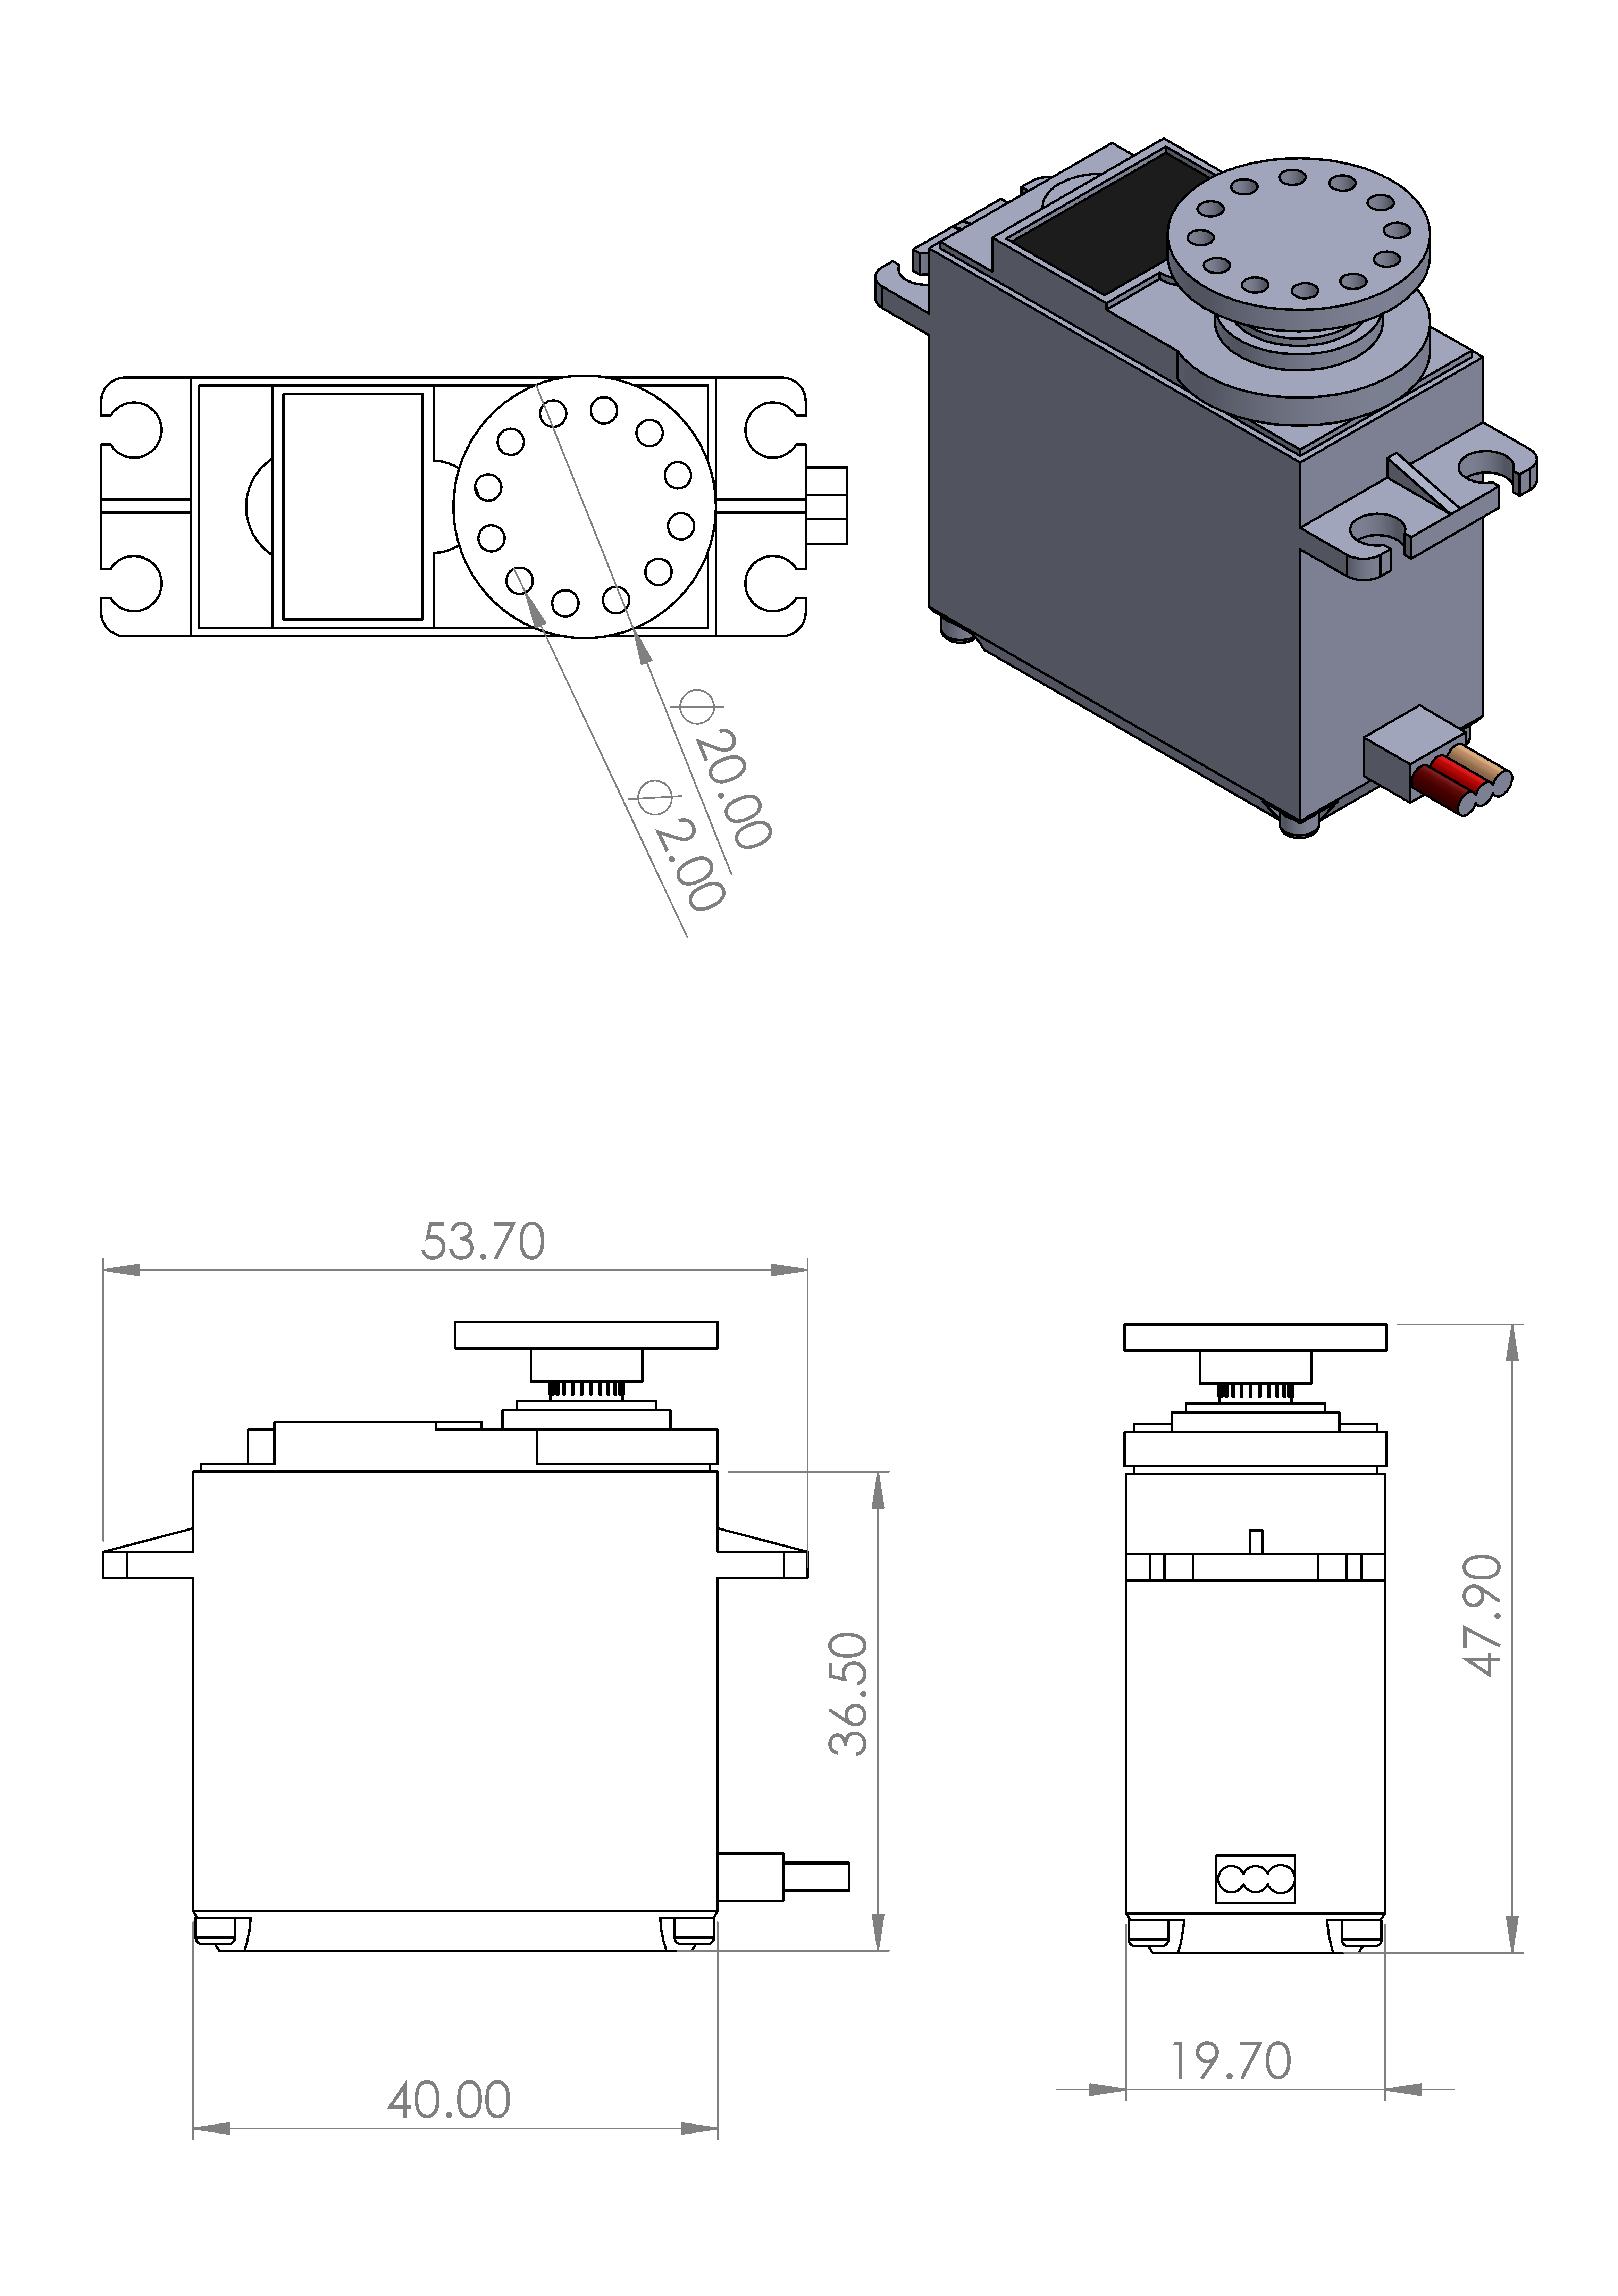
\includegraphics{Figures/ServoMotorAssembly.PNG}
        \caption{MG996R servo motor}
        \label{fig:servo_motor_assembly}
    \end{figure}
    The mounting mechanism of a servo motor is not as direct as that of the stepper motor since a servo motor homes to $0^{0}$ on powering. It is required that the home position of the servo motor is equal to the closed position of the ball valve. Therefore, during mounting, the servo motor must be rotated to align its home position with the closed position of the ball valve.
    \par
    The mounting mechanism should therefore allow for this rotation. A cuboid cage could have been used to support the motor in place, but since the centre of mass of this motor is displaced from its line of axle rotation, rotating the cuboid could mean repositioning the support stands for the cuboid.
    \par
     There were two options that could achieve this kind of rotation:
     \begin{enumerate}
         \item A combination of a cuboid cage on a circular plate. The cuboid cage could hold the motor while the plate allows the rotation of the assembly of the two without the need of repositioning the stands holding the assembly on the ball valve.
         \par
         \textbf{Designs with this approach}
         \par
         \begin{itemize}
             \item \textbf{Servo motor cage}
            \par
            The cage shown in figure \ref{fig:servo_motor_cage} is screwed on to the motor flaps. It just adds additional mounting points for the motor. 
            \begin{figure}[H]
                \centering
                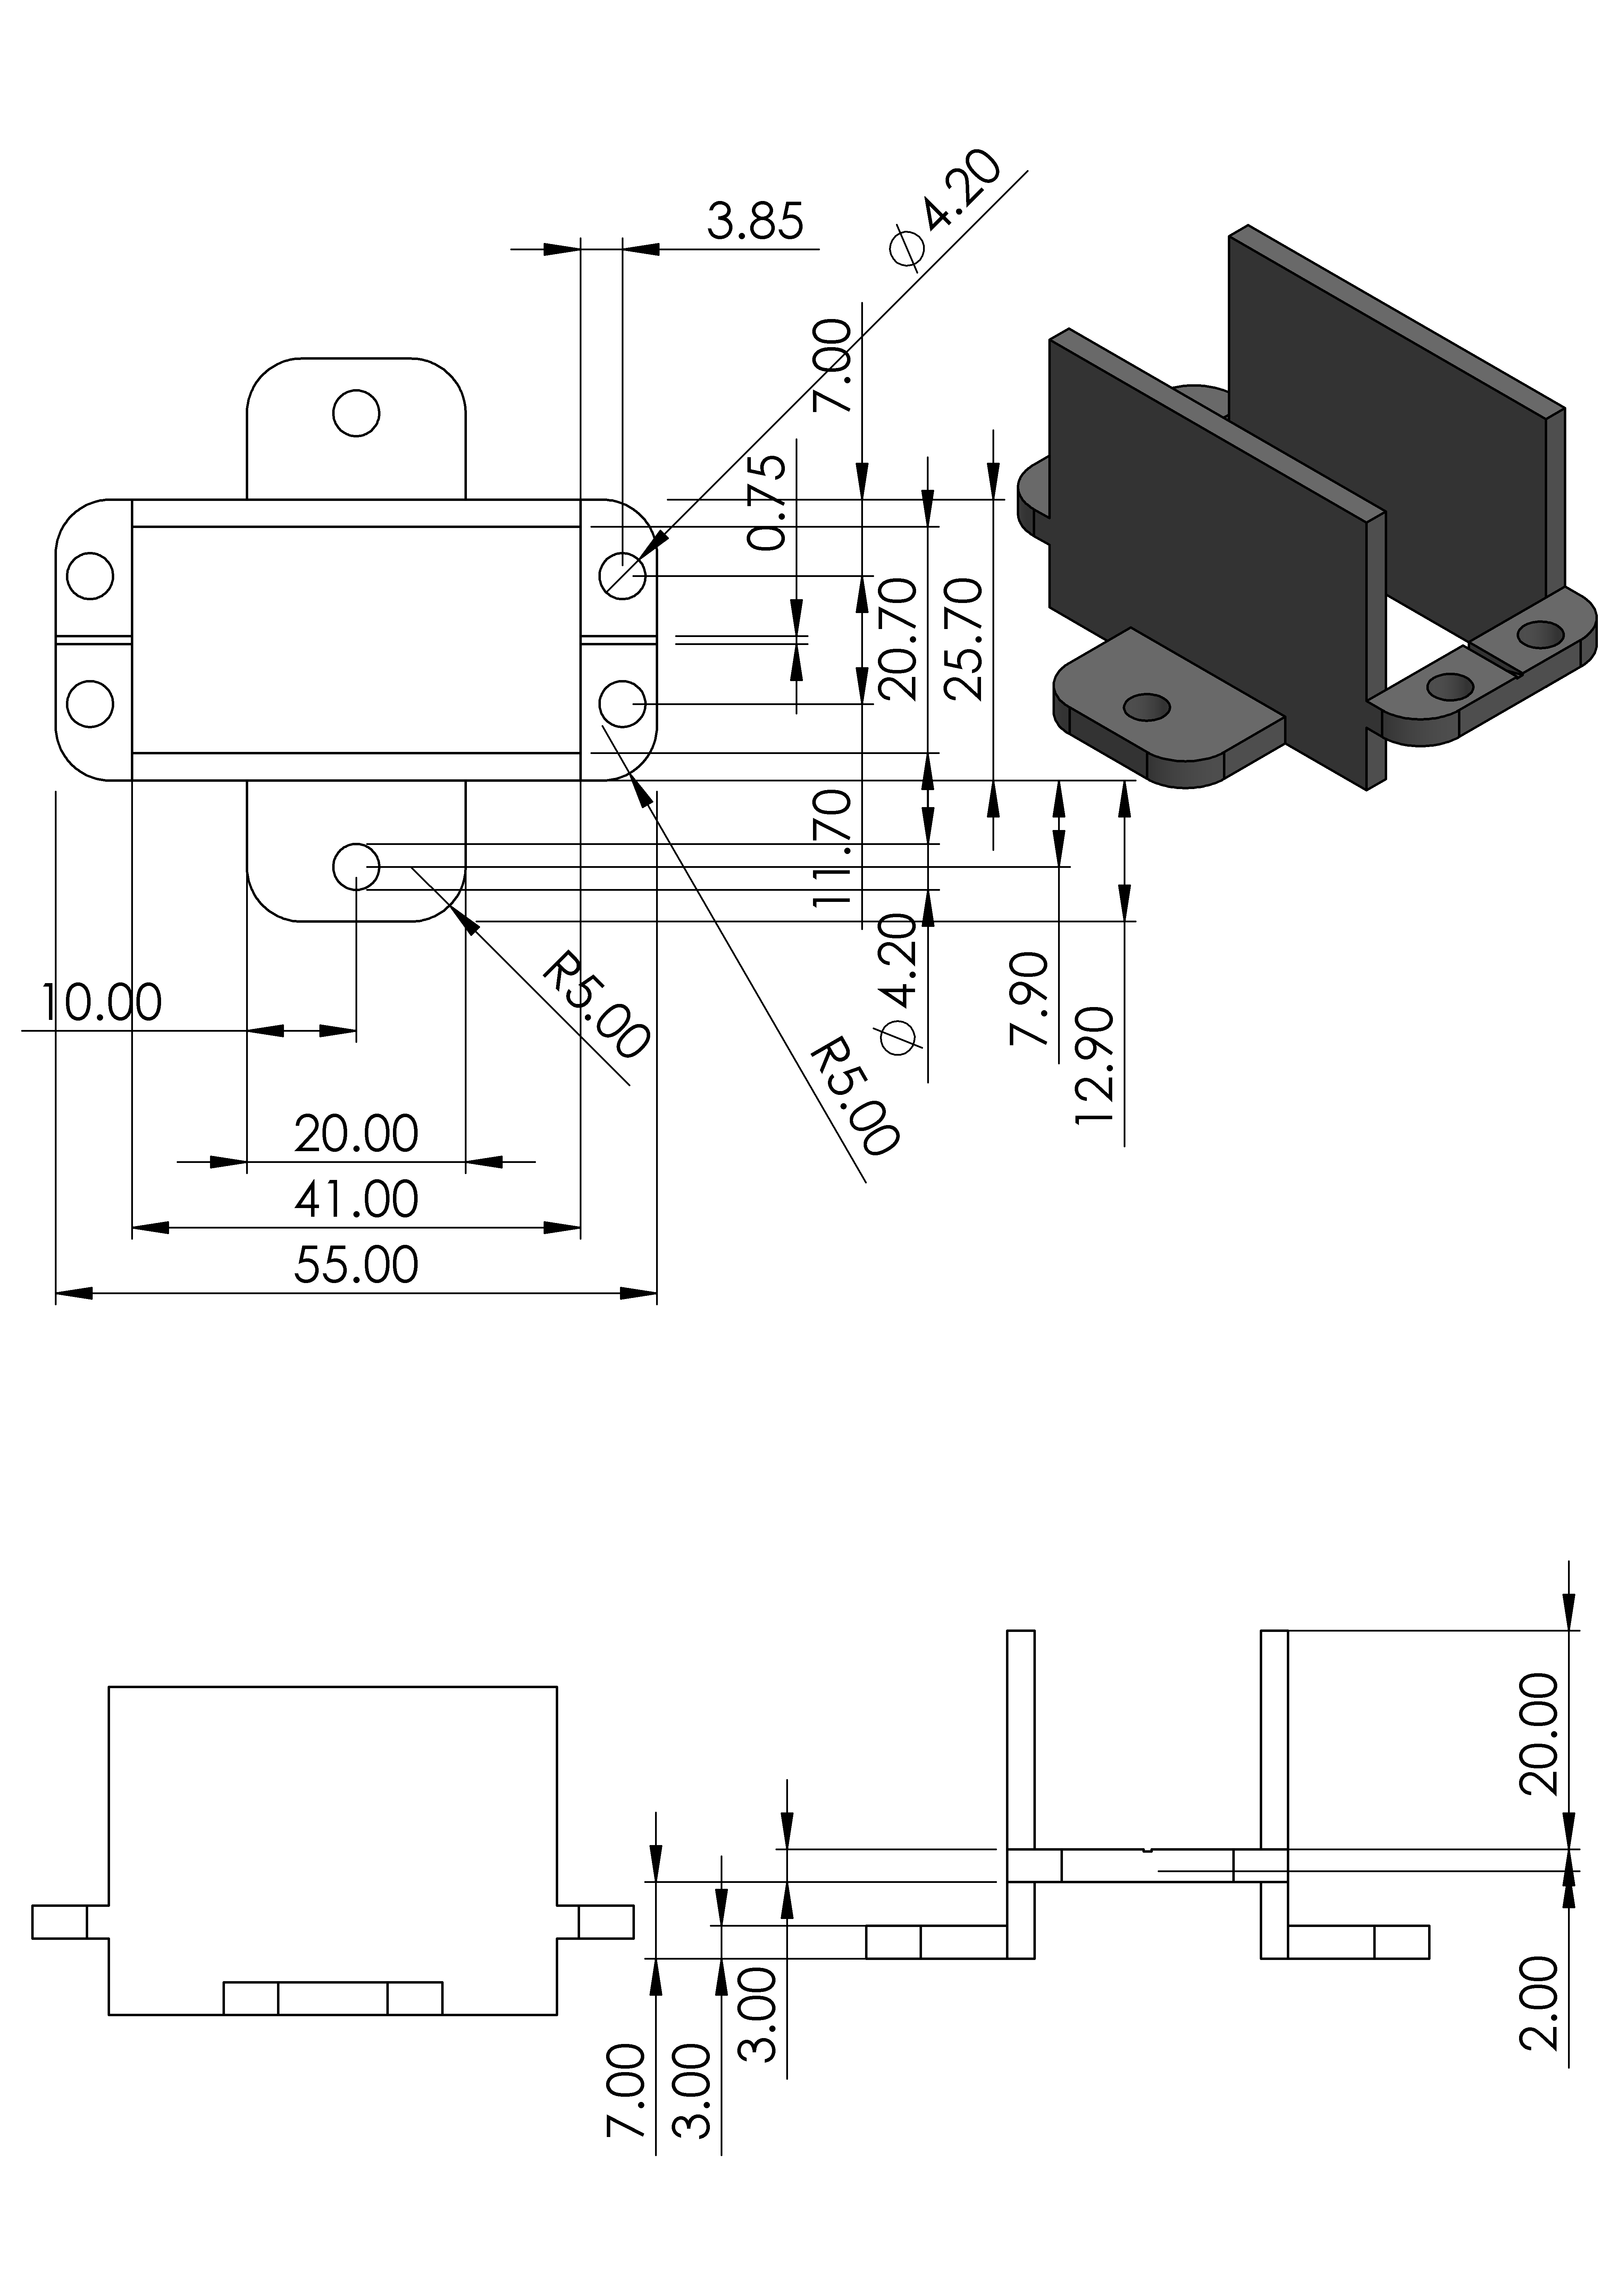
\includegraphics[height=.75\textheight]{Figures/ServoMotorHolder.PNG}
                \caption{Servo motor cage}
                \label{fig:servo_motor_cage}
            \end{figure}
            \par
            \item \textbf{Mounting plate}
            \par
            Figure \ref{fig:servo_motor_mounting_plate} shows the mounting plate for the motor cage. The plate is like a ring with slots. The design allows for rotation without the need to reposition the supporting rods. 
            \par
            \begin{figure}[H]
                \centering
                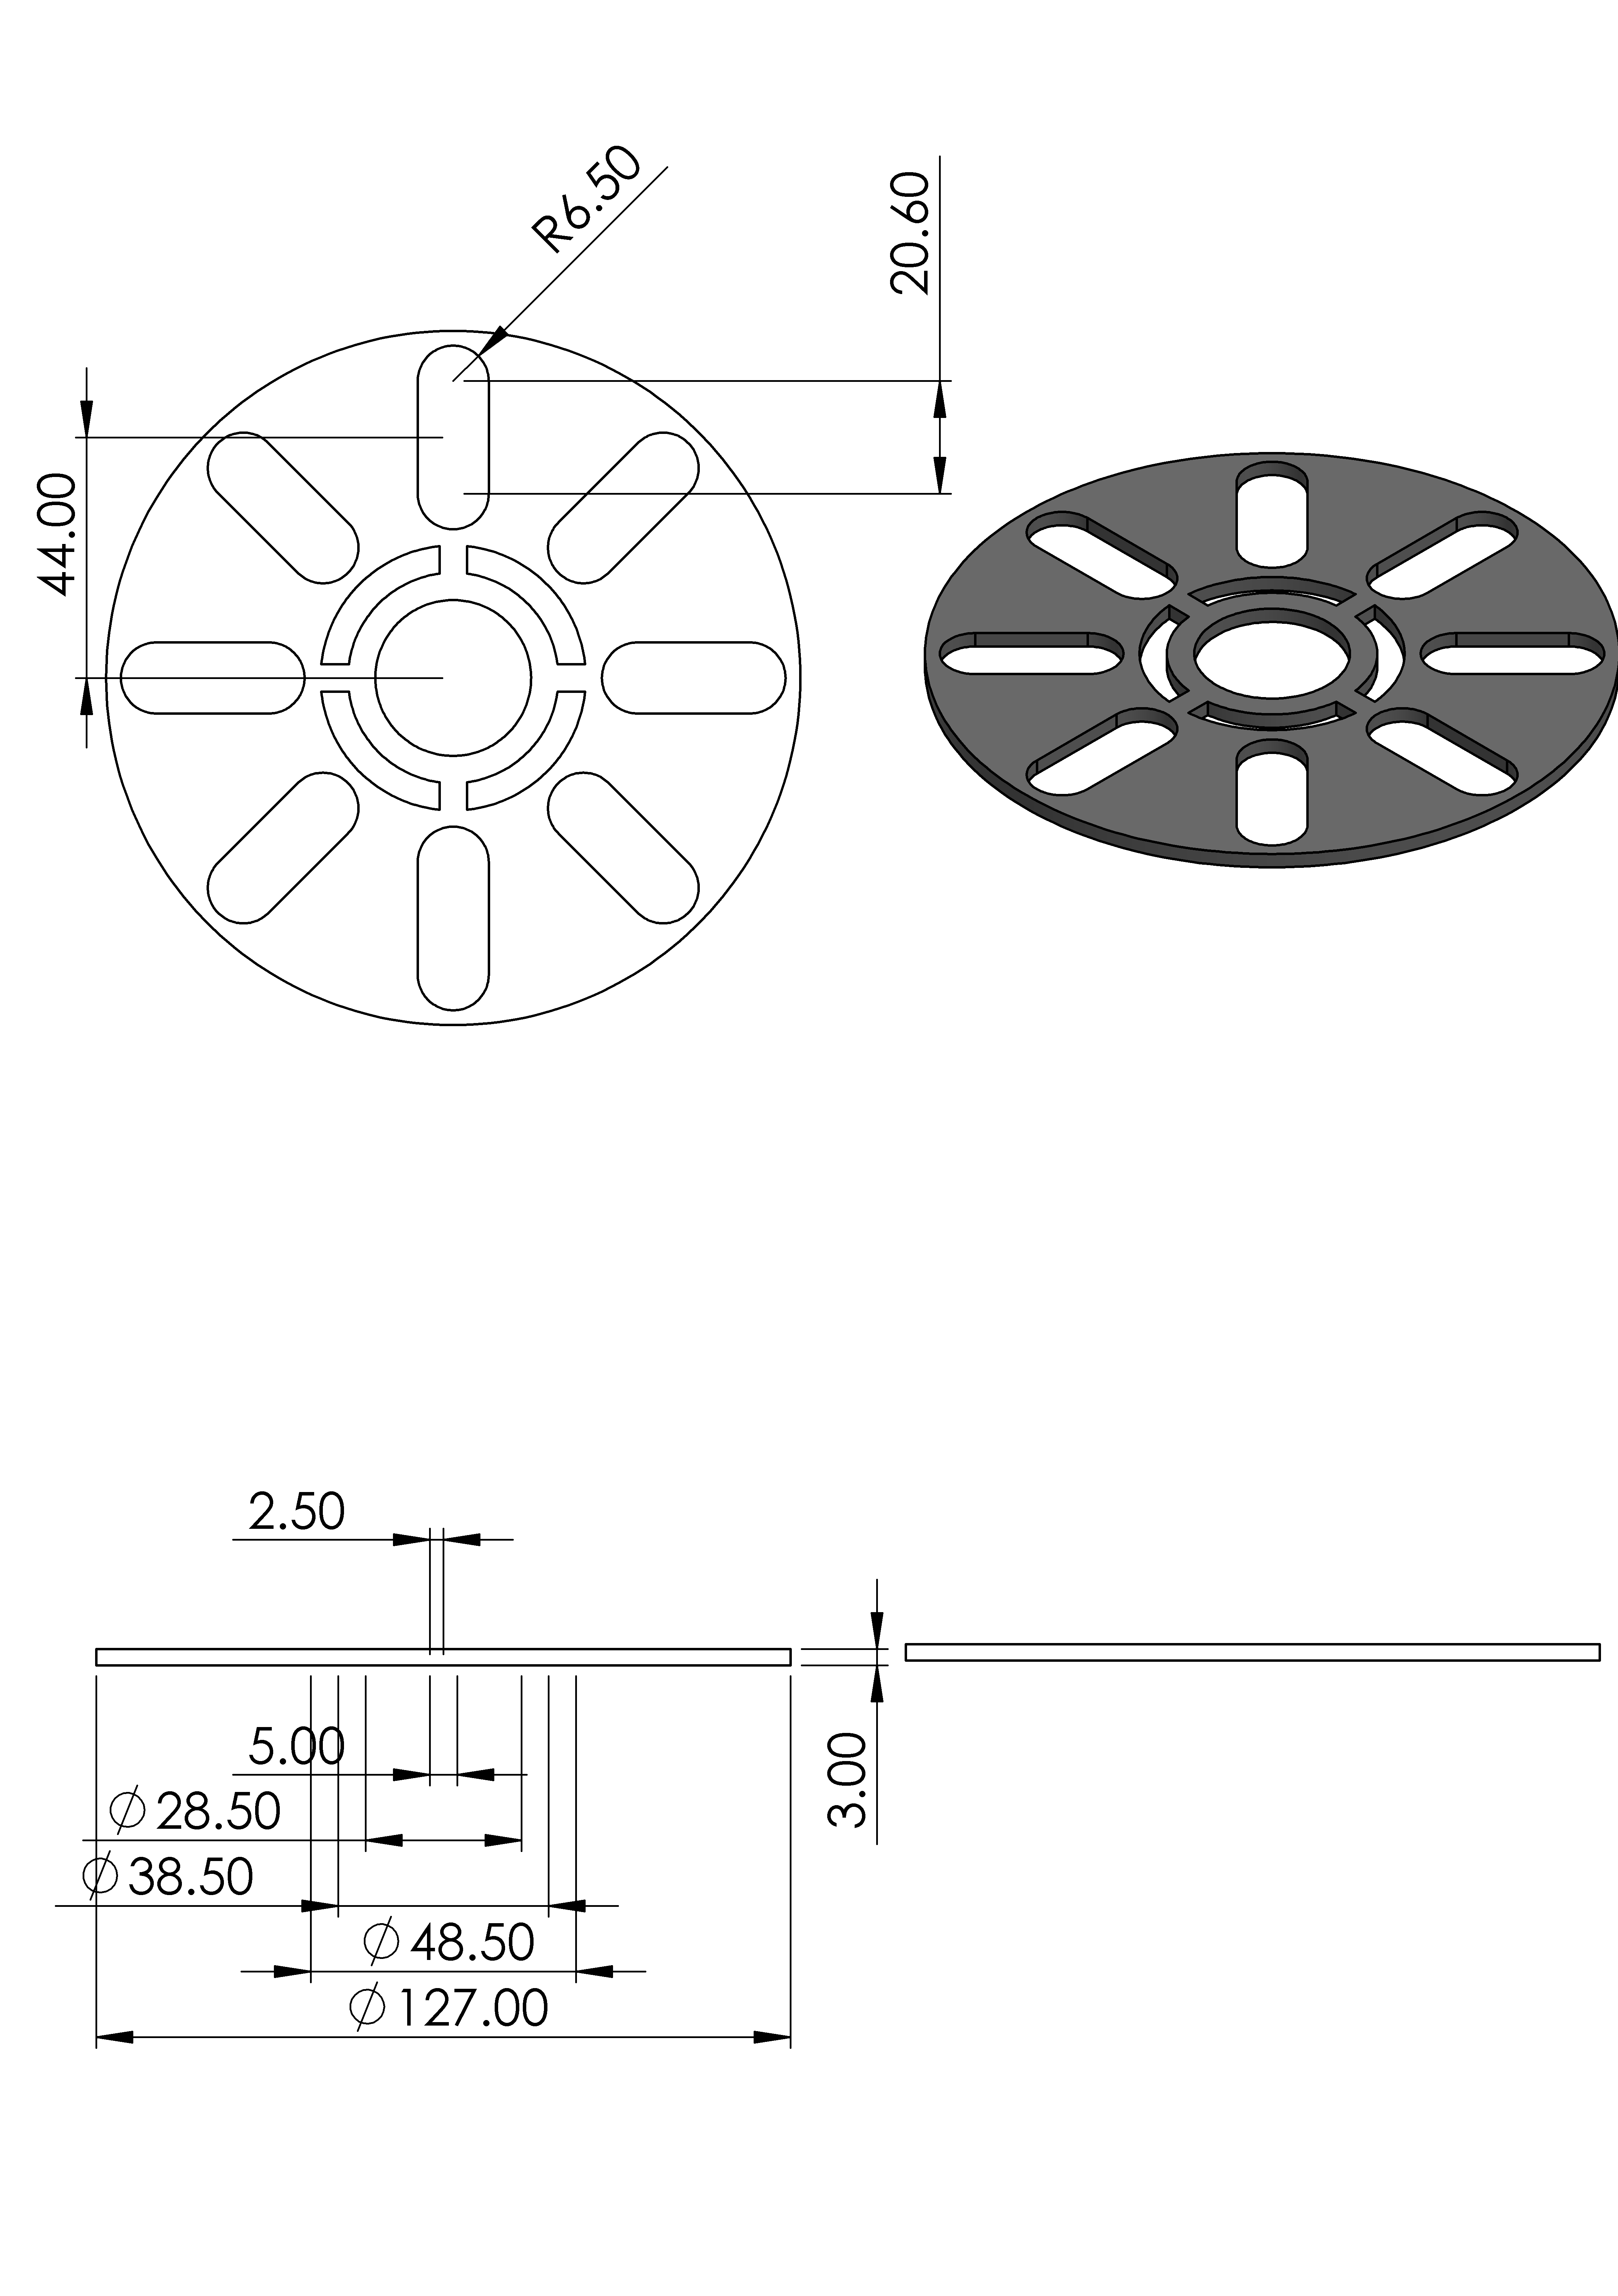
\includegraphics[height=.75\textheight]{Figures/ServoMotorHolderMount.PNG}
                \caption{Servo motor mounting plate}
                \label{fig:servo_motor_mounting_plate}
            \end{figure}
            \par
            \item \textbf{The holder assembly}
            \par
            Figure \ref{fig:servo_motor_mounted_assembly} shows the servo motor cage with the servo motor mounted on the mounting plate. The servo motor assembly can be rotated and translated to reposition the line of rotation of the motor axle. 
            \begin{figure}[H]
                \centering
                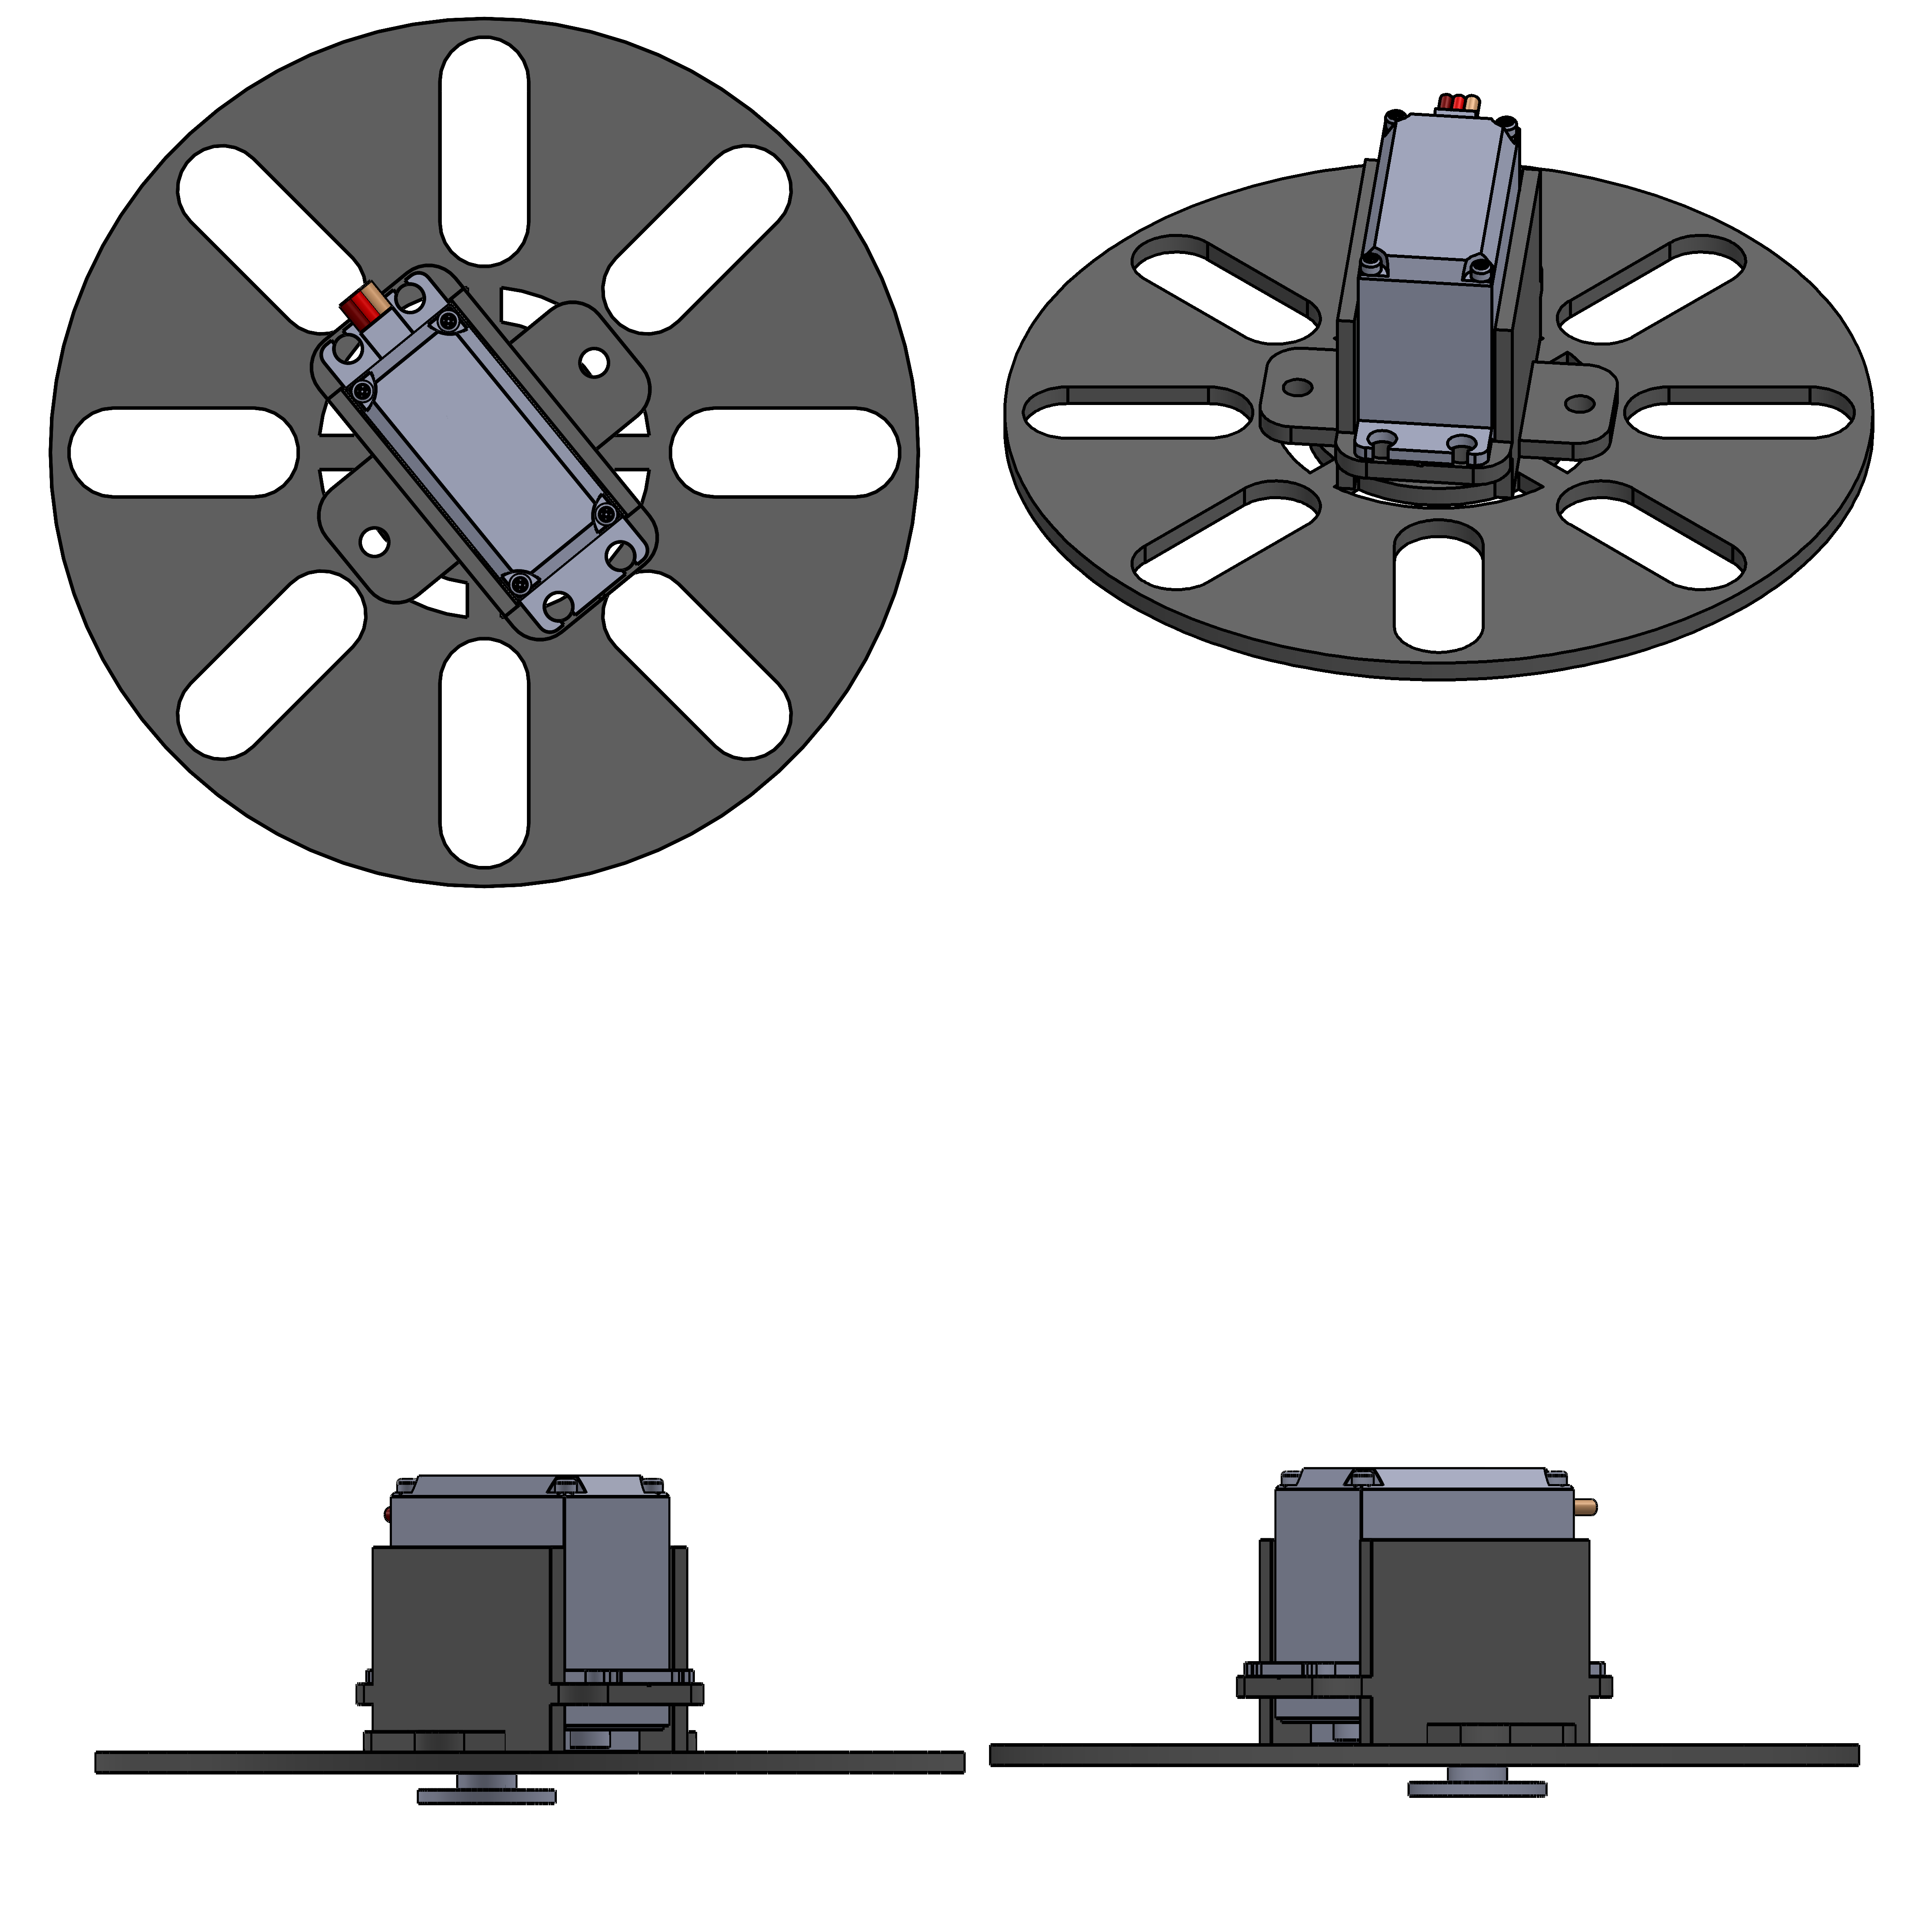
\includegraphics{Figures/ServoMotorMountedAssembly.PNG}
                \caption{Servo motor mounted assembly}
                \label{fig:servo_motor_mounted_assembly}
            \end{figure}
             This design can allow for both rotational and translational adjustments along the slots. However, it is complex and require a lot of fasteners.
         \end{itemize}
         \item A combination of spur gears to always translate the line of rotation of the motor axle to a fixed line of rotation no matter the orientation of the motor.
         \clearpage
         \textbf{Designs with the spur gears approach}
         \par
          \begin{itemize}
              \item \textbf{Spur gears}
              \par
              Spur gear shown in Figure \ref{fig:spur_gear} translates the line of rotation by 5.75mm in any orientation of the servo to a fixed centre line.
              \begin{figure}[H]
                  \centering
                  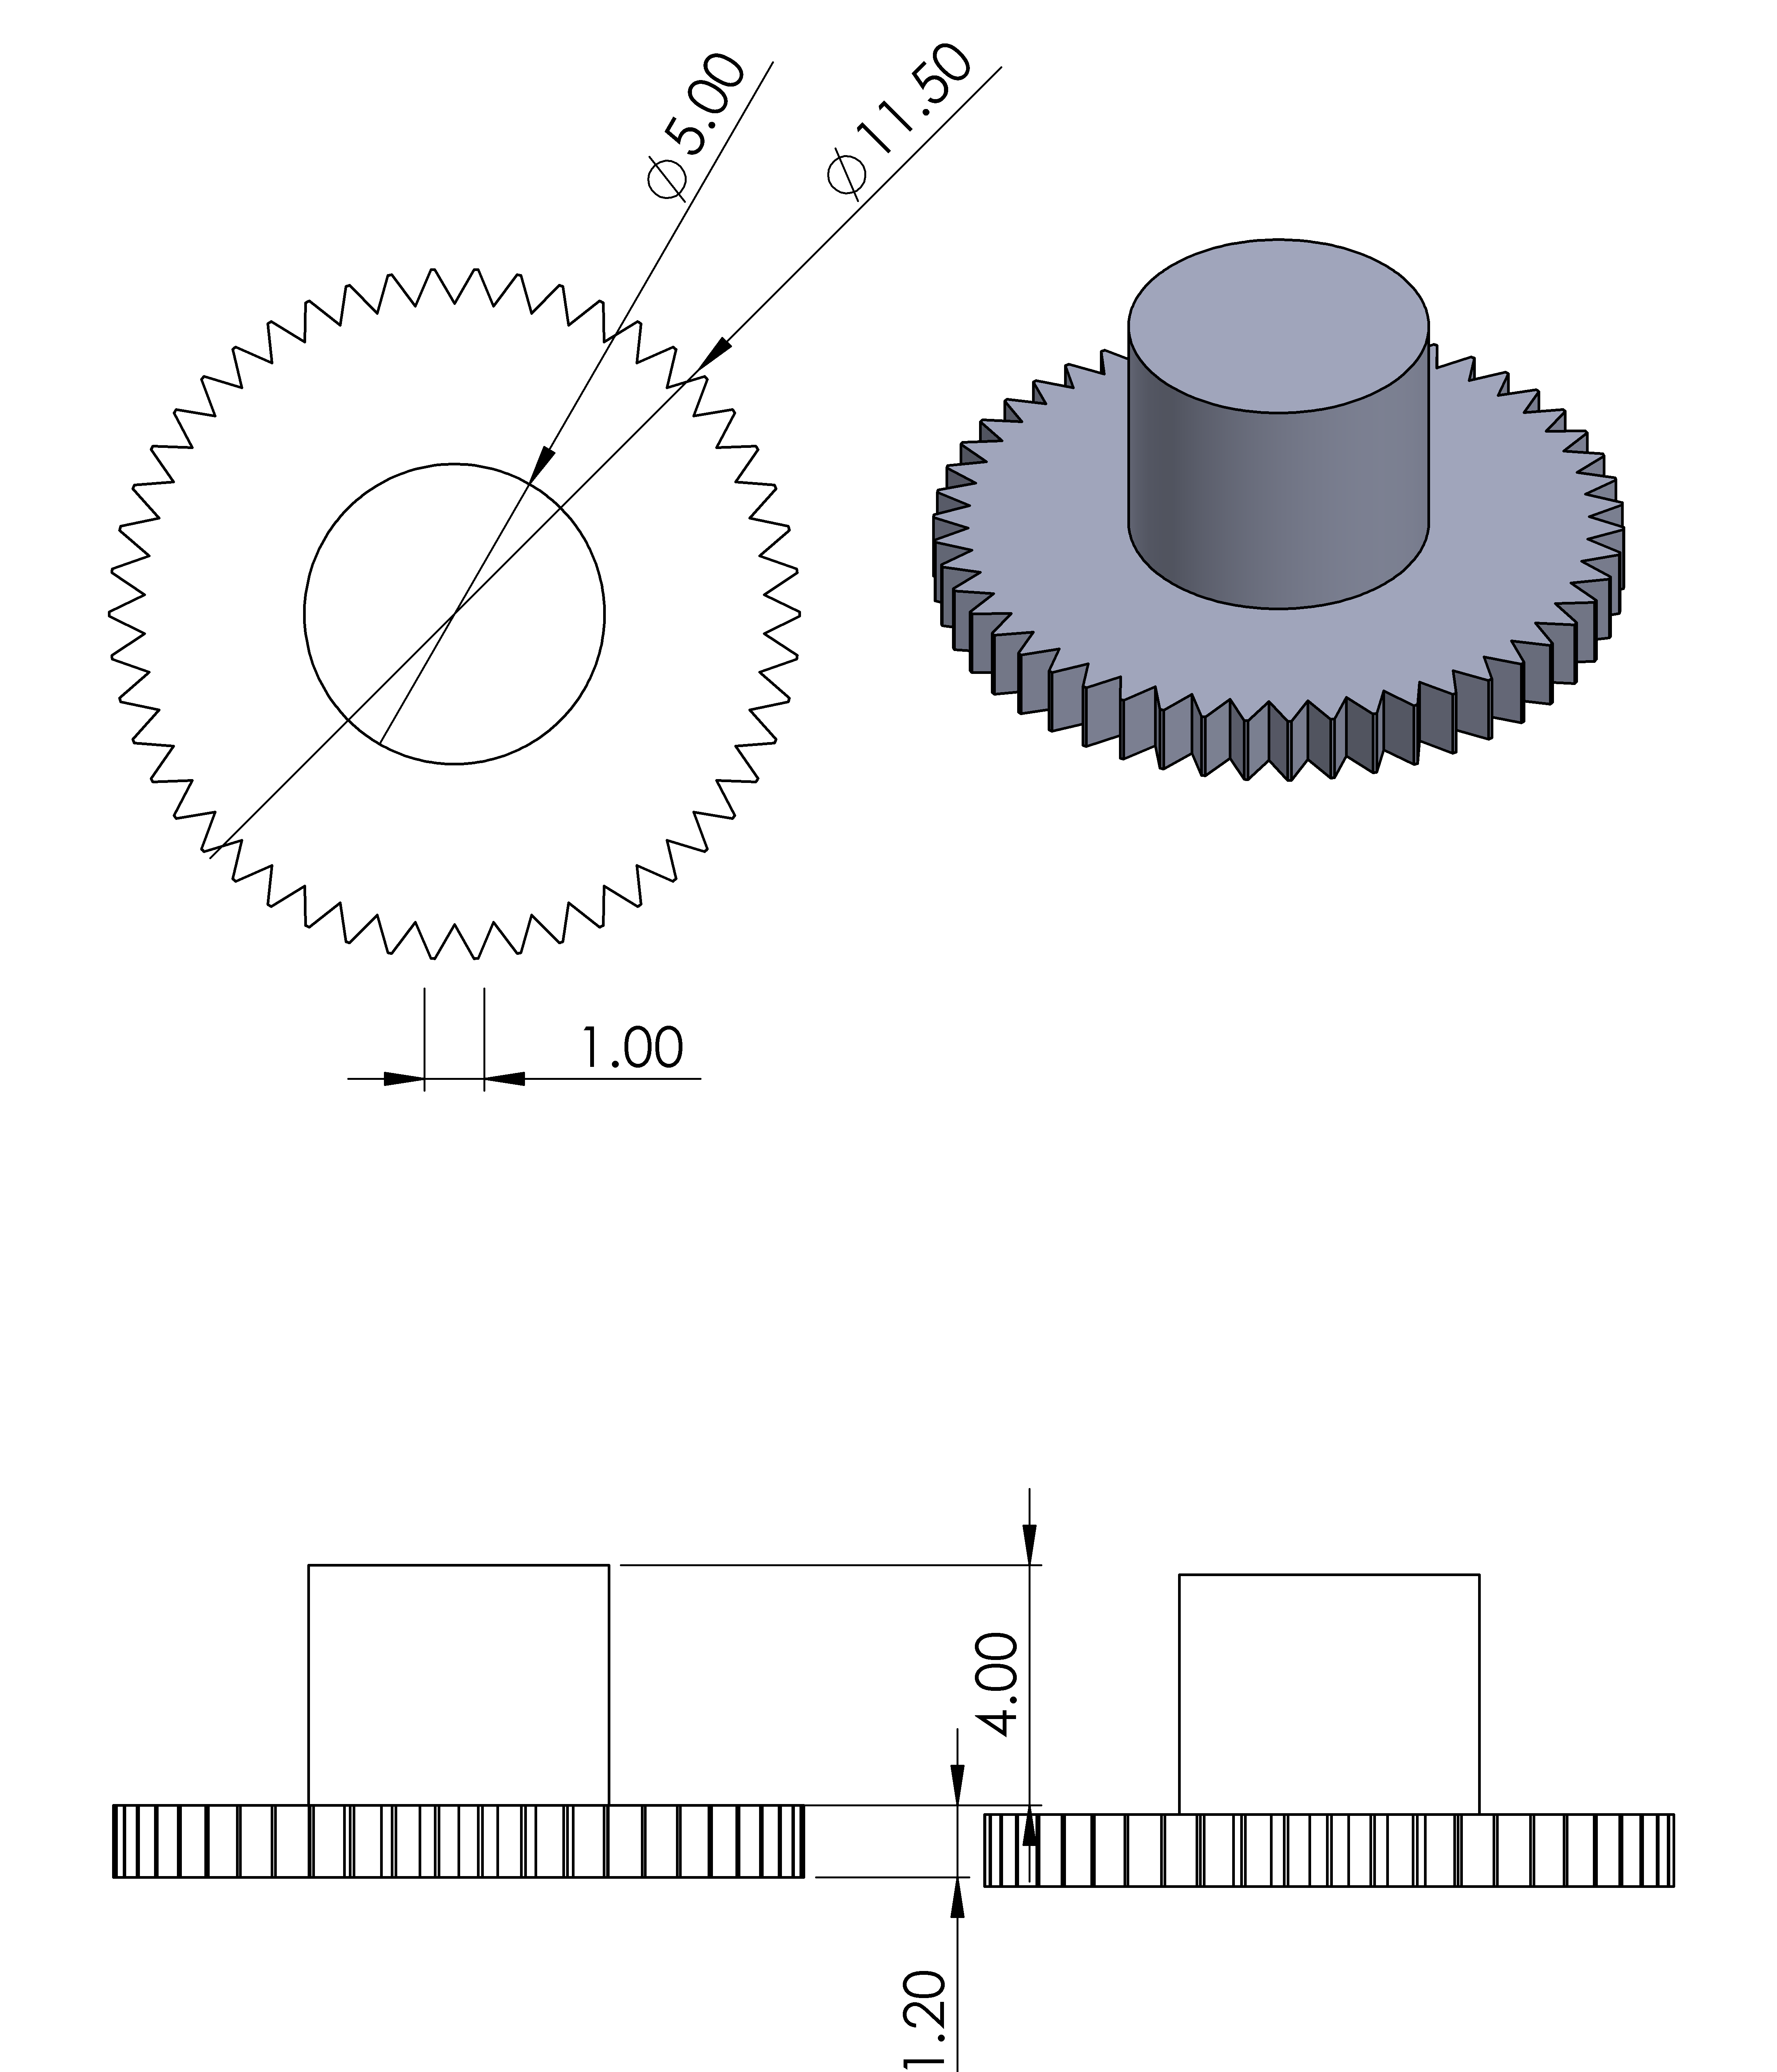
\includegraphics{Figures/SpurGear1.PNG}
                  \caption{Spur gear}
                  \label{fig:spur_gear}
              \end{figure}
              \par 
              \item  \textbf{Servo motor-spur gear assembly}
              \par
              Figure \ref{fig:servo_motor_with_spur_gears} shows the spur gear translation system assembled with the servo motor.
              \begin{figure}[H]
                  \centering
                  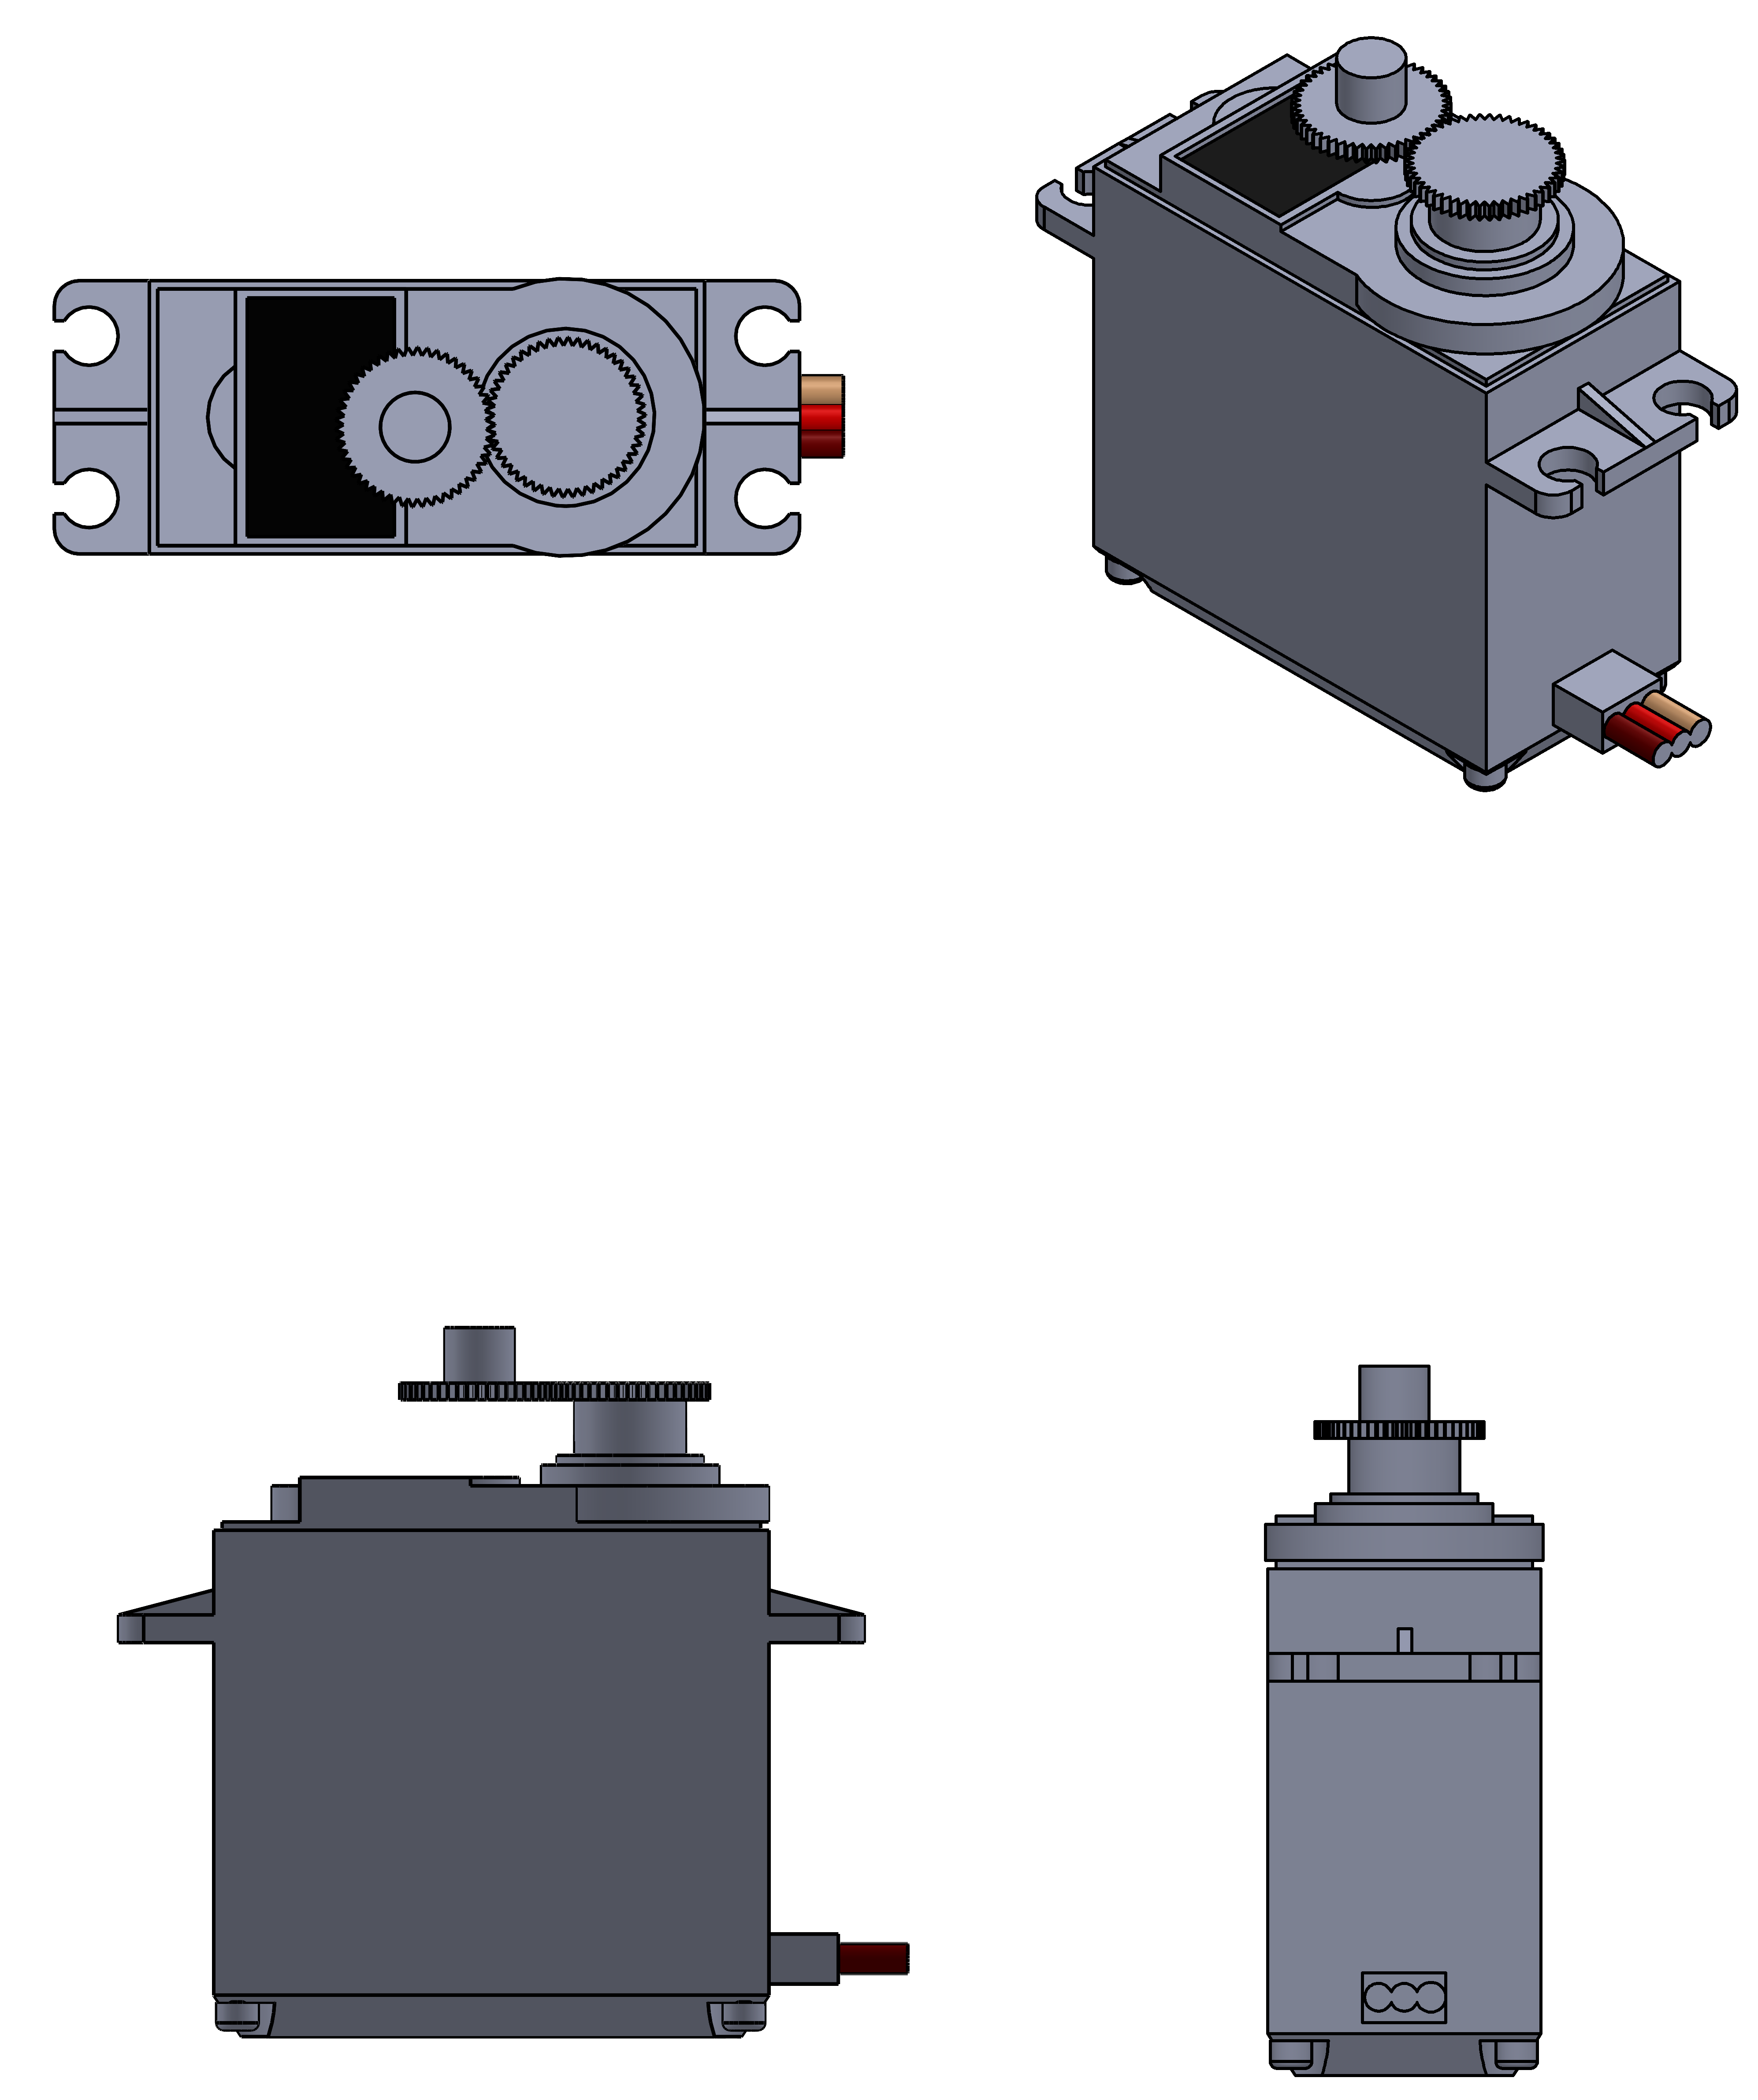
\includegraphics{Figures/ServoMotorWithSpurGears.PNG}
                  \caption{Servo motor with spur gears}
                  \label{fig:servo_motor_with_spur_gears}
              \end{figure}
              This design is quite simpler than the first approach. The design considerations are few and can produce even finer translations in the scale of the spur gear pitch($1 mm$). However, the main challenge with this design is the durability of spur gears made of PLA material since servo motors tend to have a high starting torque. This will almost necessitate the replacement of the gears after every two or three experiments.  
          \end{itemize}
     \end{enumerate}
     \par
     Between the two mounting designs described, the first options had more merits than the second option. It might require more material to produce it but at least it is only for one time unlike with second option where the gears are to be replaced after every two or three times in operation.
     \par 
     \item \textbf{Mounting rod}
     \par
     Two of the rod shown in figure \ref{fig:mounting_rods} are used to support the mounted servo motor assembly on the ball valve. The design was such that it allowed for fasteners on both sides: at one end, to fasten the servo motor assembly after alignment and at the other end, to fasten the whole flow control unit on the main discharge pipe.
     \par
     The protrusion of its surface eliminates the need for another fastener. 
      \begin{figure}[H]
          \centering
          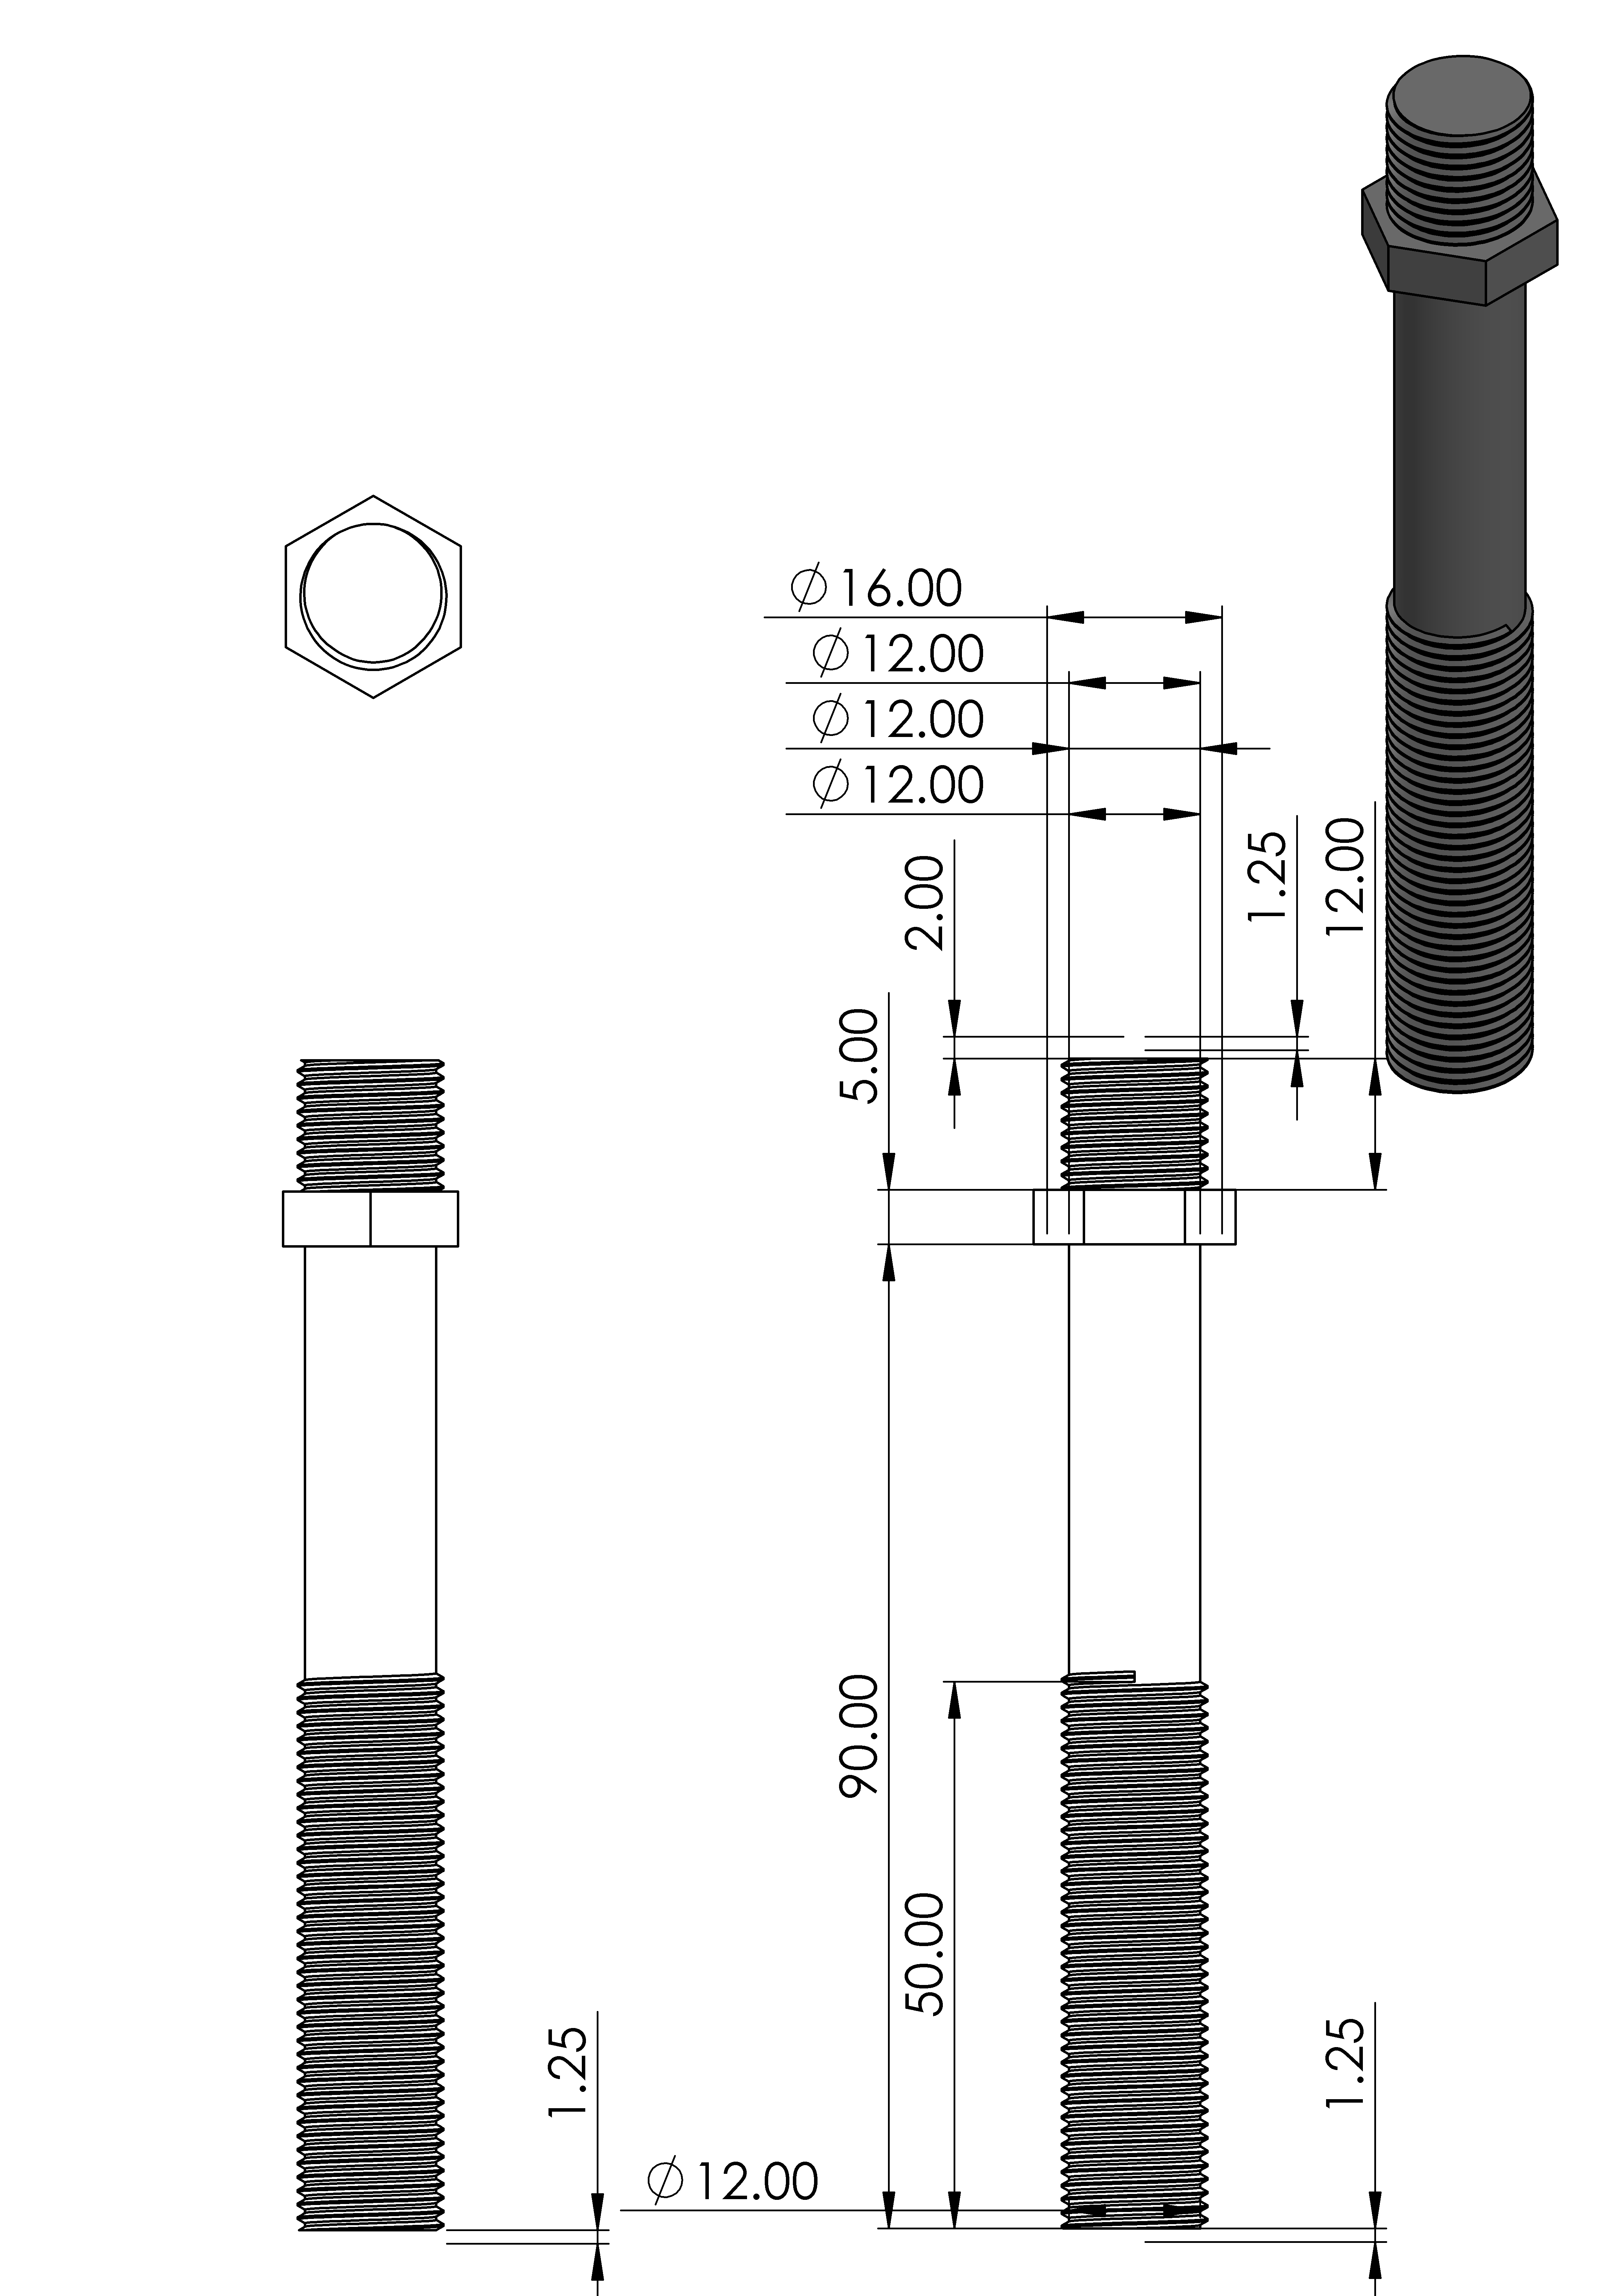
\includegraphics[height=.75\textheight]{Figures/ServoMotorMountRods.PNG}
          \caption{Mounting rods}
          \label{fig:mounting_rods}
      \end{figure}
      \par
    \item \textbf{Interface}
    \par
    The interface shown in Figure \ref{fig:interface2} is an improvement from the interface that was used with the stepper motor. This design is minimalistic and requires a lesser volume of material to produce. In addition, it also has provisions(hooks) to allow for even finer adjustments in the first approach for mounting the servo motor.
    \begin{figure}[H]
        \centering
        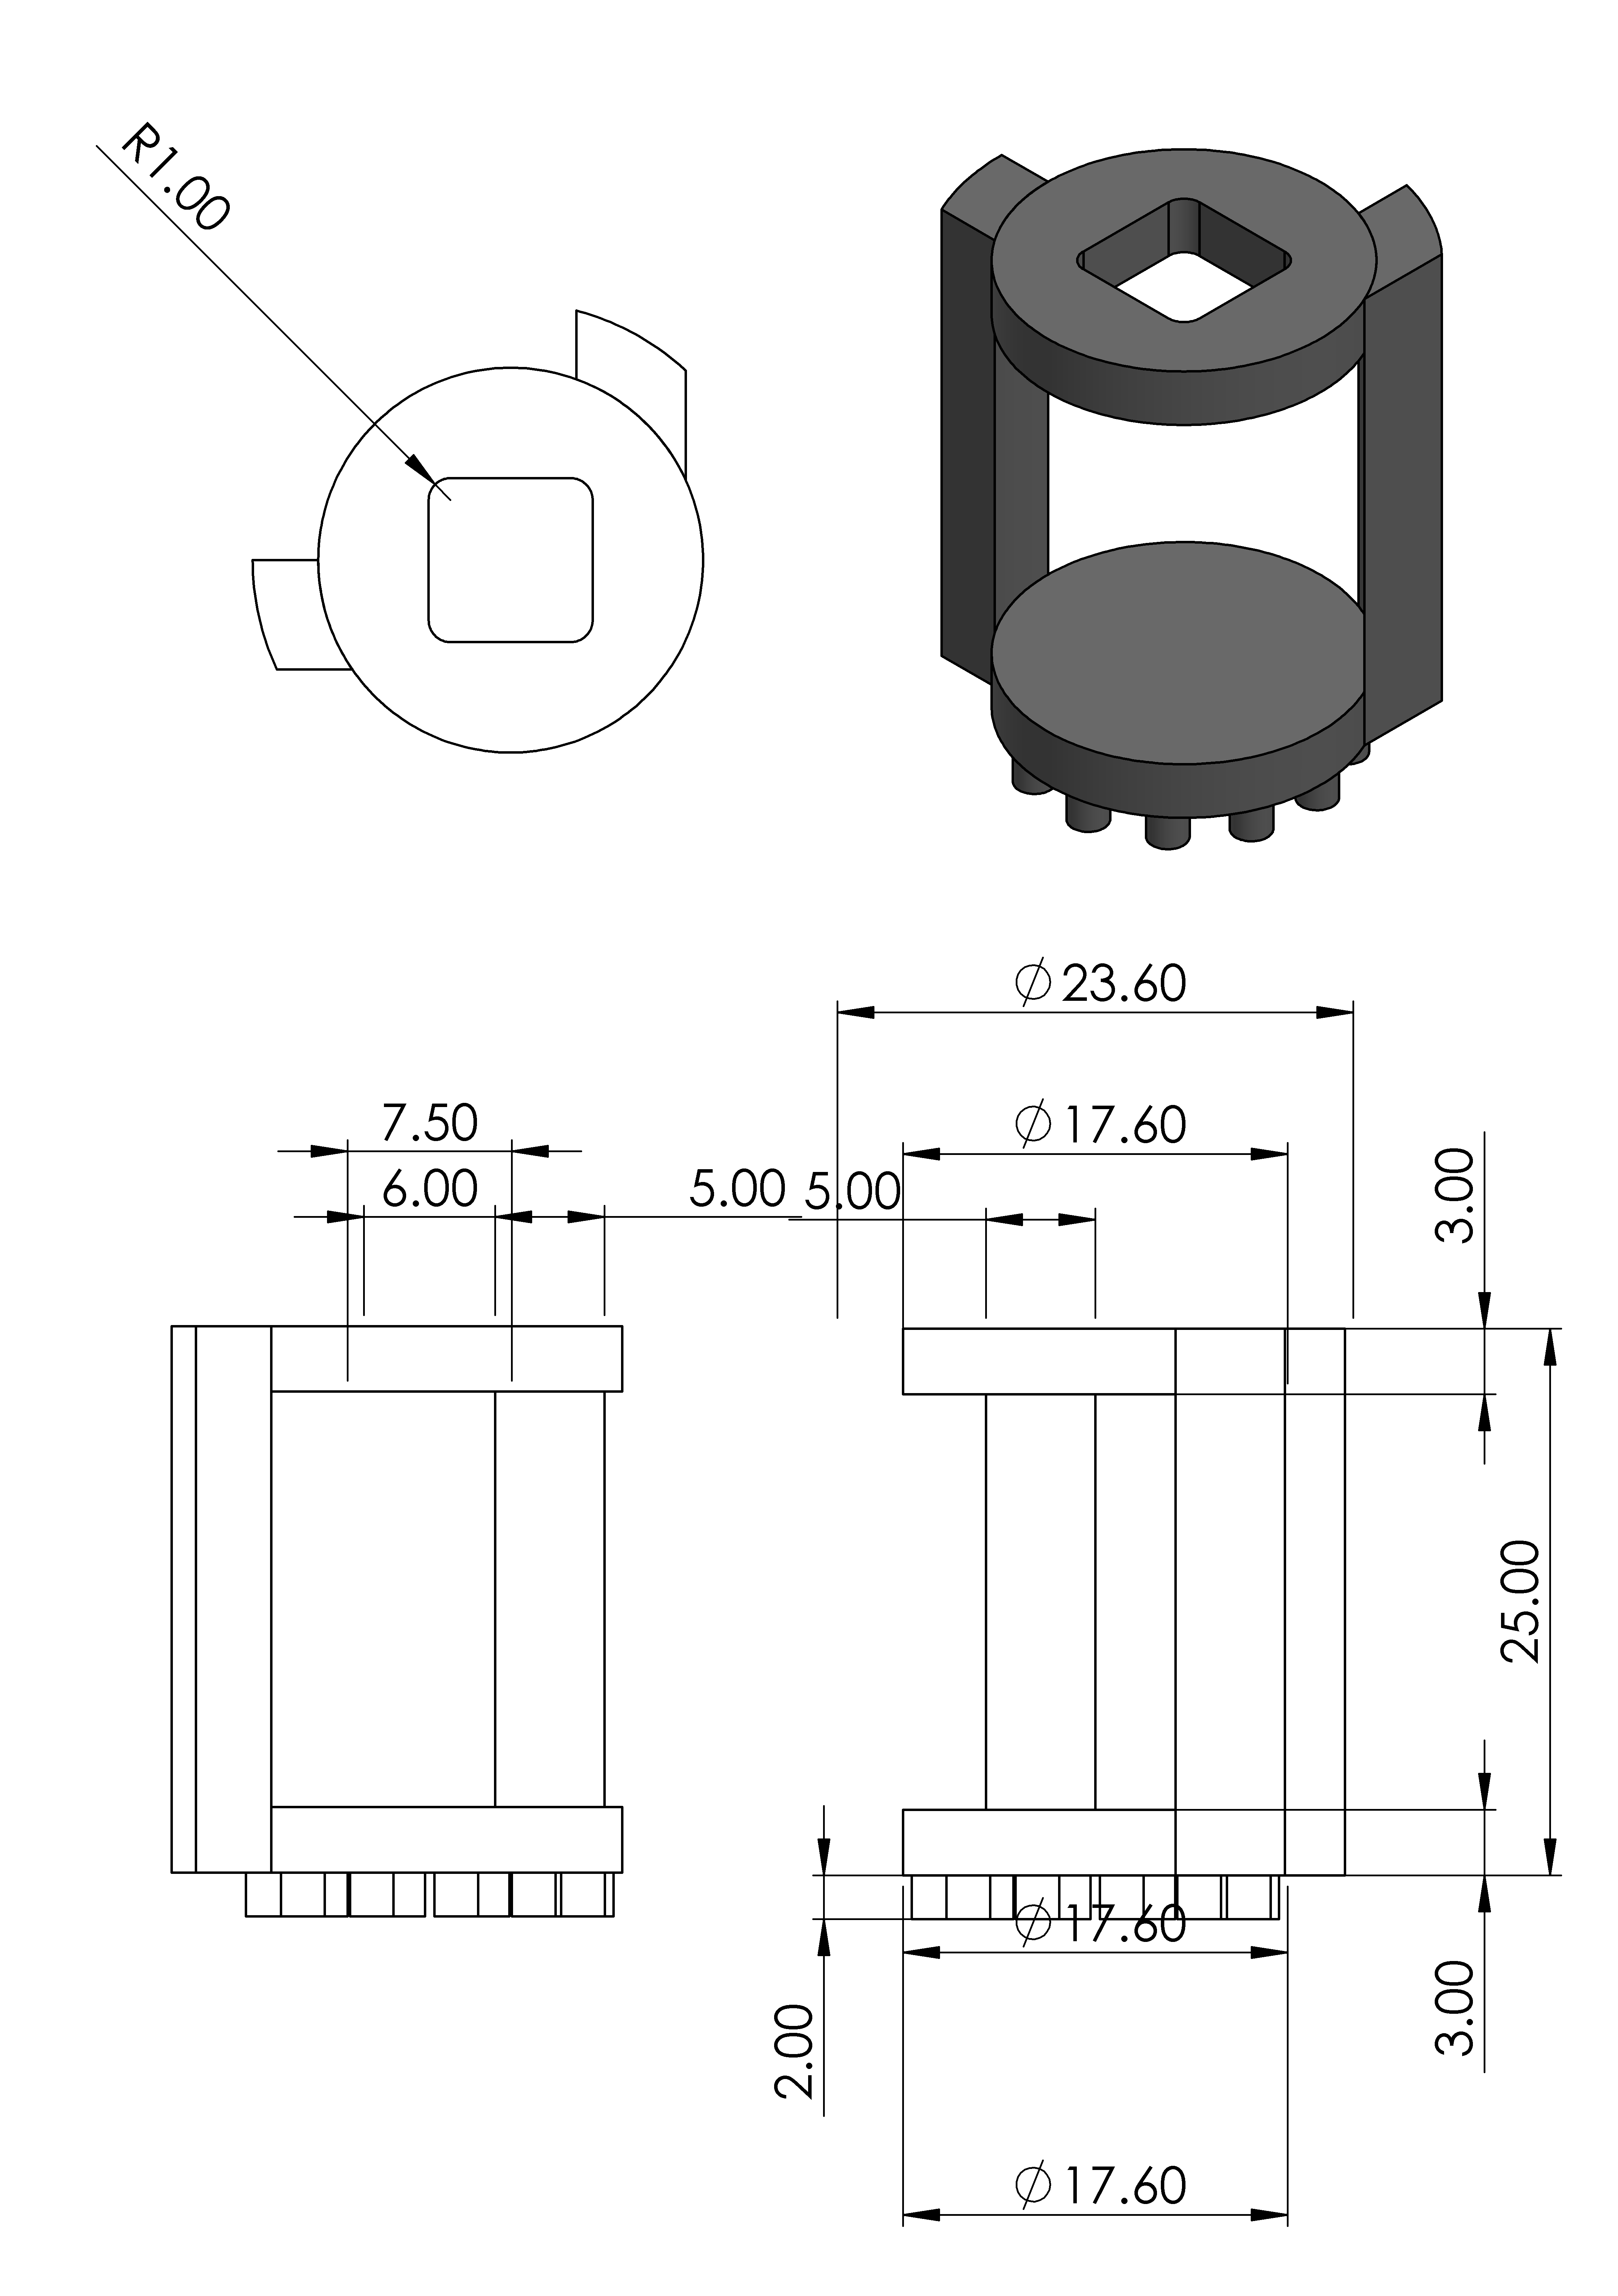
\includegraphics[height=.5\textheight]{Figures/Interface2.PNG}
        \caption{Interface}
        \label{fig:interface2}
    \end{figure}
    \par
    \item \textbf{Straps}
    \par
    Serrated straps shown in \ref{fig:two_rail_serrated_straps} are also an improvement on the straps used in the stepper motor approach. The serration provide more grip on the discharge pipe. It can also support more load. The sizing and dimensioning was guided by the existing ball valve casing.
    \begin{figure}[H]
        \centering
        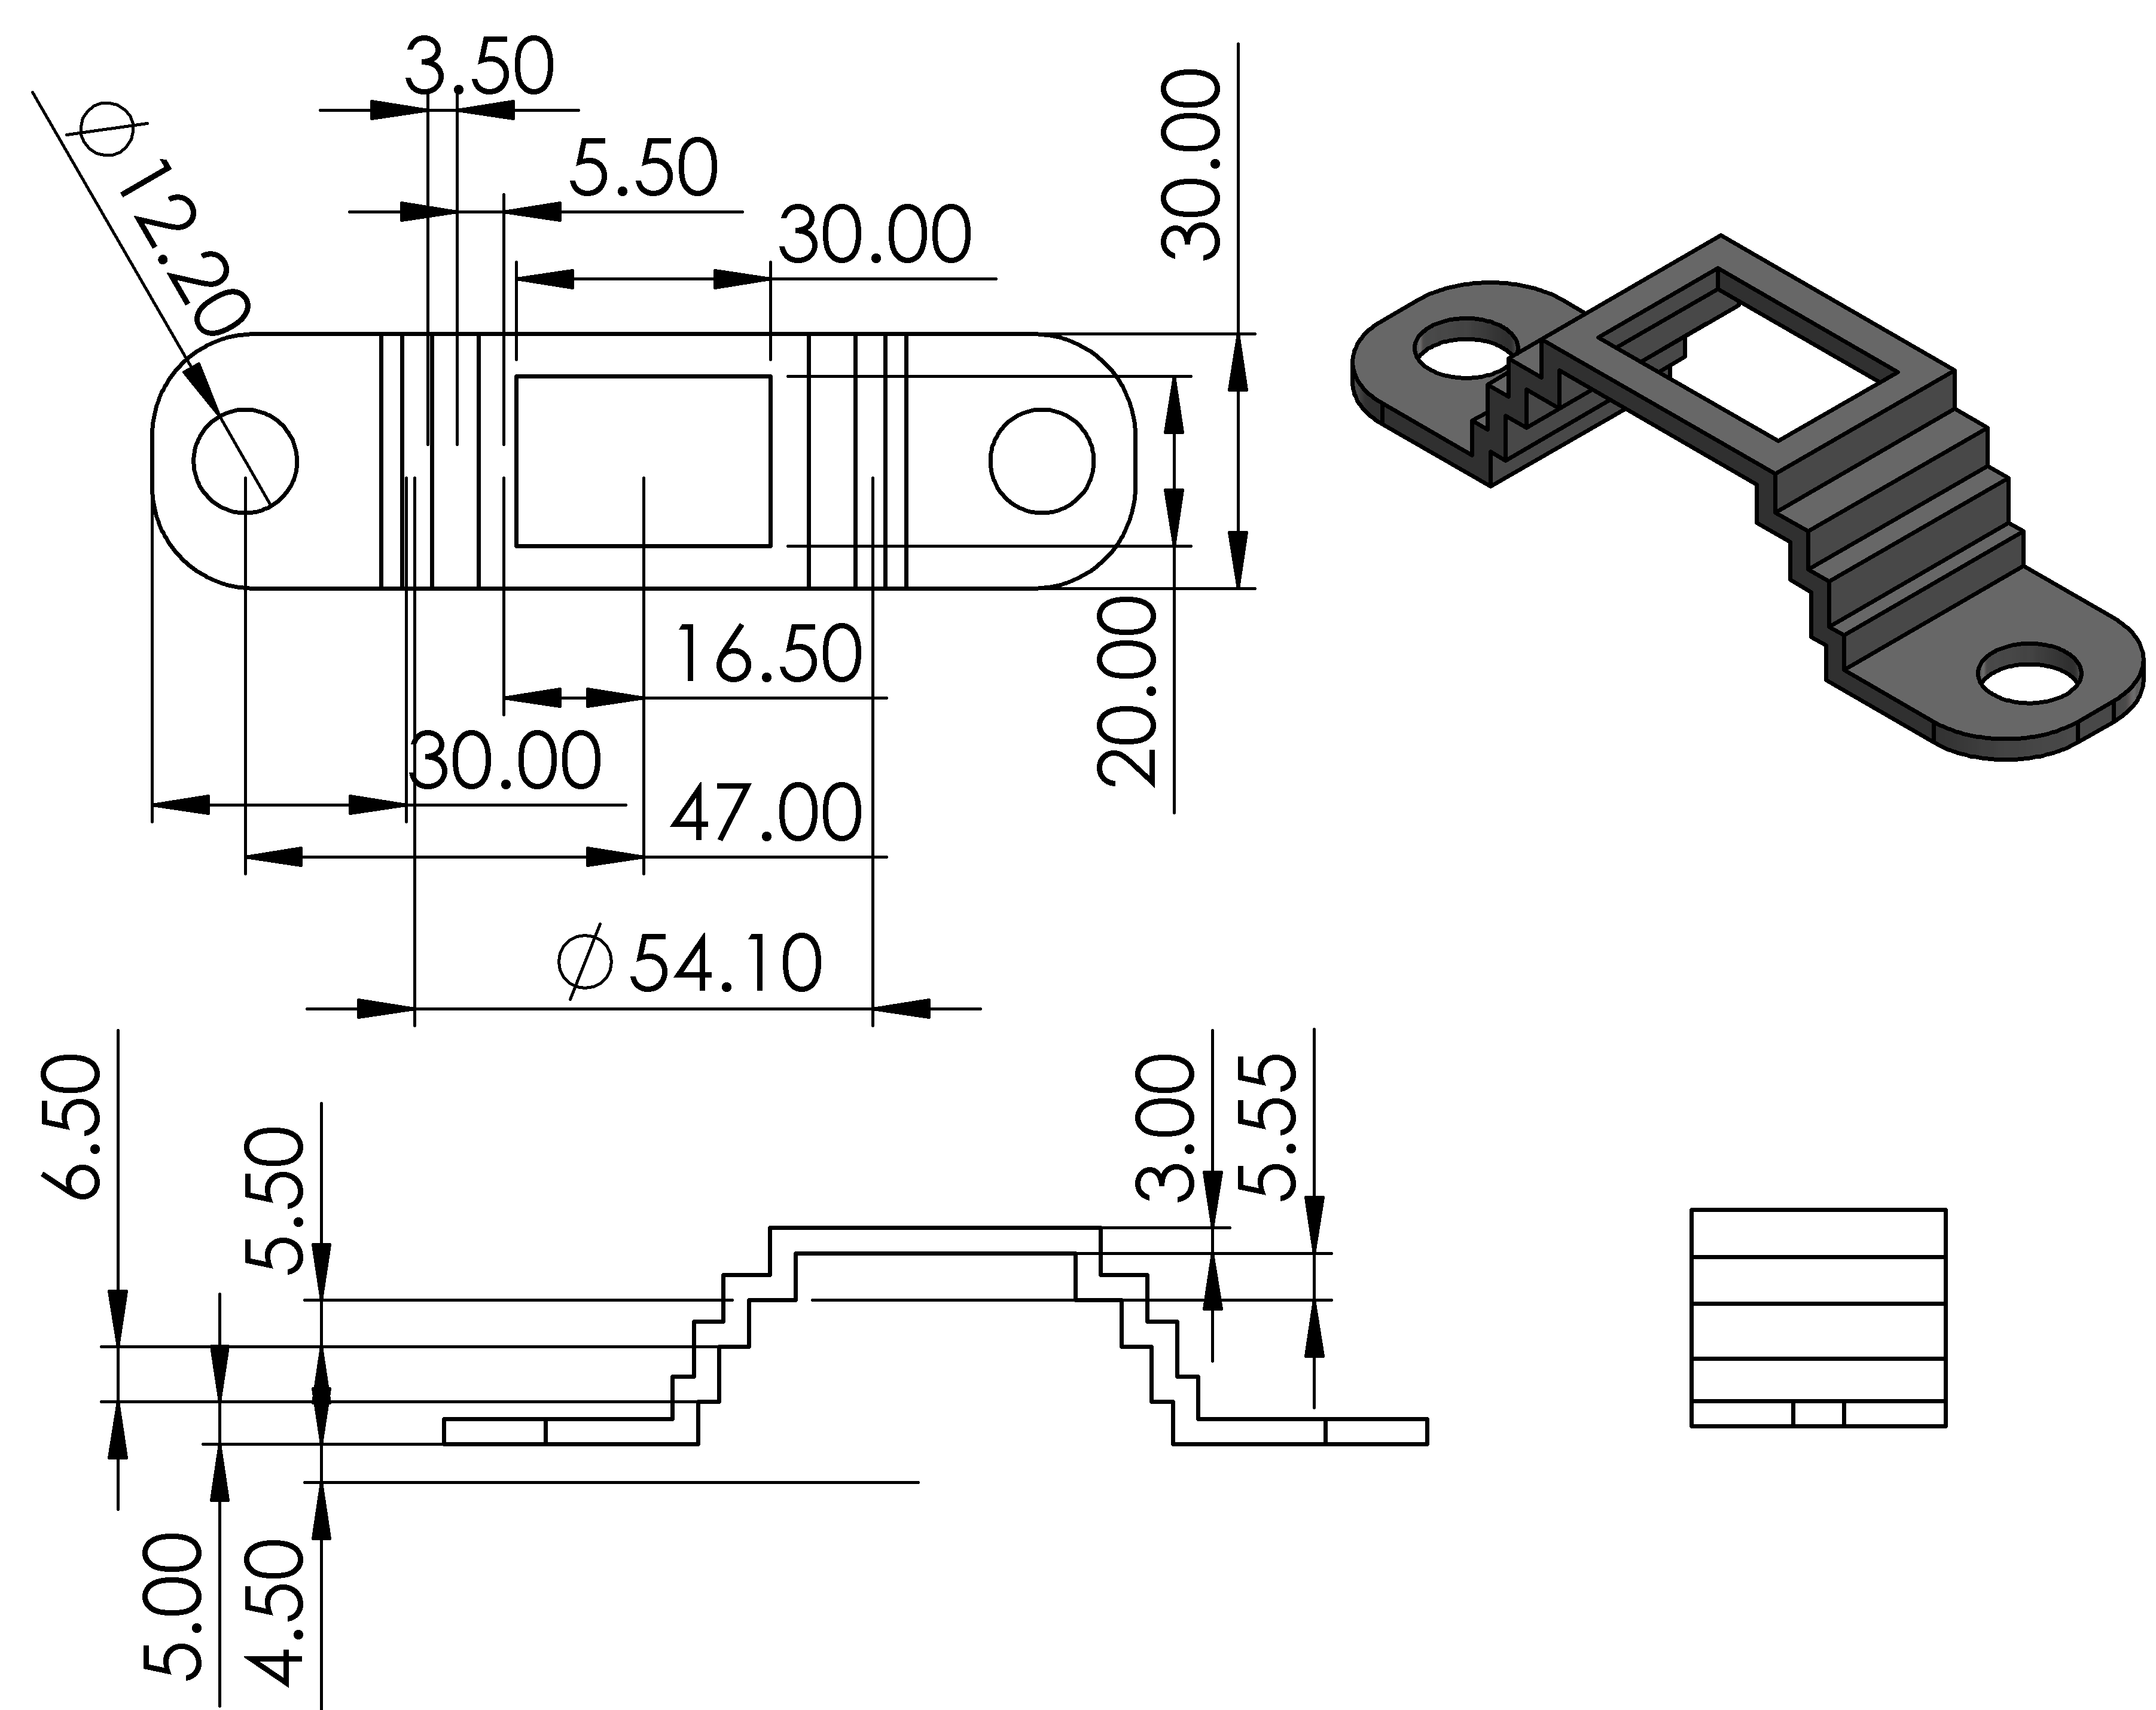
\includegraphics[height=.45\textheight]{Figures/twoRailStrapsTop.PNG}
        \caption{Top strap}
        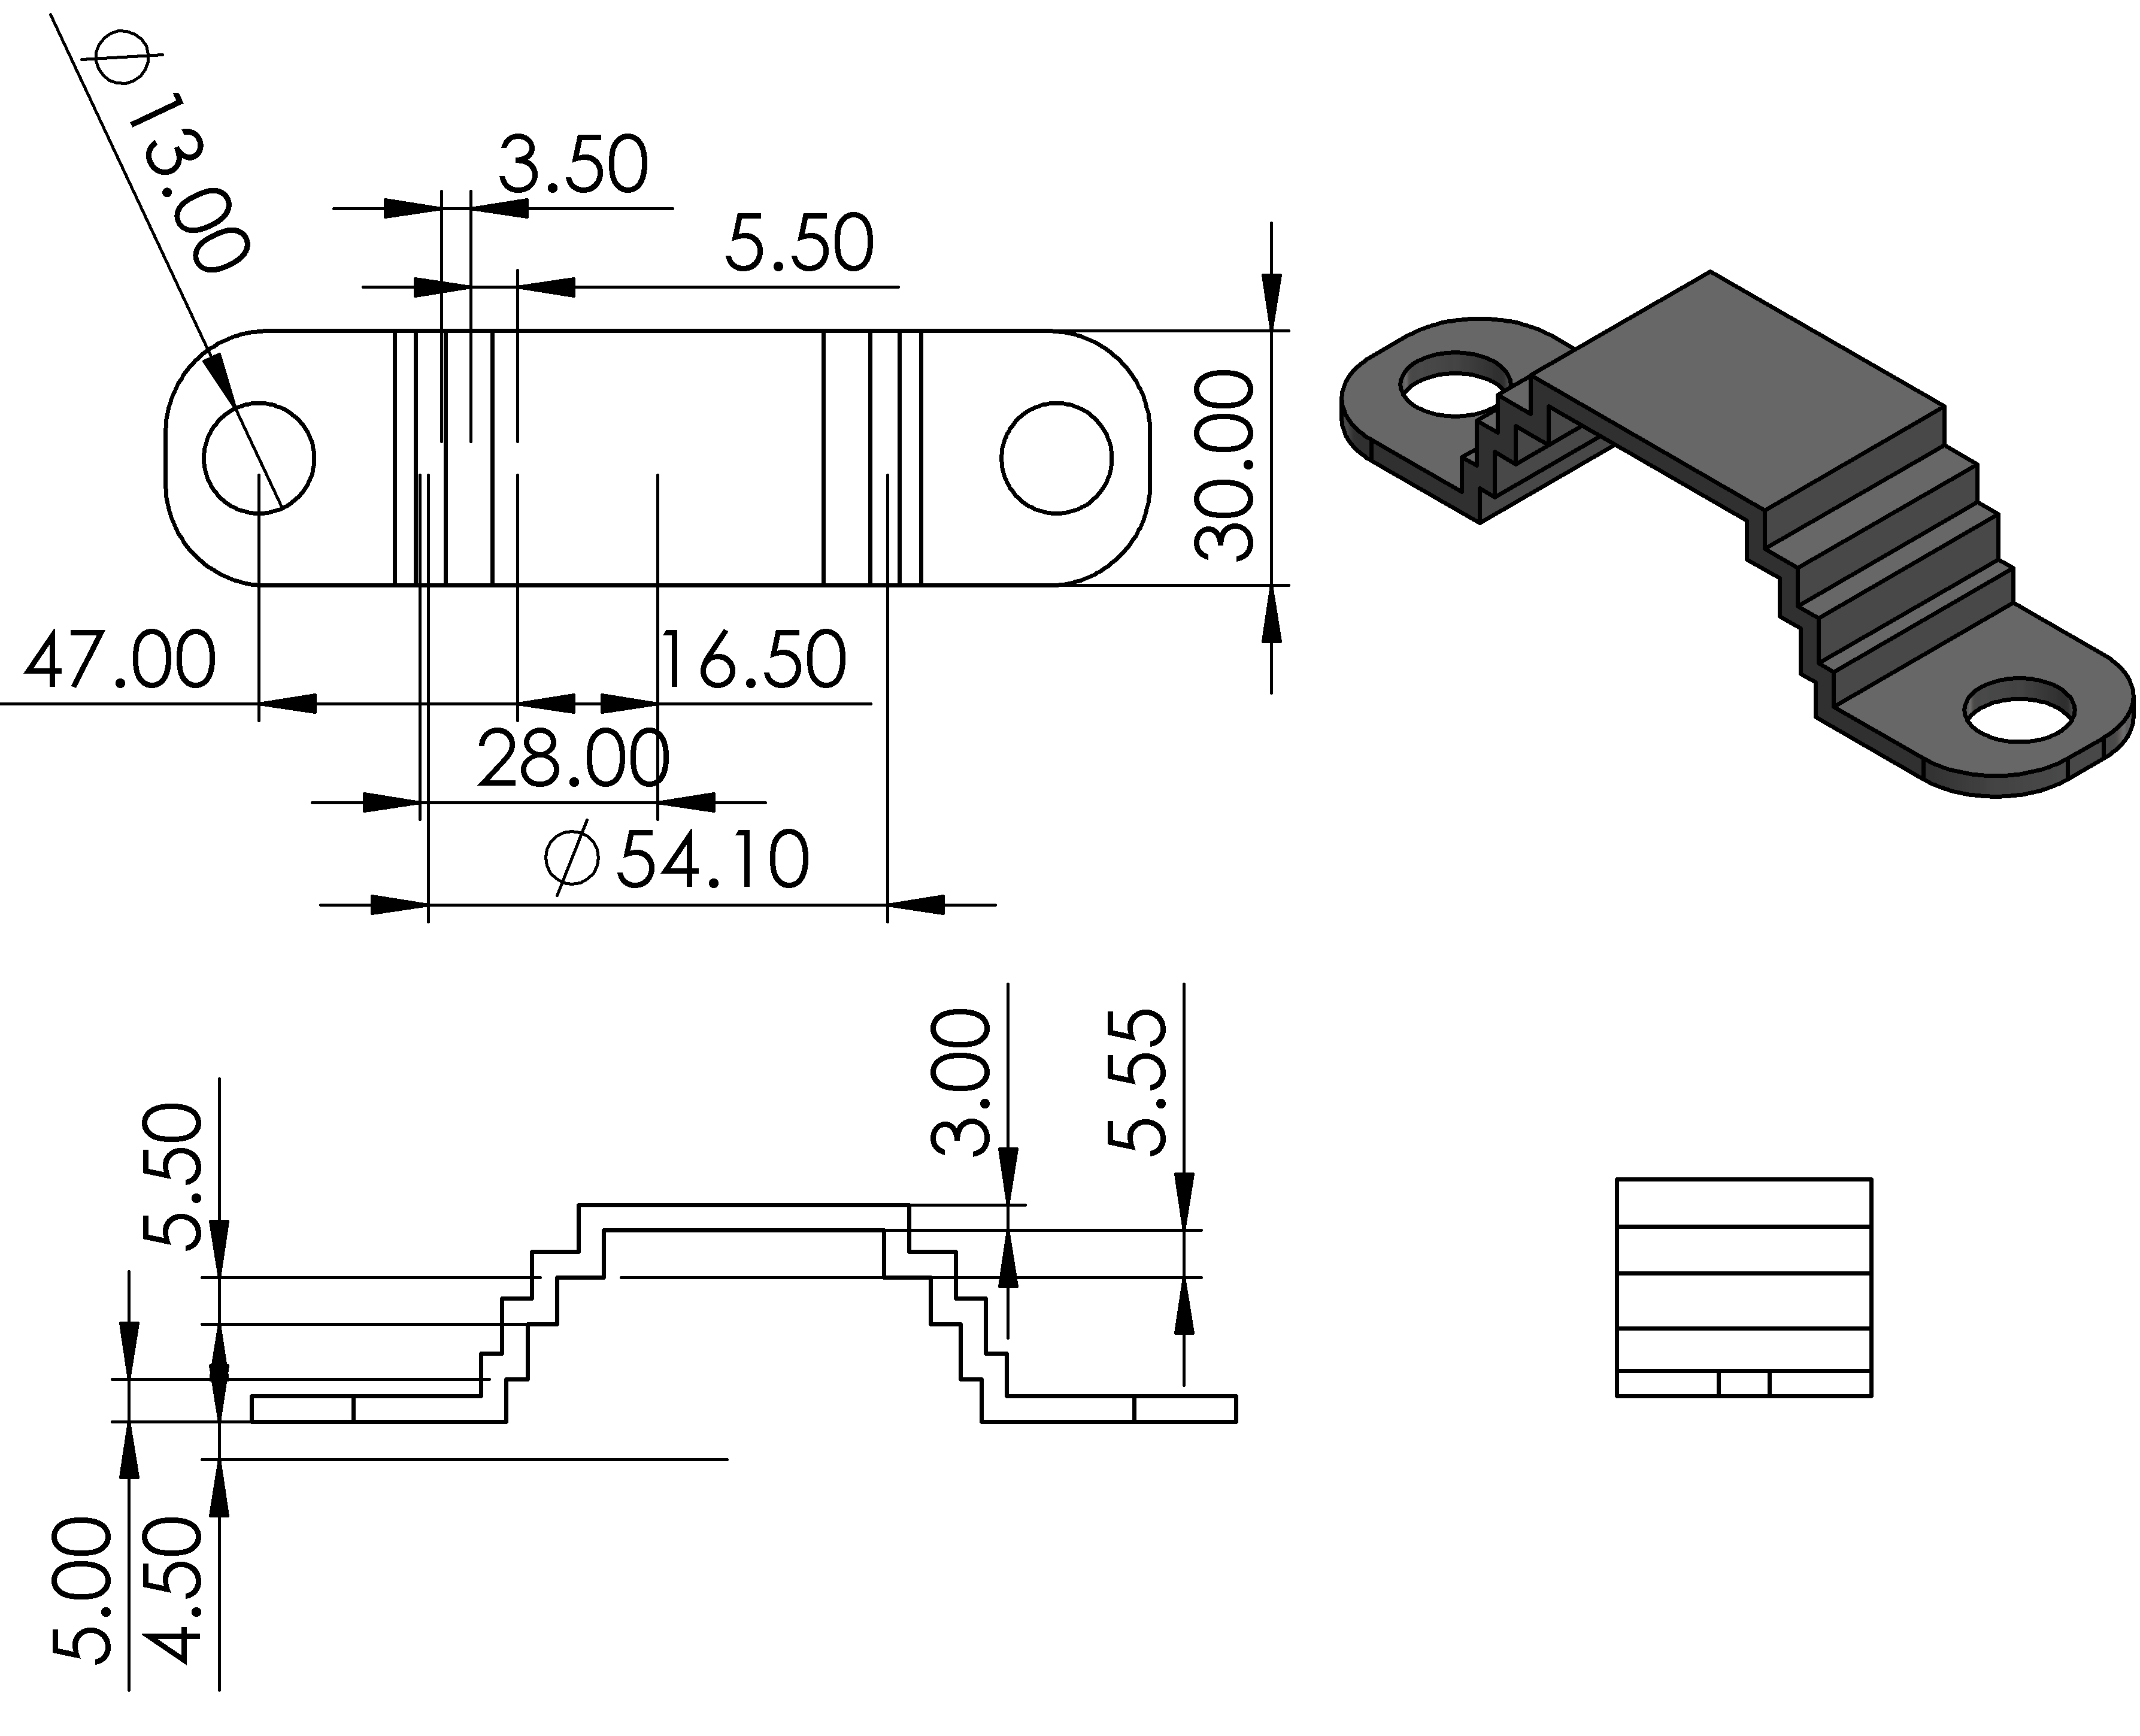
\includegraphics[height=.45\textheight]{Figures/twoRailStrapsBottom.PNG}
        \caption{Bottom strap}
        \label{fig:two_rail_serrated_straps}
    \end{figure}
      
    \par
    \item \textbf{Servo motor discharge flow control assembly}
    \par
    The assembly of parts used in the servo motor approach is as shown in Figure \ref{fig:servo_motor_discharge flow control assembly}.
     \begin{figure}[H]
         \centering
         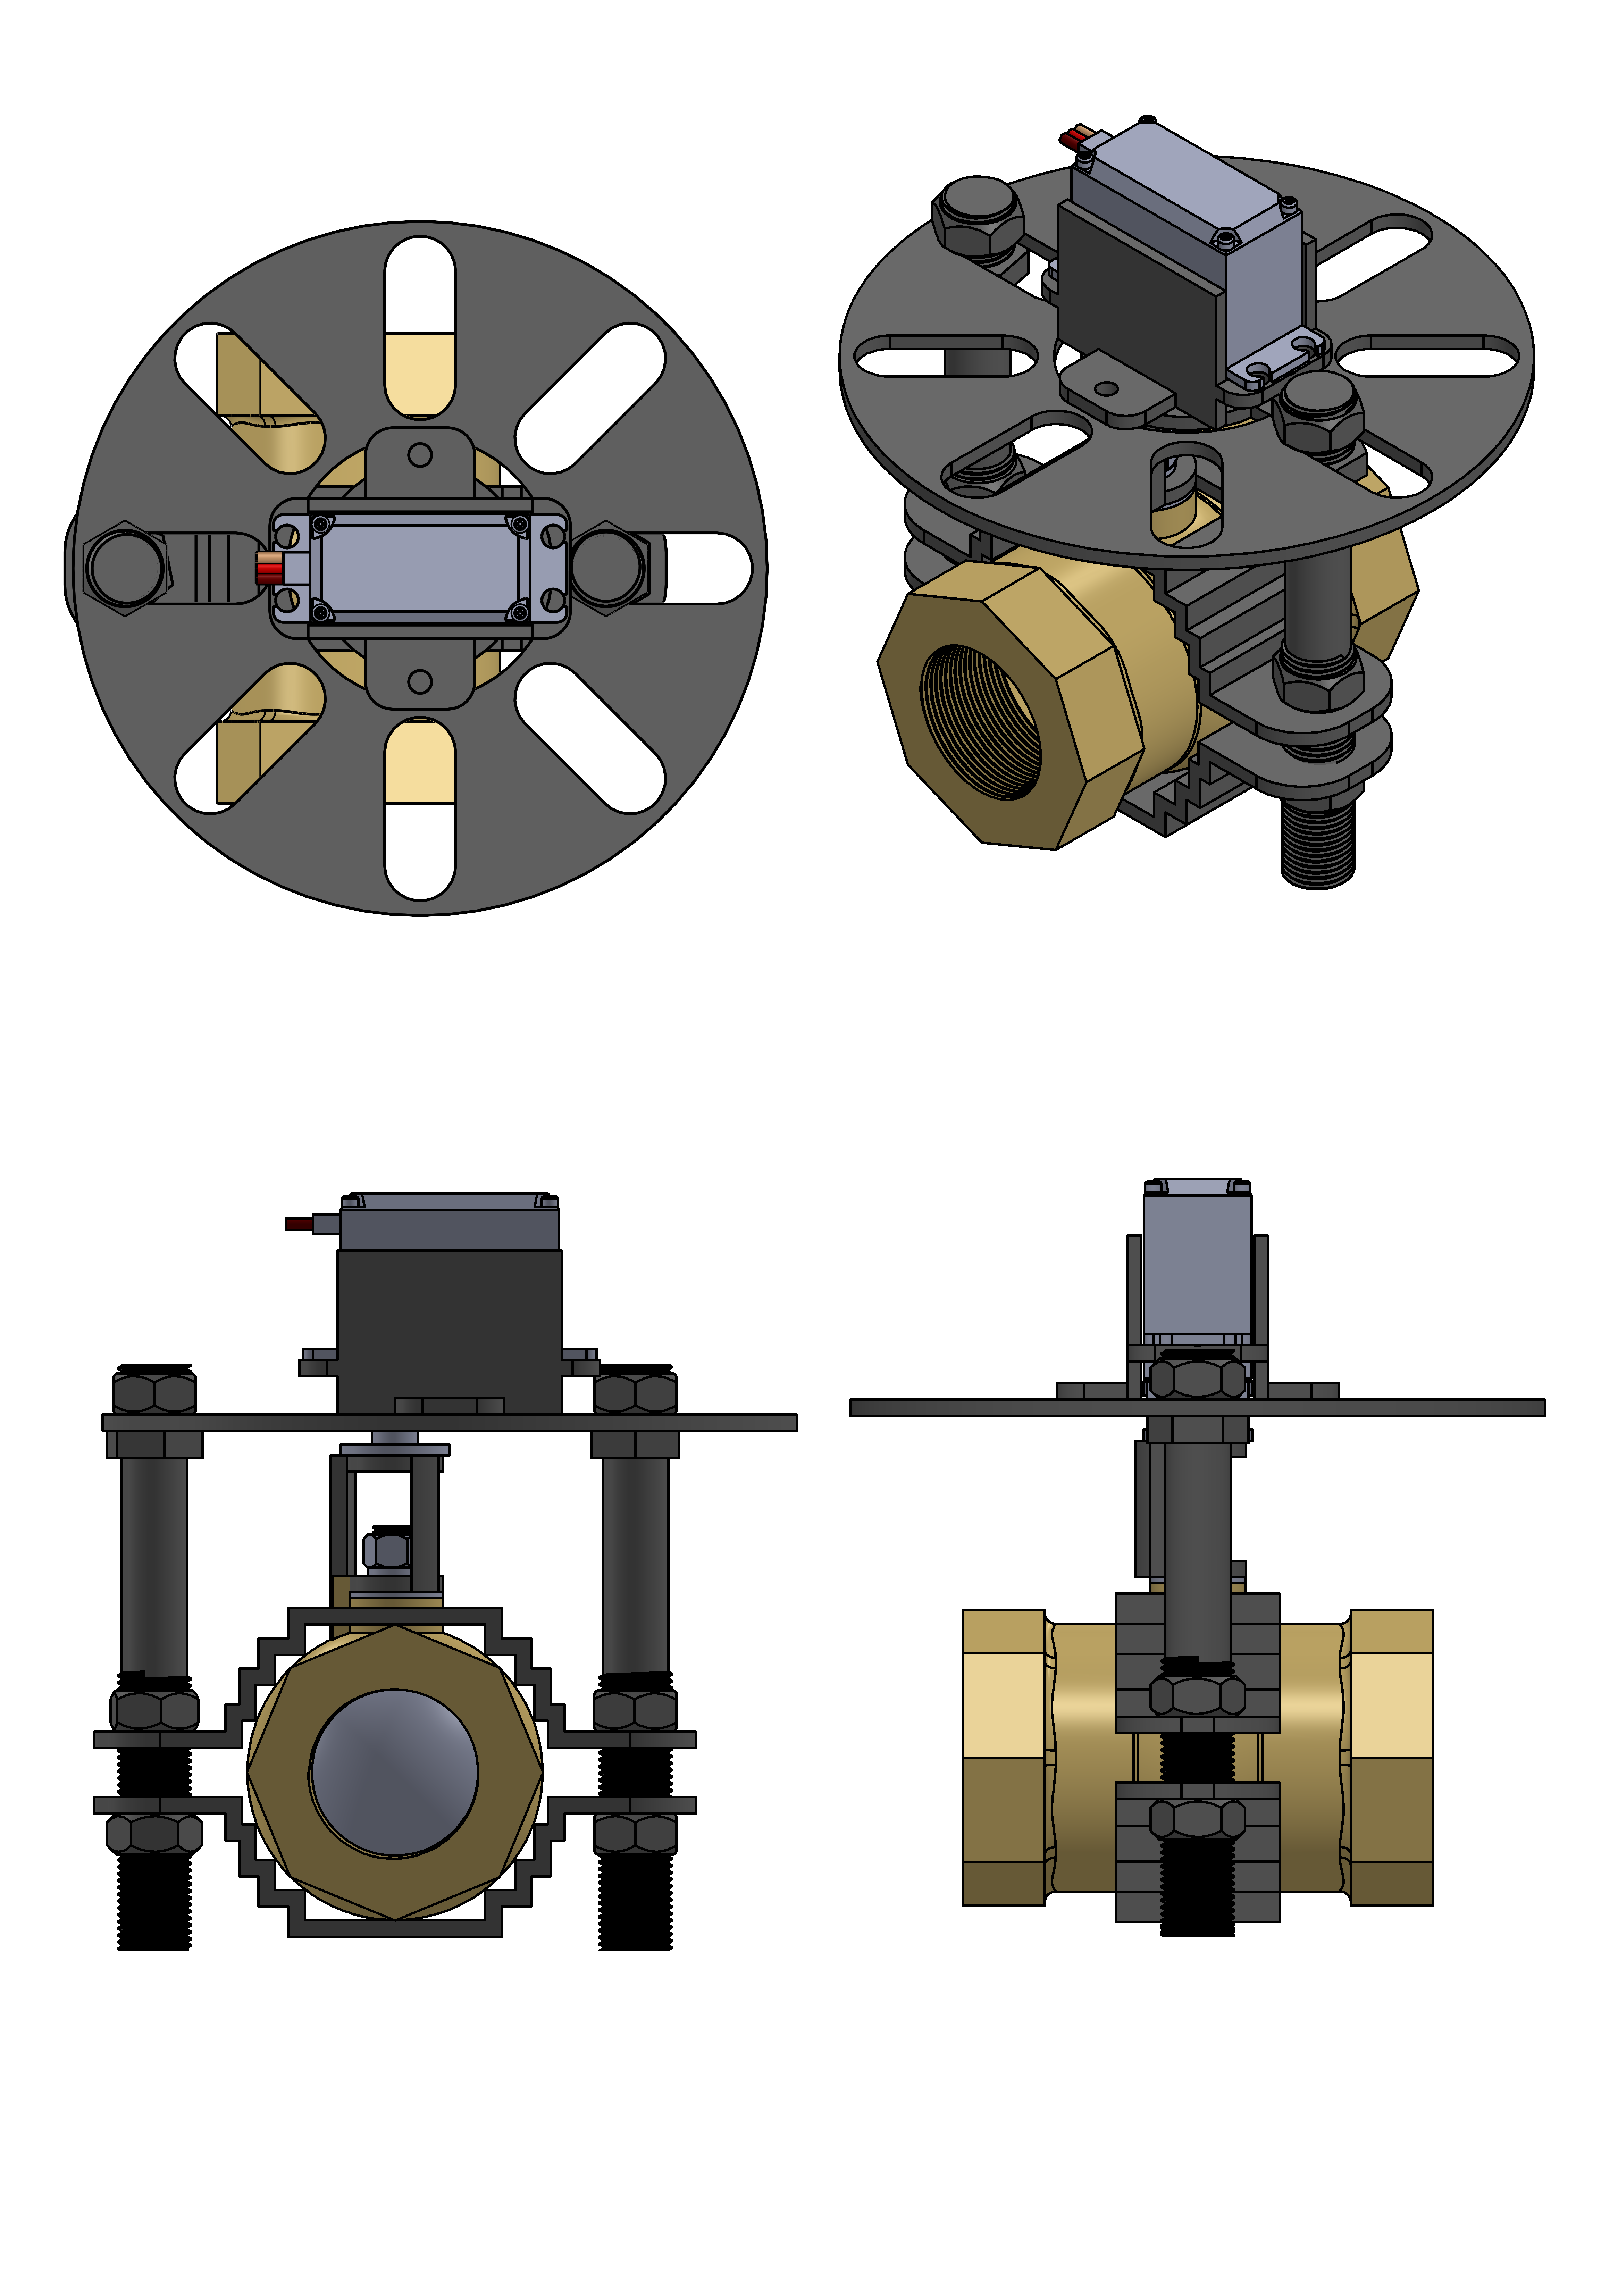
\includegraphics[height=.75\textheight]{Figures/ServoHolderBallValveAssembly.PNG}
         \caption{Servo motor discharge flow control assembly}
         \label{fig:servo_motor_discharge flow control assembly}
     \end{figure}
      
     \par
     \item \textbf{Finite element analysis of the assembly}
     \par
     PLA material was assigned to each part of the structure. The maximum load torque of the servo motor($11kg.cm$) was then applied on the mounting plate of the motor. The results of the simulation were as shown in figure \ref{fig:servo_assembly_results}. From the results, the structure still holds to the maximum torque with minimal displacement.
     \begin{figure}[H]
         \centering
         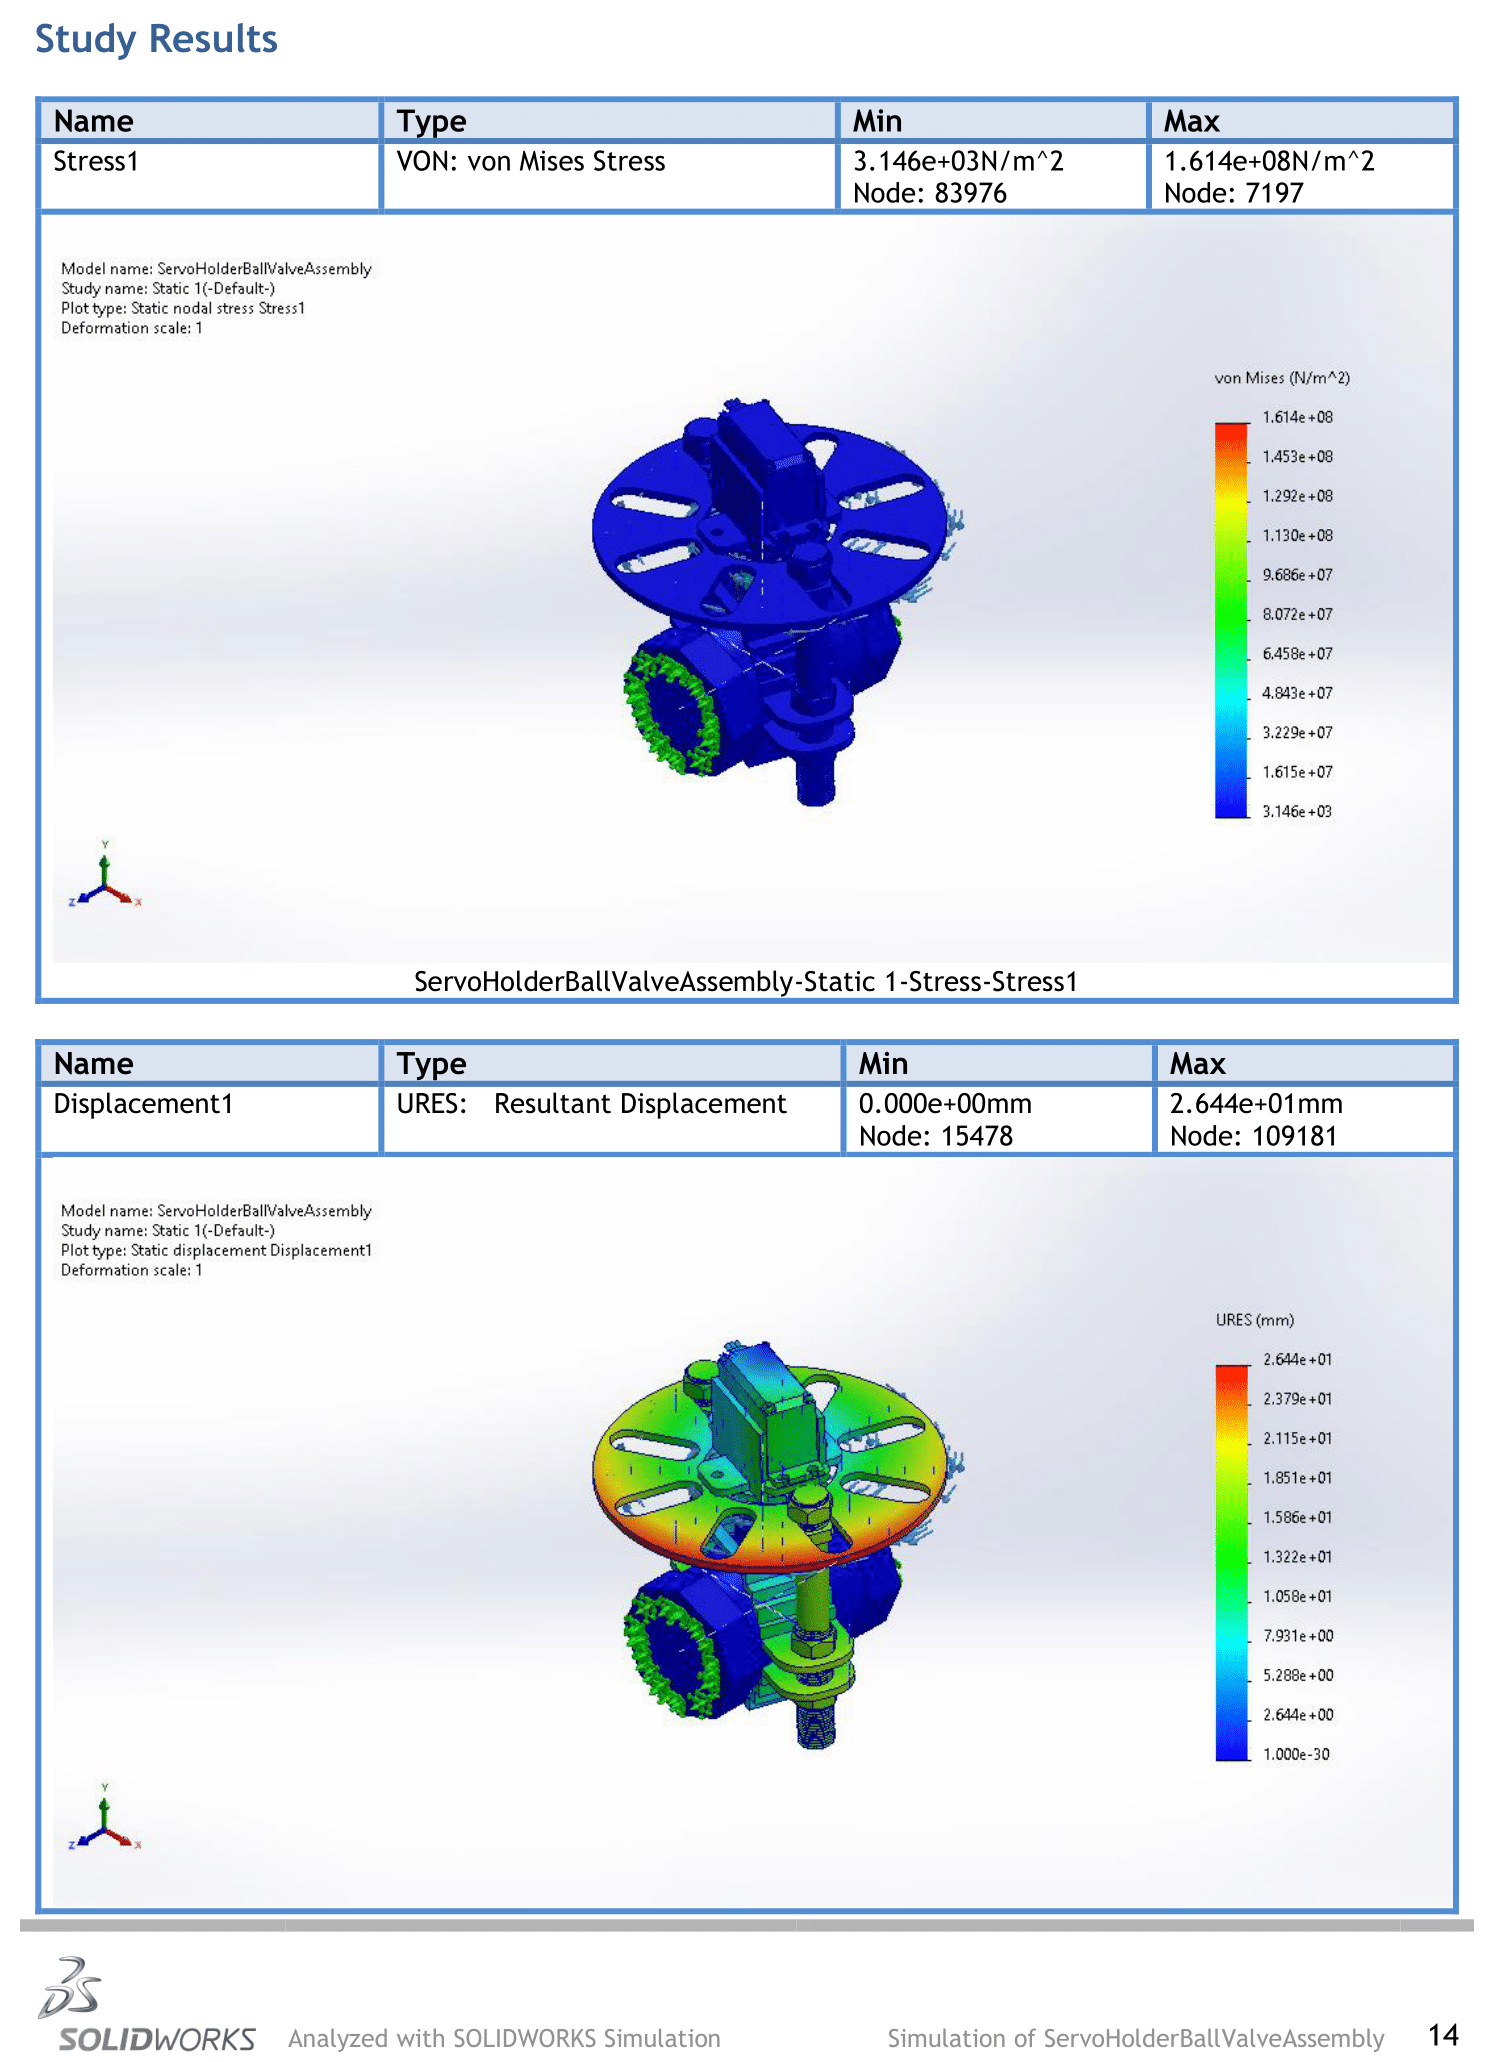
\includegraphics[width=\textwidth]{Figures/ServoHolderBallValveAssembly-Static-1-1-1.png}
         \caption{Servo Assembly simulation results}
         \label{fig:servo_assembly_results}
     \end{figure}
    \end{enumerate}
\end{enumerate}

From these two design approaches, the servo motor approach was selected.

\subsubsection{Flow diversion sub-unit}
The design of this unit was based on the following two considerations:
\begin{enumerate}
    \item A faster response time. The response time in this application is the time it takes to divert the discharge flow into the main reservoir or the discharge collection tank. 
    \item An actuator that can provide linear translation of not less than 30 mm. In fact the longer the better. This is measured from the design assembly. This ensures that the discharge is fully diverted into the collection tank or to the main reservoir. 
\end{enumerate}

Based on the above two considerations, the following two design options were feasible.
\begin{enumerate}
    \item \textbf{Piezo-electric actuator}
    \par
    Piezoelectric actuators are transducers that convert electrical energy into a mechanical displacement or stress based on a piezoelectric effect, or vice versa. They are widely used as a high-precision positioning mechanism since they can control a small mechanical displacement at high speed, with the advantages of large generated force, stable displacement, and ease of use\cite{gao2020piezoelectric}. 
    \par
    Among the many advanced piezoelectric actuators on the market, a Xeryon Precision XLA-Series 3 piezo actuator shown in Figure \ref{fig:piezo_actuator} was selected since it satisfied all the design requirements required for this subunit.
    \begin{figure}[H]
        \centering
        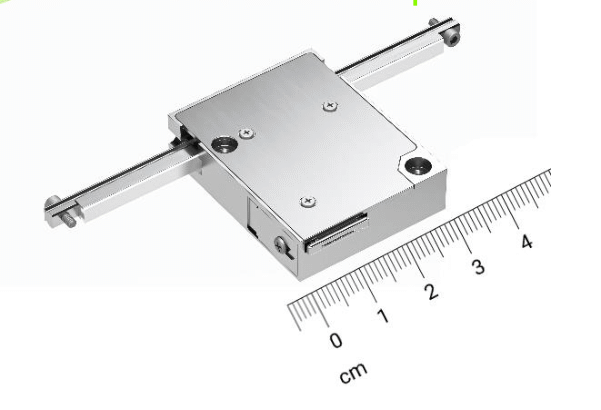
\includegraphics{Figures/Xeryon-XLA-3-1.png}
        \caption[Xeryon-XLA Series 3 piezo actuator]{Xeryon-XLA Series 3 piezo actuator \cite{xla3}}
        \label{fig:piezo_actuator}
    \end{figure}
    Its technical specifications are as shown in table \ref{tab:XLA_stuff}.
    \begin{table}[H]
    \centering
    \begin{tabular}{|l|l|}
    \hline
    \textbf{Property} & \textbf{Value} \\ \hline
    Stroke Length & 45mm \\ \hline
    Resolution & 312nm \\ \hline
    Operating voltage & 20-48V \\ \hline
    Control & Closed loop control with an external XD-A controller \\ \hline
    Temperature & -30  to 70 \\ \hline
    Holding\& Driving  force & 3N \\ \hline
    Speed range & 2mm / s to 400mm / s \\ \hline
    \end{tabular}
    \caption[XLA series 3 piezo actuator specifications]{XLA series 3 piezo actuator specifications \cite{xla3}}
    \label{tab:XLA_stuff}
    \end{table}
    
    
    From the technical specifications in the table, it is evident that this actuator could be the best choice for this application. However, it requires an external proprietary controller for closed-loop control. Xeryon company products are also not available in public stores such as Amazon or Aliexpress.
    
    \item \textbf{Electromagnetic Actuator}
    \par
    Electromagnetic actuators work on the principle of electromagnetism. Electrical energy is converted to a linear translational mechanical motion and vice versa. The electric current serves as the actuator quantity in electromagnetic actuators.
    \par
    Based on the design considerations, a P16-S micro linear actuator shown in figure \ref{fig:p16_s_linear_actuator}  was selected for this application.
    \begin{figure}[H]
        \centering
        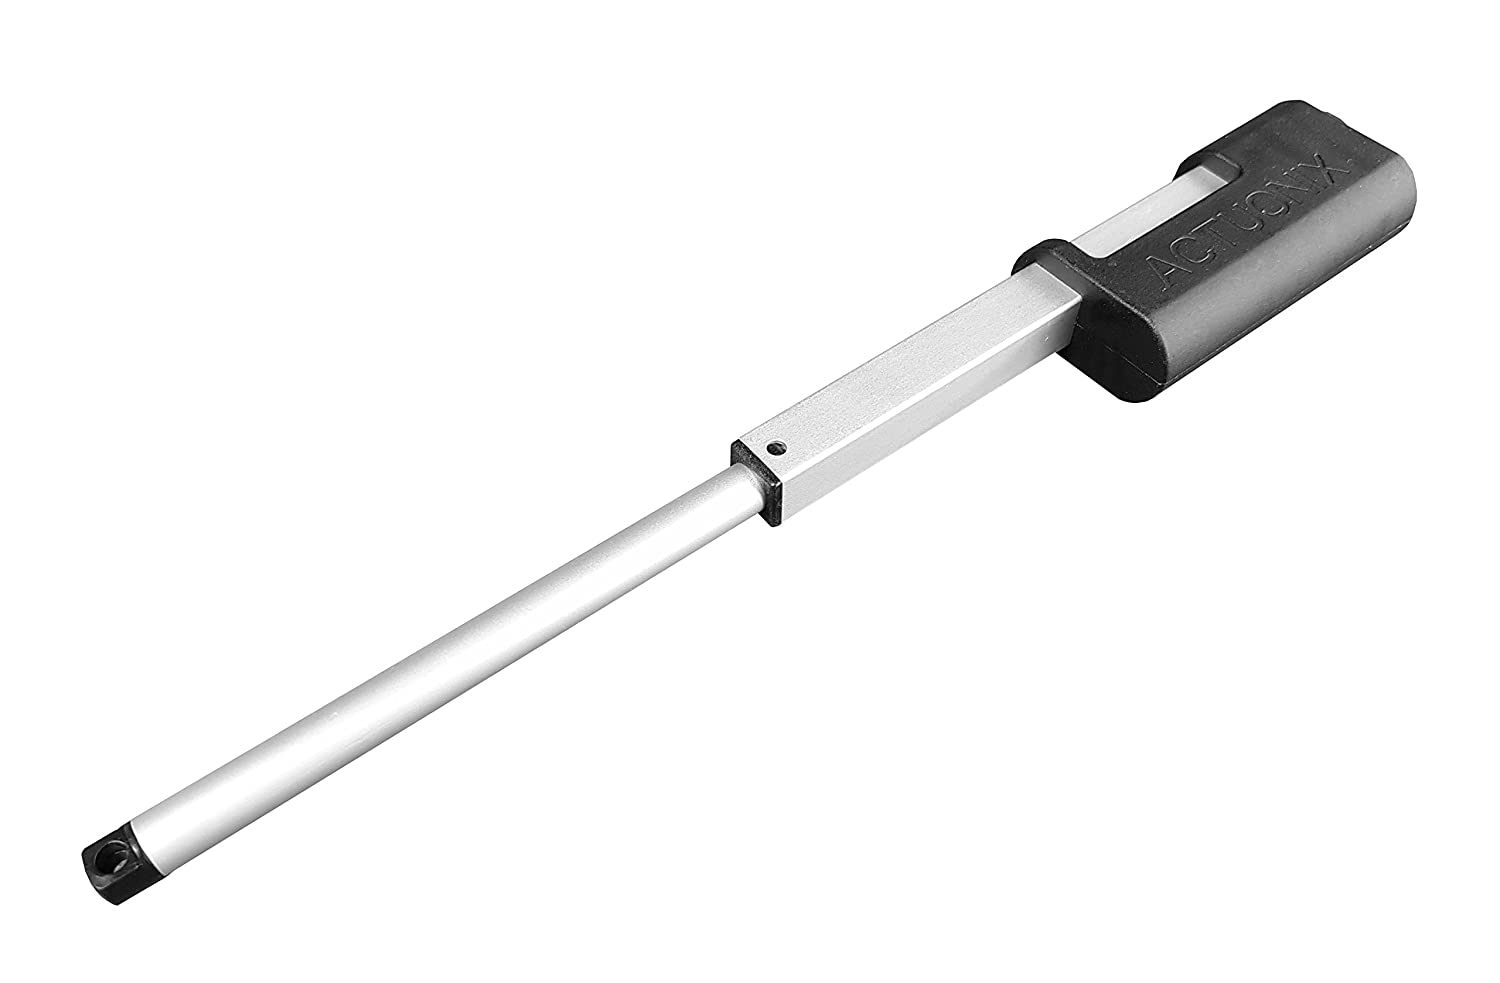
\includegraphics[width=.25\textwidth, height=.25\textheight]{Figures/P16S.jpg}
        \caption[P16S linear actuator]{P16S linear actuator \cite{p16_s}}
        \label{fig:p16_s_linear_actuator}
    \end{figure}
    Its technical specifications are shown in table \ref{tab:p16_s}.
    \begin{table}[H]
    \centering
    \begin{tabular}{|l|l|}
    \hline
    \textbf{Property} & \textbf{Value} \\ \hline
    Operating voltage & 12V DC \\ \hline
    Stroke length & 100mm \\ \hline
    Stroke speed & 150mm/s \\ \hline
    Maximum load & 6.4N \\ \hline
    \end{tabular}
    \caption[P16-S Micro-linear actuator technical specifications]{P16-S Micro-linear actuator technical specifications \cite{p16_s}}
    \label{tab:p16_s}
    \end{table}
    From the technical specifications in the table, it is also evident that this actuator satisfies optimumly the requirements required for this application. Unlike the piezo actuator, this device is available for less than \$ 35 in e-Commerce stores such as Amazon or AliExpress.
\end{enumerate}

Based on the above descriptions, the P16-S micro-linear actuator was selected for this application mainly because of its availability.
\par
In order to hold this actuator in position the following designs were made:
\begin{enumerate}
    \item \textbf{Electromagnetic Actuator holder}
    \par
    This unit supports the actuator on the ball valve. It is required that this unit will withstand the weight of both the actuator and the diverter. It design is as shown in figure \ref{fig:electromagnetic_actuator}.
    \begin{figure}[H]
        \centering
        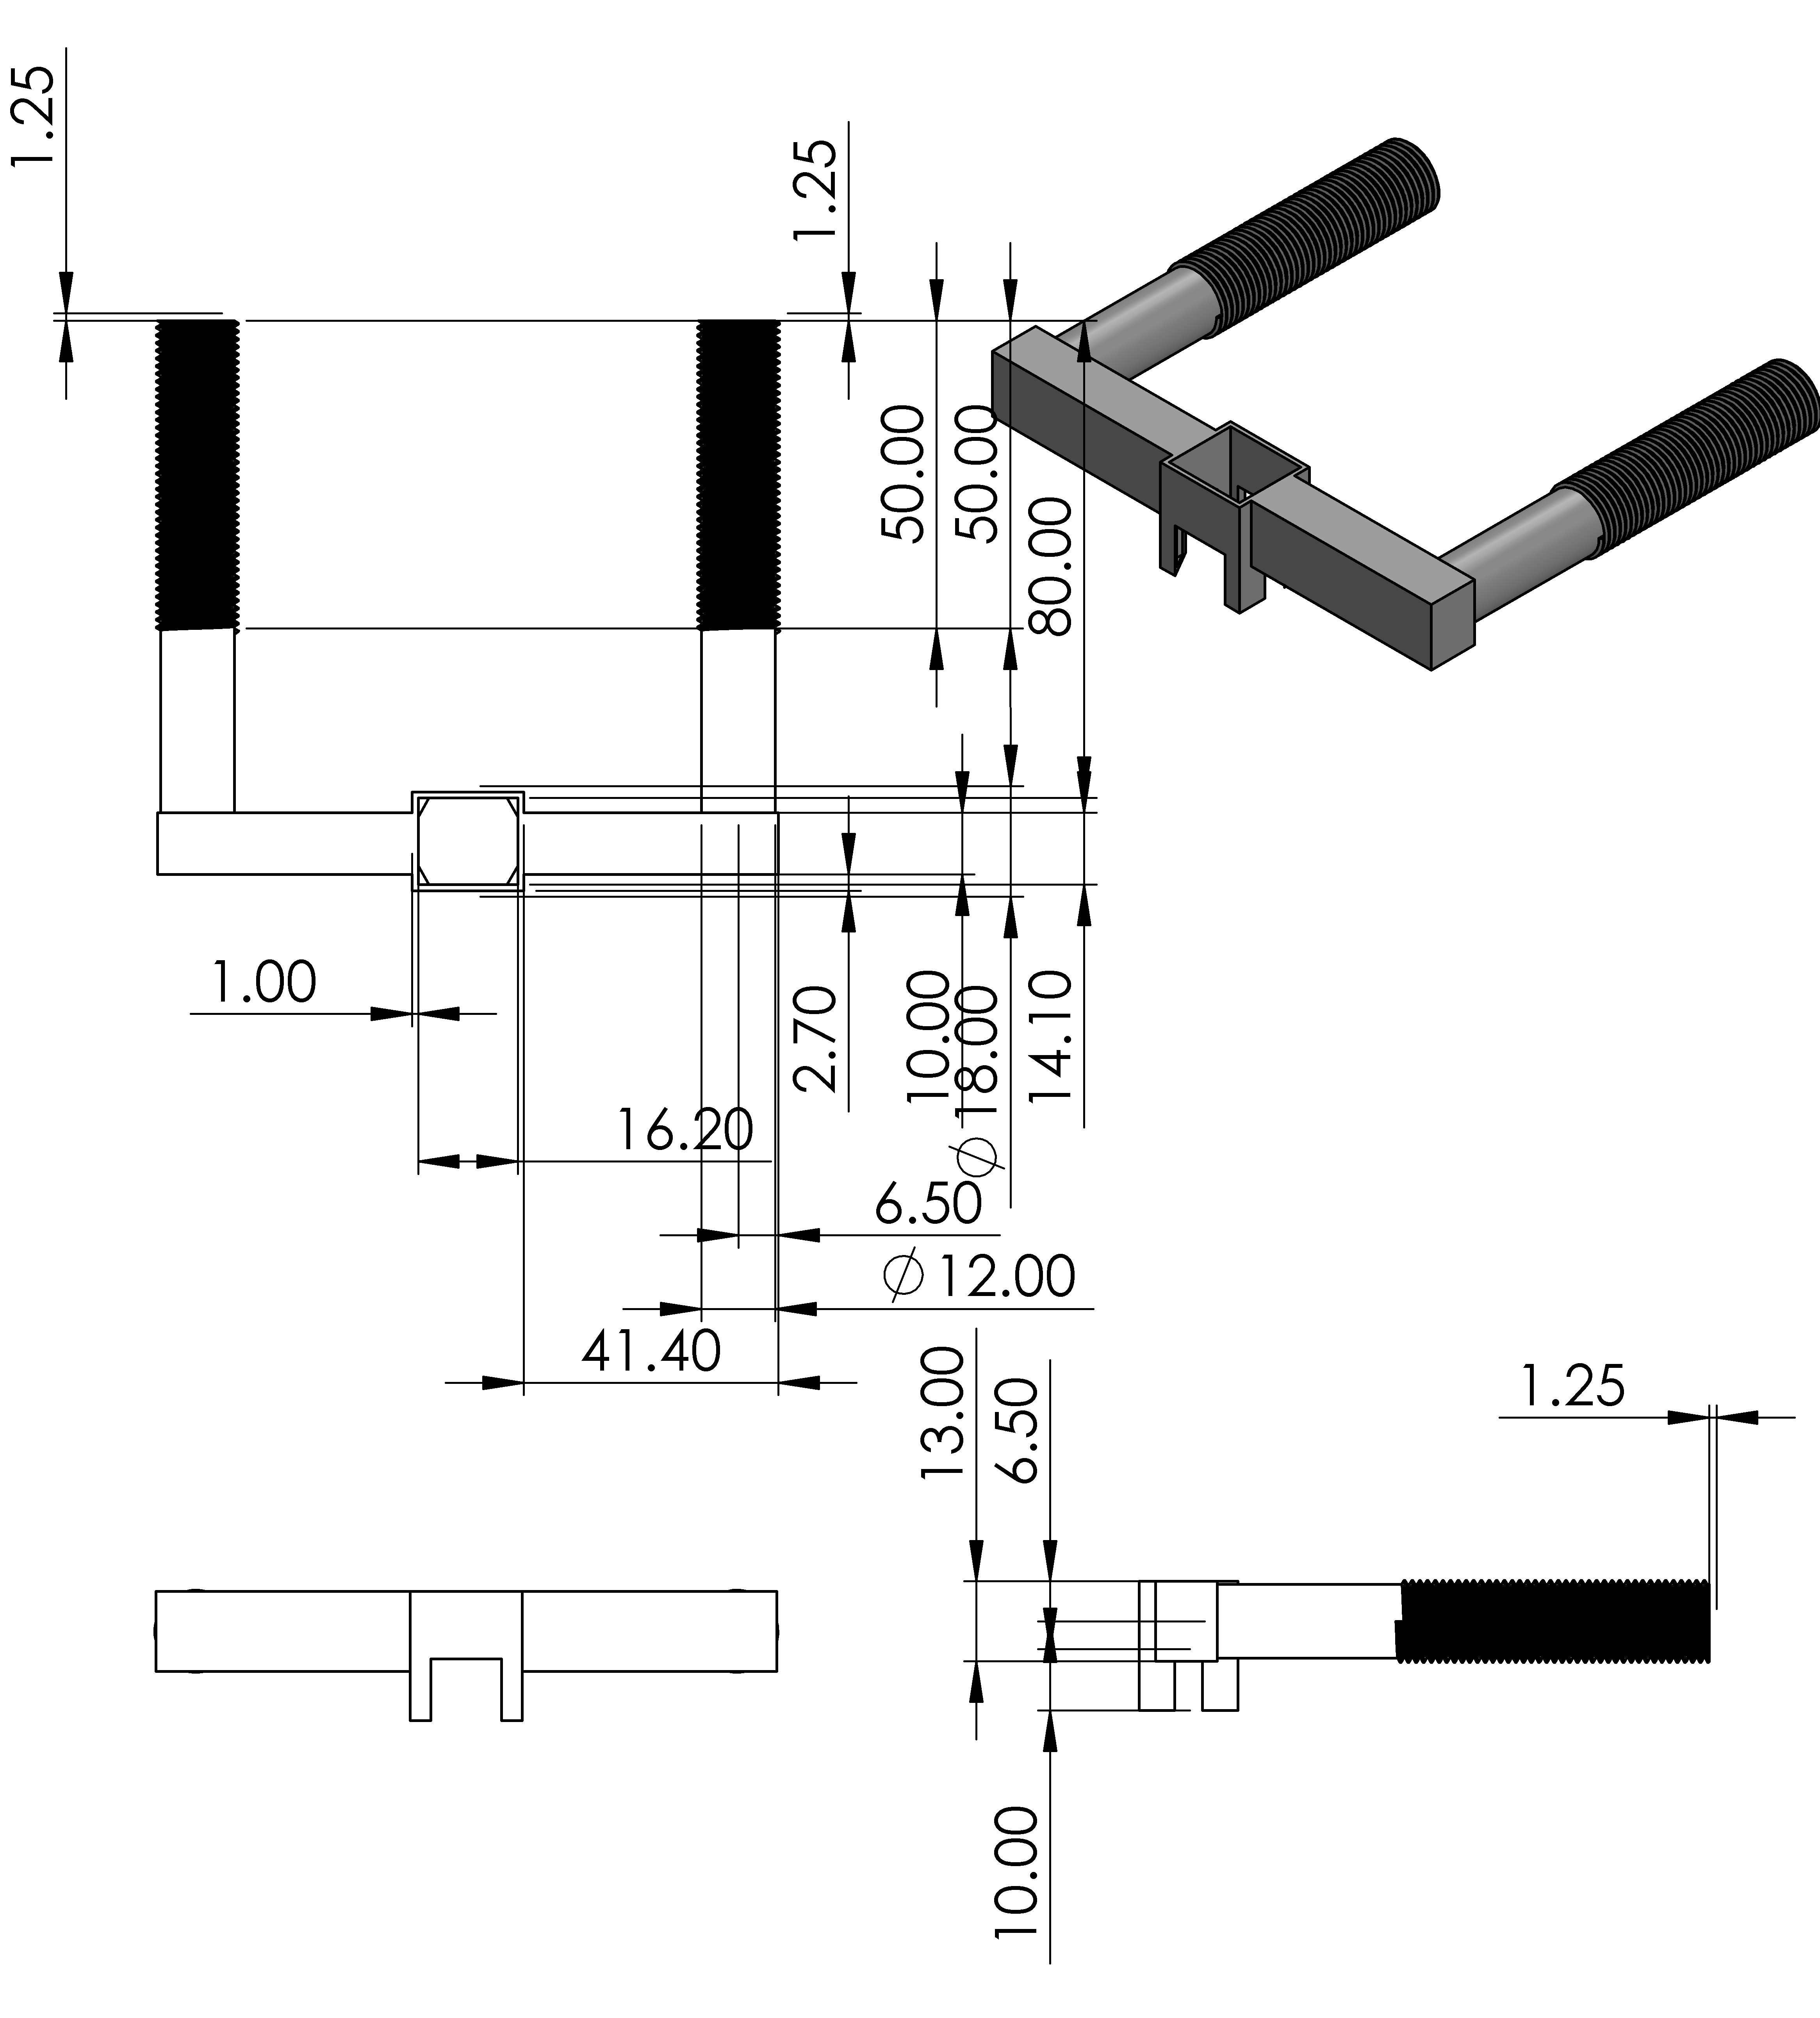
\includegraphics[height=.65\textheight]{Figures/ElectromagnetHolder.PNG}
        \caption{Electromagnetic actuator holder}
        \label{fig:electromagnetic_actuator}
    \end{figure}
    The dimensions of this holder design were determined from the dimensions of the P16-S linear actuator plus a clearance of 0.5mm.
    
    \item \textbf{Diversion Flap}
    \par
    In order to divert the flow, a channel-like flap is to be used. The design of the flap is as shown in figure \ref{fig:diversion_flap}. 
    \begin{figure}[H]
        \centering
        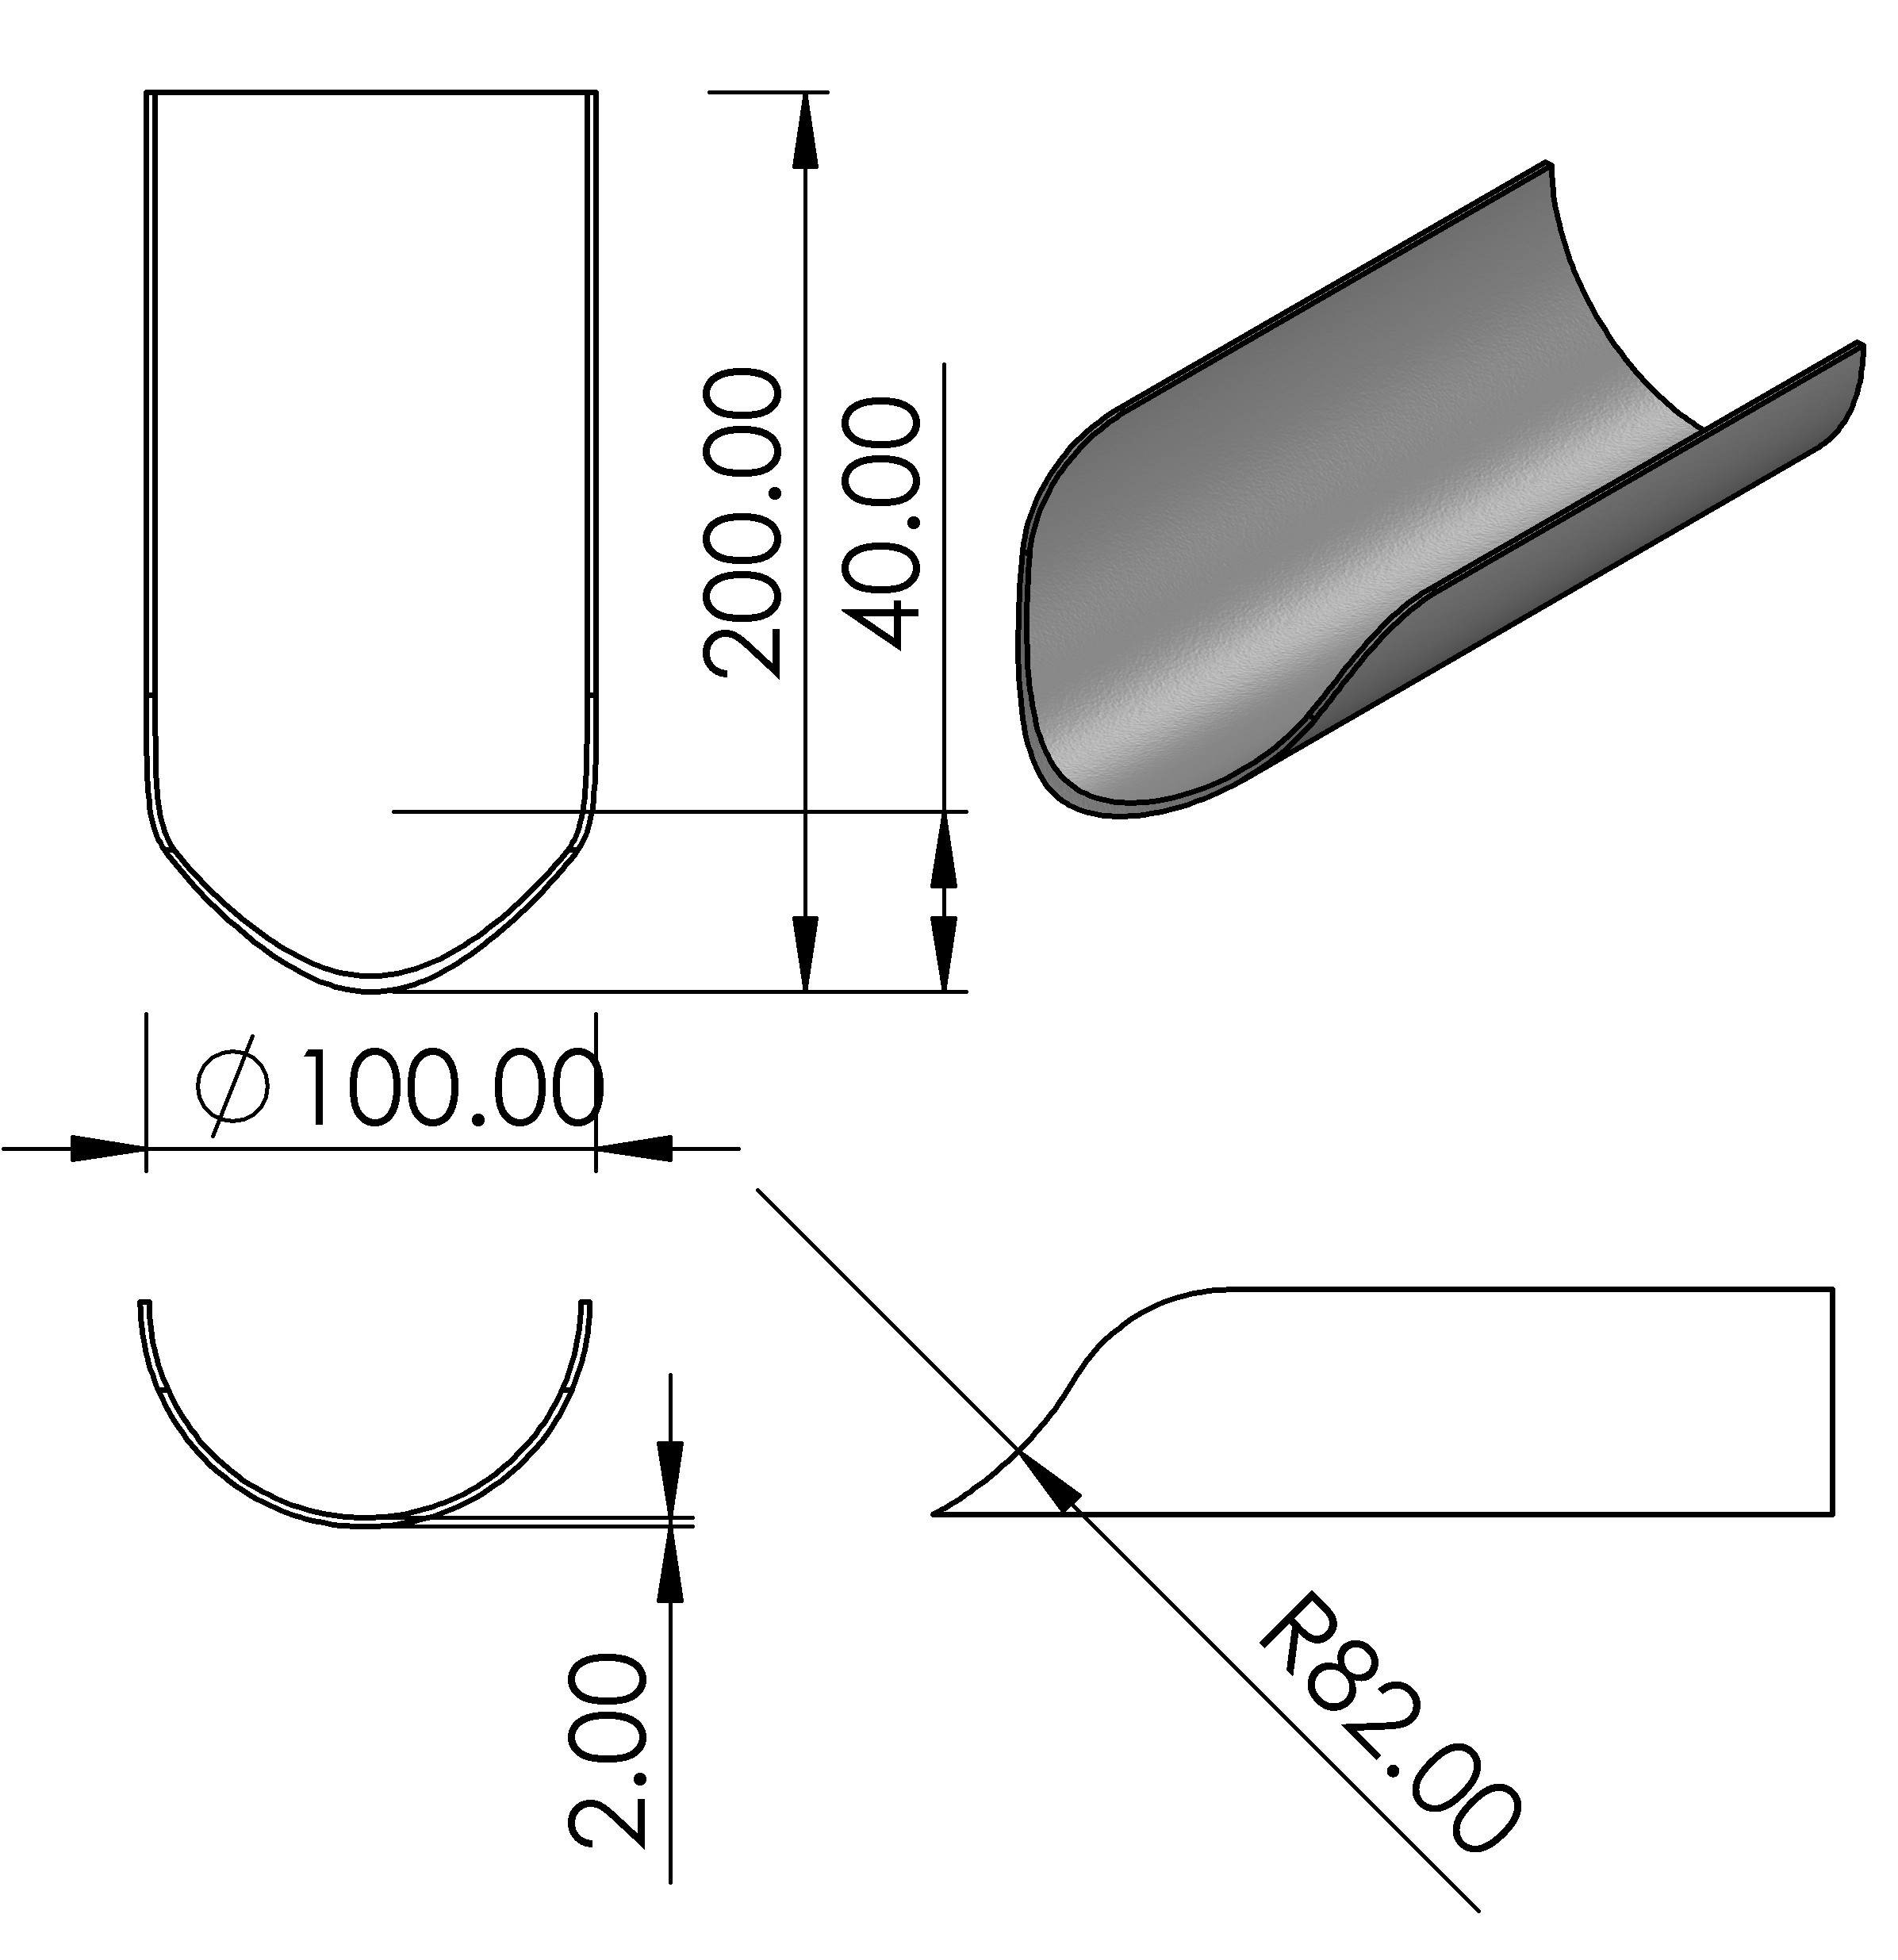
\includegraphics{Figures/flap2.PNG}
        \caption{Diversion flap}
        \label{fig:diversion_flap}
    \end{figure}
    The design was such that it can tap the whole stream from the $1\frac{3}{4} inch$ main discharge pipe on the main machine. Its 150mm length is determined by the length of the gap between the discharge pipe and the collection unit.
    \item \textbf{Flap support frame}
    \par
    This structure supports the diversion flap in place below the discharge pipe. This design was necessary since there is no convenient mounting point on the main machine that can allow the flap to be mounted without making changes to the main machine. It design is as shown in figure \ref{fig:flap_support_frame}.
    \begin{figure}[H]
        \centering
        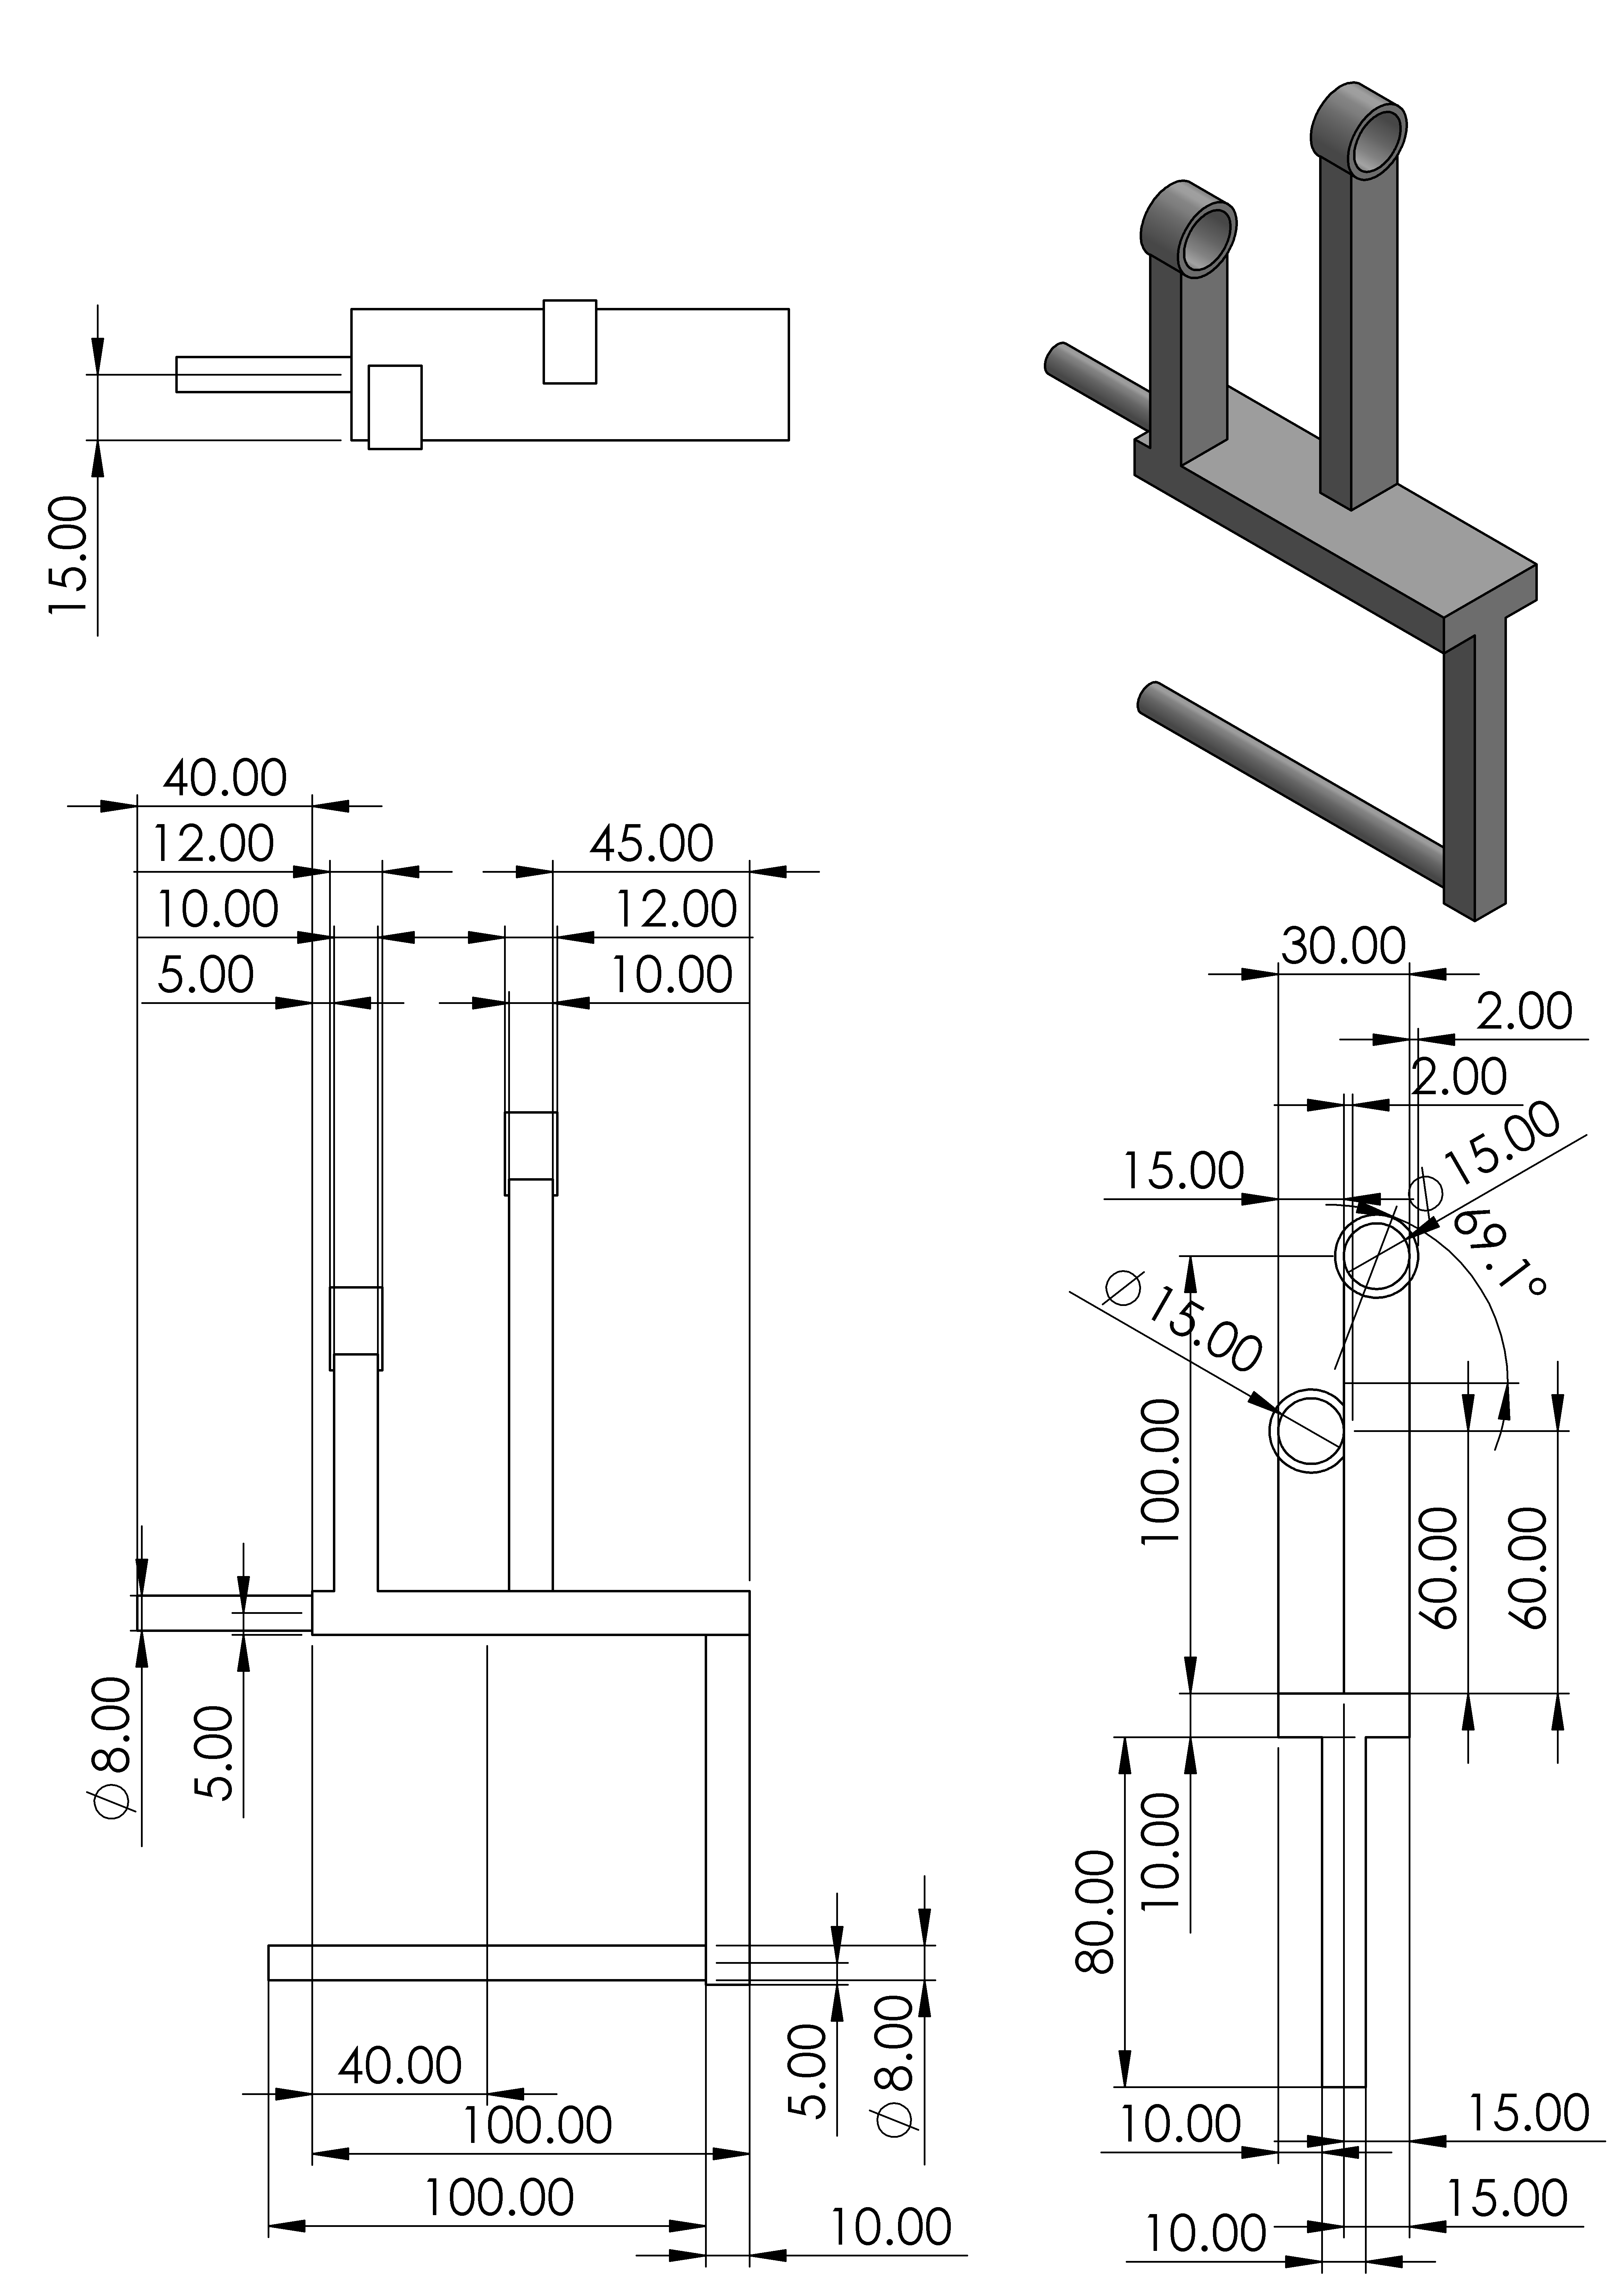
\includegraphics[height=.7\textheight]{Figures/DiversionSupport.PNG}
        \caption{Flap support frame}
        \label{fig:flap_support_frame}
    \end{figure}
    This frame also provides an extension for supporting the kinematic chain that flexes the flap. 
    \item \textbf{Kinematic Link}
    \par
    To amplify the 100mm translation in order to flex the flap enough, a four-bar kinematic mechanism is used. The lengths of the links and the orientation of the four bars are determined by assuming a translation of 100mm at the output.
    \par
    Using the MechDesigner software, the kinematic chain was designed to provide the required motion for the flap. The CAM data from its simulation was exported automatically to a SolidWorks model of the fixed point of the part.
    \begin{enumerate}
        \item \textbf{Crank}
        \par
        The input translation from the linear electromagnetic actuator. The design of this link is as shown in figure \ref{fig:crank}.
        \begin{figure}[H]
            \centering
            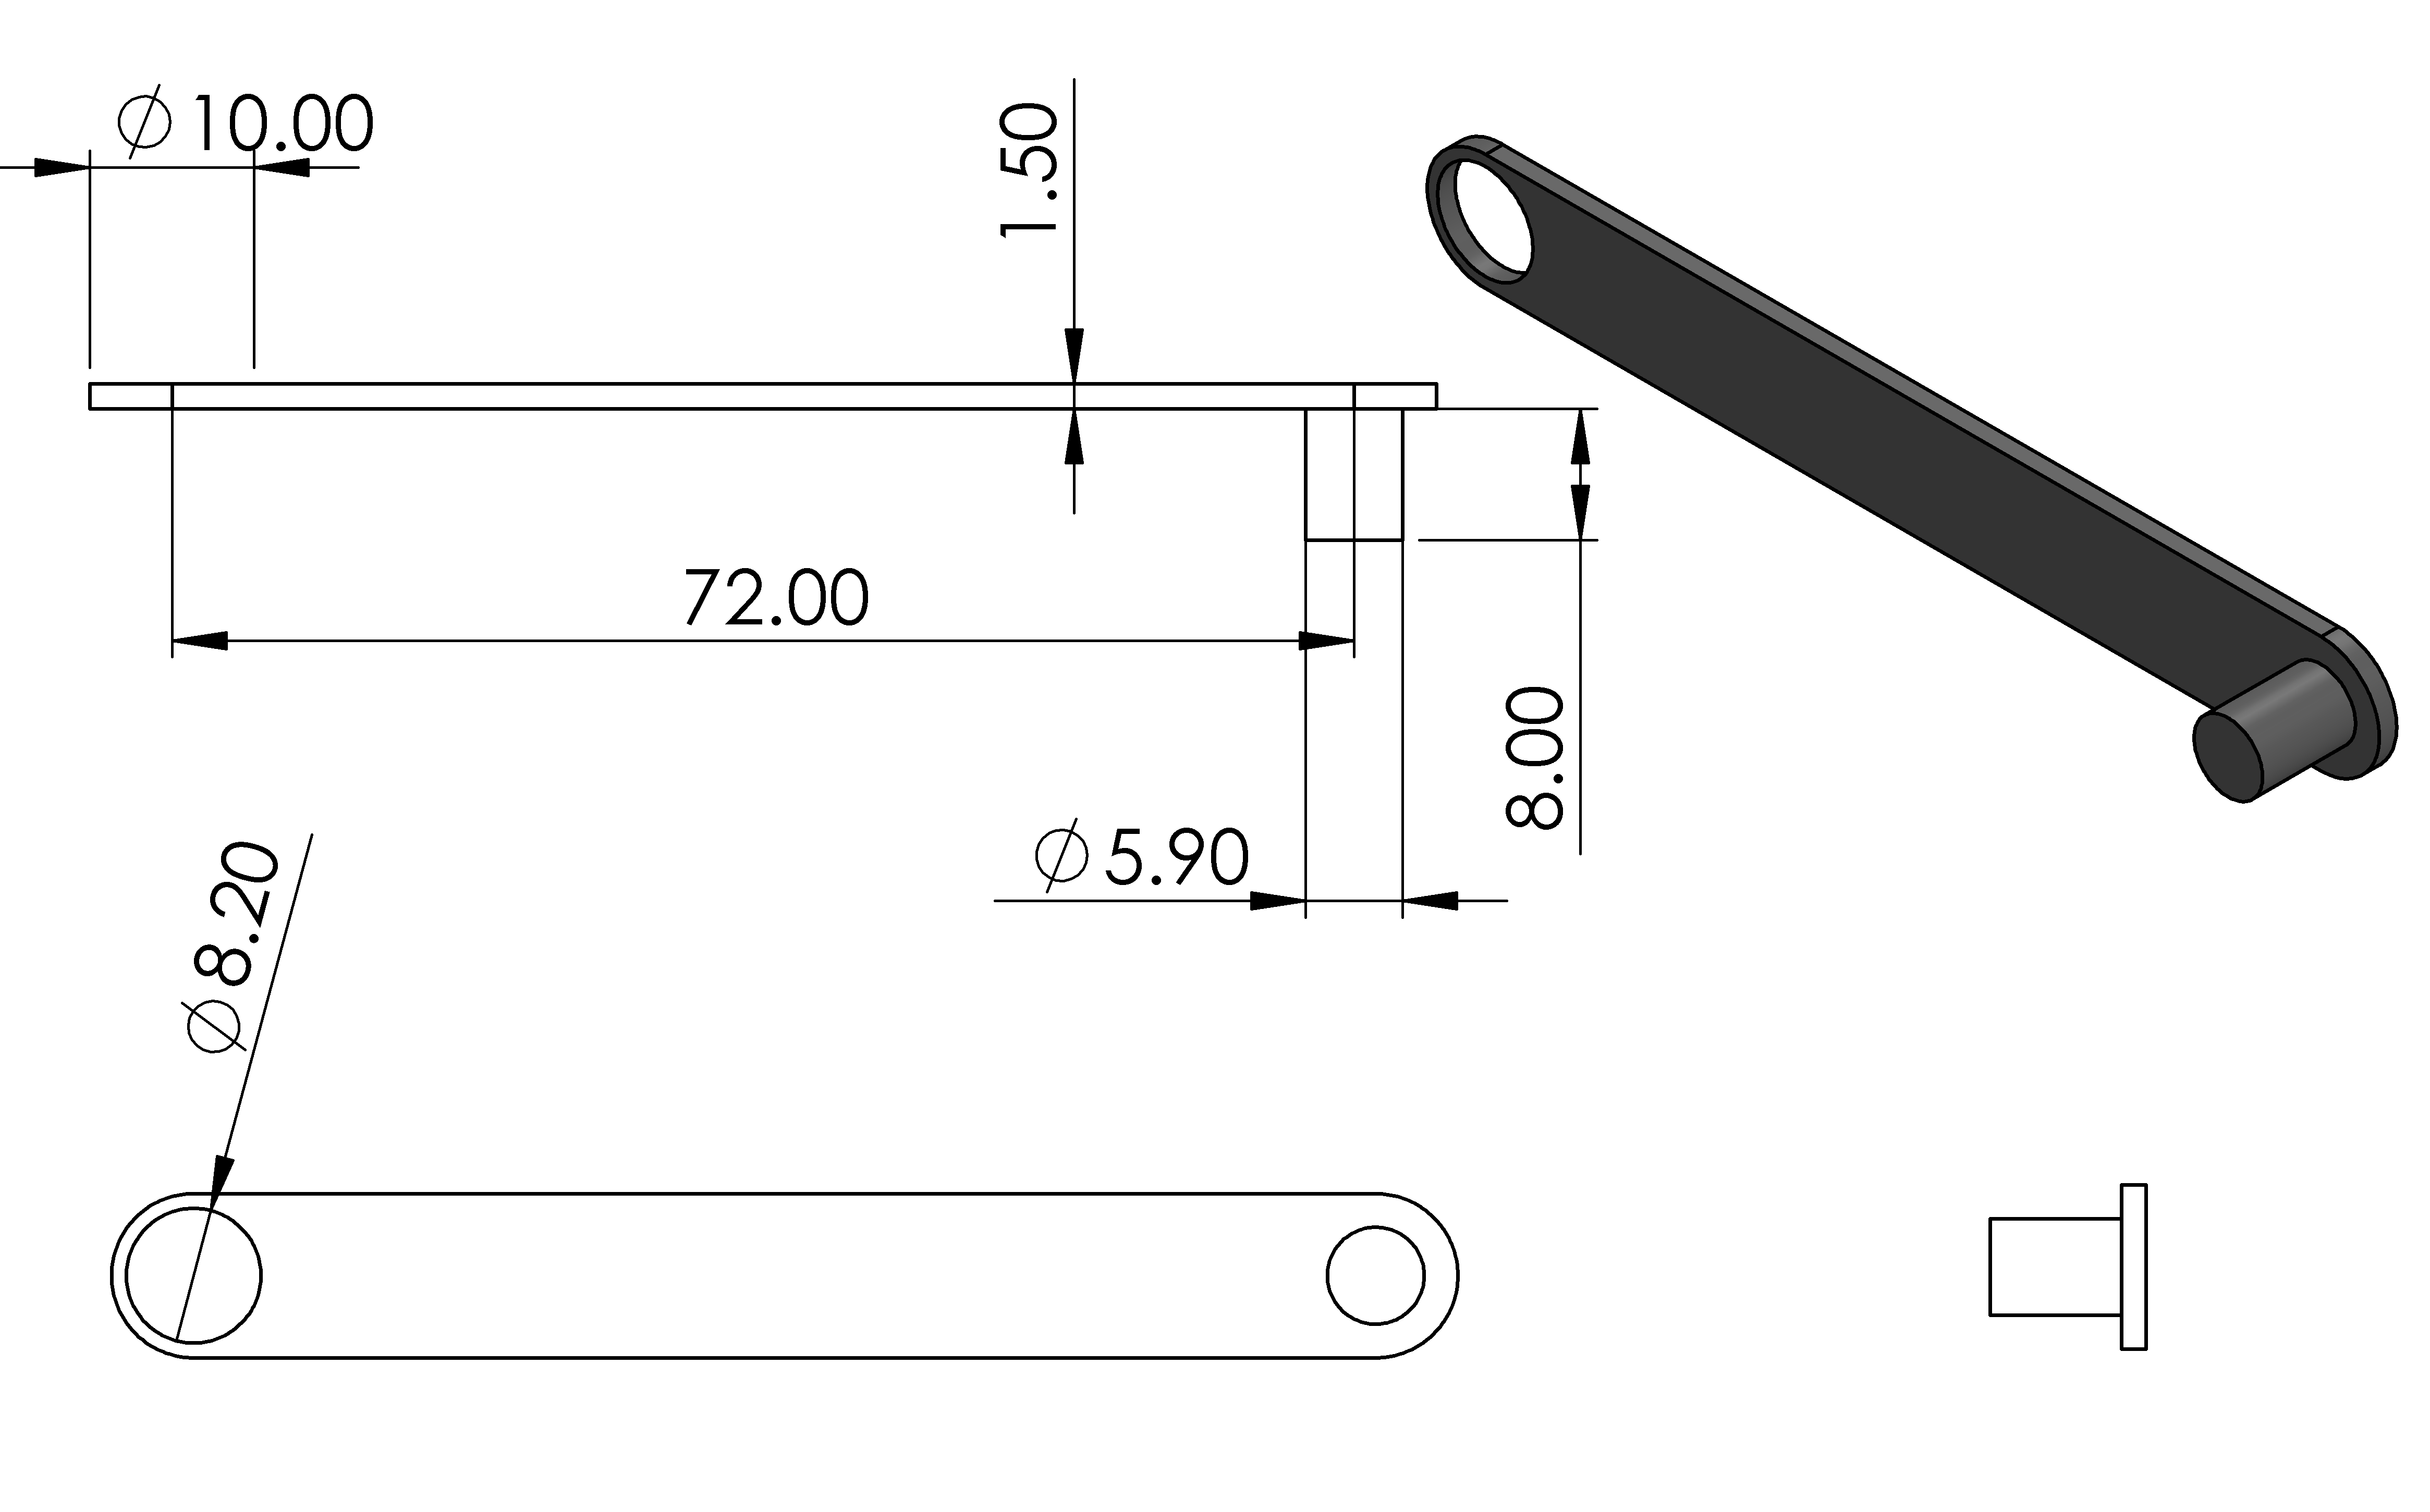
\includegraphics{Figures/KLink3.PNG}
            \caption{Crank}
            \label{fig:crank}
        \end{figure}
        The connection between this link, the end of the actuators and the couple is a series of joints. The translation is in two axes: X and Y axes.
        \item \textbf{Coupler}
        \par
        This link transfers the motion to the output link: the rocker. Its design is shown in Figure \ref{fig:coupler}.
        \begin{figure}[H]
            \centering
            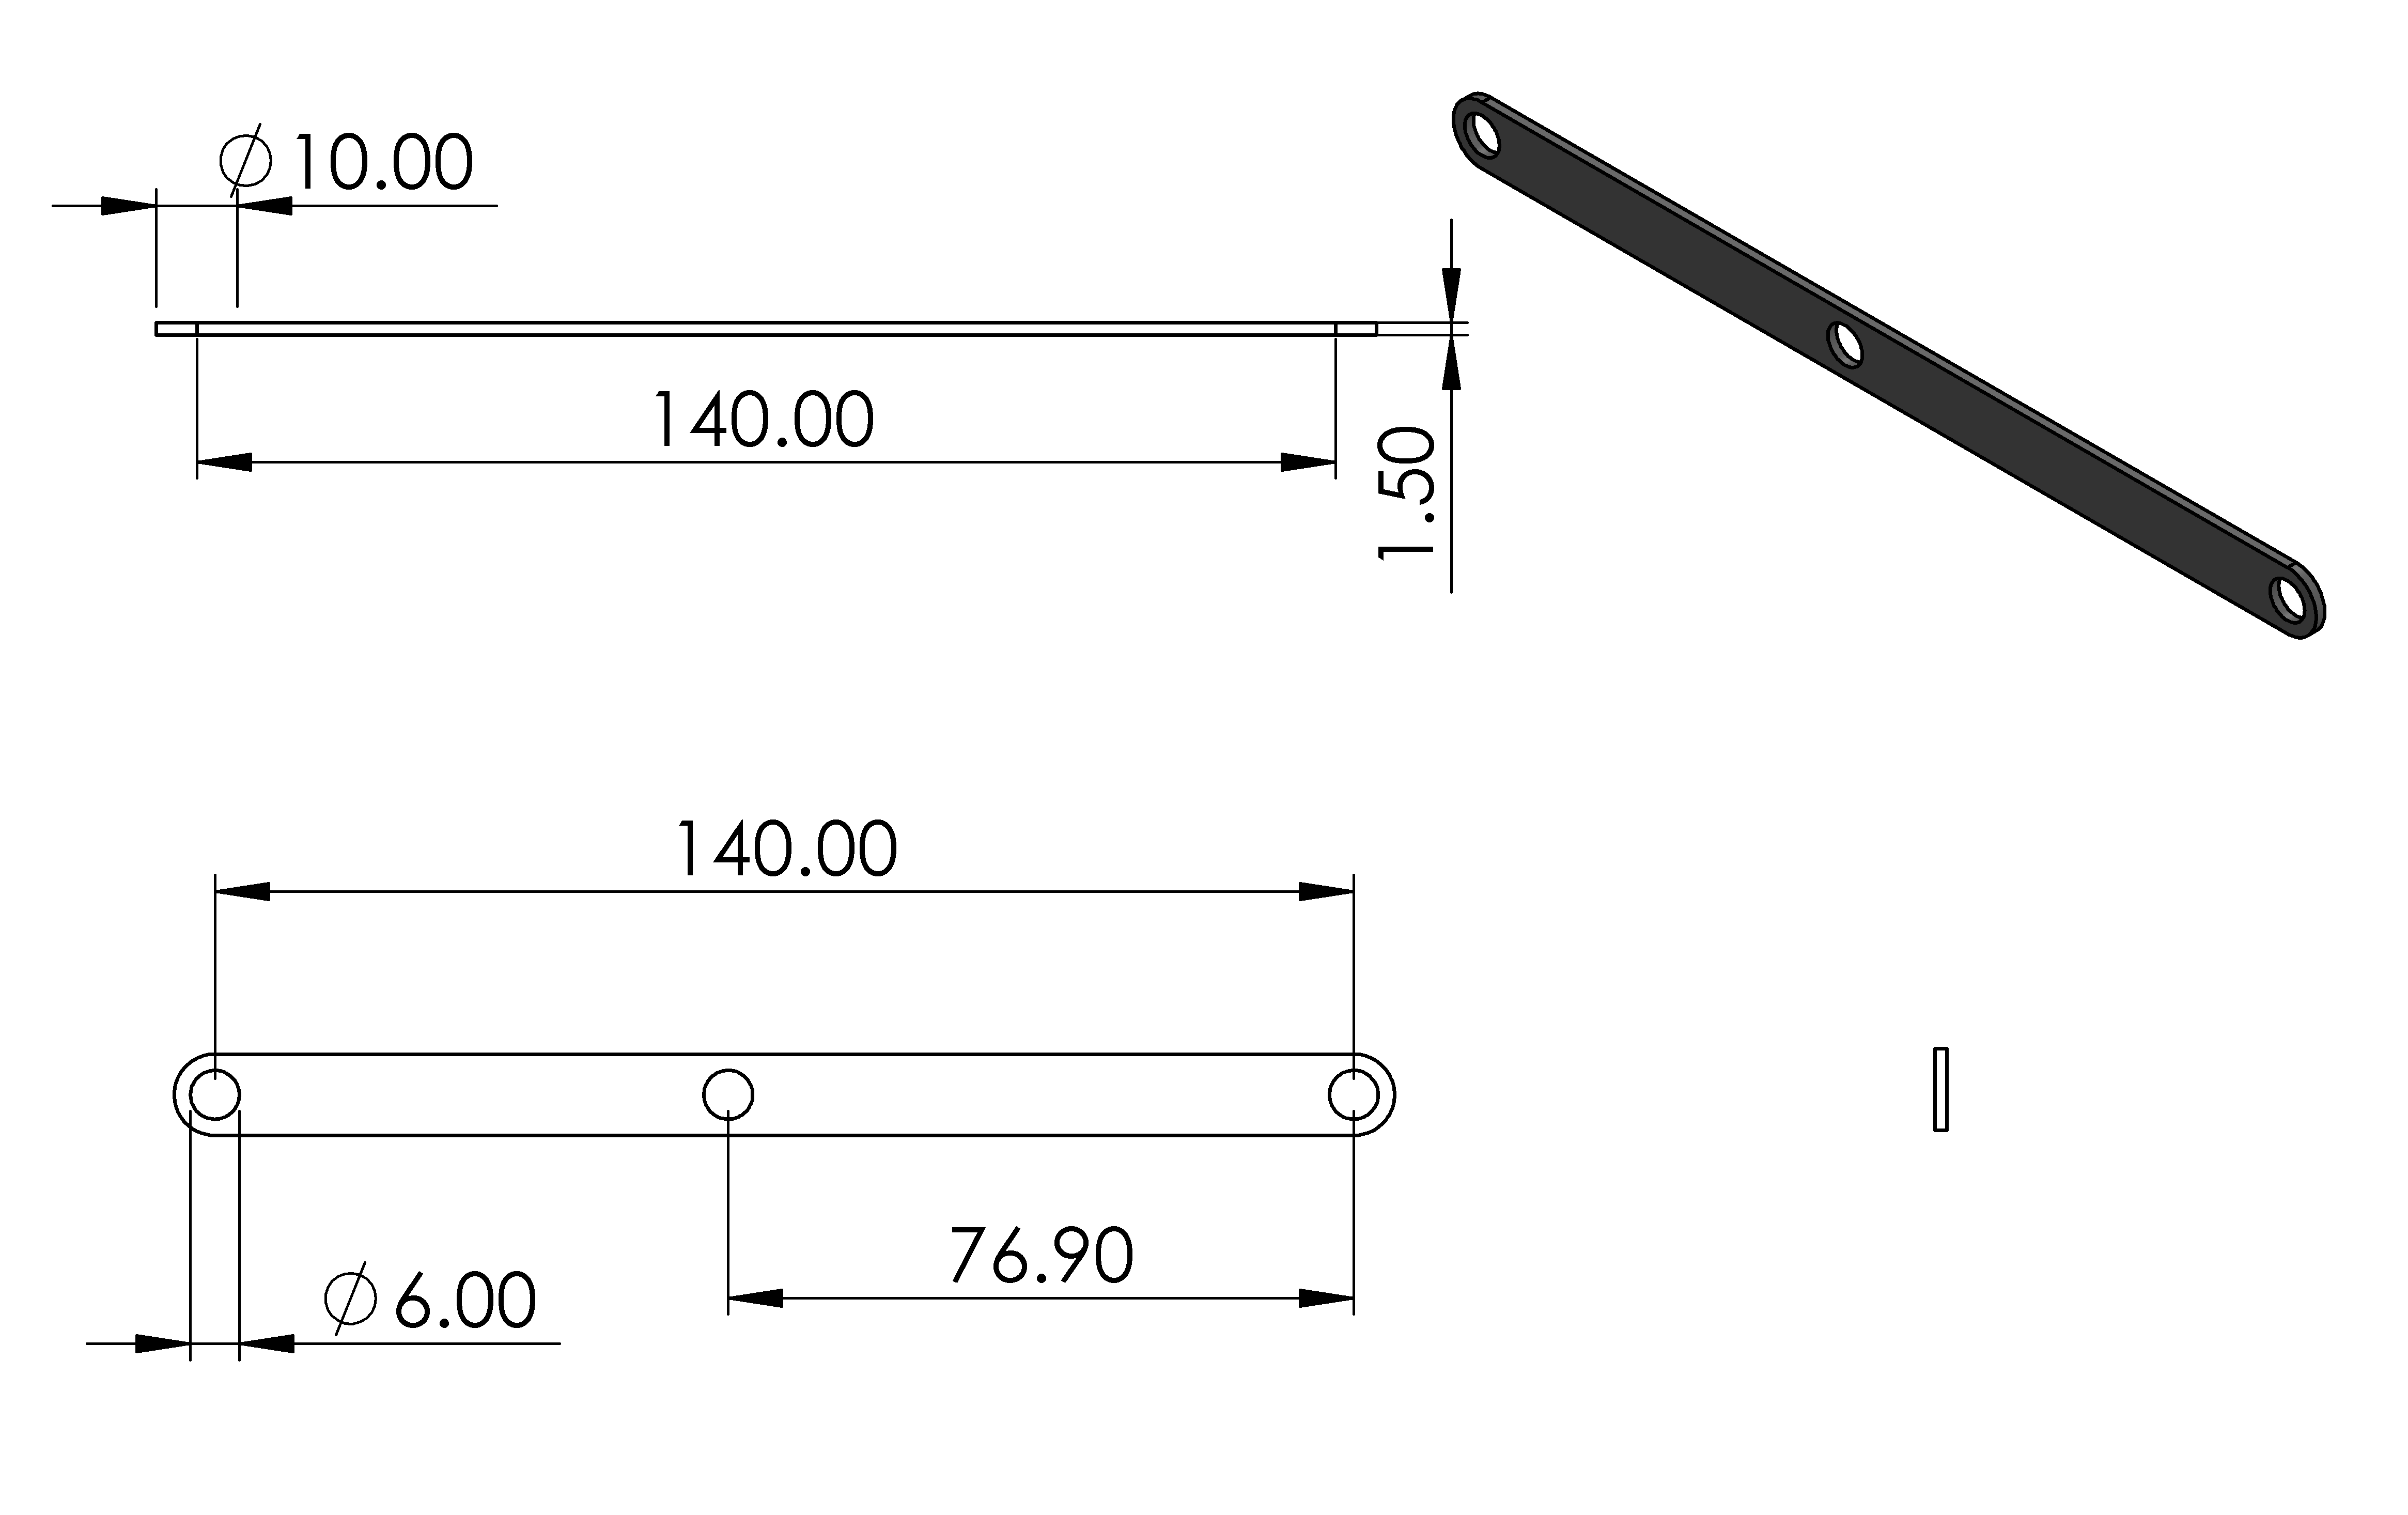
\includegraphics{Figures/KLink1.PNG}
            \caption{Coupler}
            \label{fig:coupler}
        \end{figure}
        The design is such that it hinges on an extension from the flap support frame on one end and connects to the rocker on the other end. The crank is connected at a distance from one end.
        \item \textbf{Rocker}
        \par
        The rocker connects to the coupler on one end and to the flap on the other end. Its design is as shown in figure \ref{fig:rocker}.
        \begin{figure}[H]
            \centering
            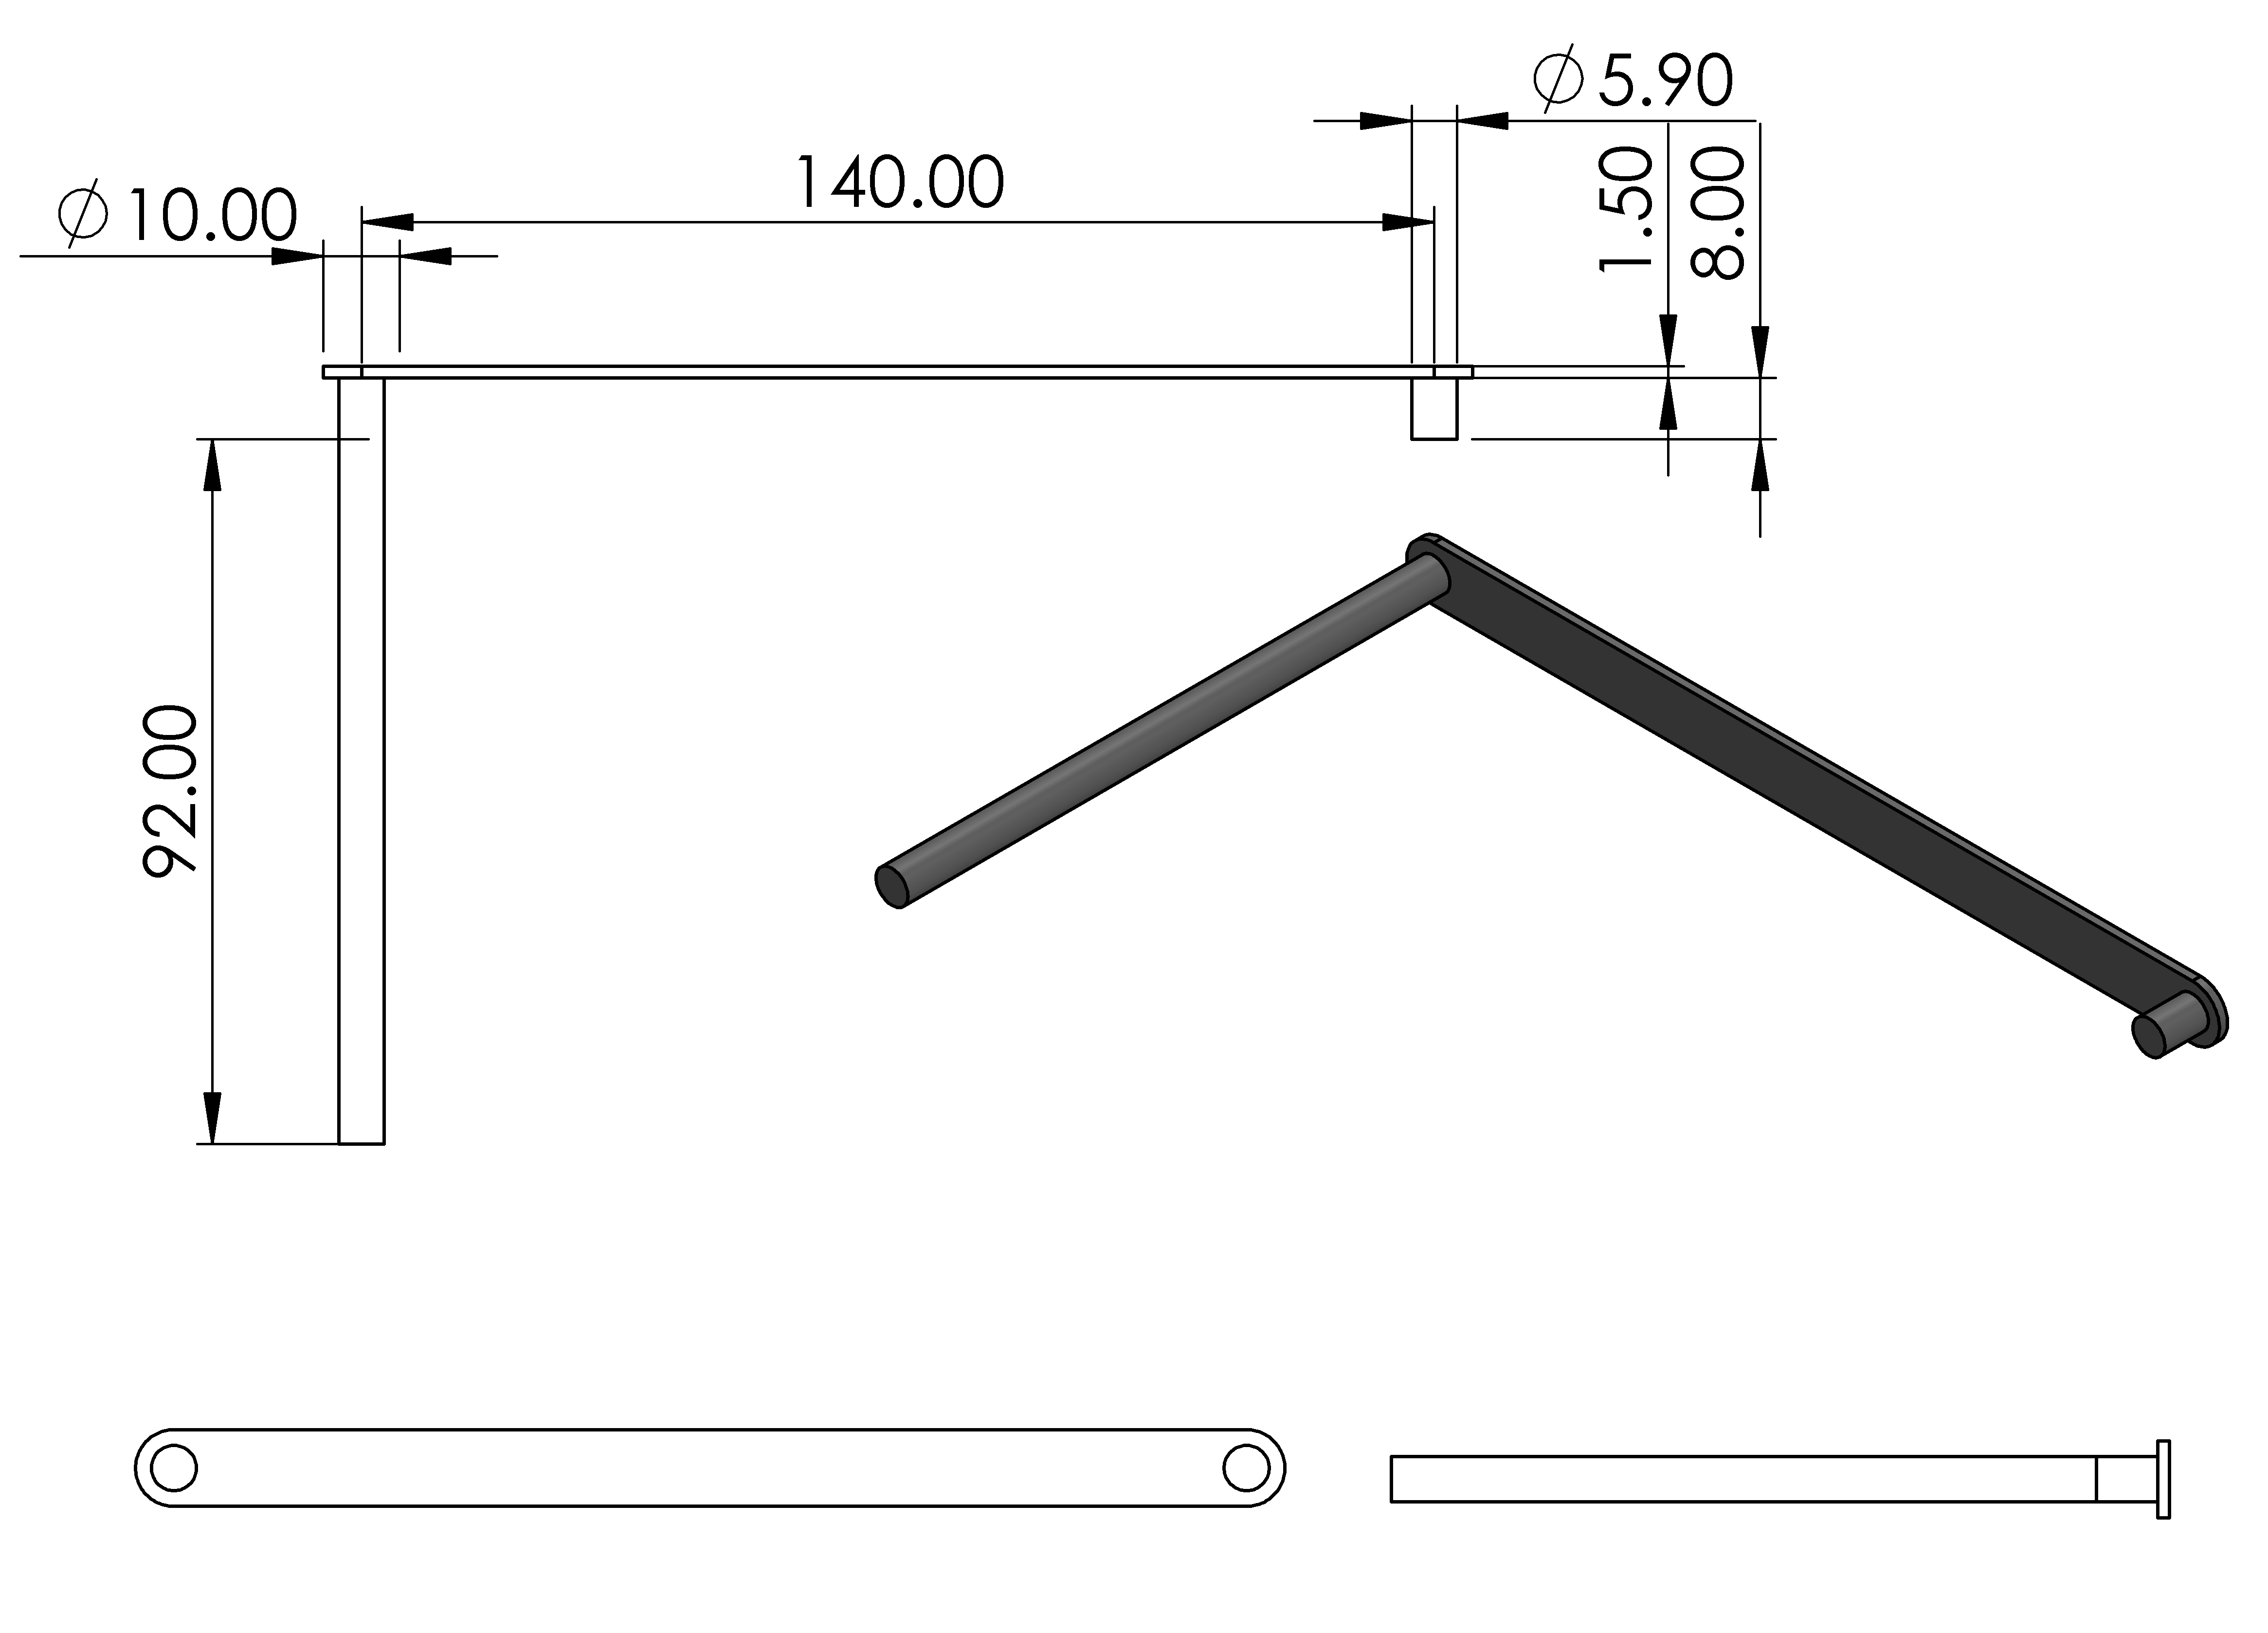
\includegraphics{Figures/KLink2.PNG}
            \caption{Rocker}
            \label{fig:rocker}
        \end{figure}
    \end{enumerate}
    \item \textbf{Discharge flow control sub-unit}
    \par
    In the assembly shown in Figure \ref{fig:flow_diversion_assembly}, the flap support frame hinges on two rods: one of the servo mount rods and the other is one of the legs of the electromagnetic holder.
    \begin{figure}[H]
        \centering
        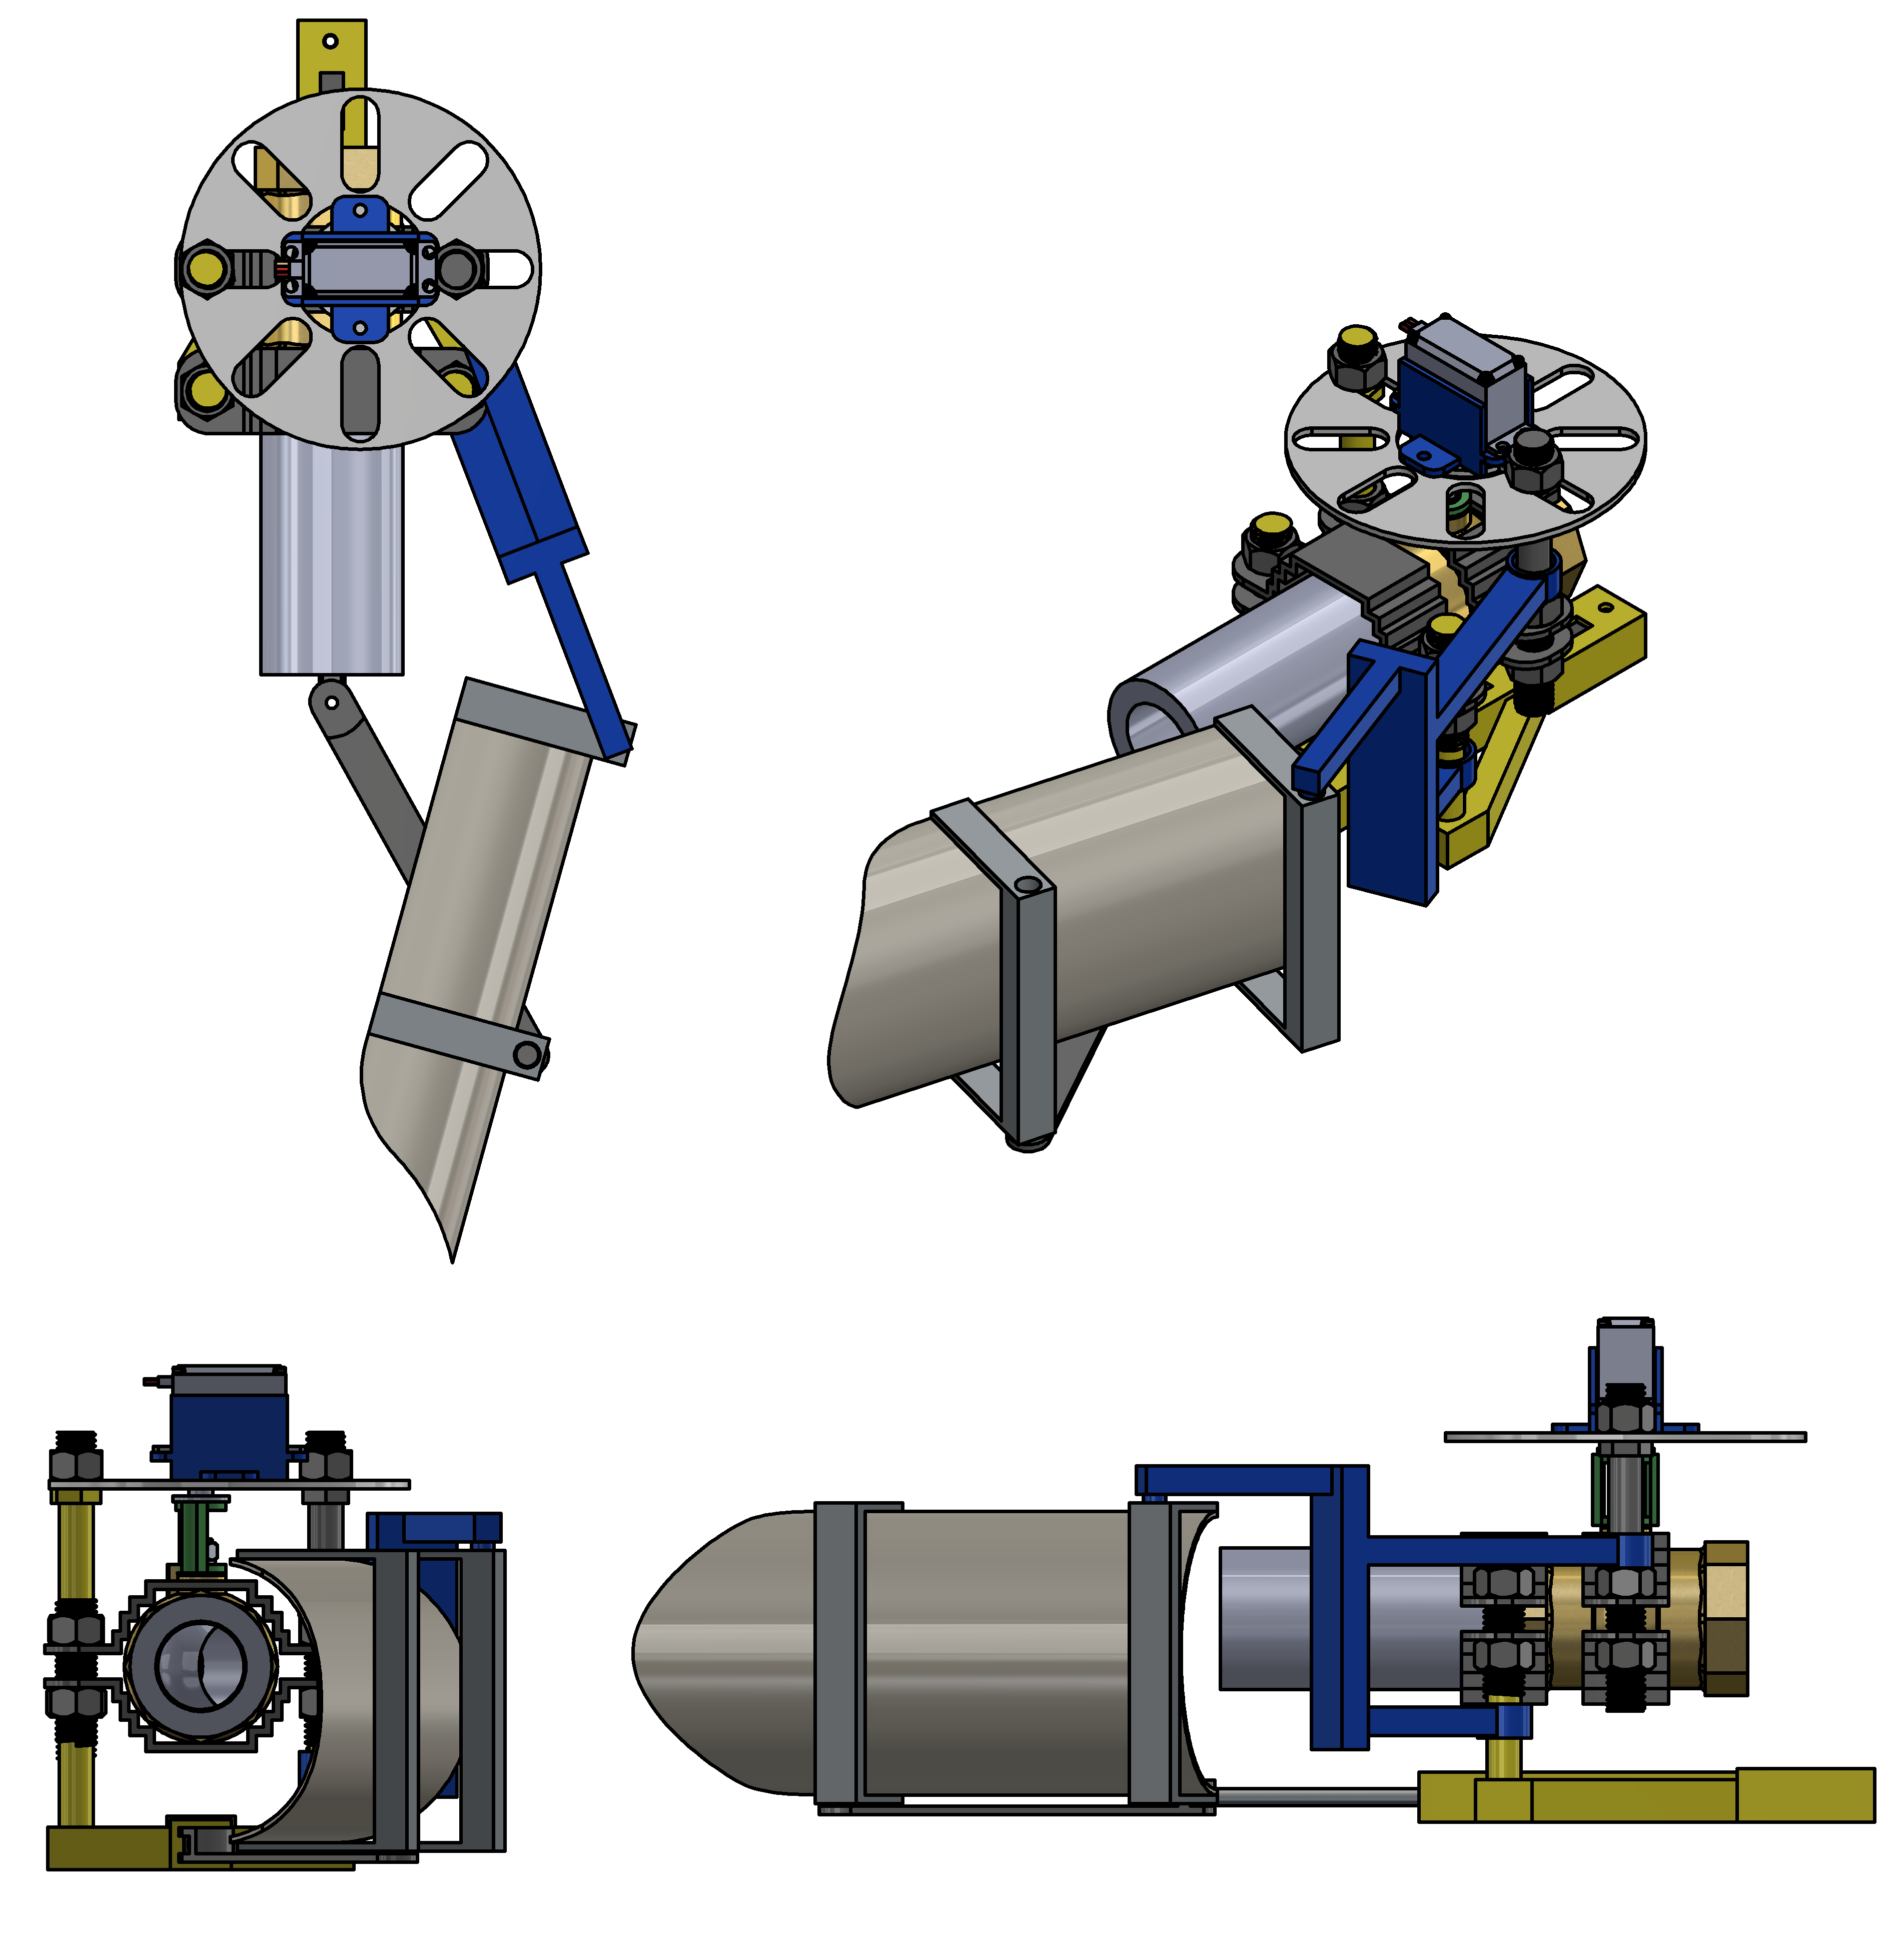
\includegraphics{Figures/DischargeFlowDiverSionAssembly.PNG}
        \caption{Flow Diversion assembly}
        \label{fig:flow_diversion_assembly}
    \end{figure}
    \item \textbf{Finite element analysis of the electromagnetic actuator assembly}
    \par
    The finite element analysis of the assembly was performed to test how the electromagnetic diversion system is stable under a pressure force of $1N/m^{2}$ applied to the inside of the flap. The results of the simulation are shown in figure \ref{fig:e_simulation_results}.
    \begin{figure}[H]
        \centering
        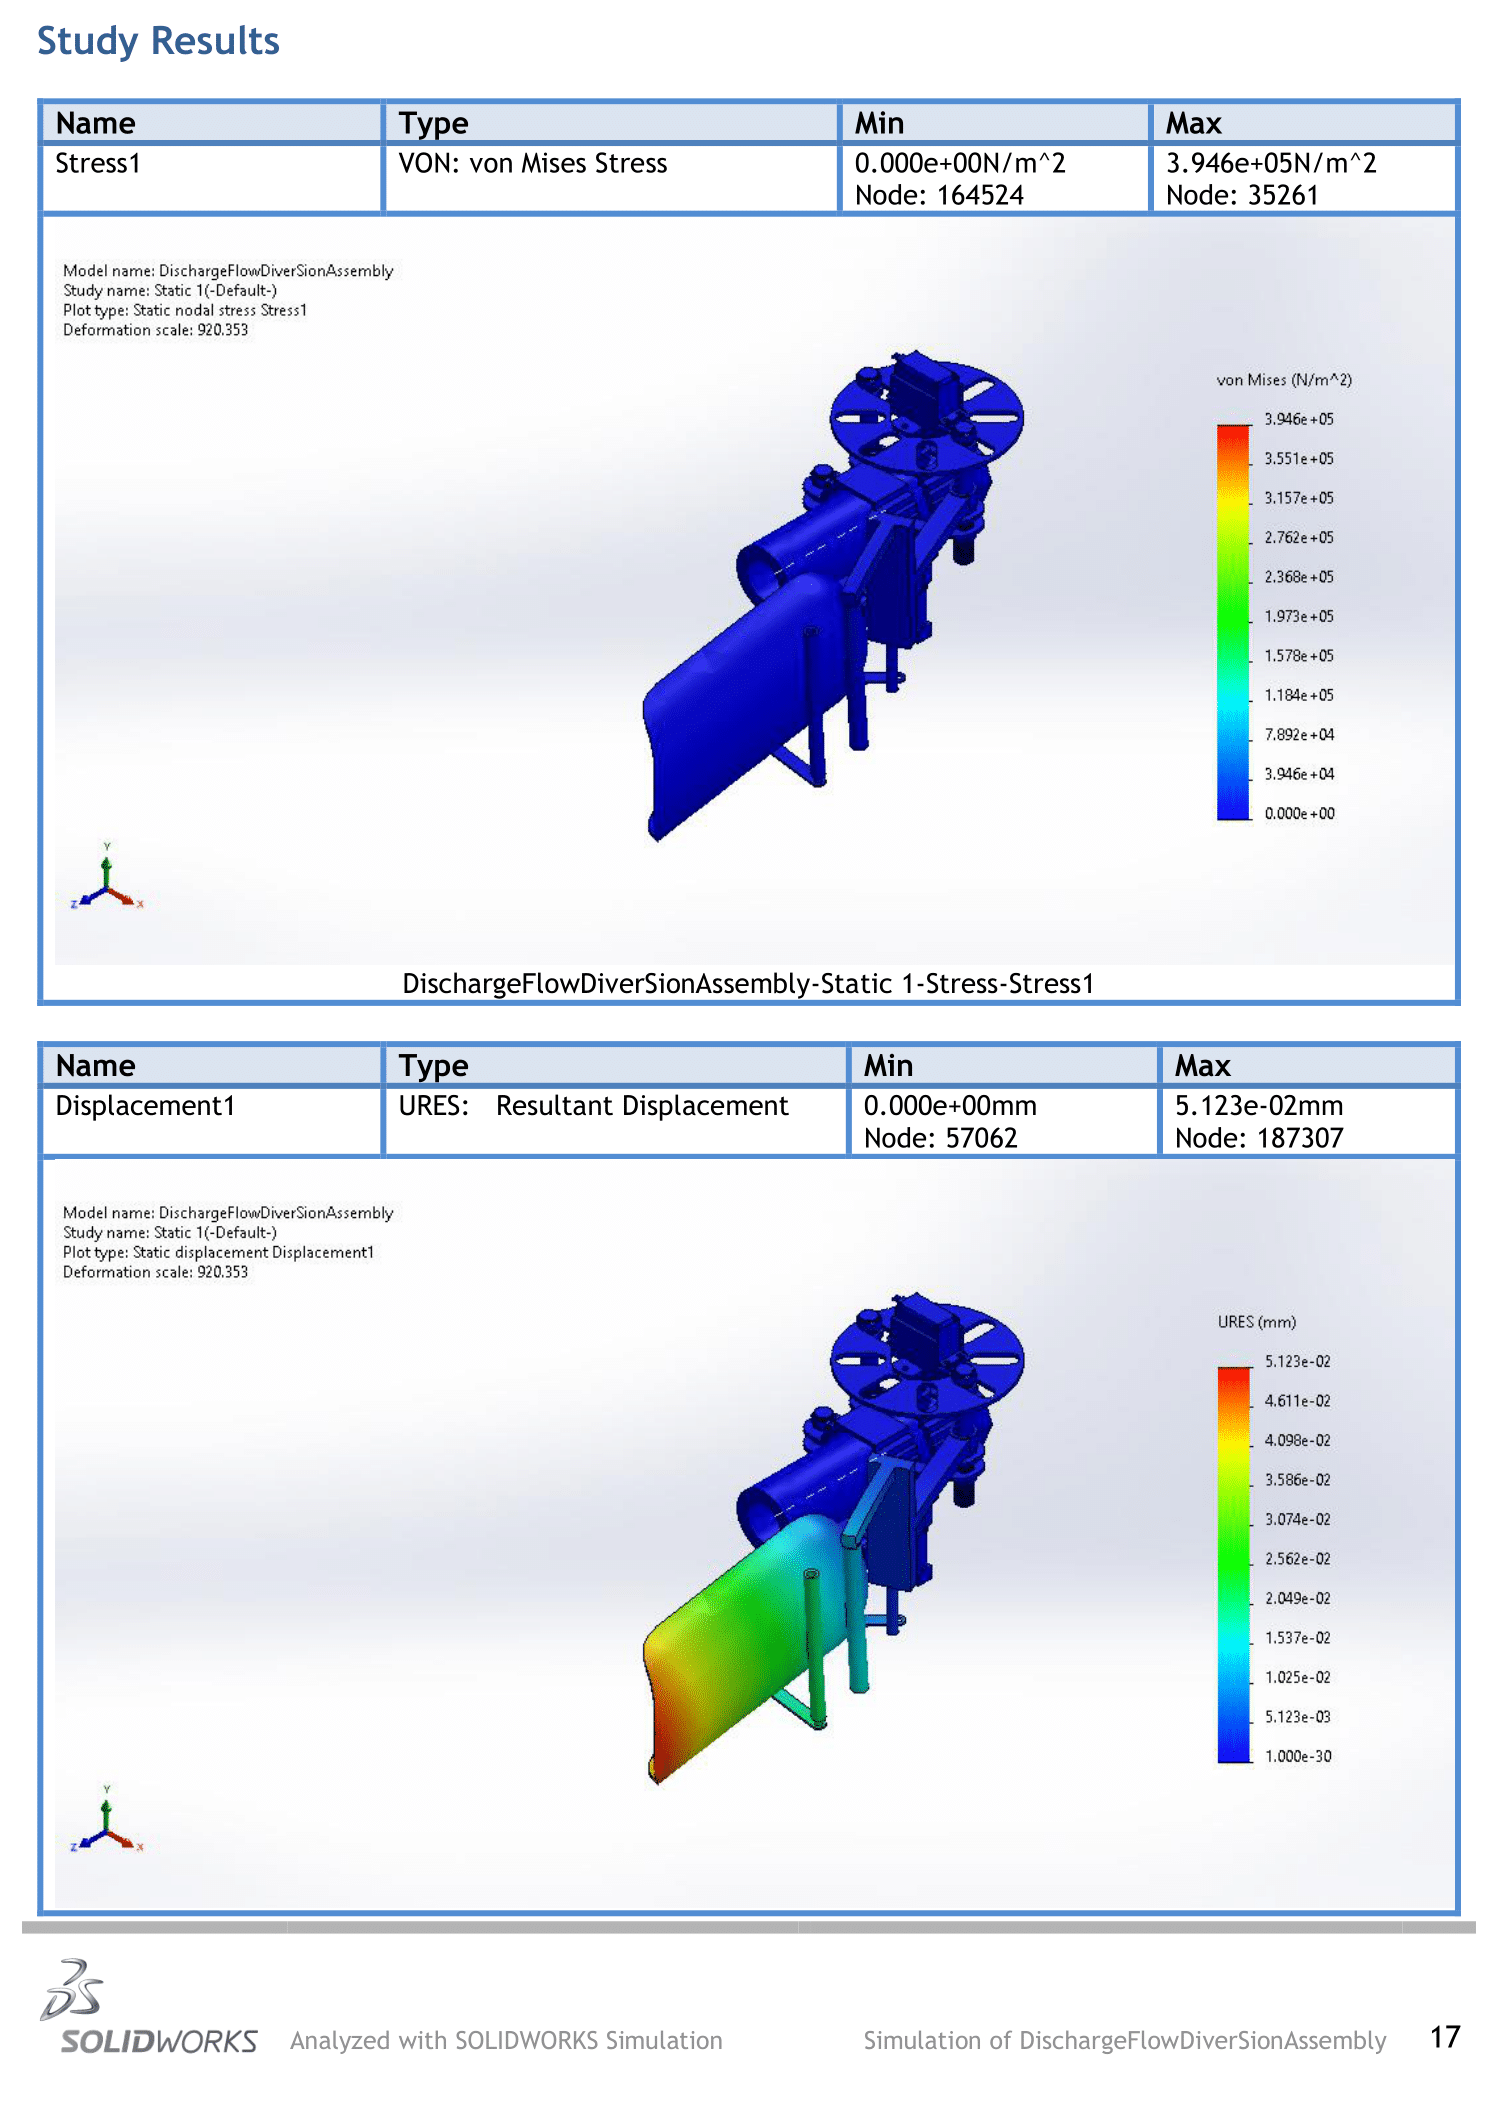
\includegraphics[height=\textheight, width=\textwidth]{Figures/DischargeFlowDiverSionAssembly-Static 1-1-1.png}
        \caption{Diversion assembly FEA results}
        \label{fig:e_simulation_results}
    \end{figure}
    From the results in figure \ref{fig:e_simulation_results}, it is evident that the electromagnetic actuator assembly holds up to the amount of distributed pressure on the flap. 
\end{enumerate}
\subsubsection{Electrical}
\begin{enumerate}
    \item \textbf{MG996R Servo motor connection}
    \par
    \begin{itemize}
        \item \textbf{Power requirements}
        \par
        From the technical specifications of the motor listed in table \ref{tab:MG996R_servo_specs}, this motor's operating voltage is 4.8V-7V, its driving current is between 500mA and 900mA, and its stall current is 2.5A(6V). However, most microcontrollers supply up to +5V DC voltage. This therefore requires a step-up circuitry or an external voltage supply to the  motor.
        \item \textbf{Connection}
        \par
        To connect an external supply requires a circuit shown in figure \ref{fig:servo_connection}.
        \begin{figure}[H]
            \centering
            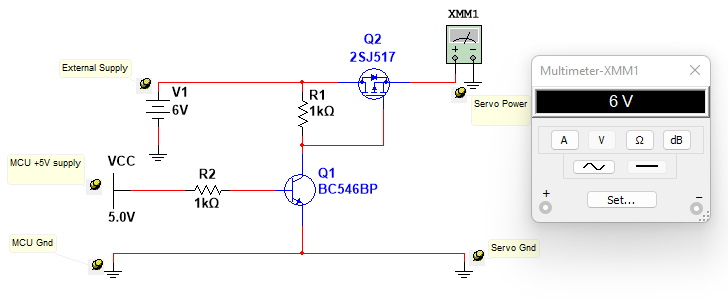
\includegraphics[width=\textwidth]{Figures/ServoConnection.png}
            \caption{Servo Connection}
            \label{fig:servo_connection}
        \end{figure}
        A 6V DC external supply is connected to the drain terminal of a Power MOSFET. This is activated by an NPN BJT transistor using the voltage supplied by the microcontroller.
    \end{itemize}
    
    \item \textbf{P16-S Electromagnetic Actuator connection}
    \par
    \begin{itemize}
        \item \textbf{Power requirement}
        \par
        The power requirements for this actuator are 12V DC supply and 2A current as listed in table \ref{tab:p16_s}. These two power requirements cannot be satisfied by just a micro-controller; an external source is necessary.
        \item \textbf{Connection}
        \par
        This two power requirement can be satisfied using a combination of a MOSFET power IRF520 and a D1 flyback diode as shown in Figure \ref{fig:electromagnet_connection}.
        \begin{figure}[H]
            \centering
            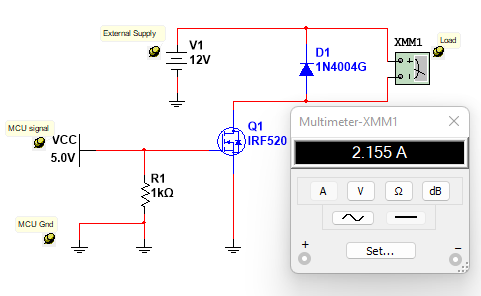
\includegraphics{Figures/ElectromagnetConnection.png}
            \caption{Electromagnetic Actuator circuit}
            \label{fig:electromagnet_connection}
        \end{figure}
        This is available in a module shown in figure \ref{fig:irf520_module}.
        \begin{figure}[H]
            \centering
            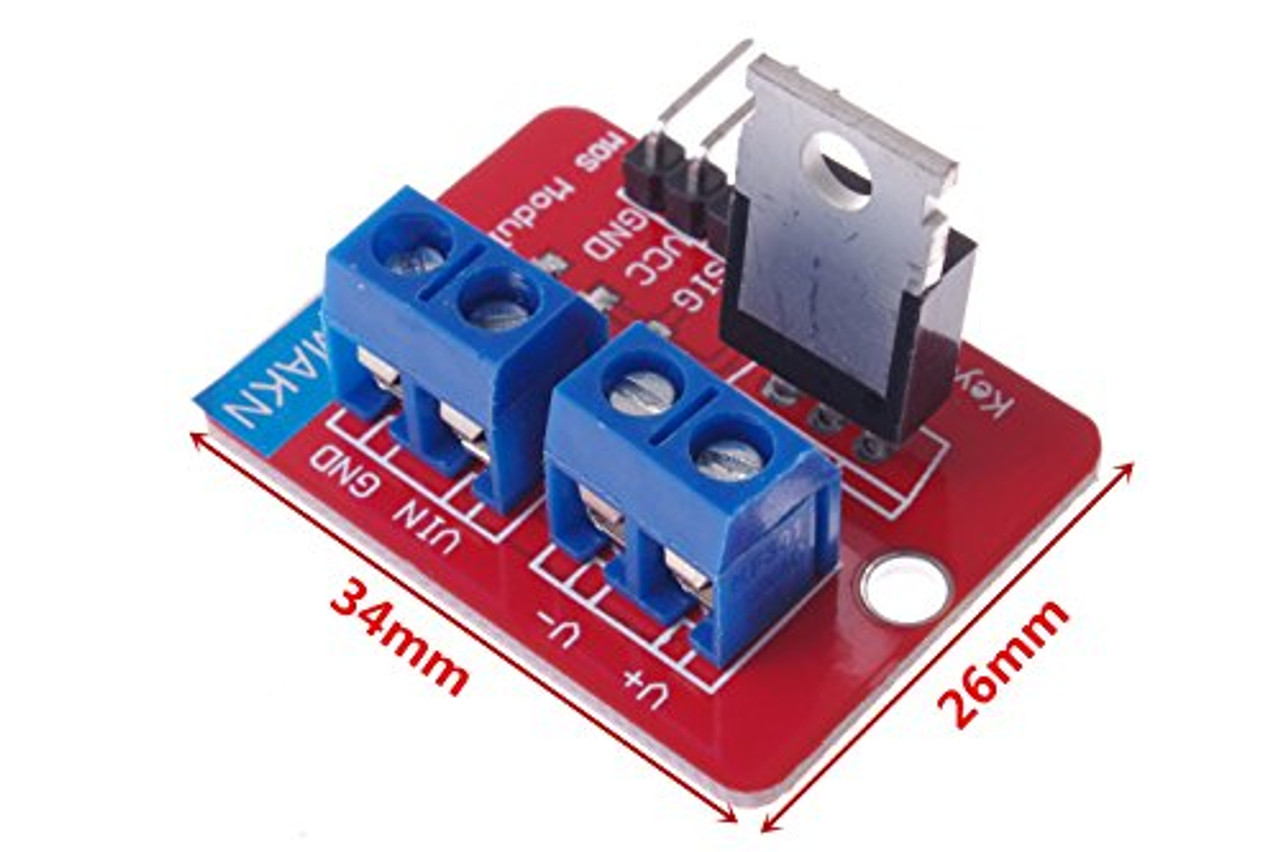
\includegraphics[width=.25\textwidth,height=.25\textheight]{Figures/IRF520Module.jpg}
            \caption[IRF520 Module]{IRF520 Module \cite{irf520}}
            \label{fig:irf520_module}
        \end{figure}
    \end{itemize}
\end{enumerate}
\subsubsection{Software and control}

\begin{enumerate}
    \item \textbf{MG996R Servo motor control}
    \par
    \begin{itemize}
        \item \textbf{Requirements}
        \par
        This motor is required to drive the ball valve in steps in a $90^{0}$ turn, the angle covered to close and open the ball valve. However, the motor can turn $120^{0}$. Therefore, the $90^{0}$ turn can be achieved by Pulse Width Modulation. 
        \item \textbf{Control}
        \par
        From the motor's datasheet, the period of the motor's control signal is 50Hz(20ms). This is checked against the clock frequency of the microcontroller and used to determine the prescaler value for the timer register.
        \par
        For example:
        \begin{align*}
            \text{Consider a micro-controller with clock frequency:} 84MHz \\
            Timer\_Frequency = Period \times PWM\_Frequency\\
            \therefore = 20000 \times 50 Hz  = 1MHz\\
            Pre-scaler = \frac{Clock\_frequency}{Timer\_frequency}\\
            \therefore = \frac{84}{1} = 84
        \end{align*}
        The angle turned by the motor is proportional to the Logic HIGH duty. Therefore, by writing a time value for $90^{0}$ full turn in the timer register, the turn can be achieved. Smaller turns can be achieved by writing corresponding time values to the timer register.
    \end{itemize}
    \item \textbf{P16-S electromagnetic Actuator control}
    \par
    \begin{itemize}
        \item \textbf{Requirements}
        \par
        In order to divert the flow, this actuator is required to provide a linear stroke and remain in position for a set amount of time. When the time elapse, it is required to linearly retract in order to restore the flow. 
        \item \textbf{Control}
        \par
        This actuator provides a full length stroke in;
        \begin{align*}
            \text{Full length of a stroke: } = 100mm\\
            Stroke\_speed = 150mm/s\\
            \therefore \text{Time taken for a full length stroke is} \frac{10}{15}^{th}  \text{of a second.}
        \end{align*}
        This is achieved when it is powered. The terminals are switched in order to retract it.
        \par
        Shorter strokes can be achieved by turning on the actuator for a time less than $\frac{10}{15}$ \textit{th} seconds.
    \end{itemize}
\end{enumerate}
Controlling these two electronics requires an RTOS platform. There are many RTOS platforms but Zephyr and Mbed platforms are preferred because of their relatively large support with extensive APIs. 
\clearpage
\subsection{Discharge Handling Unit}
This unit consists of the following subunits:
\begin{enumerate}
    \item Discharge collection tank sub-unit.
    \item Outlet valve sub-unit.
    \item Weight measurement sub-unit.
    \item Temperature measurement sub-unit.
\end{enumerate}

\subsubsection{Discharge collection tank sub-unit}
\begin{itemize}
\item \textbf{Collection tank}
\par
This is used to temporarily collect the discharge from the pipeline during each step of an experiment, after which it is released to the main reservoir through an outlet valve. The weight and temperature of the discharge are also taken in this tank. 
\par
The following design considerations were made when selecting a tank for this application.
\begin{enumerate}
    \item Shape of the tank 
    \par
    The design of this tank should be such that the tank discharges in the least time possible with no remnants. Therefore, the shape of the tank was put into much consideration such that it influences/motivates the discharge. This consideration was made in tandem with the consideration of the position of the outlet valve.
    
    \item Material of the tank
    \par
    The collection tank will hold water with chlorine chemicals. This brings about the thread of rust. Therefore, the tank material was chosen so that it minimises this thread. 
    \item Volume of the tank
    \par
    The volume of the tank tank was such that it can hold a stream from the $1 \frac{3}{4} inch$ main discharge pipe that flows for approximately 30 seconds when the valve is fully opened. This was around $0.01m^{3}$. Therefore, the dimensions of the tank were such that it produced a volume of this value.
\end{enumerate}
Based on the above considerations, two options were technically feasible in terms of the available means for fabrication:
\begin{enumerate}
    \item \textbf{Cuboid tank}
    \par
    The design of the tank is shown in Figure \ref{fig:cuboid_discharge_container}.
    \begin{figure}[H]
        \centering
        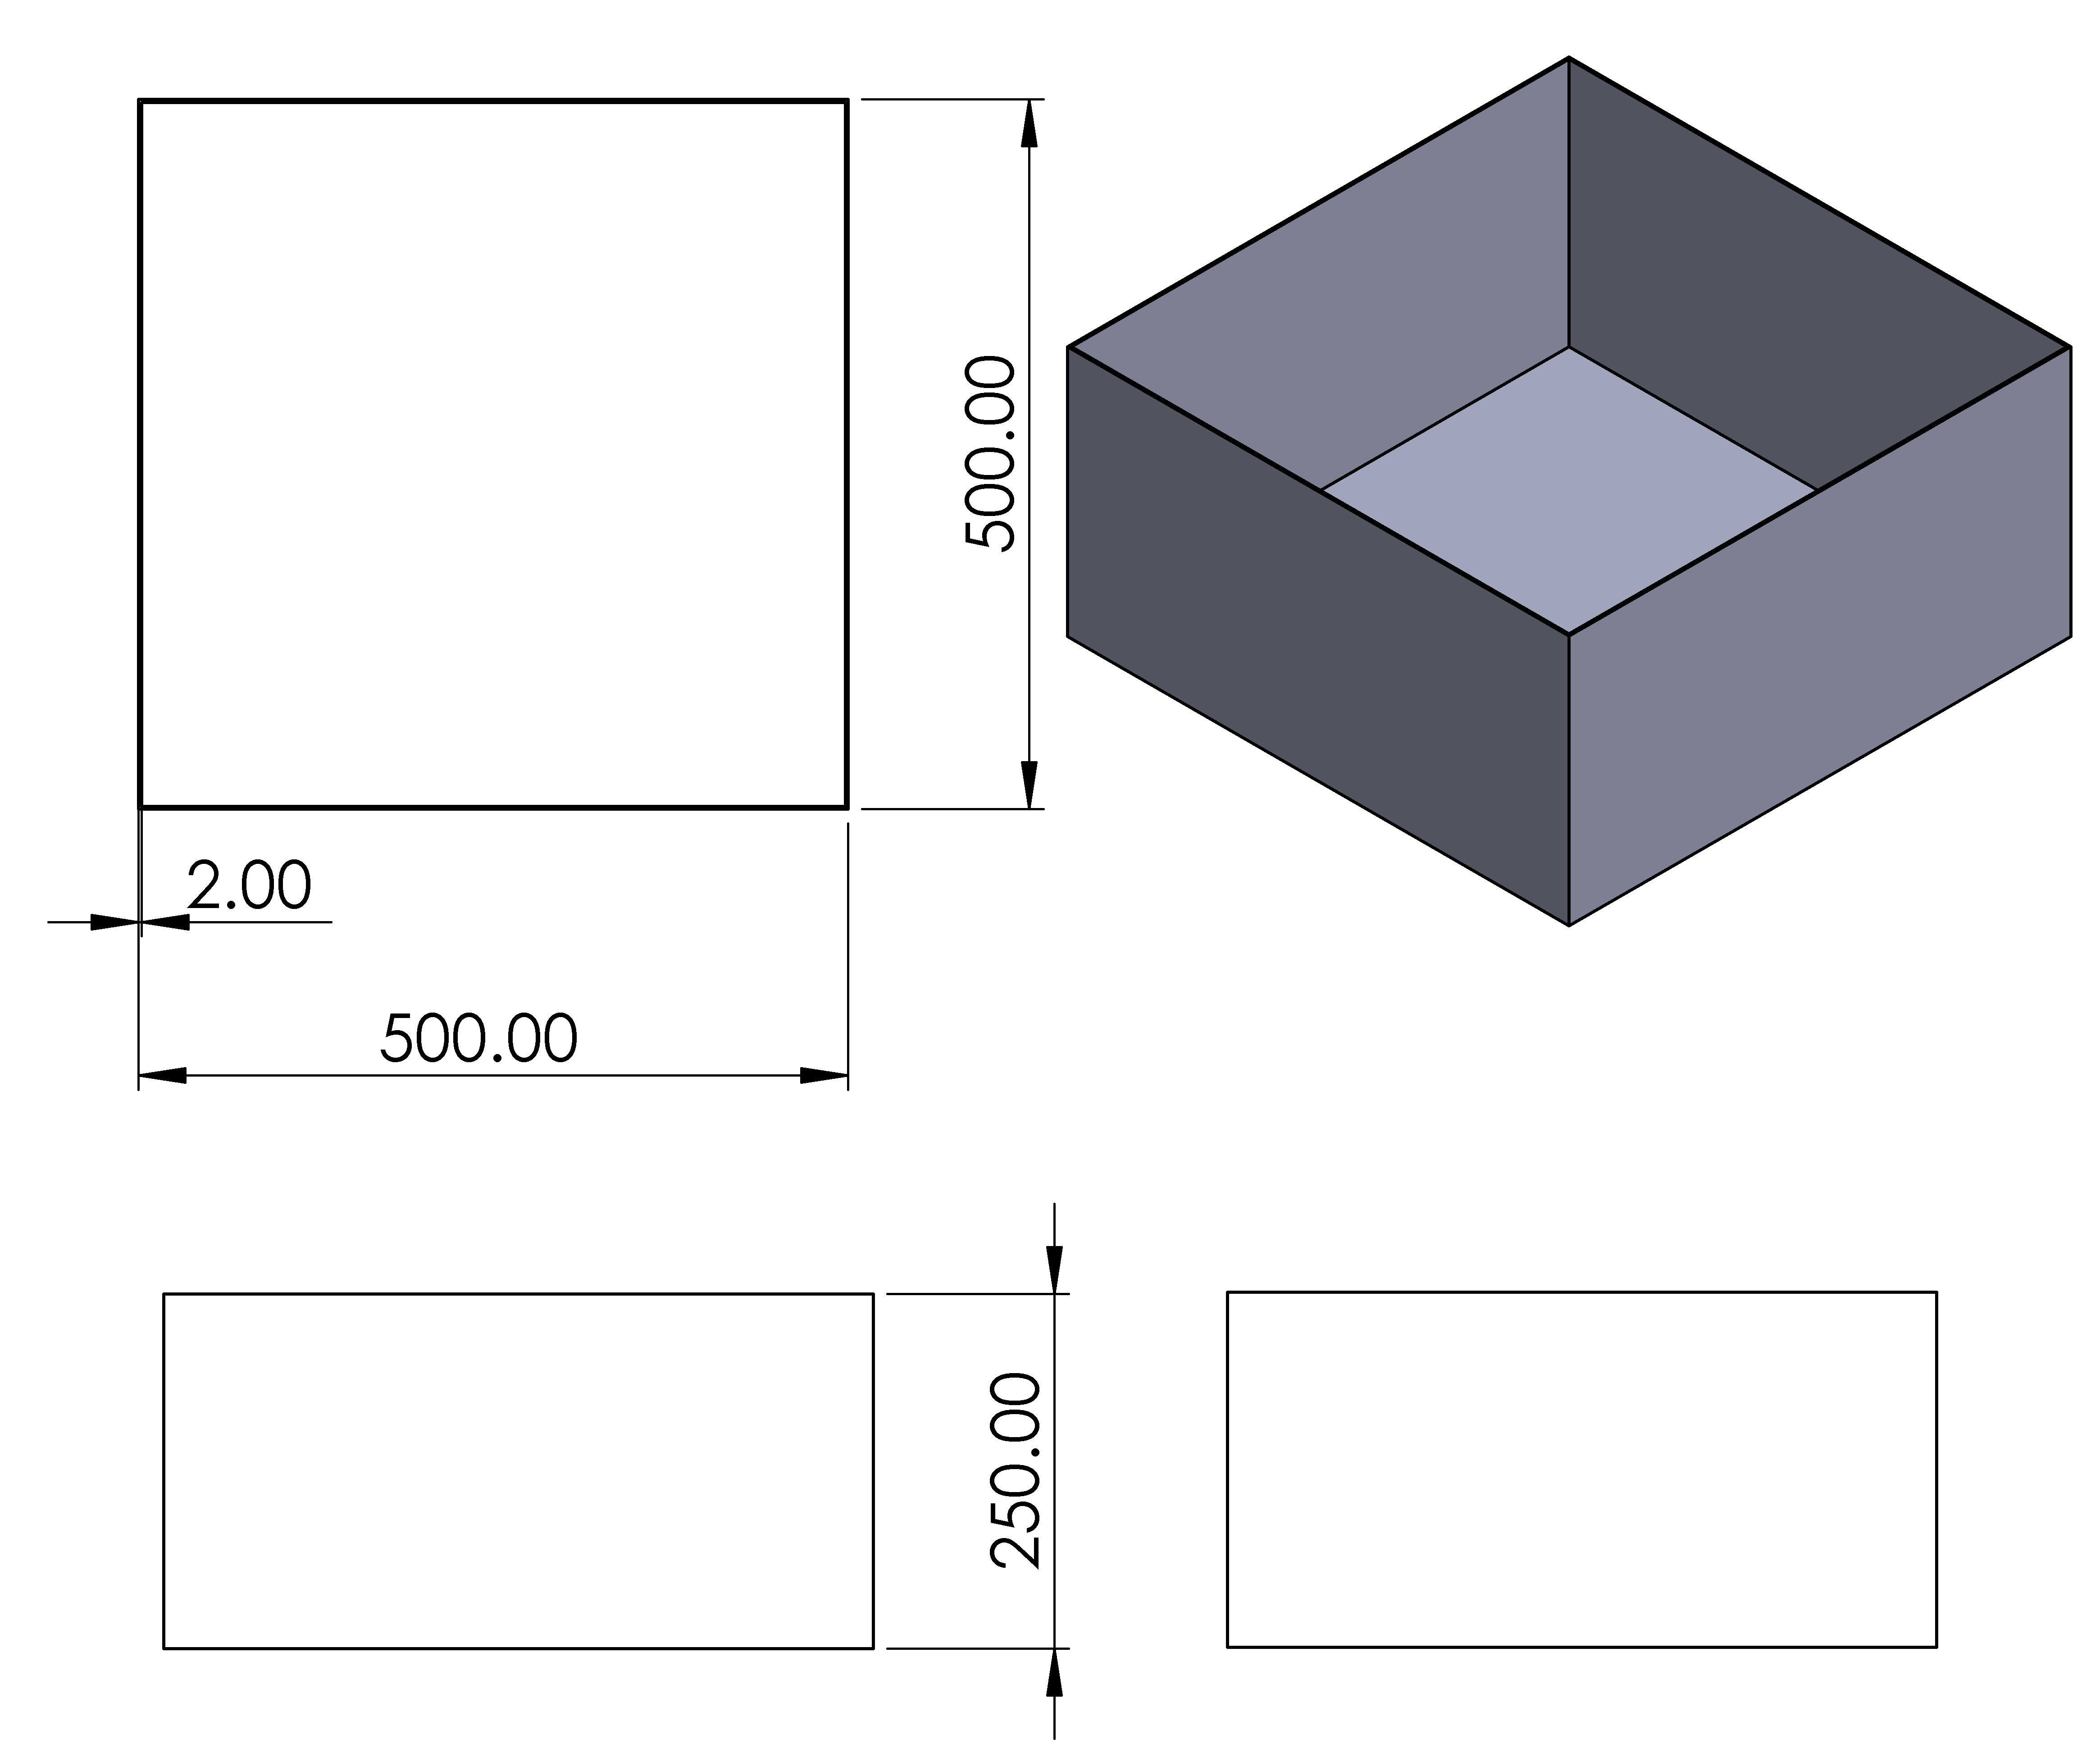
\includegraphics{Figures/DischargeContainer.PNG}
        \caption{Cuboid discharge container}
        \label{fig:cuboid_discharge_container}
    \end{figure}
    This tank satisfies the requirements for this application. However, a small volume of discharge will tend to remain in the tank when the tank is emptied.
    \item \textbf{Horizontal Cylindrical tank}
    \par
    The design of this tank is shown in Figure \ref{fig:horizontal_cylindrical_tank}.
    \begin{figure}[H]
        \centering
        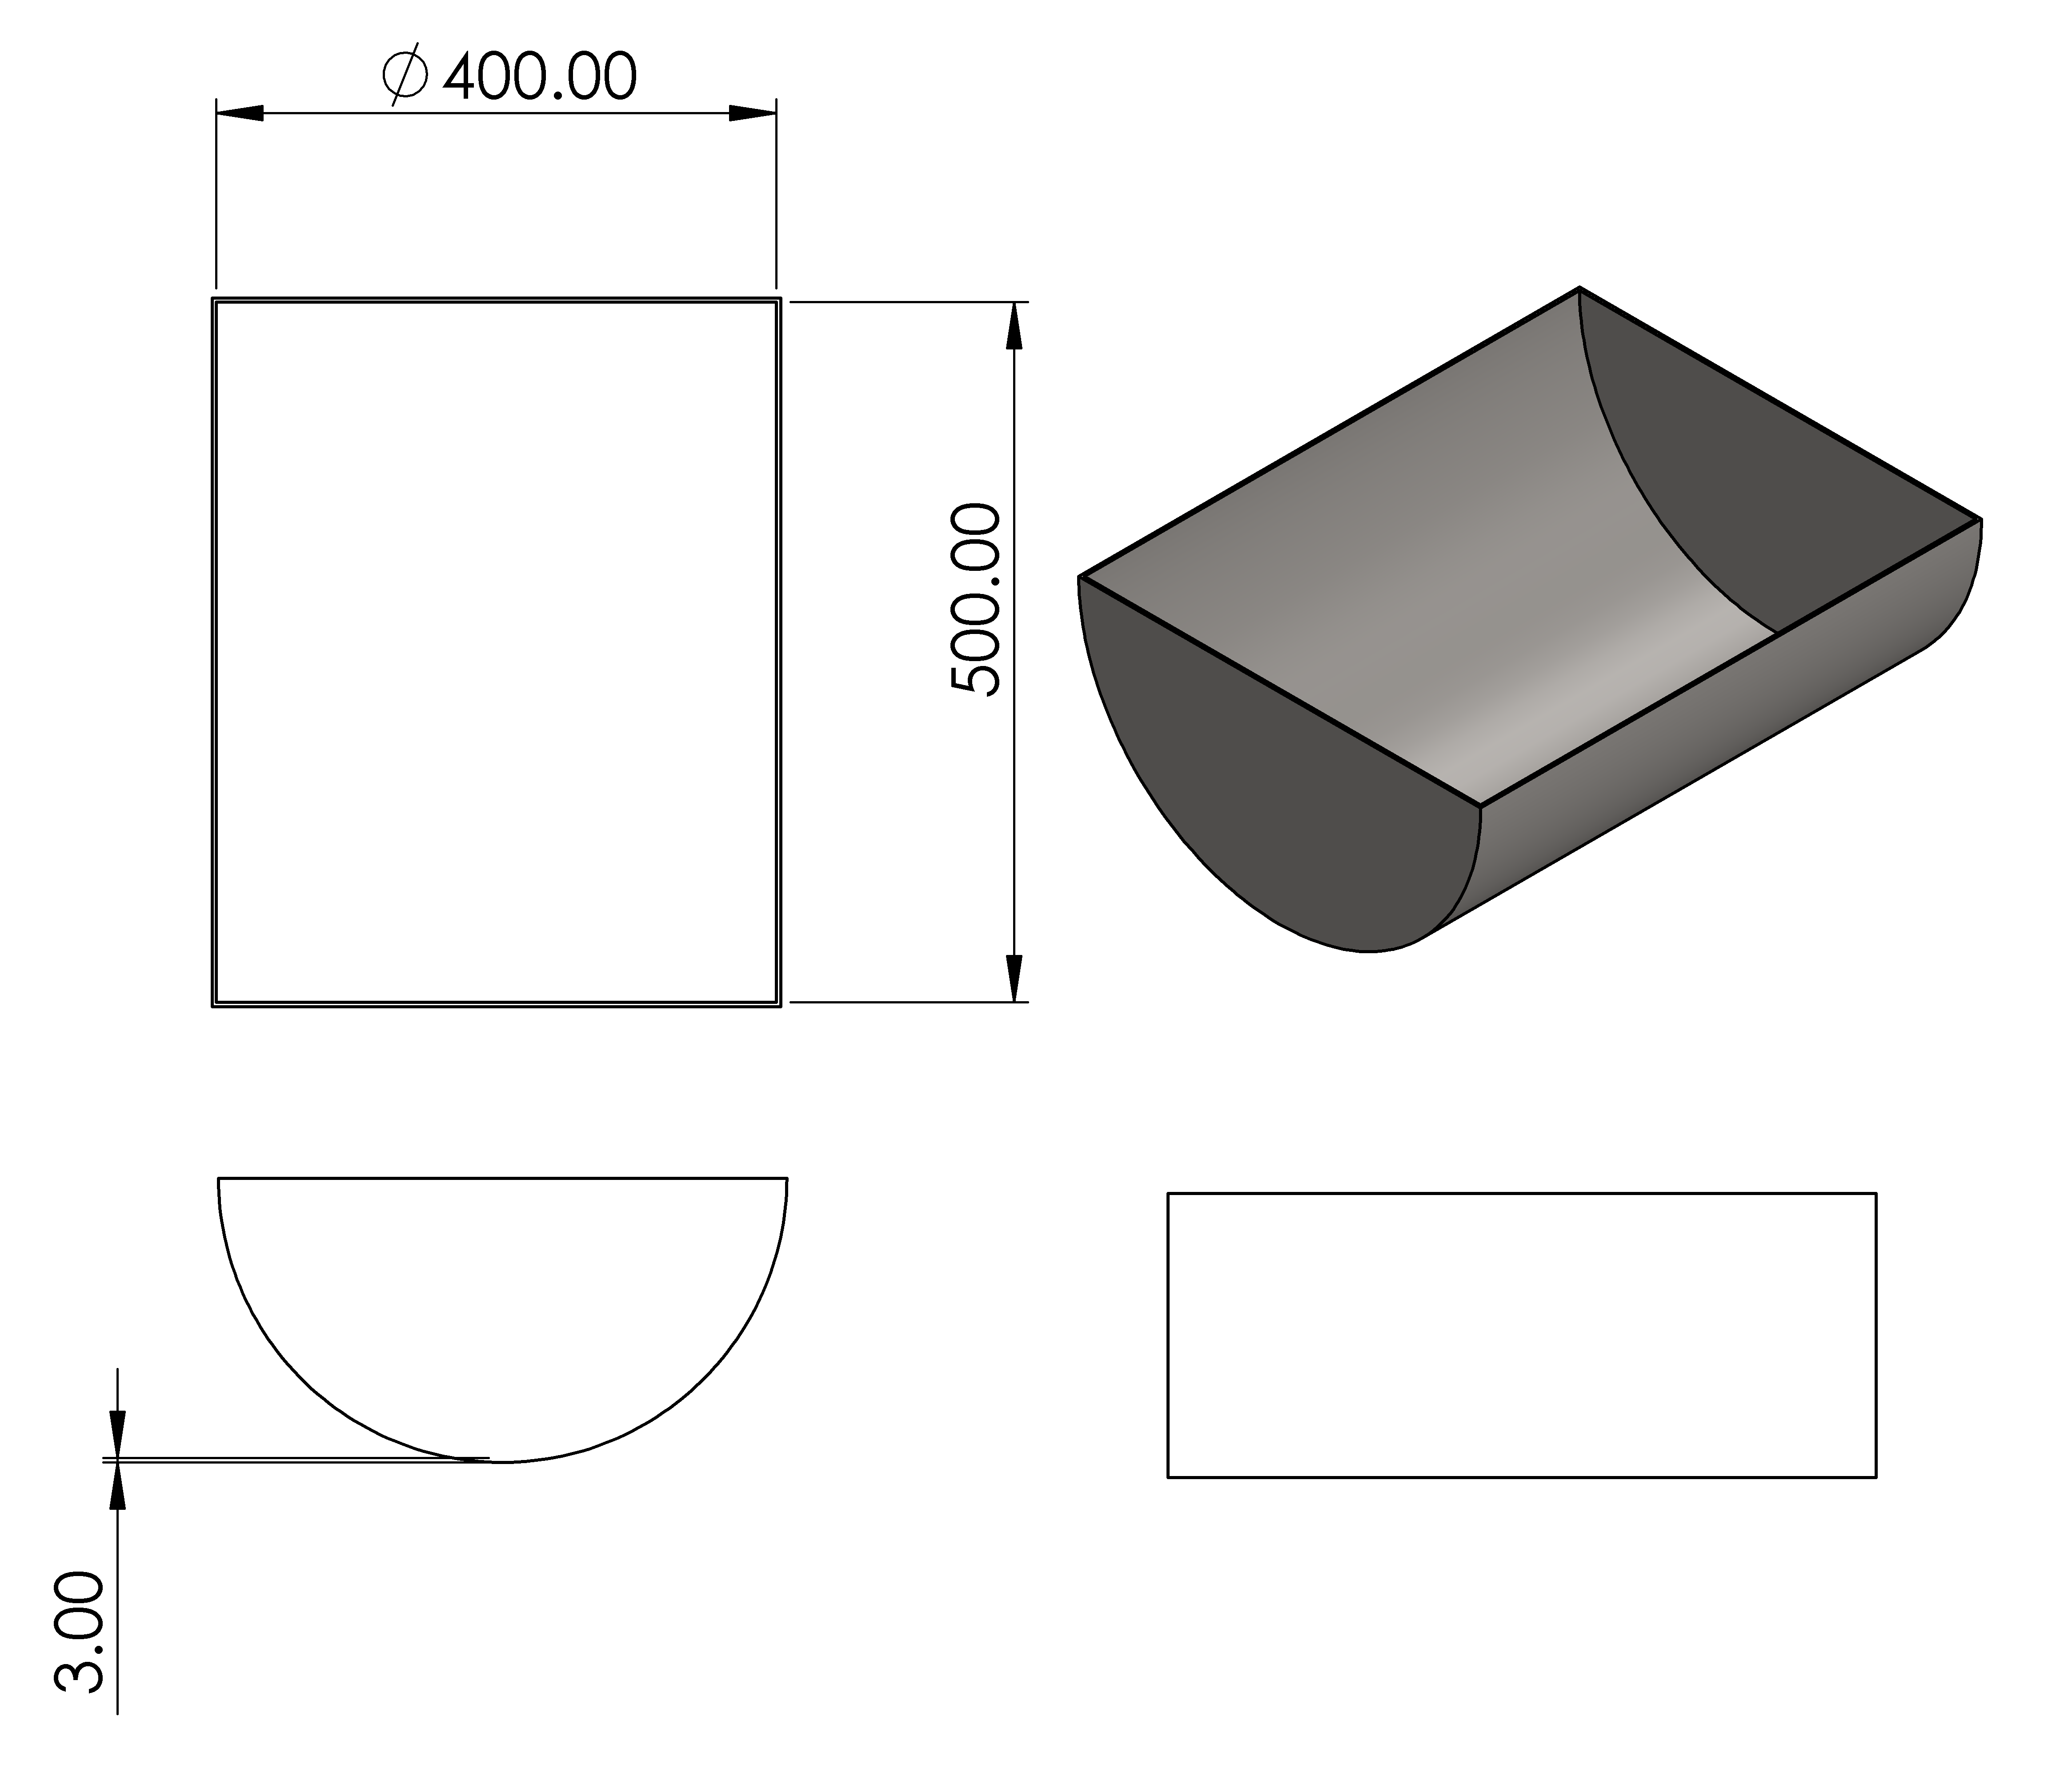
\includegraphics{Figures/tank2.PNG}
        \caption{Horizontal Cylindrical tank}
        \label{fig:horizontal_cylindrical_tank}
    \end{figure}
    When emptying this tank, the tank motivates the flow out of the discharge due to the concentration of the pressure of the discharge on a line at the bottom of the container, as shown by the results of the study simulation in Figure \ref{fig:tank_simulation_results}.
    \begin{figure}[H]
        \centering
        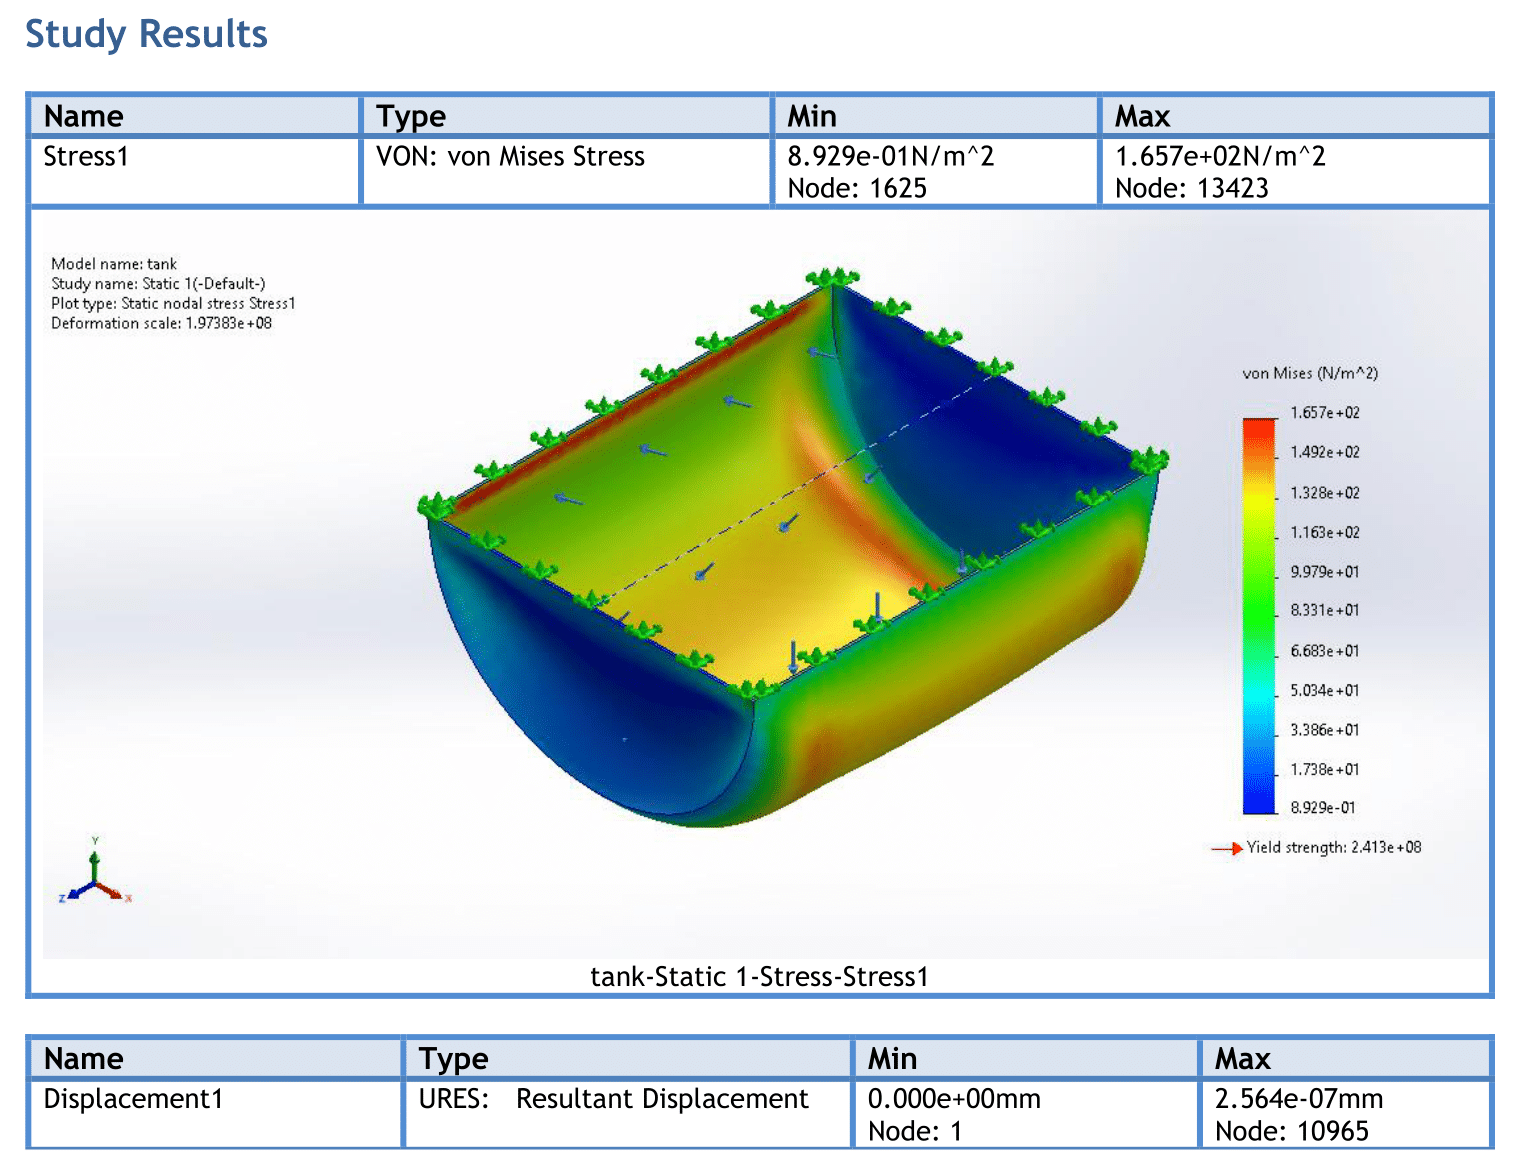
\includegraphics[width=\textwidth]{Figures/tank-Static-1-1-1.png}
        \caption{Tank simulation results}
        \label{fig:tank_simulation_results}
    \end{figure}
\end{enumerate}

The horizontal cylindrical tank was selected for this application.
\par
\item \textbf{Tank support frame}
\par
In order to support the tank in an upright position on a flat surface a support frame shown in figure \ref{fig:cylindrical_tank_support_frame}.

\begin{figure}[H]
    \centering
    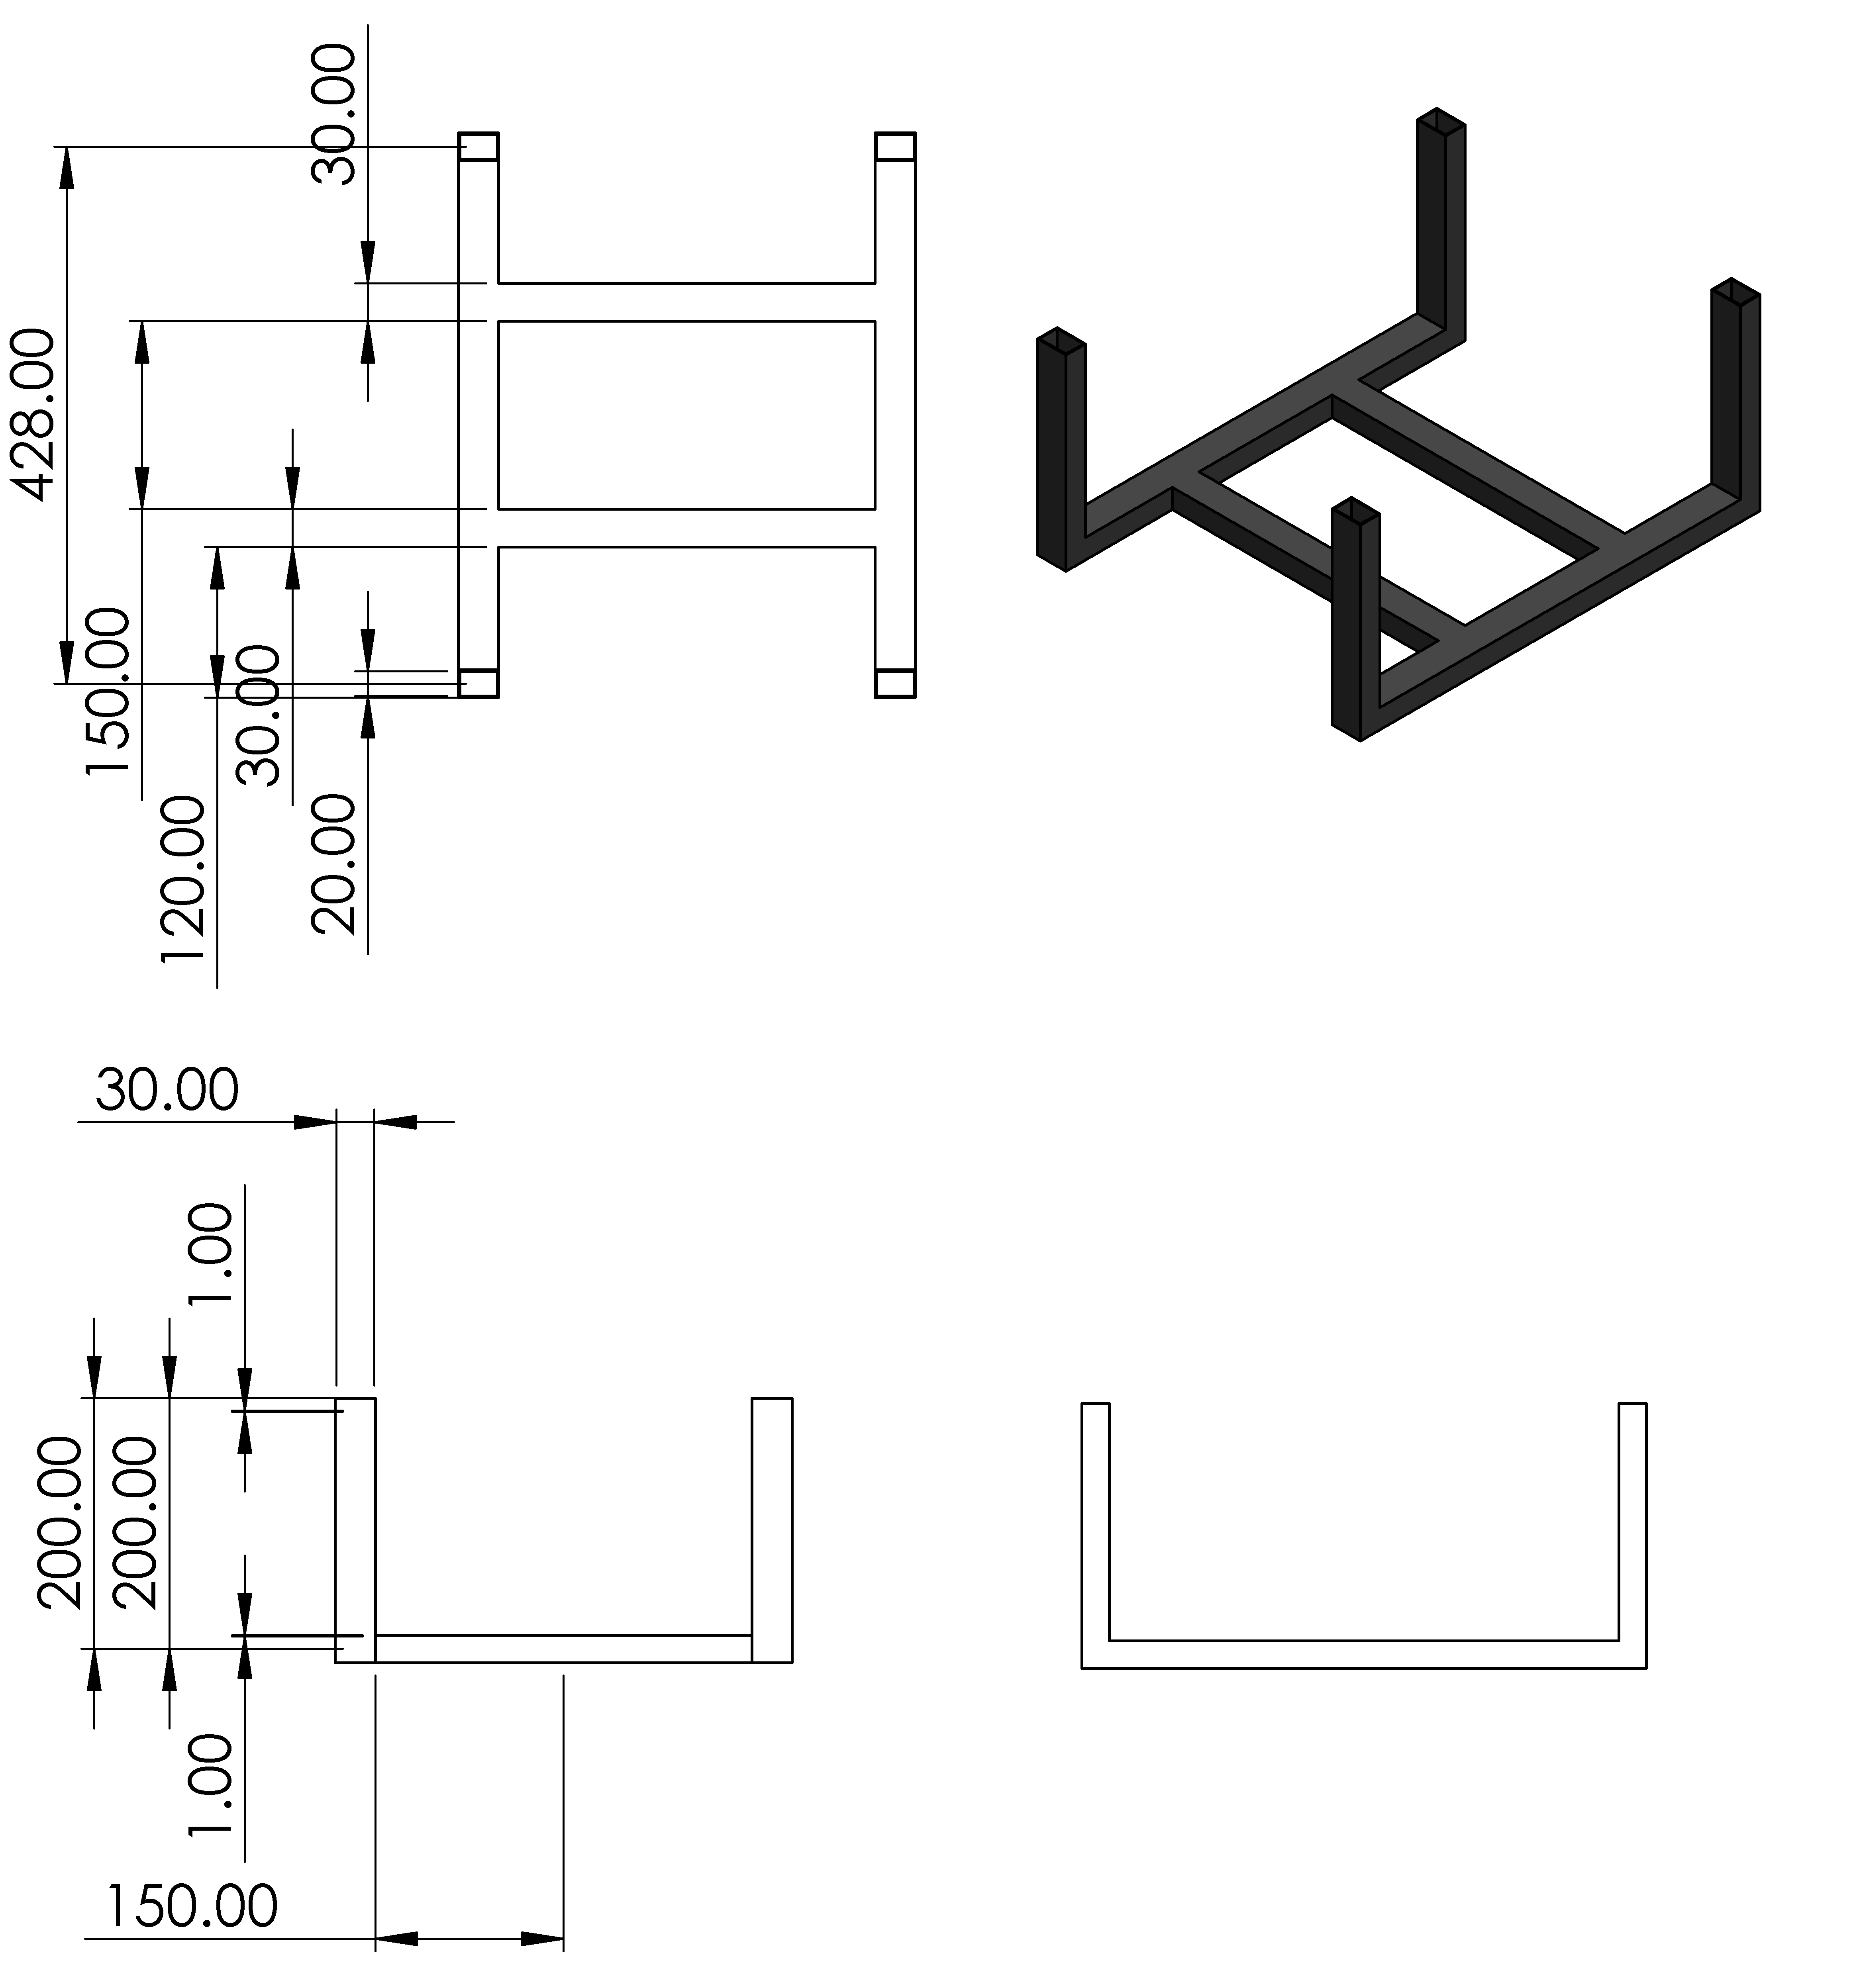
\includegraphics{Figures/tankHolder.PNG}
    \caption{Cylindrical tank support frame}
    \label{fig:cylindrical_tank_support_frame}
\end{figure}

The dimensions of the frame were such that it provides a clearance of 1mm for the tank.

\par
\item \textbf{Tank assembly}
\par
The assembly of the tank and its support frame are as shown in figure \ref{fig:collection_tank}.
\begin{figure}[H]
    \centering
    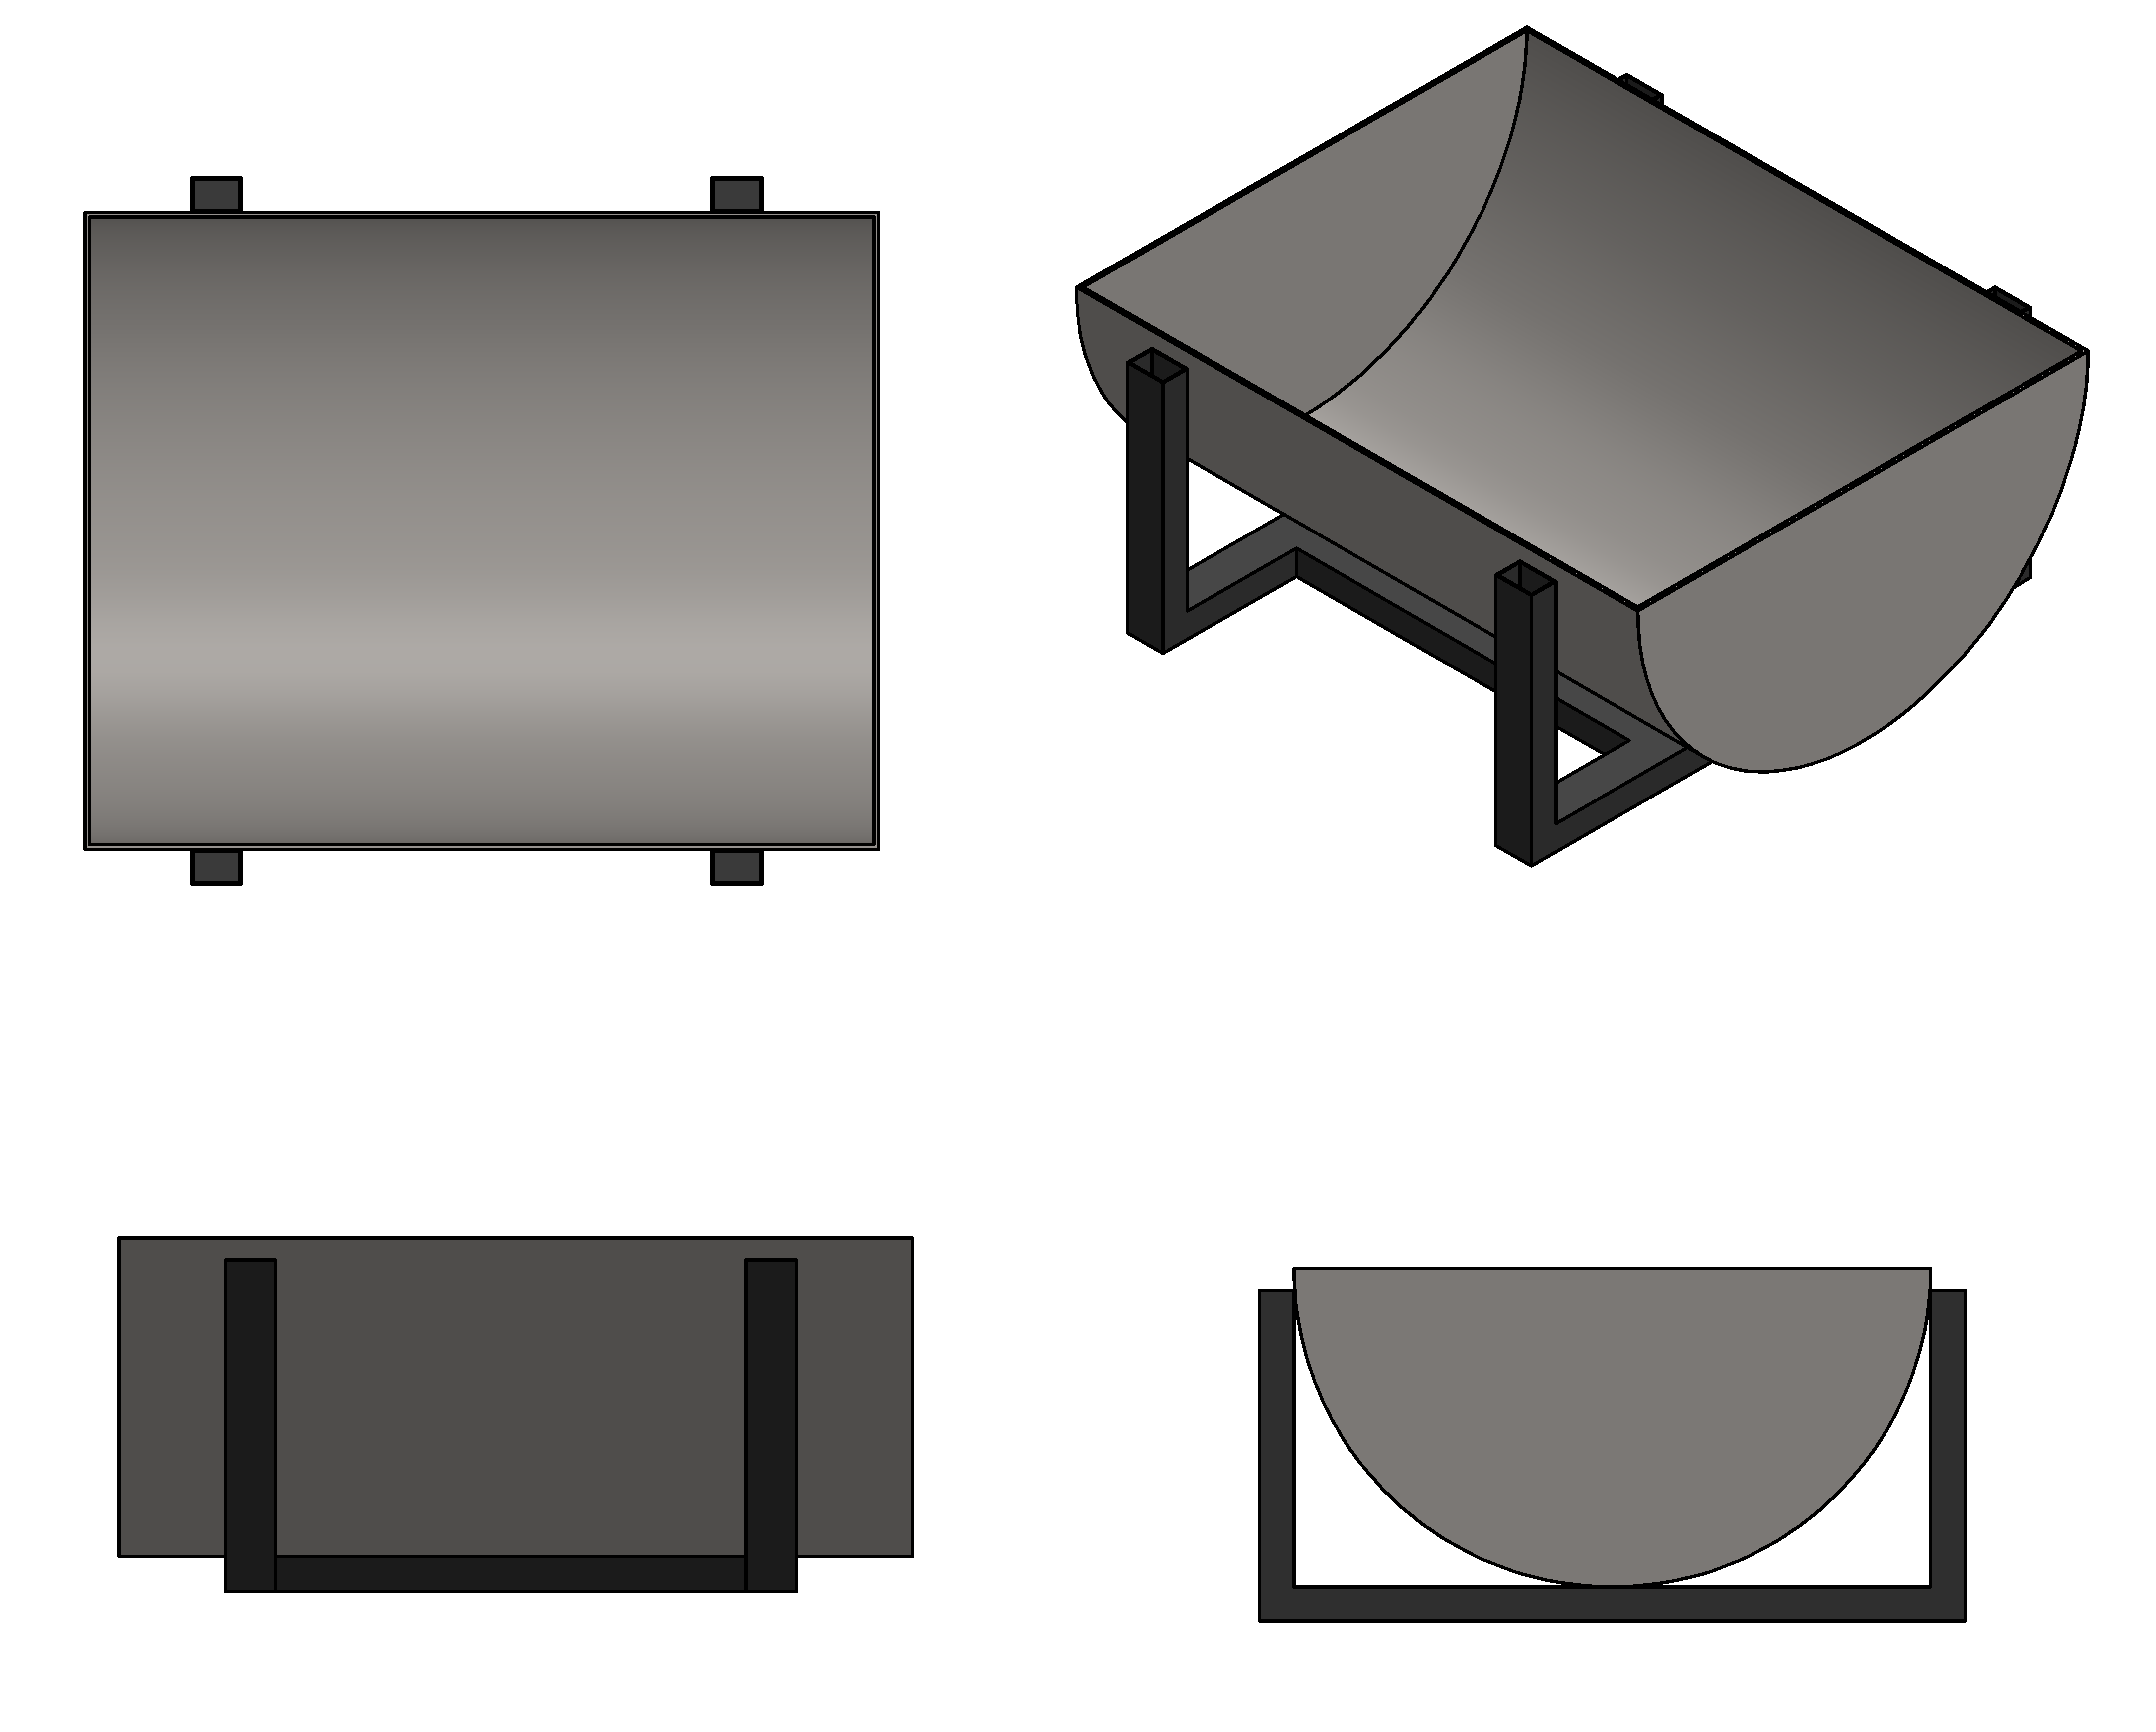
\includegraphics{Figures/CollectionTank.PNG}
    \caption{Collection tank}
    \label{fig:collection_tank}
\end{figure}
\par
\item \textbf{Position}
\par
The positioning of the tank was also a critical aspect of the design. Ideally, the collection tank was to be either positioned directly just below the flow diversion unit or at the periphery of the main reservoir. Positioning the collection tank directly below the flow diversion unit mitigates the need for additional components such as diverting pipes. This simply implies that the collection tank would just be provided with a holding mechanism for support upon which it is fitted with a solenoid outlet valve directly into the reservoir. On the contrary, positioning the collection tank on the periphery introduces the need for additional components. This includes a pump system to pump the discharge back into the reservoir, which adds to the overall cost of the project. Positioning the collection tank below the diversion unit was the feasible option.
\end{itemize}

\subsubsection{Outlet valve sub-unit}
This valve is attached to the collection tank and is used to empty the tank into the main reservoir. The main consideration was the response time(time taken to close and open the valve) in the selection of a valve suitable for this application. The following options were feasible:
\begin{enumerate}
    \item \textbf{An electrically Controlled Butterfly valve}
    \par
    \begin{figure}[H]
        \centering
        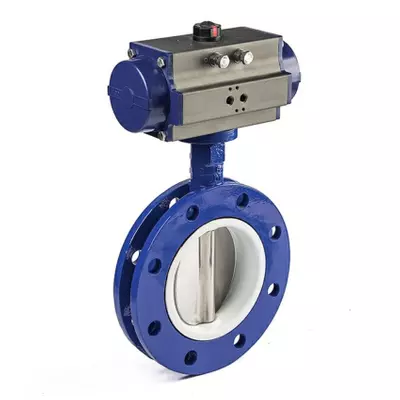
\includegraphics[width=0.25\textwidth, height=.25\textheight]{Figures/butterflyValve.png}
        \caption[Butterfly valve]{Butterfly valve \cite{butterfly}}
        \label{fig:butterfly_valve}
    \end{figure}
    The operating voltage of the valve shown in figure \ref{fig:butterfly_valve} is in the range 12V DC - 230V AC. Therefore, its response time can be reduced by increasing the voltage supply to the solenoid.
    \item \textbf{A solenoid gate valve(with a plunger)}
    \par
    \begin{figure}[H]
        \centering
        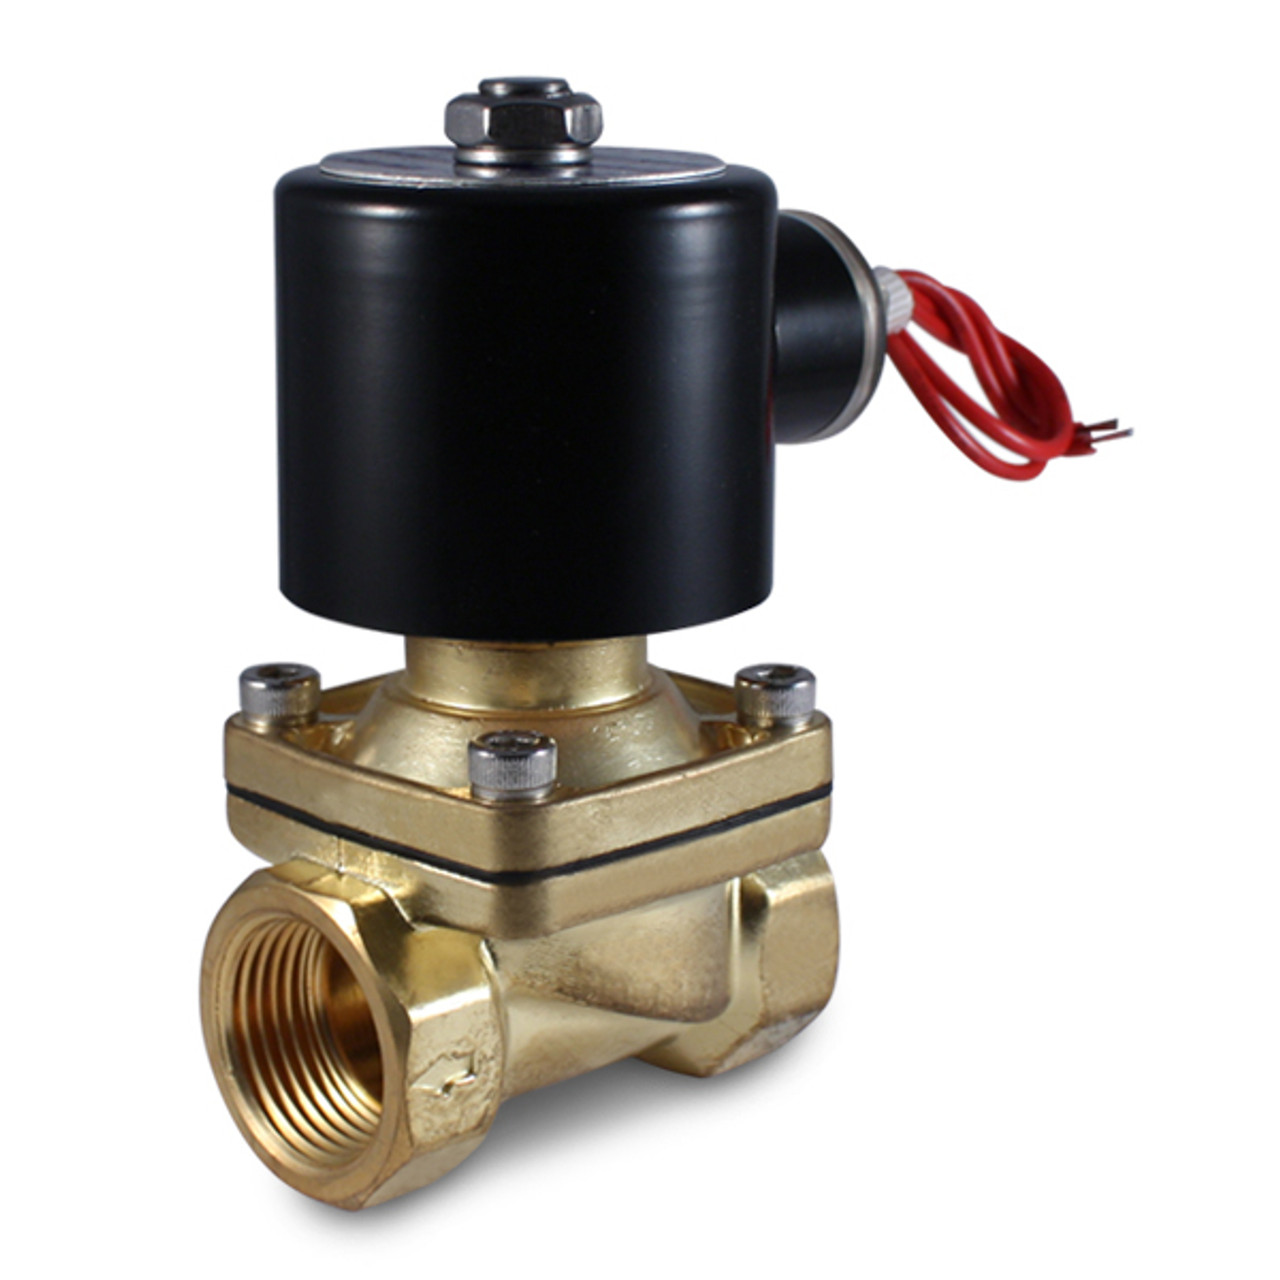
\includegraphics[width=.25\textwidth, height=.25\textheight]{Figures/solenoidValve.jpg}
        \caption[Solenoid valve]{Solenoid valve \cite{solenoid}}
        \label{fig:solenoid_valve}
    \end{figure}
    The $\frac{3}{4} inch$ solenoid valve shown in figure \ref{fig:solenoid_valve} uses a plunger with a cork for control the flow. How fast the plunger closes the aperture depends on the voltage supplied to the solenoid. The operating voltage of this type of valve is 12V DC.
\end{enumerate}

The solenoid gate valve(with a plunger) was selected for this application mainly because the butterfly valve is expensive relative to the budget set for the project.

\subsubsection{Weight measurement sub-unit}
The weight of the collected discharge is measured in every step in an experiment done on this machine. The weight can be cumulative or measured per step. In the event of an error, the error is not propagated in the cumulative approach, but it will definitely be propagated to every measurement in the weight-per-step approach. Therefore, the weight-per-step approach was selected for this application.
\par
During the selection of a method to use for weight measurement of the discharge, the following considerations were made:
\begin{enumerate}
    \item The maximum weight that can be precisely measured by the unit. The maximum weight of the structure to be measured is determined as follows:\\
    \begin{align*}
    \text{Assume the maximum volume of the water collected} = 0.01m^{3}.\\
    Mass(M) = Density(\rho) \times Volume(V)\\
    \text{Water density} (\rho_{\textit{water}}) = 1000kg/m^{3}\\
    \therefore  \text{Mass of water} (M_{\textit{water}}) = \rho_{\textit{water}} \times \text{Volume of water} (V_{\textit{water}}) \\
    = 0.01m^{3} \times 1000kg/m^{3} \\
    = 10 Kg
    \end{align*}
    The measuring device should therefore handle weights of more than 10Kg.
    \item The resolution of the device.
    \item The credibility of the weight measurement device.
\end{enumerate}
On the basis of the above considerations, the following options were considered:
\begin{enumerate}
    \item Weight measurement by ultrasonic waves
    \par
    Ultrasonic waves can be used to determine the depth of discharge in the tank. An ultrasonic wave generator generates an ultrasonic wave and is propagated to the surface of the water. It is then reflected due to refraction to a receiver. The time taken to send and receive the echo is multiplied by the speed of sound to obtain the depth of the empty side of the container. \par 
    This approach is rudimentary and very much flawed as there are many considerations in order to obtain almost accurate results. Some of the considerations include:
    \begin{enumerate}
        \item The angle of reflexion $\delta$ is shown in figure \ref{fig:ultrasonic sensor measurement model}.
        \begin{figure}[H]
            \centering
            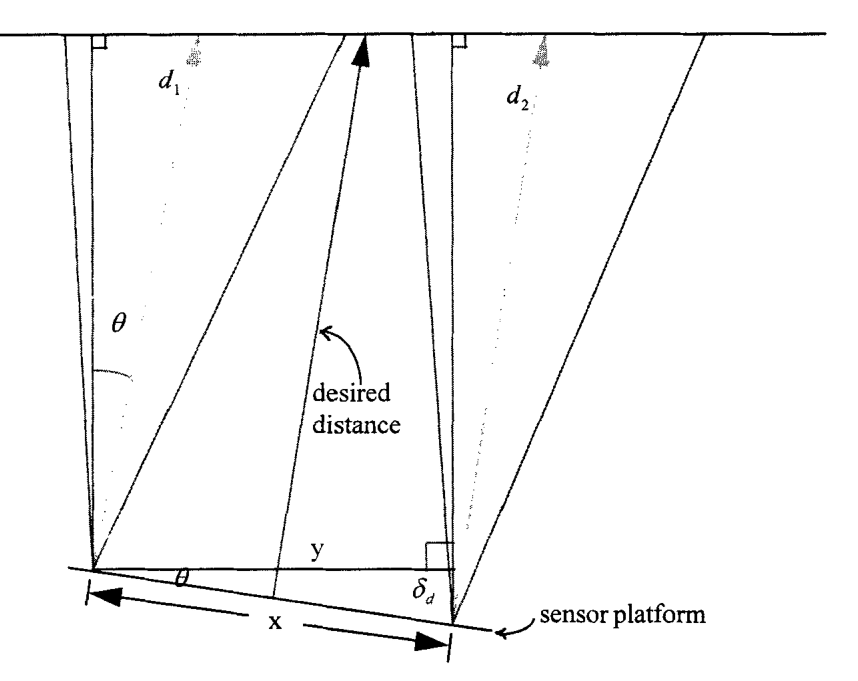
\includegraphics{Figures/angleOfReflection-1.png}
            \caption[Ultrasonic sensor measurement model]{Ultrasonic sensor measurement model \cite{chang1996ultrasonic}}
            \label{fig:ultrasonic sensor measurement model}
        \end{figure}
        \item The Gaussian noise to environmental changes. There is an almost 3.5\% increase in noise for a temperature difference of only $20^{0}$ \cite{chang1996ultrasonic}.
    \end{enumerate}
    To use this approach requires calibration of many parameters, some of which are to be done in real time. A mathematical model would be preferable for this calibrations.
    \item Load cells
    \par
    These are transducers capable of converting pressure to an electrical signal specifically a strain in its material structure is converted to electrical resistance.
    \par
    The loading cell disc shown in Figure \ref{fig:load_cell_disc} with a load force range of 0-50Kg was selected for application due to its weight range.
    \begin{figure}[H]
        \centering
        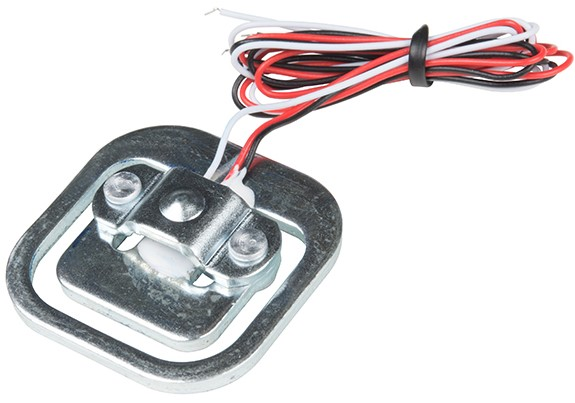
\includegraphics[width=.25\textwidth, height=.25\textheight]{Figures/50KgLoadCell.jpg}
        \caption[Strain-type load cells]{Strain-type load cells \cite{loadcell}}
        \label{fig:load_cell_disc}
    \end{figure}
\end{enumerate}
The use of a load cell was selected for this application based on the merits listed in the descriptions above. However, a single-load cell disc will be inefficient in measuring the weight of this load. Therefore, four load cells were selected to strategically position at the edges of the support frame of the discharge collection tank, as shown in Figure \ref{fig:collection_tank_with_load_cells}.
\begin{figure}[H]
    \centering
    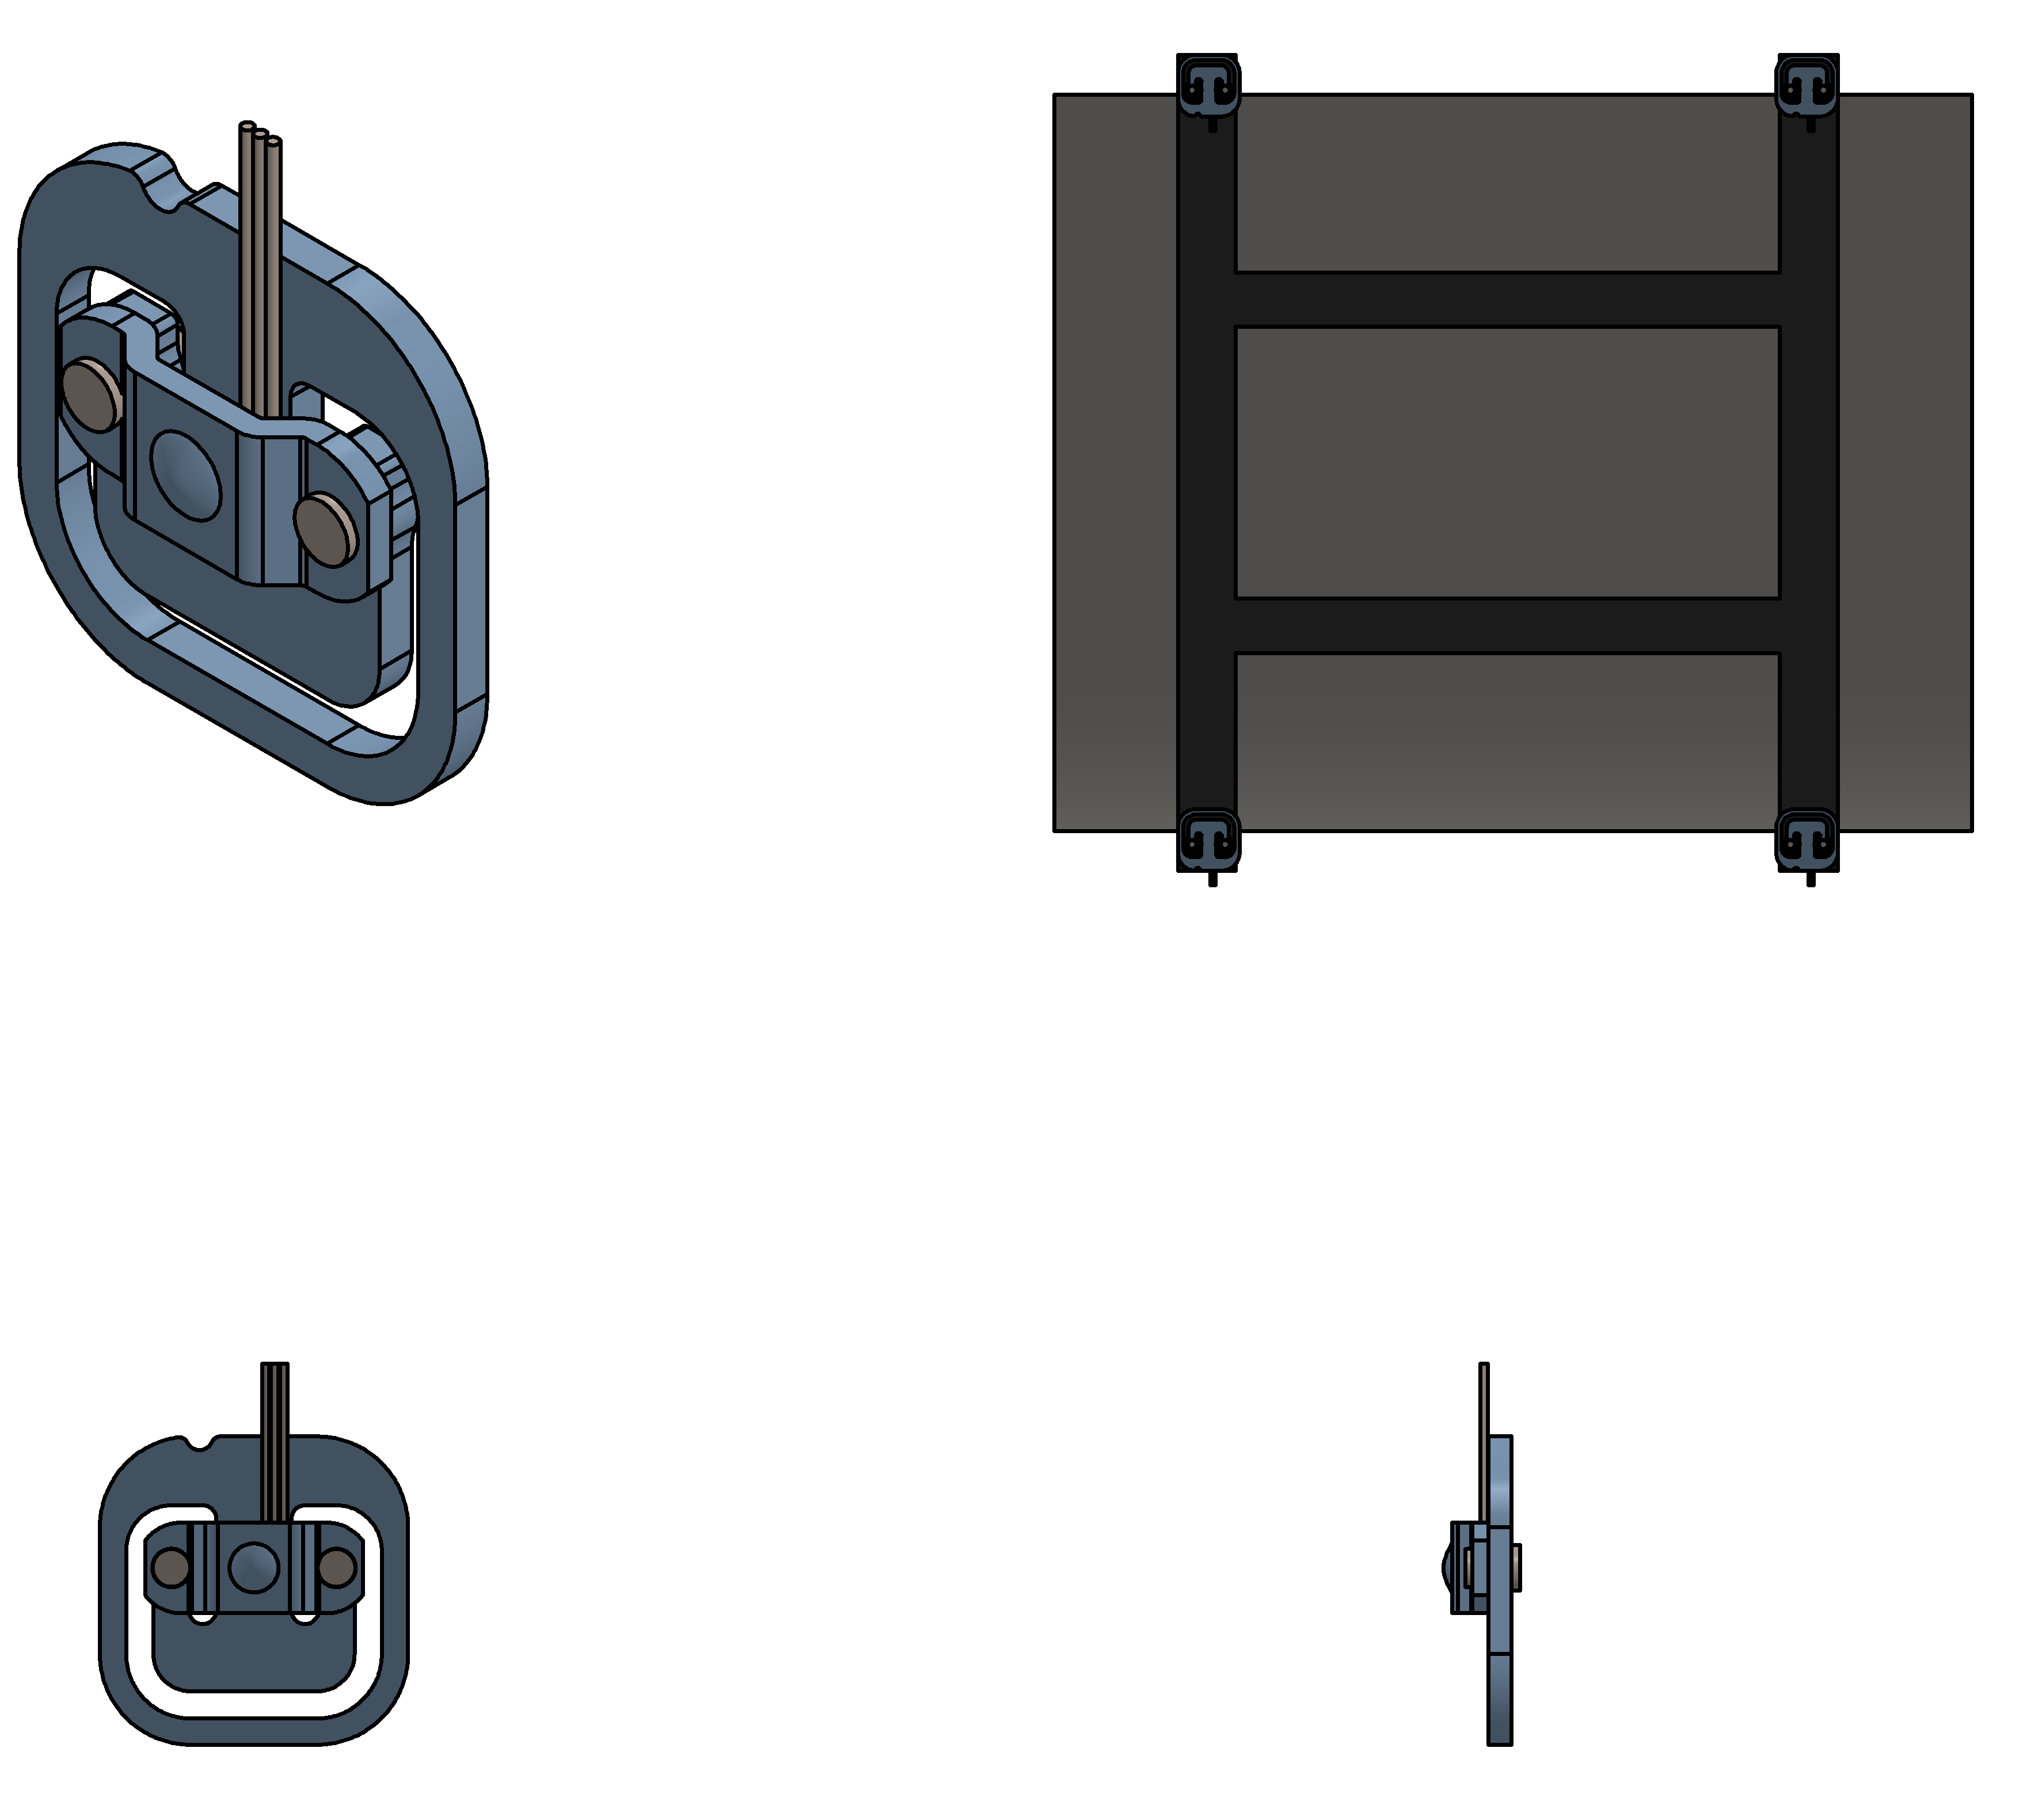
\includegraphics[height=.45\textheight]{Figures/CollectionTankWithTheLoadCells.PNG}
    \caption{Collection tank with load cells}
    \label{fig:collection_tank_with_load_cells}
\end{figure}

\subsubsection{Temperature measurement sub-unit}
In the same way as weight measurement of the discharge, the temperature of the discharge is measure in every step. This is relevant in ensuring consistency of the data collected in an experiment done in this machine. 
\par
Since this measurement is taken within roughly 10 seconds before the outlet valve is opened, a measuring device whose sensitivity is enough to establish reliable results within that time is required for this application.
\par
A couple of temperature measurement sensors were considered for this application but an immersible DS18B20 temperature probe shown in figure \ref{fig:ds18b20_temperature} was selected. Its technical specifications are shown in table \ref{tab:ds18b20 temperature probe}.
\begin{figure}[H]
    \centering
    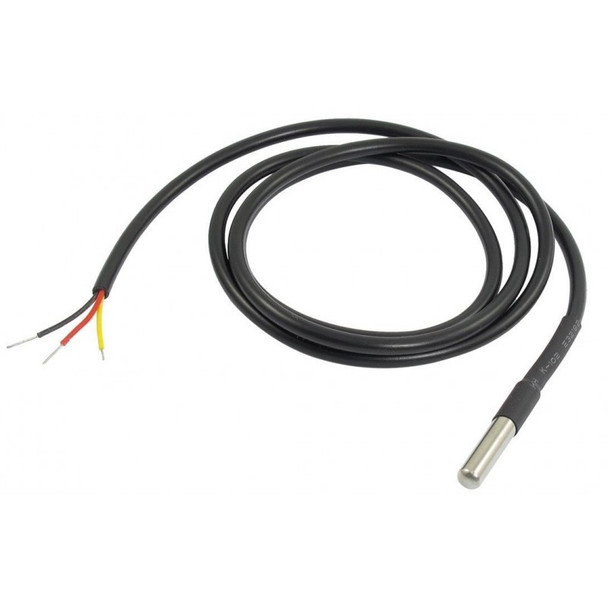
\includegraphics[width=.25\textwidth, height=.25\textheight]{Figures/ds18b20_temperature_probe.jpg}
    \caption[DS18B20 temperature probe]{DS18B20 temperature probe \cite{ds18b20}}
    \label{fig:ds18b20_temperature}
\end{figure}
\begin{table}[H]
\centering
\begin{tabular}{|l|l|}
\hline
\textbf{Property} & \textbf{Value} \\ \hline
Operating voltage & 3.3V  to 5V DC \\ \hline
Operating temperature range & -55°C to +125°C (-67°F to +257°F) \\ \hline
Accuracy over the range of -10°C to +85°C: & ±0.5°C. \\ \hline
Water proof & True \\ \hline
\end{tabular}
\caption[DS18B20 temperature range specifications]{DS18B20 temperature range specifications \cite{ds18b20}}
\label{tab:ds18b20 temperature probe}
\end{table}

\subsubsection{Electrical}
\begin{enumerate}
    \item \textbf{Solenoid valve connection}
    \par
    \begin{itemize}
        \item \textbf{Power requirements}
        \par
        The selected solenoid valve operates on 12V DC voltage. This requires an external supply and circuit to activate the supply when needed.
        \item \textbf{Circuit}
        \par
        An IRF520 N-Ch power module described previously can be used to power this device with a 12V supply.
    \end{itemize}
    \item \textbf{Strain type load cell connection}
    \par
    \begin{itemize}
        \item \textbf{Power requirements}
        \par
        The four load cells used in this application are connected through a load combinator module whose operating voltage is between 2.7V to 5V.
        \item \textbf{Circuit}
        \par
        The load cells are connected in a Wheat-stone bridge through a load combinator module as shown in figure \ref{fig:load_cell_circuit}.
        \begin{figure}[H]
            \centering
            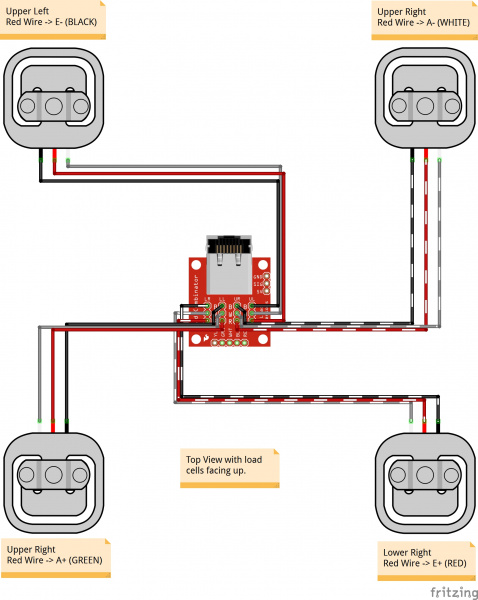
\includegraphics[width=.65\textwidth, height=.65\textheight]{Figures/load_cell_combined.jpg}
            \caption[Load cells circuit]{Load cells circuit \cite{loadcell}}
            \label{fig:load_cell_circuit}
        \end{figure}
    \end{itemize}
    \item \textbf{DS18B20 temperature probe connection}
    \par
    \begin{itemize}
        \item \textbf{Power requirements}
        \par
        This sensor's operating voltage is between 3.0V and 5V. Therefore Vcc line can be connected directly to the 5V pin of the micro-controller.
    \end{itemize}
\end{enumerate}
\subsubsection{Software and control}
\begin{itemize}
    \item \textbf{Calibration}
    \par
    The load cells and the temperature sensor are calibrated once the whole system is assembled.
    \item \textbf{Auto calibration}
    \par 
    This can be achieved by having weight and temperature measurements triggered by an event and only measuring differential values.
    \item \textbf{Mean}
    \par
    In this application, the weight and temperature of the discharge is measured over a period of time before the value of a measurement is determined. The noise in the variation within that time can be minimized by using a calibrated Kalman's filter.
\end{itemize}

\subsection{Interface and Control Unit}
This unit consists of two subunits:
\begin{enumerate}
    \item Interface sub-unit
    \item Controller sub-unit
\end{enumerate}

\subsubsection{Interface sub-unit}
This sub-unit provides a means of interaction between the system and the user. Ideally, the subunit enables the user to input instructions and control the processes in this system. The status and results of processes in this system are also displayed in the interface. The choice of an interface depended on the following factors:
\begin{enumerate}
    \item Size \\
    This is the size of the operable part of the interface. In case of touch interface, a minimum of a 320x240 LCD is required to enable at least the minimum operability of GUI items, and a 20x4 LCD for any other choice.
    \item Ergonomics \\
    This refers to the impact of the interface on the user, the ease and efficiency in operating it. For an interface for this application, the user should be able to spend the least possible time feeding input and reading the results with relative ease. 
    \item Aesthetics \\
    This is the perception of the user while operating the interface, their feeling about the interface. For this application, the interface will be used most frequently by students with limited exposure. A good look might be motivating. However, this should not compromise the design. It should be able to be introduced and improved with minimum modifications to the hardware in the system. 
\end{enumerate}
Based on the above considerations, the following options were considered:
\begin{enumerate}
    \item LCD With keypad 
    \par
    This type of interface is shown in figure \ref{fig:lcd_with keypad}. One can navigate, read and provide input where it is required on the LCD display using the keypad.
    \begin{figure}[H]
        \centering
        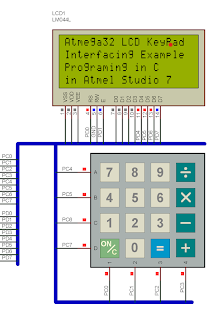
\includegraphics[width=.25\textwidth,height=.25\textheight]{Figures/controlInterface.png}
        \caption[LCD with keypad]{LCD with keypad \cite{lcd_with_keypad}}
        \label{fig:lcd_with keypad}
    \end{figure}
    \item LCD with touch 
    \par
    This type of interface is shown in figure \ref{fig:lcd_with_touch}. One can navigate such interface easily by touching or use a virtual keyboard to provide input. 
    \begin{figure}[H]
        \centering
        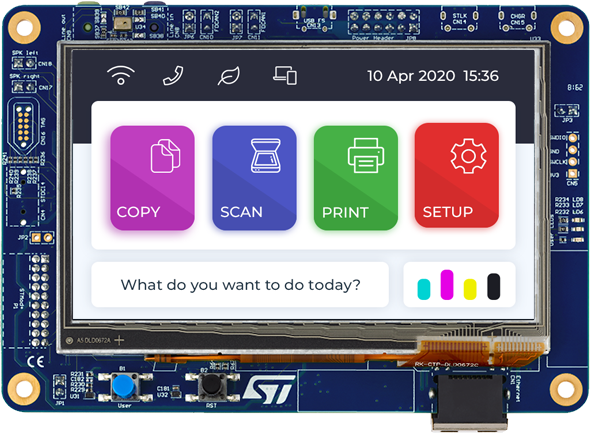
\includegraphics[width=0.55\textwidth,height=.35\textheight]{Figures/lcdWithTouch.png}
        \caption[LCD with touch]{LCD with touch \cite{lcd_with_touch}}
        \label{fig:lcd_with_touch}
    \end{figure}
     This type of LCD communicates with the microcontroller through an 8-bit parallel interface and four ports(32 pins). This can sometimes be replaced by an HDMI interface depending on the size of the screen.
    \item LCD with Knob
    \par
    This interface shown in Figure \ref{fig:lcd_with_knobs} is controlled by a knob. Navigation from page to page,field to field is achieved by turning the knob. To provide an input in a field, the knob can be pressed and turned. This is common in low-budget 3D printers.
    \begin{figure}[H]
        \centering
        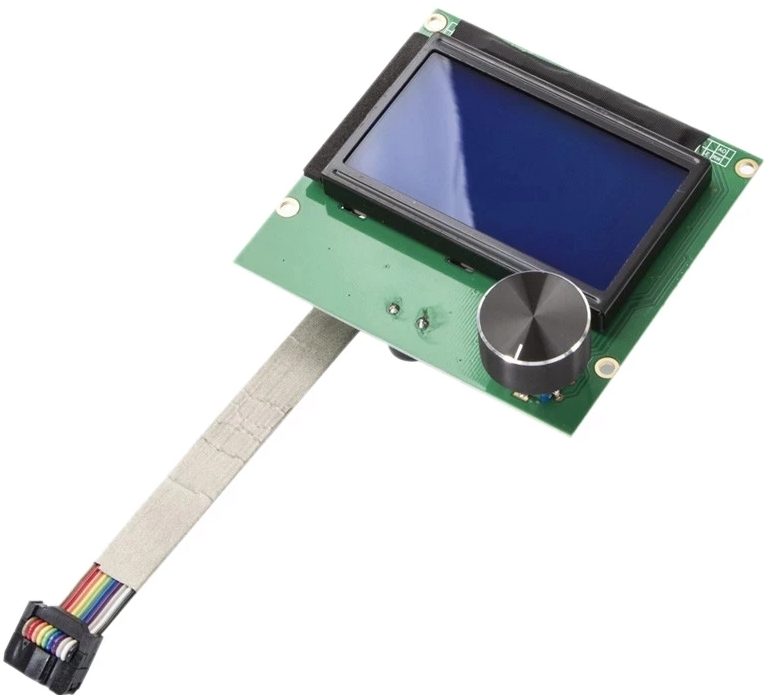
\includegraphics[width=0.25\textwidth,height=.25\textheight]{Figures/lcdwithknob.png}
        \caption[Lcd with knob]{LCD with knob \cite{noauthor_prusa_nodate}}
        \label{fig:lcd_with_knobs}
    \end{figure}
\end{enumerate}

 An efficient choice for this application was to use a touch LCD interface. This choice satisfies all the requirements required of an interface for this application. In addition, one can also improve the aesthetics of the design by simply tweaking the GUI software without major hardware changes.
 \par
 Touch LCDs can be very expensive relative to our budget and challenging to programme. Two variations of touch LCDs are available for our application: those with a 32-pin interface and those with an HDMI interface. Those with HDMI interface are available in sizes larger than 7 inches and are priced at not less than \$90. Those with 32-pin interface are available to sizes as small as 1.77 inches and are relatively cheaper.    
\begin{itemize}
    \item \textbf{LCD GUI design}
    \par
    A preliminary GUI is shown in Figure \ref{fig:GUI_interface}.
    \begin{figure}[H]
        \centering
        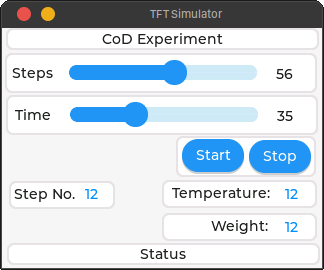
\includegraphics{Figures/interfacedesign.png}
        \caption{GUI interface}
        \label{fig:GUI_interface}
    \end{figure}
    The design is in a 320x240 frame, the size of the selected LCD. The steps sizes and time interval's inputs can be provided by sliding on the sliding bar. The value of a position on the slider is displayed inside the slider handle.
    \par
    The step number, weight and temperature of that specific step are also displayed once a step is complete.
    \par
    In case of any errors in the system, an error message is displayed at the bottom of the frame.
\end{itemize}

\subsubsection{Controller sub-unit}
This sub-unit executes the application logic, sends instructions to the actuators, and reads inputs from sensors in the system. It is responsible for synchronising the GUI with the processes in the hardware. This unit monitors and controls the parameters of the input devices and generates output signals to implement desired tasks.
\par
The choice of a micro-controller for this application was guided by the selected interface, a touch LCD. Figure \ref{fig:mcu selection} shows the selection procedure for a micro-controller for this application.

\begin{figure}[H]
    \centering
    \includegraphics[width=\textwidth,height=\textheight, keepaspectratio]{Figures/BoardSelection.png}
    \caption{Board Selection}
    \label{fig:mcu selection}
\end{figure}

\begin{itemize}
    \item \textbf{Graphics library} 
    \par
    To develop graphics for a touch LCD, the choice of graphics libraries was between the Light and Versatile Embedded Graphics Library (LVGL) and the Qt/QML graphics libraries. These two are versatile and have great community support. Each library supports specific display drivers out-of-the-box. For this application, an LCD with an ILI9341 driver had been selected, therefore support for this specific driver was necessary. Drivers for a specific driver could also be developed from scratch in a long and tedious process. To avoid this, out-of-the-box support was required. LVGL tends to offer that support; therefore, it was selected as the graphics library for this application.
    \item \textbf{Board support} 
    \par
    LVGL library also provides support for specific board families out of the box, such as the NXP and STM32F4 families. LVGL support for these boards automatically means that this board has the number of ports required for LCD touch functionality.
    \item \textbf{Platform support}
    \par
    LVGL is just a graphics library. The board is required to support other peripherals such as the electromagnet, servo motor, weight and temperature measurement devices, and the solenoid valve. This can be done in an RTOS platform such Zephyr(C/C++) or Mbed(C++). However, these platforms support specific boards out-of-the-box, but custom boards could also be added. To make the project a little easier, an out-of-the-box was required. The two platforms tend to support the two boards. 
    \item \textbf{Price}
    \par
    This is the most crucial part of this selection. Both boards can be considered expensive relative to the project's budget, but the STM32F4 family boards can be relatively cheaper. Therefore, an STM32F407VET6 board was selected.
\end{itemize}

\subsubsection{Electrical}
\begin{itemize}
    \item \textbf{Touch LCD connection}
    \par
    STM32F407VET6 board provides a dedicated interface for touch LCD with FSMC interface as shown in figure \ref{fig:fsmc_interface}.
    \begin{figure}[H]
        \centering
        \includegraphics[width=.45\textwidth, height=.325\textheight]{Figures/STM32F407VET6.png}
        \caption[Load cells circuit]{FSMC interface in STM32F407VET6 \cite{mcu_lcd}}
        \includegraphics[width=.45\textwidth, height=.325\textheight]{Figures/stm32f407vet6_with_lcd.png}
        \caption[STM32 connected with LCD]{STM32 connected with LCD \cite{mcu_lcd}}
        \label{fig:fsmc_interface}
    \end{figure}
\end{itemize}

\subsubsection{Software and control}
The logic of the whole application is shown in figure \ref{fig:application_logic}.

\begin{figure}[H]
    \centering
    \includegraphics[width=\textwidth, height=0.8\textheight, keepaspectratio]{Figures/ApplicationLogic.png}
    \caption{Application logic}
    \label{fig:application_logic}
\end{figure}

The application requires the user to set the number of steps of the experiment or the time interval between the steps. This is done by sliding the slide handle of one of the inputs in the touch GUI. When the user presses the handle on the input of the steps, the system automatically adjusts the time interval between the steps and vice versa.
\par
Once the steps are set, the user clicks on the start button. The system then turns the valve by one step after starting the timer. This is done simultaneously with commencement of the discharge collection and the measurement of the discharge temperature.
\par
The system will continuously check if the time interval has elapsed and if it has, it will simultaneously stop the discharge collection and the temperature measurement.  It will then compute the differential change in temperature and measure the weight of the discharge. The results of this measurement are displayed in the GUI. \par
This is repeated for the set steps but the user has the option to cancel the experiment.

